%%%%%%%%%%%%%%%%%%%%%%%%%%%%%%%%%%%%%%%%%%
% The Legrand Orange Book
% LaTeX Template
% Version 2.4 (26/09/2018)
%
% This template was downloaded from:
% http://www.LaTeXTemplates.com
%
% Original author:
% Mathias Legrand (legrand.mathias@gmail.com) with modifications by:
% Vel (vel@latextemplates.com)
%
% License:
% CC BY-NC-SA 3.0 (http://creativecommons.org/licenses/by-nc-sa/3.0/)
%
% Compiling this template:
% This template uses biber for its bibliography and makeindex for its index.
% When you first open the template, compile it from the command line with the 
% commands below to make sure your LaTeX distribution is configured correctly:
%
% 1) pdflatex main
% 2) makeindex main.idx -s StyleInd.ist
% 3) biber main
% 4) pdflatex main x 2
%
% After this, when you wish to update the bibliography/index use the appropriate
% command above and make sure to compile with pdflatex several times 
% afterwards to propagate your changes to the document.
%
% This template also uses a number of packages which may need to be
% updated to the newest versions for the template to compile. It is strongly
% recommended you update your LaTeX distribution if you have any
% compilation errors.
%
% Important note:
% Chapter heading images should have a 2:1 width:height ratio,
% e.g. 920px width and 460px height.
%
%%%%%%%%%%%%%%%%%%%%%%%%%%%%%%%%%%%%%%%%%

%----------------------------------------------------------------------------------------
%	PACKAGES AND OTHER DOCUMENT CONFIGURATIONS
%----------------------------------------------------------------------------------------

\documentclass[11pt,fleqn]{book} % Default font size and left-justified equations





\usepackage[dvipsnames]{xcolor}






           %%%%%%%%%%%%%%%%%%%%%%%%%%%%%%%%%%%%%%%%%
% The Legrand Orange Book
% Structural Definitions File
% Version 2.1 (26/09/2018)
%
% Original author:
% Mathias Legrand (legrand.mathias@gmail.com) with modifications by:
% Vel (vel@latextemplates.com)
% 
% This file was downloaded from:
% http://www.LaTeXTemplates.com
%
% License:
% CC BY-NC-SA 3.0 (http://creativecommons.org/licenses/by-nc-sa/3.0/)
%
%%%%%%%%%%%%%%%%%%%%%%%%%%%%%%%%%%%%%%%%%

%----------------------------------------------------------------------------------------
%	VARIOUS REQUIRED PACKAGES AND CONFIGURATIONS
%----------------------------------------------------------------------------------------

\usepackage{graphicx} % Required for including pictures
\graphicspath{{Pictures/}} % Specifies the directory where pictures are stored

\usepackage{lipsum} % Inserts dummy text

\usepackage{tikz} % Required for drawing custom shapes

\usepackage[english]{babel} % English language/hyphenation

\usepackage[shortlabels]{enumitem}


% \usepackage{enumitem} % Customize lists
\setlist{nolistsep} % Reduce spacing between bullet points and numbered lists

\usepackage{booktabs} % Required for nicer horizontal rules in tables

\usepackage{xcolor} % Required for specifying colors by name
\definecolor{ocre}{RGB}{243,102,25} % Define the orange color used for highlighting throughout the book
\linespread{1.25}
%----------------------------------------------------------------------------------------
%	MARGINS
%----------------------------------------------------------------------------------------

\usepackage{geometry} % Required for adjusting page dimensions and margins

\geometry{
	paper=a4paper, % Paper size, change to letterpaper for US letter size
	%paper=letterpaper,
	top=3cm, % Top margin
	bottom=3cm, % Bottom margin
	left=3cm, % Left margin
	right=3cm, % Right margin
	headheight=14pt, % Header height
	footskip=1.4cm, % Space from the bottom margin to the baseline of the footer
	headsep=10pt, % Space from the top margin to the baseline of the header
	%showframe, % Uncomment to show how the type block is set on the page
}




\usepackage[normalem]{ulem}
\usepackage{amsmath}
\usepackage[english]{babel}
\usepackage{graphicx}
\usepackage{tabulary}
\usepackage{tabularx}
\usepackage{cancel}
\usepackage{pagecolor}
\usepackage{afterpage}
\usepackage{soul}
\usepackage{fixltx2e}
\usepackage[utf8]{inputenc}
\usepackage{siunitx} %degrees for Laboratory
\usepackage{pdflscape} %sidescape figure in Laboratory
\usepackage{float}
\usepackage{placeins}
\usepackage{afterpage}
\usepackage{xcolor}
\usepackage{framed}
\usepackage{soul}
%\textsubscript{this}
\usepackage{lastpage}
\usepackage[utf8]{inputenc}
\usepackage{ifthen}
\usepackage{amsmath}
\usepackage{fancyhdr}
\usepackage[document]{ragged2e}
% \usepackage[margin=1in,top=1.2in,headheight=57pt,headsep=0.1in]{geometry}
\usepackage{fancyhdr}
\usepackage{caption}
\usepackage{subcaption}
%Chapter 2
\usepackage{rotating}%for sidewaysfigure
\usepackage[final]{pdfpages}
\usepackage{gensymb}
\usepackage[most]{tcolorbox}
%\usepackage[dvipsnames]{xcolor}
\usepackage{colortbl}
\usepackage{chemfig}
\usepackage{lscape}
\usepackage{wrapfig}
\usepackage{float}
% FOR CENTERING TEXT IN TABLE
\usepackage{array}
\usepackage{multirow}
\newcolumntype{C}[1]{>{\centering\arraybackslash}m{#1}}
\usepackage{amsfonts}
\usepackage{amssymb}
\usepackage{mhchem}
\usepackage{stmaryrd}
\usepackage{graphicx}
\usepackage[export]{adjustbox}
\graphicspath{ {./images/} }
\usepackage{makecell}
\usepackage{hyperref}
\usepackage[justification=centering]{caption}
\usepackage{booktabs}% http://ctan.org/pkg/booktabs
\usepackage{wrapfig}
\usepackage{setspace}
\usepackage{pifont}
\usepackage{animate}
\usepackage{imakeidx}
\makeindex\makeindex[columns=3, title=Alphabetical Index, 
           options= -s example_style.ist]
\newcommand{\tabitem}{~~\llap{\textbullet}~~}
\graphicspath{ {./images/} }
%\usetikzlibrary{positioning}
%\usetikzlibrary{decorations.pathreplacing}
%\usetikzlibrary{automata}
%\usetikzlibrary {shapes.multipart}
%\usetikzlibrary{calc}
%\usetikzlibrary{arrows}
%\usetikzlibrary{snakes}
%\usetikzlibrary{calc}
\usetikzlibrary{shapes.multipart, shapes.geometric, arrows}
\usetikzlibrary{calc, decorations.markings}
\usetikzlibrary{arrows.meta}
\usetikzlibrary{shapes,snakes}
\usetikzlibrary{quotes,angles, positioning}
\usetikzlibrary{arrows.meta,
                chains,
                positioning,
                shapes.geometric
                }

\makeatletter
\pgfkeys{/pgf/.cd,
  parallelepiped offset x/.initial=4mm,
  parallelepiped offset y/.initial=4mm
}
\pgfdeclareshape{parallelepiped}
{
  \inheritsavedanchors[from=rectangle] % this is nearly a rectangle
  \inheritanchorborder[from=rectangle]
  \inheritanchor[from=rectangle]{north}
  \inheritanchor[from=rectangle]{north west}
  \inheritanchor[from=rectangle]{north east}
  \inheritanchor[from=rectangle]{center}
  \inheritanchor[from=rectangle]{west}
  \inheritanchor[from=rectangle]{east}
  \inheritanchor[from=rectangle]{mid}
  \inheritanchor[from=rectangle]{mid west}
  \inheritanchor[from=rectangle]{mid east}
  \inheritanchor[from=rectangle]{base}
  \inheritanchor[from=rectangle]{base west}
  \inheritanchor[from=rectangle]{base east}
  \inheritanchor[from=rectangle]{south}
  \inheritanchor[from=rectangle]{south west}
  \inheritanchor[from=rectangle]{south east}
  \backgroundpath{
    % store lower right in xa/ya and upper right in xb/yb
    \southwest \pgf@xa=\pgf@x \pgf@ya=\pgf@y
    \northeast \pgf@xb=\pgf@x \pgf@yb=\pgf@y
    \pgfmathsetlength\pgfutil@tempdima{\pgfkeysvalueof{/pgf/parallelepiped offset x}}
    \pgfmathsetlength\pgfutil@tempdimb{\pgfkeysvalueof{/pgf/parallelepiped offset y}}
    \def\ppd@offset{\pgfpoint{\pgfutil@tempdima}{\pgfutil@tempdimb}}
    \pgfpathmoveto{\pgfqpoint{\pgf@xa}{\pgf@ya}}
    \pgfpathlineto{\pgfqpoint{\pgf@xb}{\pgf@ya}}
    \pgfpathlineto{\pgfqpoint{\pgf@xb}{\pgf@yb}}
    \pgfpathlineto{\pgfqpoint{\pgf@xa}{\pgf@yb}}
    \pgfpathclose
    \pgfpathmoveto{\pgfqpoint{\pgf@xb}{\pgf@ya}}
    \pgfpathlineto{\pgfpointadd{\pgfpoint{\pgf@xb}{\pgf@ya}}{\ppd@offset}}
    \pgfpathlineto{\pgfpointadd{\pgfpoint{\pgf@xb}{\pgf@yb}}{\ppd@offset}}
    \pgfpathlineto{\pgfpointadd{\pgfpoint{\pgf@xa}{\pgf@yb}}{\ppd@offset}}
    \pgfpathlineto{\pgfqpoint{\pgf@xa}{\pgf@yb}}
    \pgfpathmoveto{\pgfqpoint{\pgf@xb}{\pgf@yb}}
    \pgfpathlineto{\pgfpointadd{\pgfpoint{\pgf@xb}{\pgf@yb}}{\ppd@offset}}
  }
}
\makeatother









%Defining colour with different models.
\definecolor{mypink1}{rgb}{0.858, 0.188, 0.478}
\definecolor{mypink2}{RGB}{219, 48, 122}
\definecolor{mypink3}{cmyk}{0, 0.7808, 0.4429, 0.1412}
\definecolor{mygray}{gray}{0.6}
\colorlet{LightRubineRed}{RubineRed!70!}
\colorlet{Mycolor1}{green!10!orange!90!}
\definecolor{Mycolor2}{HTML}{00F9DE}
%\fboxsep=4mm%padding thickness
%\fboxrule=4pt%border thickness

%New command used in the table with all available colour names
\newcommand{\thiscolor}[1]{\texttt{#1} \hfill \fcolorbox{black}{#1}{\hspace{2mm}}}
%----------------------------------------------------------------------------------------
%	FONTS
%----------------------------------------------------------------------------------------

\usepackage{avant} % Use the Avantgarde font for headings
%\usepackage{times} % Use the Times font for headings
\usepackage{mathptmx} % Use the Adobe Times Roman as the default text font together with math symbols from the Sym­bol, Chancery and Com­puter Modern fonts

\usepackage{microtype} % Slightly tweak font spacing for aesthetics
\usepackage[utf8]{inputenc} % Required for including letters with accents
\usepackage[T1]{fontenc} % Use 8-bit encoding that has 256 glyphs

%----------------------------------------------------------------------------------------
%	BIBLIOGRAPHY AND INDEX
%----------------------------------------------------------------------------------------

\usepackage[style=numeric,citestyle=numeric,sorting=nyt,sortcites=true,autopunct=true,babel=hyphen,hyperref=true,abbreviate=false,backref=true,backend=biber]{biblatex}
\addbibresource{bibliography.bib} % BibTeX bibliography file
\defbibheading{bibempty}{}

\usepackage{calc} % For simpler calculation - used for spacing the index letter headings correctly
\usepackage{makeidx} % Required to make an index
\makeindex % Tells LaTeX to create the files required for indexing

%----------------------------------------------------------------------------------------
%	MAIN TABLE OF CONTENTS
%----------------------------------------------------------------------------------------

\usepackage{titletoc} % Required for manipulating the table of contents

\contentsmargin{0cm} % Removes the default margin

% Part text styling (this is mostly taken care of in the PART HEADINGS section of this file)
\titlecontents{part}
	[0cm] % Left indentation
	{\addvspace{5pt}\bfseries} % Spacing and font options for parts
	{}
	{}
	{}

% Chapter text styling
\titlecontents{chapter}
	[1.25cm] % Left indentation
	{\addvspace{12pt}\large\sffamily\bfseries} % Spacing and font options for chapters
	{\color{ocre!60}\contentslabel[\Large\thecontentslabel]{1.25cm}\color{ocre}} % Formatting of numbered sections of this type
	{\color{ocre}} % Formatting of numberless sections of this type
	{\color{ocre!60}\normalsize\;\titlerule*[.5pc]{.}\;\thecontentspage} % Formatting of the filler to the right of the heading and the page number

% Section text styling
\titlecontents{section}
	[1.25cm] % Left indentation
	{\addvspace{3pt}\sffamily\bfseries} % Spacing and font options for sections
	{\contentslabel[\thecontentslabel]{1.25cm}} % Formatting of numbered sections of this type
	{} % Formatting of numberless sections of this type
	{\hfill\color{black}\thecontentspage} % Formatting of the filler to the right of the heading and the page number

% Subsection text styling
\titlecontents{subsection}
	[1.25cm] % Left indentation
	{\addvspace{1pt}\sffamily\small} % Spacing and font options for subsections
	{\contentslabel[\thecontentslabel]{1.25cm}} % Formatting of numbered sections of this type
	{} % Formatting of numberless sections of this type
	{\ \titlerule*[.5pc]{.}\;\thecontentspage} % Formatting of the filler to the right of the heading and the page number

% Figure text styling
\titlecontents{figure}
	[1.25cm] % Left indentation
	{\addvspace{1pt}\sffamily\small} % Spacing and font options for figures
	{\thecontentslabel\hspace*{1em}} % Formatting of numbered sections of this type
	{} % Formatting of numberless sections of this type
	{\ \titlerule*[.5pc]{.}\;\thecontentspage} % Formatting of the filler to the right of the heading and the page number

% Table text styling
\titlecontents{table}
	[1.25cm] % Left indentation
	{\addvspace{1pt}\sffamily\small} % Spacing and font options for tables
	{\thecontentslabel\hspace*{1em}} % Formatting of numbered sections of this type
	{} % Formatting of numberless sections of this type
	{\ \titlerule*[.5pc]{.}\;\thecontentspage} % Formatting of the filler to the right of the heading and the page number

%----------------------------------------------------------------------------------------
%	MINI TABLE OF CONTENTS IN PART HEADS
%----------------------------------------------------------------------------------------

% Chapter text styling
\titlecontents{lchapter}
	[0em] % Left indentation
	{\addvspace{15pt}\large\sffamily\bfseries} % Spacing and font options for chapters
	{\color{ocre}\contentslabel[\Large\thecontentslabel]{1.25cm}\color{ocre}} % Chapter number
	{}  
	{\color{ocre}\normalsize\sffamily\bfseries\;\titlerule*[.5pc]{.}\;\thecontentspage} % Page number

% Section text styling
\titlecontents{lsection}
	[0em] % Left indentation
	{\sffamily\small} % Spacing and font options for sections
	{\contentslabel[\thecontentslabel]{1.25cm}} % Section number
	{}
	{}

% Subsection text styling (note these aren't shown by default, display them by searchings this file for tocdepth and reading the commented text)
\titlecontents{lsubsection}
	[.5em] % Left indentation
	{\sffamily\footnotesize} % Spacing and font options for subsections
	{\contentslabel[\thecontentslabel]{1.25cm}}
	{}
	{}

%----------------------------------------------------------------------------------------
%	HEADERS AND FOOTERS
%----------------------------------------------------------------------------------------

\usepackage{fancyhdr} % Required for header and footer configuration

\pagestyle{fancy} % Enable the custom headers and footers

\renewcommand{\chaptermark}[1]{\markboth{\sffamily\normalsize\bfseries\chaptername\ \thechapter.\ #1}{}} % Styling for the current chapter in the header
\renewcommand{\sectionmark}[1]{\markright{\sffamily\normalsize\thesection\hspace{5pt}#1}{}} % Styling for the current section in the header

\fancyhf{} % Clear default headers and footers
\fancyhead[LE,RO]{\sffamily\normalsize\thepage} % Styling for the page number in the header
\fancyhead[LO]{\rightmark} % Print the nearest section name on the left side of odd pages
\fancyhead[RE]{\leftmark} % Print the current chapter name on the right side of even pages
%\fancyfoot[C]{\thepage} % Uncomment to include a footer

\renewcommand{\headrulewidth}{0.5pt} % Thickness of the rule under the header

\fancypagestyle{plain}{% Style for when a plain pagestyle is specified
	\fancyhead{}\renewcommand{\headrulewidth}{0pt}%
}

% Removes the header from odd empty pages at the end of chapters
\makeatletter
\renewcommand{\cleardoublepage}{
\clearpage\ifodd\c@page\else
\hbox{}
\vspace*{\fill}
\thispagestyle{empty}
\newpage
\fi}

%----------------------------------------------------------------------------------------
%	THEOREM STYLES
%----------------------------------------------------------------------------------------

\usepackage{amsmath,amsfonts,amssymb,amsthm} % For math equations, theorems, symbols, etc

\newcommand{\intoo}[2]{\mathopen{]}#1\,;#2\mathclose{[}}
\newcommand{\ud}{\mathop{\mathrm{{}d}}\mathopen{}}
\newcommand{\intff}[2]{\mathopen{[}#1\,;#2\mathclose{]}}
\renewcommand{\qedsymbol}{$\blacksquare$}
\newtheorem{notation}{Notation}[chapter]

% Boxed/framed environments
\newtheoremstyle{ocrenumbox}% Theorem style name
{0pt}% Space above
{0pt}% Space below
{\normalfont}% Body font
{}% Indent amount
{\small\bf\sffamily\color{ocre}}% Theorem head font
{\;}% Punctuation after theorem head
{0.25em}% Space after theorem head
{\small\sffamily\color{ocre}\thmname{#1}\nobreakspace\thmnumber{\@ifnotempty{#1}{}\@upn{#2}}% Theorem text (e.g. Theorem 2.1)
\thmnote{\nobreakspace\the\thm@notefont\sffamily\bfseries\color{black}---\nobreakspace#3.}} % Optional theorem note

\newtheoremstyle{blacknumex}% Theorem style name
{5pt}% Space above
{5pt}% Space below
{\normalfont}% Body font
{} % Indent amount
{\small\bf\sffamily}% Theorem head font
{\;}% Punctuation after theorem head
{0.25em}% Space after theorem head
{\small\sffamily{\tiny\ensuremath{\blacksquare}}\nobreakspace\thmname{#1}\nobreakspace\thmnumber{\@ifnotempty{#1}{}\@upn{#2}}% Theorem text (e.g. Theorem 2.1)
\thmnote{\nobreakspace\the\thm@notefont\sffamily\bfseries---\nobreakspace#3.}}% Optional theorem note

\newtheoremstyle{blacknumbox} % Theorem style name
{0pt}% Space above
{0pt}% Space below
{\normalfont}% Body font
{}% Indent amount
{\small\bf\sffamily}% Theorem head font
{\;}% Punctuation after theorem head
{0.25em}% Space after theorem head
{\small\sffamily\thmname{#1}\nobreakspace\thmnumber{\@ifnotempty{#1}{}\@upn{#2}}% Theorem text (e.g. Theorem 2.1)
\thmnote{\nobreakspace\the\thm@notefont\sffamily\bfseries---\nobreakspace#3.}}% Optional theorem note

% Non-boxed/non-framed environments
\newtheoremstyle{ocrenum}% Theorem style name
{5pt}% Space above
{5pt}% Space below
{\normalfont}% Body font
{}% Indent amount
{\small\bf\sffamily\color{ocre}}% Theorem head font
{\;}% Punctuation after theorem head
{0.25em}% Space after theorem head
{\small\sffamily\color{ocre}\thmname{#1}\nobreakspace\thmnumber{\@ifnotempty{#1}{}\@upn{#2}}% Theorem text (e.g. Theorem 2.1)
\thmnote{\nobreakspace\the\thm@notefont\sffamily\bfseries\color{black}---\nobreakspace#3.}} % Optional theorem note
\makeatother

% Defines the theorem text style for each type of theorem to one of the three styles above
\newcounter{dummy} 
\numberwithin{dummy}{section}
\theoremstyle{ocrenumbox}
\newtheorem{theoremeT}[dummy]{Theorem}
\newtheorem{problem}{Problem}[chapter]
\newtheorem{exerciseT}{Exercise}[chapter]
\theoremstyle{blacknumex}
\newtheorem{exampleT}{Example}[chapter]
\theoremstyle{blacknumbox}
\newtheorem{vocabulary}{Vocabulary}[chapter]
\newtheorem{definitionT}{Definition}[section]
\newtheorem{corollaryT}[dummy]{Corollary}
\theoremstyle{ocrenum}
\newtheorem{proposition}[dummy]{Proposition}

%----------------------------------------------------------------------------------------
%	DEFINITION OF COLORED BOXES
%----------------------------------------------------------------------------------------

\RequirePackage[framemethod=default]{mdframed} % Required for creating the theorem, definition, exercise and corollary boxes

% Theorem box
\newmdenv[skipabove=7pt,
skipbelow=7pt,
backgroundcolor=black!5,
linecolor=ocre,
innerleftmargin=5pt,
innerrightmargin=5pt,
innertopmargin=5pt,
leftmargin=0cm,
rightmargin=0cm,
innerbottommargin=5pt]{tBox}

% Exercise box	  
\newmdenv[skipabove=7pt,
skipbelow=7pt,
rightline=false,
leftline=true,
topline=false,
bottomline=false,
backgroundcolor=ocre!10,
linecolor=ocre,
innerleftmargin=5pt,
innerrightmargin=5pt,
innertopmargin=5pt,
innerbottommargin=5pt,
leftmargin=0cm,
rightmargin=0cm,
linewidth=4pt]{eBox}	

% Definition box
\newmdenv[skipabove=7pt,
skipbelow=7pt,
rightline=false,
leftline=true,
topline=false,
bottomline=false,
linecolor=ocre,
innerleftmargin=5pt,
innerrightmargin=5pt,
innertopmargin=0pt,
leftmargin=0cm,
rightmargin=0cm,
linewidth=4pt,
innerbottommargin=0pt]{dBox}	

% Corollary box
\newmdenv[skipabove=7pt,
skipbelow=7pt,
rightline=false,
leftline=true,
topline=false,
bottomline=false,
linecolor=gray,
backgroundcolor=black!5,
innerleftmargin=5pt,
innerrightmargin=5pt,
innertopmargin=5pt,
leftmargin=0cm,
rightmargin=0cm,
linewidth=4pt,
innerbottommargin=5pt]{cBox}

% Creates an environment for each type of theorem and assigns it a theorem text style from the "Theorem Styles" section above and a colored box from above
\newenvironment{theorem}{\begin{tBox}\begin{theoremeT}}{\end{theoremeT}\end{tBox}}
\newenvironment{exercise}{\begin{eBox}\begin{exerciseT}}{\hfill{\color{ocre}\tiny\ensuremath{\blacksquare}}\end{exerciseT}\end{eBox}}				  
\newenvironment{definition}{\begin{dBox}\begin{definitionT}}{\end{definitionT}\end{dBox}}	
\newenvironment{example}{\begin{exampleT}}{\hfill{\tiny\ensuremath{\blacksquare}}\end{exampleT}}		
\newenvironment{corollary}{\begin{cBox}\begin{corollaryT}}{\end{corollaryT}\end{cBox}}	

%----------------------------------------------------------------------------------------
%	REMARK ENVIRONMENT
%----------------------------------------------------------------------------------------

\newenvironment{remark}{\par\vspace{10pt}\small % Vertical white space above the remark and smaller font size
\begin{list}{}{
\leftmargin=35pt % Indentation on the left
\rightmargin=25pt}\item\ignorespaces % Indentation on the right
\makebox[-2.5pt]{\begin{tikzpicture}[overlay]
\node[draw=ocre!60,line width=1pt,circle,fill=ocre!25,font=\sffamily\bfseries,inner sep=2pt,outer sep=0pt] at (-15pt,0pt){\textcolor{ocre}{R}};\end{tikzpicture}} % Orange R in a circle
\advance\baselineskip -1pt}{\end{list}\vskip5pt} % Tighter line spacing and white space after remark

%----------------------------------------------------------------------------------------
%	SECTION NUMBERING IN THE MARGIN
%----------------------------------------------------------------------------------------

\makeatletter
\renewcommand{\@seccntformat}[1]{\llap{\textcolor{ocre}{\csname the#1\endcsname}\hspace{1em}}}                    
\renewcommand{\section}{\@startsection{section}{1}{\z@}
{-4ex \@plus -1ex \@minus -.4ex}
{1ex \@plus.2ex }
{\normalfont\large\sffamily\bfseries}}
\renewcommand{\subsection}{\@startsection {subsection}{2}{\z@}
{-3ex \@plus -0.1ex \@minus -.4ex}
{0.5ex \@plus.2ex }
{\normalfont\sffamily\bfseries}}
\renewcommand{\subsubsection}{\@startsection {subsubsection}{3}{\z@}
{-2ex \@plus -0.1ex \@minus -.2ex}
{.2ex \@plus.2ex }
{\normalfont\small\sffamily\bfseries}}                        
\renewcommand\paragraph{\@startsection{paragraph}{4}{\z@}
{-2ex \@plus-.2ex \@minus .2ex}
{.1ex}
{\normalfont\small\sffamily\bfseries}}

%----------------------------------------------------------------------------------------
%	PART HEADINGS
%----------------------------------------------------------------------------------------

% Numbered part in the table of contents
\newcommand{\@mypartnumtocformat}[2]{%
	\setlength\fboxsep{0pt}%
	\noindent\colorbox{ocre!20}{\strut\parbox[c][.7cm]{\ecart}{\color{ocre!70}\Large\sffamily\bfseries\centering#1}}\hskip\esp\colorbox{ocre!40}{\strut\parbox[c][.7cm]{\linewidth-\ecart-\esp}{\Large\sffamily\centering#2}}%
}

% Unnumbered part in the table of contents
\newcommand{\@myparttocformat}[1]{%
	\setlength\fboxsep{0pt}%
	\noindent\colorbox{ocre!40}{\strut\parbox[c][.7cm]{\linewidth}{\Large\sffamily\centering#1}}%
}

\newlength\esp
\setlength\esp{4pt}
\newlength\ecart
\setlength\ecart{1.2cm-\esp}
\newcommand{\thepartimage}{}%
\newcommand{\partimage}[1]{\renewcommand{\thepartimage}{#1}}%
\def\@part[#1]#2{%
\ifnum \c@secnumdepth >-2\relax%
\refstepcounter{part}%
\addcontentsline{toc}{part}{\texorpdfstring{\protect\@mypartnumtocformat{\thepart}{#1}}{\partname~\thepart\ ---\ #1}}
\else%
\addcontentsline{toc}{part}{\texorpdfstring{\protect\@myparttocformat{#1}}{#1}}%
\fi%
\startcontents%
\markboth{}{}%
{\thispagestyle{empty}%
\begin{tikzpicture}[remember picture,overlay]%
\node at (current page.north west){\begin{tikzpicture}[remember picture,overlay]%	
\fill[ocre!20](0cm,0cm) rectangle (\paperwidth,-\paperheight);
\node[anchor=north] at (4cm,-3.25cm){\color{ocre!40}\fontsize{220}{100}\sffamily\bfseries\thepart}; 
\node[anchor=south east] at (\paperwidth-1cm,-\paperheight+1cm){\parbox[t][][t]{8.5cm}{
\printcontents{l}{0}{\setcounter{tocdepth}{1}}% The depth to which the Part mini table of contents displays headings; 0 for chapters only, 1 for chapters and sections and 2 for chapters, sections and subsections
}};
\node[anchor=north east] at (\paperwidth-1.5cm,-3.25cm){\parbox[t][][t]{15cm}{\strut\raggedleft\color{Black}\fontsize{30}{30}\sffamily\bfseries#2}};
\end{tikzpicture}};
\end{tikzpicture}}%
\@endpart}
\def\@spart#1{%
\startcontents%
\phantomsection
{\thispagestyle{empty}%
\begin{tikzpicture}[remember picture,overlay]%
\node at (current page.north west){\begin{tikzpicture}[remember picture,overlay]%	
\fill[ocre!20](0cm,0cm) rectangle (\paperwidth,-\paperheight);
\node[anchor=north east] at (\paperwidth-1.5cm,-3.25cm){\parbox[t][][t]{15cm}{\strut\raggedleft\color{white}\fontsize{30}{30}\sffamily\bfseries#1}};
\end{tikzpicture}};
\end{tikzpicture}}
\addcontentsline{toc}{part}{\texorpdfstring{%
\setlength\fboxsep{0pt}%
\noindent\protect\colorbox{ocre!40}{\strut\protect\parbox[c][.7cm]{\linewidth}{\Large\sffamily\protect\centering #1\quad\mbox{}}}}{#1}}%
\@endpart}
\def\@endpart{\vfil\newpage
\if@twoside
\if@openright
\null
\thispagestyle{empty}%
\newpage
\fi
\fi
\if@tempswa
\twocolumn
\fi}

%----------------------------------------------------------------------------------------
%	CHAPTER HEADINGS
%----------------------------------------------------------------------------------------

% A switch to conditionally include a picture, implemented by Christian Hupfer
\newif\ifusechapterimage
\usechapterimagetrue
\newcommand{\thechapterimage}{}%
\newcommand{\chapterimage}[1]{\ifusechapterimage\renewcommand{\thechapterimage}{#1}\fi}%
\newcommand{\autodot}{.}
\def\@makechapterhead#1{%
{\parindent \z@ \raggedright \normalfont
\ifnum \c@secnumdepth >\m@ne
\if@mainmatter
\begin{tikzpicture}[remember picture,overlay]
\node at (current page.north west)
{\begin{tikzpicture}[remember picture,overlay]
\node[anchor=north west,inner sep=0pt] at (0,0) {\ifusechapterimage\includegraphics[width=\paperwidth]{\thechapterimage}\fi};
\draw[anchor=west] (\Gm@lmargin,-9cm) node [line width=2pt,rounded corners=15pt,draw=ocre,fill=white,fill opacity=0.5,inner sep=15pt]{\strut\makebox[22cm]{}};
\draw[anchor=west] (\Gm@lmargin+.3cm,-9cm) node {\huge\sffamily\bfseries\color{black}\thechapter\autodot~#1\strut};
\end{tikzpicture}};
\end{tikzpicture}
\else
\begin{tikzpicture}[remember picture,overlay]
\node at (current page.north west)
{\begin{tikzpicture}[remember picture,overlay]
\node[anchor=north west,inner sep=0pt] at (0,0) {\ifusechapterimage\includegraphics[width=\paperwidth]{\thechapterimage}\fi};
\draw[anchor=west] (\Gm@lmargin,-9cm) node [line width=2pt,rounded corners=15pt,draw=ocre,fill=white,fill opacity=0.5,inner sep=15pt]{\strut\makebox[22cm]{}};
\draw[anchor=west] (\Gm@lmargin+.3cm,-9cm) node {\huge\sffamily\bfseries\color{black}#1\strut};
\end{tikzpicture}};
\end{tikzpicture}
\fi\fi\par\vspace*{270\p@}}}

%-------------------------------------------

\def\@makeschapterhead#1{%
\begin{tikzpicture}[remember picture,overlay]
\node at (current page.north west)
{\begin{tikzpicture}[remember picture,overlay]
\node[anchor=north west,inner sep=0pt] at (0,0) {\ifusechapterimage\includegraphics[width=\paperwidth]{\thechapterimage}\fi};
\draw[anchor=west] (\Gm@lmargin,-9cm) node [line width=2pt,rounded corners=15pt,draw=ocre,fill=white,fill opacity=0.5,inner sep=15pt]{\strut\makebox[22cm]{}};
\draw[anchor=west] (\Gm@lmargin+.3cm,-9cm) node {\huge\sffamily\bfseries\color{black}#1\strut};
\end{tikzpicture}};
\end{tikzpicture}
\par\vspace*{270\p@}}
\makeatother

%----------------------------------------------------------------------------------------
%	LINKS
%----------------------------------------------------------------------------------------

\usepackage{hyperref}
\hypersetup{hidelinks,backref=true,pagebackref=true,hyperindex=true,colorlinks=false,breaklinks=true,urlcolor=ocre,bookmarks=true,bookmarksopen=false}

\usepackage{bookmark}
\bookmarksetup{
open,
numbered,
addtohook={%
\ifnum\bookmarkget{level}=0 % chapter
\bookmarksetup{bold}%
\fi
\ifnum\bookmarkget{level}=-1 % part
\bookmarksetup{color=ocre,bold}%
\fi
}
}
 % Insert the commands.tex file which contains the majority of the structure behind the template

%\hypersetup{pdftitle={Title},pdfauthor={Author}} % Uncomment and fill out to include PDF metadata for the author and title of the book

%----------------------------------------------------------------------------------------

\begin{document}

%----------------------------------------------------------------------------------------
%	TITLE PAGE
%----------------------------------------------------------------------------------------

\begingroup
\thispagestyle{empty} % Suppress headers and footers on the title page
%\begin{center}
%
\includegraphics[scale=0.6]{Blank.png}\\
%
\includegraphics[scale=0.6]{SCC_Logo_Primary.png}
%\end{center}
%\newpagecolor{Apricot}\afterpage{\restorepagecolor}
\begin{tikzpicture}[remember picture,overlay]
\node[inner sep=0pt] (background) at (current page.center) {
\includegraphics[width=\paperwidth]{BassettTreatmentDistributionCover.png}};
%
%\node[inner sep=0pt] (background) at (current page.north east) {
\includegraphics[scale=0.5, angle=-90]{BassettCTCLogo1.png}};
%\node[inner sep=0pt] (background) at (8.1,-1) {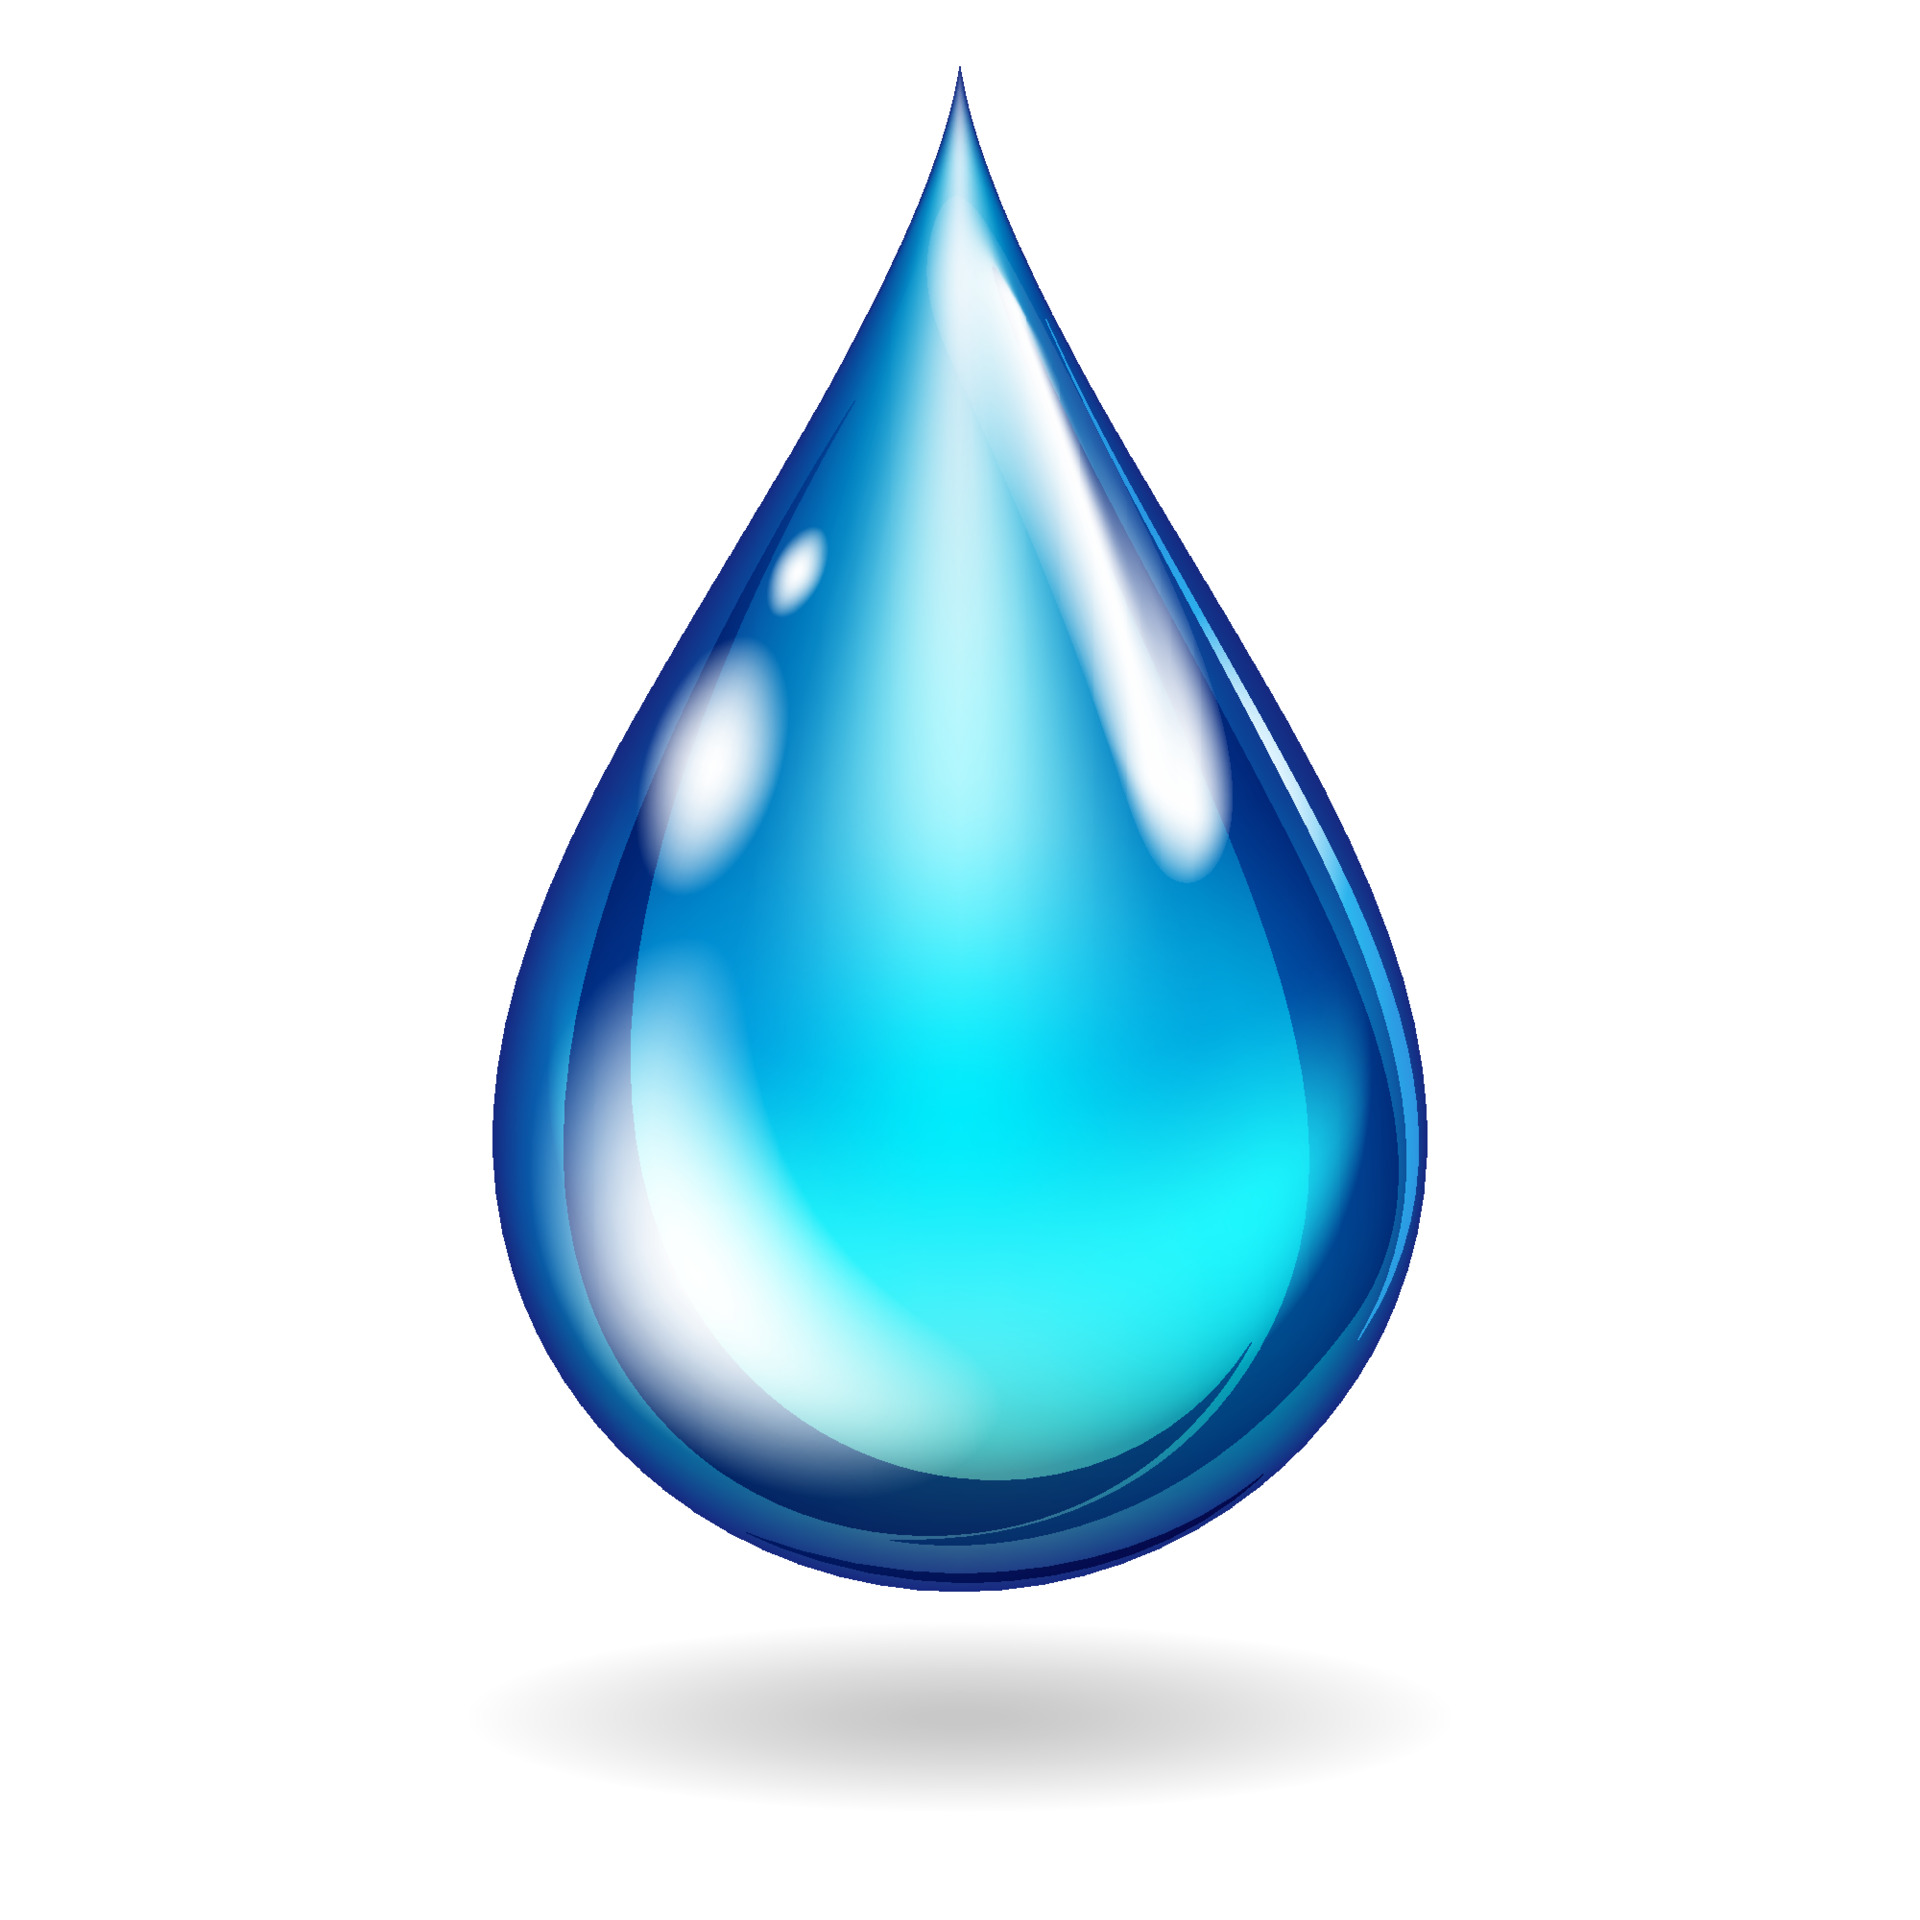
\includegraphics[scale=0.03, angle=0]{waterdrop.jpg}};
%
%\draw (current page.center)node [fill=blue!1!white!10,fill opacity=.003,text opacity=1,inner sep=2cm]at (7,2){ \Huge\centering\bfseries\sffamily\parbox[c][][t]{\paperwidth}{\centering \textcolor{Bittersweet}{} \\\vspace{3cm}\textcolor{BurntOrange}{Drinking Water Treatment \& Distribution}\\[15pt] % Book title
%% {\Large A Profound Subtitle}\\[20pt] % Subtitle
%{}}}; % Author name
\end{tikzpicture}
%\begin{center}
%
\includegraphics[scale=1, angle=-90]{BassettCTCLogo1.png} 
%\end{center}












%\begin{tikzpicture}[]
%\path[help lines,step=.2] (0,0) grid (16,6);
%\path[help lines,line width=.6pt,step=1] (0,0) grid (16,6);
%
%\node[inner sep=0pt] (background) at (current page.center) {\includegraphics[width=\paperwidth]{WaterBackground1.png}};
%\draw (current page.center)node [fill=blue!1!white!10,fill opacity=.3,text opacity=1,inner sep=2cm] { \Huge\centering\bfseries\sffamily\parbox[c][][t]{\paperwidth}{\centering \textcolor{Bittersweet}{October 2022} \\\textcolor{BurntOrange}{Drinking Water Treatment}\\[15pt]
%
%  \pgftext{
\includegraphics[width=300pt, angle =-90]{BassettCTCLogo1.png}} at (16,5);
%%  \pgftext{\includegraphics[width=150pt]{pic2.png}} at (0,0);
%\end{tikzpicture}
\vfill
\endgroup

%----------------------------------------------------------------------------------------
%	COPYRIGHT PAGE
%----------------------------------------------------------------------------------------

\newpage
~\vfill
\thispagestyle{empty}

%\noindent Copyright \copyright\ 2022 Shabbir Basrai\\ % Copyright notice
%
%\noindent \textsc{Published by Publisher}\\ % Publisher
%
%\noindent \textsc{book-website.com}\\ % URL
%
%\noindent Licensed under the Creative Commons Attribution-NonCommercial 3.0 Unported License (the ``License''). You may not use this file except in compliance with the License. You may obtain a copy of the License at \url{http://creativecommons.org/licenses/by-nc/3.0}. Unless required by applicable law or agreed to in writing, software distributed under the License is distributed on an \textsc{``as is'' basis, without warranties or conditions of any kind}, either express or implied. See the License for the specific language governing permissions and limitations under the License.\\ % License information, replace this with your own license (if any)

\noindent \textit{Revision Date: May 2023} % Printing/edition date

%----------------------------------------------------------------------------------------
%	TABLE OF CONTENTS
%----------------------------------------------------------------------------------------

%\usechapterimagefalse % If you don't want to include a chapter image, use this to toggle images off - it can be enabled later with \usechapterimagetrue

\chapterimage{TOCImage} % Table of contents heading image

\pagestyle{empty} % Disable headers and footers for the following pages

\tableofcontents % Print the table of contents itself
\listoffigures
\listoftables
\cleardoublepage % Forces the first chapter to start on an odd page so it's on the right side of the book

\pagestyle{fancy} % Enable headers and footers again

%----------------------------------------------------------------------------------------
%	PART
%----------------------------------------------------------------------------------------



%----------------------------------------------------------------------------------------
%	CHAPTER 1
%----------------------------------------------------------------------------------------

% \chapterimage{chapter_head_2.pdf} % Chapter heading image

% \chapter{Text Chapter}

% \section{Paragraphs of Text}\index{Paragraphs of Text}



% \lipsum[1-7] % Dummy text
% 
%------------------------------------------------

%\section{Citation}\index{Citation}
%
%This statement requires citation \cite{article_key}; this one is more specific \cite[162]{book_key}.

%------------------------------------------------

%\section{Lists}\index{Lists}
%
%Lists are useful to present information in a concise and/or ordered way\footnote{Footnote example...}.
%
%\subsection{Numbered List}\index{Lists!Numbered List}
%
%\begin{enumerate}
%\item The first item
%\item The second item
%\item The third item
%\end{enumerate}
%
%\subsection{Bullet Points}\index{Lists!Bullet Points}
%
%\begin{itemize}
%\item The first item
%\item The second item
%\item The third item
%\end{itemize}
%
%\subsection{Descriptions and Definitions}\index{Lists!Descriptions and Definitions}
%
%\begin{description}
%\item[Name] Description
+%\item[Word] Definition
%\item[Comment] Elaboration
%\end{description}1


%----------------------------------------------------------------------------------------
%	PART 2
%----------------------------------------------------------------------------------------


%----------------------------------------------------------------------------------------
%	CHAPTER 1
%----------------------------------------------------------------------------------------

%\chapter{Wastewater Math}
%
%\part{Module 1}
%\chapterimage{CertificationCover}
\chapter{Water Systems Operator Certifications}\index{Operator license!Water systems operator certifications}
\section{Operator certification background}\index{Operator certification background}
\begin{itemize}
\item Federal law requires operators at water treatment plants for drinking water, wastewater, and recycled water, as well as those involved in the distribution of drinking water, to be State certified.  

\item For drinking water, California's State Water Resources Control Board's (SWRCB's) Drinking Water Operator Certification Program (DWOPCP) under its Drinking Water Operator Certification Program (DWOCP), is responsible for the testing and certification of water treatment and water distribution operators throughout the state of California.

\item For wastewater, the SWRCB's Wastewater Operator Certification program (WWOCP) administers Wastewater Treatment Plant Certification examinations, certifications (Grades I to V), and certification renewals.

\item The CA-NV AWWA currently offers voluntary Advanced Water Treatment Operator (AWTO) certifications for water and wastewater operators to meet the high demand for highly skilled and certified advanced water treatment operators.

\end{itemize}

\section{Operational activities}\index{Operator!Operational activities}
California laws stipulate that water systems shall utilize only certified operators to make decisions addressing the following operational activities:\\
\subsection{Drinking water treatment:}\index{Operator!Operational activities!Treatment}
Water treatment operators work in water treatment plants where water from wells, rivers, streams, and reservoirs is treated and distributed to customers. Water treatment plant operators typically do the following:
\begin{itemize}
\item Add chemicals, such as ammonia, chlorine, or lime, to disinfect water or other liquids.
\item Inspect equipment on a regular basis.
\item Monitor operating conditions, meters, and gauges.
\item Collect and test water and sewage samples.
\item Record meter and gauge readings, and operational data.
\item Operate equipment to purify and clarify water, or to process or dispose of sewage.
\item Clean and maintain equipment, tanks, filter beds, and other work areas.
\item Stay current on environmental laws and regulations.
\item Ensure safety standards are met.
\end{itemize}
\subsection{Water distribution:}\index{Operator!Operational activities!Distribution}
\begin{itemize}
\item Water distribution operators are responsible for the safe and efficient operation of water pumps, valves, and other equipment. They monitor gauges and meters to ensure that water is being distributed in a timely manner and at appropriate pressures.

\item Water distribution operators may also be tasked with maintaining or repairing any equipment that breaks down during their shift. This could include anything from replacing parts on pumps to fixing leaks in pipes or hoses.
\item Water distribution operators typically do the following:
\begin{itemize}
\item Install, tap, re-line, disinfect, test and connect water mains and appurtenances.
\item Shutdown, repair, disinfect and test broken water mains.
\item Oversee the flushing, cleaning, and pigging of existing water mains.
\item Pull, reset, rehabilitate, disinfect and test domestic water wells.
\item Stand-by emergency response duties for after hours distribution system operational emergencies.
\item Drain, clean, disinfect, and maintain distribution reservoirs.
\end{itemize}
\end{itemize}
Water systems shall utilize either certified distribution operators or treatment operators that have been trained to make decisions addressing the following operational activities:\\
\begin{itemize}
\item Operate pumps and related flow and pressure control and storage facilities manually or by using a system control and data acquisition (SCADA) system.
\item Maintain and/or adjust system flow and pressure requirements, control flows to meet consumer demands.
\item Determine and control proper chemical dosage rates for wellhead disinfection and distribution residual maintenance.
\item Investigate water quality problems in the distribution system.
\end{itemize}


\subsection{Wastewater treatment:}\index{Operator!Operational activities!Wastewater}
Wastewater operators typically do the following as part of their job responsibilities:
\begin{itemize}
\item Operate and maintain the wastewater treatment plant and collection systems.
\item Operate and adjust controls on treatment plant equipment and machinery, such as valves, pumps, and motors. 
\item Read and interpret meters and gauges.
\item Regulate plant effluent.
\item Monitor, repair, and maintain wastewater system lift stations; remove debris; disassemble and clean pumps; perform minor repairs when necessary. Locate problems and operate sewer cleaning equipment to clear blockages.
\item Performs routine maintenance and minor repairs on plant equipment, system equipment,
facilities, distribution system, and collection system.
\item Maintaining plant records and preparing monthly and quarterly reports.
\item Perform all aspects of sampling, monitoring, and testing required to maintain compliance with Federal, State, and Local regulations governing the wastewater treatment process, stormwater, and sludge management.
\end{itemize}

\subsection{Advanced treatment/water reuse:}\index{Operator!Operational activities!Advanced treatment/water reuse}
The Advanced Water Treatment Operators (AWTO) perform a full range of duties associated with operating and maintaining water treatment systems and equipment used for Advanced Water Treatment for water reuse.
AWTO typically do the following as part of their job responsibilities:\\
\begin{itemize}
\item Operate, monitor, and maintain AWT processes, such as membrane systems and advanced oxidation.
\item AWTOs have an advanced understanding of technologies and regulations pertinent to the end uses of treated water; such as recycled water, potable water, and potable water reuse.
\item At the supervisor and management level, maintain regular communication with regulatory agencies and ensure permit compliance. 
\item Responsibility for preparing and submitting regulatory reports.
\end{itemize}
\newpage
\section{Qualifications and eligibility}\index{Operator license!Qualifications and eligibility}
\subsection{Treatment}
\begin{table}[H]
\captionsetup{justification=centering}
\scriptsize

\begin{tabular}{|c|p{7.1cm}|p{7cm}|}
\hline
\thead{Grade} & \thead{Minimum Qualifications for Examination                                                                                                                                                                                                                                                                                     } & \thead{Eligibility Criteria for Certification                                                                                                                                                                                                                                                                                                                                                                                                                                                                                                } \\
\hline
T1    & High School Diploma / GED Equivalency*.                                                                                                                                                                                                                                                                                     & Successful completion of the Grade   T1 examination within the three years prior to   submitting certification application.                                                                                                                                                                                                                                                                                                                                                                                                            \\
\hline
T2    & \makecell[l]{High School Diploma / GED Equivalency*\\AND\\One 3-unit (or 36-hour) course of specialized training covering\\the fundamentals of drinking water treatment.} & \makecell[l]{Successful completion of the Grade T2 examination within\\the three years prior to submitting certification application.                                                                                                                                                                                                                                                                                                                                                                                                           } \\
\hline
T3    & \makecell[l]{High School Diploma / GED Equivalency*\\AND\\Two 3-unit (or 36-hour) courses of specialized training\\that include at least one course in drinking water treatment and a \\second course in either drinking water treatment, distribution,\\or wastewater treatment.}& \makecell[l]{Successful completion of the Grade T3 examination within the\\three years prior to   submitting certification application\\AND\\At least one year of operator experience working as a   certified\\T2 operator at a T2 facility or higher. This may be substituted\\with (3) below.\\AND\\      At least one additional year of operator experience working as a\\certified treatment operator. This may be substituted with\\(1), (2), or (4) below.}\\  
\hline                               
T4    & \makecell[l]{Current T3 certification\\AND\\Three 3-unit (or 36-hour) courses of specialized training that\\include at least two courses in the fundamentals of drinking\\water treatment and a third course in either\\drinking water treatment, distribution, or wastewater treatment.} & \makecell[l]{Successful completion of the Grade T4 examination within the\\three years prior to submitting the certification application\\AND\\At least one year of operator experience working as shift\\or chief operator, while a certified T3 operator at a T3\\facility or   higher. This may be substituted with (3) below.\\AND\\At least three additional years of operator experience\\working as a certified treatment operator. This may be\\substituted with (1) or (4) below.}\\
\hline
T5    & \makecell[l]{Current T4 certification\\AND\\Four 3-unit (or 36-hour) courses of specialized training that\\include\\at least two courses in drinking water treatment and two \\additional   courses in either drinking water treatment, \\distribution,or wastewater   treatment.}              & \makecell[l]{Successful completion of the Grade T5 examination within the\\three years prior to   submitting the application for certification\\AND\\At least two years of operator experience working as a   shift or\\chief operator, while a certified T4 operator at a T4 facility or \\ higher. There are no substitutions.\\AND\\At least three additional years of operator experience working\\ as a  certified treatment operator. This may be substituted with\\(1) or (4) below.} \\ 
\hline      
\end{tabular}
\caption{Water treatment license Exams - qualifications and eligibility}
\end{table}
\begin{tiny}
High School Diploma/GED equivalency for Grades 1 and 2 ONLY can be fulfilled with either successful completion of Basic Small Water Systems Operations course provided by the Department
OR 1 year as an operator of a facility that required an understanding of a chemical feeds, hydraulic systems, and pumps."\\			
Experience substitutions for certification, as referenced above.
\begin{enumerate}
\item A relevant degree earned at an accredited academic institution may be substituted as follows:
\begin{enumerate}[label=\alph*)]
\item Associate’s Degree or Certificate in Water or Wastewater Technology that includes at least 15 units of physical, chemical, or biological science may be used to fulfill 1 year of operator experience.
\item Bachelor’s Degree in engineering or in physical, chemical, or biological sciences (e.g Biology, Chemical Engineering, Chemistry, Civil Engineering, Environmental Engineering, Microbiology, Public Health, or Sanitary Engineering) may be used to fulfill 1.5 years of operator experience.
\item Master’s Degree in the above mentioned fields in (b) may be used to fulfill 2 years of operator experience.
\end{enumerate}
\item A certified operator may substitute, on a day-for-day basis, experience gained while working with lead responsibility for water quality related projects of research.
\item If an applicant has a Bachelor’s or Master’s of Science degree, completion of a comprehensive operator training program, may be substituted for the required experience.
\item Experience gained as a certified wastewater treatment operator may be used to substitute up to 2 years of the experience requirement. Wastewater treatment operator experience is credited on a two-for-one basis (i.e. 2 months in wastewater=1 month in drinking water).		
\end{enumerate}
\end{tiny}
\newpage
\subsection{Distribution}

\begin{table}[H]
\captionsetup{justification=centering}
\scriptsize

%\tiny, \scriptsize, \footnotesize, \small, \normalsize, \large, \Large, \LARGE, \huge, and \Huge.
\begin{tabular}{|c|p{7.1cm}|p{7cm}|}
\hline
\thead{Grade} & \thead{Minimum Qualifications for\\ Examination                                                                                                                                                                                                                                                                                            } & \thead{Eligibility Criteria for\\ Certification                                                                                                                                                                                                                                                                                                                                                                                                                      } \\ \hline


D1    & High School Diploma / GED Equivalency*                                                                                                                                                                                                                                                                                             & \makecell[l]{Successful completion of the Grade   D1 examination within \\the three years prior to\\submitting certification application.                                                                                                                                                                                                                                                                                                                                 } \\ 
\hline


D2    & \makecell[l]{High School Diploma / GED Equivalency*\\ AND\\ One 3-unit (or 36-hour) course of specialized training covering\\the fundamentals of water supply principles.} & \makecell[l]{Successful completion of the Grade D2 examination within \\the three years prior to submitting certification \\application}.                                                                                                                                                                                                                                                                                                                                \\ 
\hline


D3    & \makecell[l]{Current D2 Certification\\AND\\Two 3-unit (or 36-hour) courses of specialized training that\\includes at least one course in the fundamentals of water supply\\ principles and a second course in either drinking water\\distribution, treatment, or   wastewater treatment.} & \makecell[l]{Successful completion of the Grade D3 examination within\\the three years prior to submitting certification application\\AND\\At least one year of operator experience working as a certified\\D2 operator for a D2 system or higher\\AND\\At least one additional year of operator experience working\\as a distribution operator. This may be substituted with (1)\\or (2) below.}\\ 
\hline


D4    & \makecell[l]{Current D3 certification\\ AND \\Three 3-unit (or 36-hour) courses of specialized training\\that includes at least two courses in the fundamentals of water supply\\ principles and a third course in either drinking water distribution,\\treatment, or wastewater treatment.}& \makecell[l]{Successful completion of the Grade   D4 examination within the \\three years prior to submitting the application for certification\\ AND\\ At least one year of operator experience working as a\\certified D3 operator for a D3 system or higher\\ AND\\ At least three additional years of operator experience working\\as a distribution operator. This may be substituted with (1)\\or (2) below.}\\ \hline
D5    & \makecell[l]{Current D4 certification\\AND\\Four 3-unit (or 36-hour) courses of specialized training\\ that includes at least two courses in the fundamentals of water\\supply principles and two additional courses in either\\ drinking water distribution, treatment, or wastewater treatment.} & \makecell[l]{Successful completion of the Grade D5 examination within\\the three years prior to submitting the application for\\certification\\AND\\At least two years of operator experience working as a\\certified D4 operator for a D4 or D5 system\\AND\\At least three additional years of operator experience\\working as a distribution operator. This may be substituted\\with (1) or (2) below.}\\ \hline
\end{tabular}
\caption{Distribution license exams - qualifications and eligibility}
\end{table}

\begin{tiny}

High School Diploma/GED equivalency for Grades 1 and 2 ONLY can be fulfilled with either successful completion of Basic Small Water Systems Operations course provided by the Department OR 1 year as an operator of a facility that required an understanding of a piping system that included pumps, valves, and storage tanks.\\

Experience substitutions for certification, as referenced above.
\begin{enumerate}[]
\item A relevant degree earned at an accredited academic institution may be substituted as follows:
\begin{enumerate}[label=(\alph*)]
\item Associate’s Degree or Certificate in Water or Wastewater Technology that includes at least 15 units of physical, chemical, or biological science may be used to fulfill 1 year of operator experience.
\item Bachelor’s Degree in engineering or in physical, chemical, or biological sciences (e.g. Biology, Chemical Engineering, Chemistry, Civil Engineering, Environmental Engineering, Microbiology, Public Health, or Sanitary Engineering) may be used to fulfill 1.5 years of operator experience.
\item Master’s Degree in the above mentioned fields in (b) may be used to fulfill 2 years of operator experience.
\end{enumerate}
\item A certified operator may substitute, on a day-for-day basis, 1 additional year of operator experience working as a distribution operator with experience gained while working with lead responsibility for water quality or quantity related projects or research.
\end{enumerate}	
\end{tiny}

\newpage
\subsection{Wastewater}
\begin{table}[H]
\captionsetup{justification=centering}
\scriptsize
\begin{tabular}{|l|p{6.5cm}|l|p{6.5cm}|}
\hline

\multicolumn{1}{|c|}{\thead{PATH}} & 
  \multicolumn{1}{|c|}{\thead{EXAMINATION EDUCATION REQUIREMENTS}} & &\multicolumn{1}{|c|}{\thead{CERTIFICATION QUALIFYING EXPERIENCE \\REQUIREMENTS}}\\\hline


%\thead{PATH} & \thead{EXAMINATION EDUCATION REQUIREMENTS}&     &\thead{CERTIFICATION QUALIFYING EXPERIENCE \\REQUIREMENTS}\\ \hline
GRADE I   &                                                                                                                                                                                                                                                                                               &     &                                                                                                 \\ \hline
1         & High  school  diploma or equivalent and 6 educational pts                                                                                                                                                                                                                          & and & 1 year of full-time qualifying experience                                   \\ \hline
GRADE II  &                                                                                                                                                                                                                                                                                               &     &                                                                                                 \\ \hline
1         & High  school  diploma    or  equivalent  and    9 educational pts                                                                                                                                                                                                                          & and & 18   months   of     full-time   qualifying   experience as a Grade I operator                  \\ \hline
2         & High  school  diploma    or  equivalent  and    12 educational pts                                                                                                                                                                                                                         & and & 2    years    of      full-time    qualifying   experience                                      \\ \hline
3         & \makecell[l]{Associate’s  degree,  a    higher  degree,  or  a minimum   of\\   60  college   semester   units, including a minimum of 15\\semester units of science courses                                                                                                                          } & and & 1     year     of       full-time     qualifying   experience                                   \\ \hline
GRADE III &                                                                                                                                                                                                                                                                                               &     &                                                                                                 \\ \hline
1         & High  school  diploma    or  equivalent  and    12 educational pts                                                                                                                                                                                                                         & and & 3    years    of      full-time    qualifying   experience as a Grade II operator               \\ \hline
2         & High  school  diploma    or  equivalent  and    18 educational pts                                                                                                                                                                                                                         & and & 4    years    of      full-time    qualifying   experience                                      \\ \hline
3         & \makecell[l]{Associate’s  degree  or    a  minimum   of     60 college semester\\ units,including a minimum of 15 semester units of\\science courses                                                                                                                                                      } & and & 2    years    of      full-time    qualifying   experience                                      \\ \hline
4         & \makecell[l]{Bachelor’s   degree   or     a   higher   degree, including a\\ minimum of 30 semester   units of science courses                                                                                                                                                                              } & and & 1     year     of       full-time     qualifying   experience                                   \\ \hline
GRADE IV  &                                                                                                                                                                                                                                                                                               &     &                                                                                                 \\ \hline
1         & High  school  diploma    or  equivalent  and    32 educational points                                                                                                                                                                                                                         & and & 6    years    of      full-time    qualifying   experience                                      \\ \hline
2         & \makecell[l]{Associate’s   degree   or     a  minimum   of     60 college semester \\units, including a minimum of 15 semester units of   science\\ courses                                                                                                                                                   } & and & 4    years    of      full-time    qualifying   experience                                      \\ \hline
3         & \makecell[l]{Bachelor’s   degree   or     a   higher   degree, including a minimum\\ of 30 semester   units of science courses                                                                                                                                                                              } & and & 3    years    of      full-time    qualifying   experience                                      \\ \hline
4         &\makecell[l]{ Valid  registration  as    a  chemical,  civil,\\or mechanical     engineer     issued     by the California  Board \\ for    Professional  Engineers and  Land    Surveyors  or  by\\ another  state, territory, or   Indian tribe                                                   } & and & 2    years    of      full-time    qualifying   experience                                      \\ \hline
GRADE V   &                                                                                                                                                                                                                                                                                               &     &                                                                                                 \\ \hline
1         & High  school  diploma    or  equivalent  and    48 educational points                                                                                                                                                                                                                         & and & 10      years      full-time      qualifying experience                                         \\ \hline
2         & \makecell[l]{Associate’s   degree   or     a  minimum   of     60 college semester \\units, including a minimum of 15 semester units of   science\\courses                                                                                                                                                   } & and & 6    years    of      full-time    qualifying   experience                                      \\ \hline
3         & Bachelor’s   degree   or     a   higher   degree, including a minimum of 30 semester   units of science courses                                                                                                                                                                               & and & 5    years    of      full-time    qualifying   experience                                      \\ \hline
4         & \makecell[l]{Valid  registration  as    a  chemical,  civil,    or mechanical\\ engineer issued by the California  Board  for    Professional\\  Engineers and Land    Surveyors or  by another  state,  a \\territory, or an Indian tribe} & and & 4    years    of      full-time    qualifying   experience                                      \\ \hline
\end{tabular}
\caption{Wastewater operator license exams requirements}
\end{table}

\begin{itemize}
\scriptsize
\item 1,800 hours of qualifying experience as an Operator-In-Training (OIT) \index{Operator-in-training (OIT)} at a wastewater treatment plant (WWTP) is required to become a certified operator. The 1,800 OIT hours counts as one year of full-time qualifying experience.
\item OIT applicants must submit a copy of a high school diploma or equivalent and six educational points.
\item Volunteer, part-time, full-time and overtime hours qualify.
\item OIT hours are not grade level specific and OIT experience does NOT expire.
\item OIT certificates are good for three years from the date of issuance and can be renewed.  To renew an OIT certificate, an applicant must have taken and passed a Wastewater Exam within the last four years.
\end{itemize}
\newpage
\subsection{Advanced water treatment or water reuse}
\begin{table}[H]
\captionsetup{justification=centering}
\scriptsize
\begin{tabularx}{\textwidth}{| X | X |}
%{
%|>{\setlength\hsize{1.\hsize}\setlength\linewidth{\hsize}}X|
%>{\setlength\hsize{.5\hsize}\setlength\linewidth{\hsize}}X|
%>{\setlength\hsize{.01\hsize}\setlength\linewidth{\hsize}}X|}

\hline
\multicolumn{2}{|l|}{Grade 3}                                                                                                                                                                                                                                                                                                                                                                                                   \\
\hline
\begin{itemize}
\item Possess a current state issued Drinking Water Treatment Operator Certification or Wastewater Treatment Plant   Operator Certification, Grade III or higher                                                                                                                                                                                             
\end{itemize} & 
\begin{itemize}
\item Successful completion of AWTO Grade 3 Exam (AWT3TM)
\end{itemize} \\
\hline
\multicolumn{2}{|l|}{Grade 4}                                                                                                                                                                                                                                                                                                                                                                                                   \\
\hline
\begin{itemize}
\item Possess a current AWT3 certification
\item 2 years of   experience with one or more AWT processes (see Table 1). Retroactive   experience prior to AWT3 certification may be included 
\end{itemize}
& 
\begin{itemize}
\item Successful   completion of AWTO Grade 4 Exam (AWT4TM) 
\end{itemize}\\
\hline
\multicolumn{2}{|l|}{Grade 5}                                                                                                                                                                                                                                                                                                                                                                                                  \\
\hline
\begin{itemize} 
\item Possess a   current AWT4 certification 
\item 3 years of   experience to include 2 years of experience in at least one AWT process and 1   additional year with at least 2 AWT processes in a single treatment train   (see Table 1). Retroactive experience prior to AWT4 certification may be   included. 
\end{itemize}
&\begin{itemize}
\item Successful completion of AWTO Grade 5 Exam (AWT5TM)
\end{itemize}\\
\hline
\end{tabularx}

\caption{Advanced water treatment certification requirements}
\end{table}
\begin{table}[H]
\captionsetup{justification=centering}
\scriptsize
\begin{center}
\begin{tabular}{|l|p{2cm}|p{2cm}|p{2cm}|}
\hline
 & \begin{center}  {Exam Fee} \end{center} & \begin{center}{Reexamination Fee}  \end{center} & \begin{center}{Application Fee}  \end{center}\\
\hline
D1 \& T1 & \multicolumn{1}{|c|}{\$50} & \multicolumn{1}{|c|}{ \$30} & \multicolumn{1}{|c|}{\$70}\\
\hline
D2 \& T2  & \multicolumn{1}{|c|}{\$65} & \multicolumn{1}{|c|}{\$45} & \multicolumn{1}{|c|}{\$80}\\
\hline
D3 \& T3 & \multicolumn{1}{|c|}{\$100} & \multicolumn{1}{|c|}{\$70} & \multicolumn{1}{|c|}{\$120}\\
\hline
D4 \& T4 & \multicolumn{1}{|c|}{\$130}& \multicolumn{1}{|c|}{\$95}& \multicolumn{1}{|c|}{\$140}\\
\hline
D5 \& T5 & \multicolumn{1}{|c|}{\$155}& \multicolumn{1}{|c|}{\$120}& \multicolumn{1}{|c|}{\$140}\\
\hline
WW Grade I & \multicolumn{1}{|c|}{\$50} & \multicolumn{1}{|c|}{ \$30} & \multicolumn{1}{|c|}{\$95}\\
\hline
WW Grade II  & \multicolumn{1}{|c|}{\$65} & \multicolumn{1}{|c|}{\$45} & \multicolumn{1}{|c|}{\$125}\\
\hline
WW Grade III  & \multicolumn{1}{|c|}{\$100} & \multicolumn{1}{|c|}{\$70} & \multicolumn{1}{|c|}{\$170}\\
\hline
WW Grade IV & \multicolumn{1}{|c|}{\$130}& \multicolumn{1}{|c|}{\$95}& \multicolumn{1}{|c|}{\$190}\\
\hline
WW Grade V  & \multicolumn{1}{|c|}{\$155}& \multicolumn{1}{|c|}{\$120}& \multicolumn{1}{|c|}{\$190}\\
\hline
\multirow{2}{*}{AWWA - AWTO Grades III - V} & \multicolumn{3}{|l|}{\$250 - for Members of CA-NV AWWA, CWEA or both} \\
&\multicolumn{3}{|l|}{\$350 - for Non-Members of either association}\\
\hline
\end{tabular}
\caption{Exam and application fees}
\end{center}
\end{table}
\section{Expected range of knowledge}
\subsection{Treatment}
The Expected Range of Knowledge for Drinking Water Treatment Exam is provided in Appendix \ref{appendix:Treatment Exam - ROK}.\\
\subsection{Distribution}
The Expected Range of Knowledge for Drinking Water Distribution Exam is provided in Appendix \ref{appendix:Distribution Exam - ROK}.\\
\subsection{Wastewater}
Details for each of the Grades I-V Wastewater Operator License Exams is provided in Appendix \ref{appendix:Wastewater Exams}.\\
\section{Certification requirements}\index{Water Operator!certification requirements}
\subsection{Treatment}
\begin{itemize} 
\item Treatment systems are classified as T1-T5, according to a point system that takes into account various source water characteristics, maximum capacity and treatment techniques. Appendix \ref{appendix:Water Treatment Facilities Classification} provides details on the classification of water treatment facilities.\\
\begin{table}[H]
\begin{center}
\captionsetup{justification=centering}
\begin{tabular}{|l|c|}
\hline
Total Points & Class\\
\hline
Less than 20 & T1\\
\hline
20 through 39 & T2\\
\hline
40 through 59&  T3\\
\hline
60 through 79 & T4\\
\hline
80 or more & T5\\
\hline
\end{tabular}
\caption{Water treatment facility class designations}
\end{center}
\end{table}

\item Any person operating a water treatment plant is required to possess a valid, unexpired water treatment operator certificate of appropriate grade.

\item The certification requirements of the Chief Treatment Plant Operator and that of the Shift Operator - persons  in responsible charge of the water treatment plant,  are required to possess a valid, unexpired water treatment operator certificate equal to or greater than the classification of the water treatment plant.

\begin{table}[H]
\begin{center}
\begin{tabular}{|c|c|c|}
\hline
\begin{tabular}{c}
Total Points \\
Class \\
\end{tabular} & \begin{tabular}{c}
Minimum Certification of \\
Chief Operator \\
\end{tabular} & \begin{tabular}{c}
Minimum Certification \\
of Shift Operator \\
\end{tabular} \\
\hline
T1 & T1 & T1 \\
\hline
T2 & T2 & T1 \\
\hline
T3 & T3 & T2 \\
\hline
T4 & T4 & T3 \\
\hline
T5 & T5 & T3 \\
\hline
\end{tabular}
\caption{Minimum certification requirements for Chief and Shift Operators}\index{Minimum certification requirements for treatment plants' chief and shift operators}
\end{center}
\end{table}
\end{itemize}
\newpage
\subsection{Distribution}
\begin{itemize}
\item Distribution systems are classified as D1 to D5 by population served and system complexity. The population categories are:\\
\begin{table}[H]
\begin{center}
\captionsetup{justification=centering}
\begin{tabular}{|l|c|}
\hline
\textbf{Class} & \textbf{Population Served} \\
\hline
D1 & $\leq$1,000\\
\hline
D2 & 1,001 - 10,000\\
\hline
D3 &  10,001 - 50,000\\
\hline
D4 & 50,001 - 5 million\\
\hline
D5 & $\geq$5 million\\
\hline
\end{tabular}
\caption{Distribution systems class designations}
\end{center}
\end{table} 
\item Distribution systems can be upgraded one level due to complexity, using a point system which takes into account: number of pressure zones, storage reservoirs and uncovered storage reservoirs, treatment, the size of the largest pump utilized, and customers with a nonpotable water supply connection. 
\item A person who operates a water distribution system shall possess a valid, unexpired water distribution operator certificate of the appropriate grade in accordance with the regulations.
\item  A person who is in responsible charge of the water distribution system shall possess a valid, unexpired water distribution operator certificate equal to or greater than the classification of the water distribution system.
\end{itemize}
\begin{table}[H]
\begin{center}
\begin{tabular}{|c|c|c|}
\hline
\begin{tabular}{c}
\textbf{Distribution System} \\
\textbf{Classification} \\
\end{tabular} & \begin{tabular}{c}
\textbf{Minimum Certification of} \\
\textbf{Chief Operator} \\
\end{tabular} & \begin{tabular}{c}
\textbf{Minimum Certification} \\
\textbf{of Shift Operator} \\
\end{tabular} \\
\hline
D1 & D1 & D1 \\
\hline
D2 & D2 & D1 \\
\hline
D3 & D3 & D2 \\
\hline
D4 & D4 & D3 \\
\hline
D5 & D5 & D3 \\
\hline
\end{tabular}
\caption{Minimum certification requirements for Chief and Shift Operators}\index{Minimum certification requirements for distribution systems' chief and shift operators}
\end{center}
\end{table}
\newpage
\subsection{Wastewater}
\begin{itemize}
\item All wastewater plant operators are required to possess at least a valid Grade I certificate, a valid provisional operator certificate, or a valid operator-in-training certificate.
\item Wastewater treatment plants are classified as Class I to V based upon the plant design flow and treatment process. 
\begin{table}[H]
\begin{center}
\begin{tabular}{|c|l|l|}
\hline
{\textbf{Class} }                    & \multicolumn{1}{c|}{ \textbf{Treatment Process}} & \multicolumn{1}{c|}{\textbf{Design Flow (MGD)}} \\ \hline
\multirow{2}{*}{I}                       & Pond                                                  & All                                                   \\ \cline{2-3} 
                                         & Primary                                               & 1 or less                                           \\ \hline
\multirow{3}{*}{II}                      & Primary                                               & Greater than 1 through 5                          \\ \cline{2-3} 
                                         & Biofiltration                                         & 1 or less                                           \\ \cline{2-3} 
                                         & Extended Aeration                                     & All                                                   \\ \hline
\multirow{4}{*}{III}                     & Primary                                               & Greater than 5 through 20                         \\ \cline{2-3} 
                                         & Biofiltration                                         & Greater than 1 through 10                         \\ \cline{2-3} 
                                         & Activated Sludge                                      & 5 or less                                           \\ \cline{2-3} 
                                         & Tertiary                                              & 1 or less                                           \\ \hline
\multirow{4}{*}{IV}                      & Primary                                               & Greater than 20                                     \\ \cline{2-3} 
                                         & Biofiltration                                         & Greater than 10 through 30                        \\ \cline{2-3} 
                                         & Activated Sludge                                      & Greater than 5 through 20                         \\ \cline{2-3} 
                                         & Tertiary                                              & Greater than 1 through 10                         \\ \hline
\multicolumn{1}{|l|}{\multirow{3}{*}{V}} & Biofiltration                                         & Greater than 30                                     \\ \cline{2-3} 
\multicolumn{1}{|l|}{}                   & Activated Sludge                                      & Greater than 20                                     \\ \cline{2-3} 
\multicolumn{1}{|l|}{}                   & Tertiary                                              & Greater than 10                                     \\ \hline
\end{tabular}
\caption{Wastewater treatment plant classification}\label{Wastewater treatment plant classification}\index{Wastewater treatment plant classification}
\end{center}
\end{table}
\item For each plant class, WWOCP sipulates that the Chief plant operator and designated operator-in- charge shall possess a valid operator certificate at a grade level at least equivalent as provided to the following: 
\end{itemize}
\begin{table}[H]
\begin{center}
\begin{tabular}{|c|c|c|}
\hline
\begin{tabular}{c}
Wastewater \\
Treatment Plant \\
Classification \\
\end{tabular} & \begin{tabular}{c}
Minimum Grade Level of \\
Chief Plant Operator \\
\end{tabular} & \begin{tabular}{c}
Minimum Grade Level of \\
Designated Operator-in-Charge \\
\end{tabular} \\
\hline
I & I & I \\
\hline
II & II & I \\
\hline
III & III & II \\
\hline
IV & IV & III \\
\hline
\end{tabular}
\end{center}
\end{table}
\newpage
\subsection{Advanced water treatment}
\begin{itemize}
\item Per California laws, a water treatment plant operator may operate a water recycling treatment plant at a grade level appropriate for the class of wastewater treatment plant being operated.
 \begin{table}[H]
\begin{center}
\begin{tabular}{|c|c|c|}
\hline
\begin{tabular}{c}
Wastewater Treatment \\
Plant Classification \\
\end{tabular} & \begin{tabular}{c}
Water Treatment Plant \\
Operator Certificate \\
\end{tabular} & \begin{tabular}{c}
Wastewater Treatment Plant \\
Operator Certificate \\
\end{tabular} \\
\hline
I & T1 & Grade I \\
\hline
II & T2 & Grade II \\
\hline
III & T3 & Grade III \\
\hline
IV & T4 & Grade IV \\
\hline
V & T5 & Grade V \\
\hline
\end{tabular}
\caption{Certificate requirements for water recycling treatment plants}
\end{center}
\end{table}
\end{itemize}
\section{Certification renewal}\index{Water Operator!Certification renewal}
\begin{itemize}
\item Certification must be renewed every 3 years, or at least 120 days, but not more than 180 days, before the expiration date. 
\item Operators are expected to complete required number of continuing education contact hours during their renewal period. The continuing education requirements to renew a California water operator certificate are as follows:  \\
\item Continuing education are courses, classes or seminars that present “information related to the operation of a drinking water treatment facility and/or distribution system.”  Continuing education hours can be earned by attending water industry 
meetings, conferences, workshops, in-­house training, college courses, correspondence 
courses and internet classes.
\item There are no continuing education requirements for wastewater operator certification renewal. 
\end{itemize}
\begin{table}[H]
\begin{center}
\begin{tabular}{|p{2cm}|p{8cm}|}
\hline

\begin{center}{\textbf{Exam}}\end{center} & \begin{center}{\textbf{Required Continuing Education Contact Hours}}\end{center}\\
\hline
D1, T1 & 12 hours\\
\hline
D2, T2 & 16 hours\\
\hline
D3, T3 & 24 hours\\
\hline
D4, T4 & 36 hours\\
\hline
D5, T5 & 36 hours\\
\hline
\multicolumn{2}{|l|}{Up to 25\% of contact hours can be fulfilled by completing safety training.}\\
\hline
\end{tabular}
\caption{Certificate renewal contact hours requirements}
\end{center}
\end{table}
\newpage
\begin{table}[ht!]
\captionsetup{justification=centering}
\scriptsize
\begin{center}
\begin{tabular}{|c|p{2cm}|p{2cm}|}
\hline
 & \begin{center}{Triennial renewal}\end{center} & \begin{center}{Discounted certification and renewal}\end{center}\\
\hline
D1 \& T1 & \multicolumn{1}{|c|}{\$70} & \multicolumn{1}{|c|}{\$55$^1$}\\
\hline
D2 \& T2  & \multicolumn{1}{|c|}{\$80} & \multicolumn{1}{|c|}{\$60$^1$}\\
\hline
D3 \& T3 & \multicolumn{1}{|c|}{\$120} & \multicolumn{1}{|c|}{\$90$^1$}\\
\hline
D4 \& T4 & \multicolumn{1}{|c|}{\$140}& \multicolumn{1}{|c|}{\$105$^1$}\\
\hline
D5 \& T5 &  \multicolumn{1}{|c|}{\$140}& \multicolumn{1}{|c|}{\$105$^1$}\\
\hline
WW Grades I - V & \multicolumn{1}{|c|}{\$150}& \multicolumn{1}{|c|}{\$115$^2$}\\
\hline
\multicolumn{3}{|l|}{$^1$ For operators with both a water treatment and water }\\ \multicolumn{3}{|l|}{ \hspace{0.27cm}distribution certificates}\\
\multicolumn{3}{|l|}{$^2$ For operators with both a wastewater and water}\\ \multicolumn{3}{|l|}{   \hspace{0.27cm}treatment/distribution certificate}\\
\hline

\end{tabular}
\caption{Certificate renewal fees}
\end{center}
\end{table}








Which one of the following best defines the term aquifer?\\
A low lying area where water pools\\
Water-bearing stratum of rock, sand, or gravel\\
Impervious stratum near the ground surface\\
Treated water leaving the water system\\
The height to which water will rise in wells located in an artesian aquifer is called the\\
Pumping water level\\
Water table\\
Piezometric surface\\
Drawdown\\
Radius of influence\\
What percentage of all the earth's water is readily available as a potential drinking water supply in the form of lakes, rivers, and near-surface groundwater?\\
97\%\\
50\%\\
2\%\\
1\%\\
0.34\%\\
To  prevent the entry of surface contamination into a well is the purpose of\\
The well casing\\
The water table\\
The louvers or slots\\
Well development\\
The  annular grout seal	\\
An aquifer that is located underneath an aquiclude is called\\
An unconfined aquifer\\
A confined aquifer\\
A water table\\
Unreachable groundwater\\
An Artesian spring\\
The process by which water changes from the gas to the liquid phase is termed\\
Condensation	·\\
Evaporation\\
Percolation\\
Precipitation\\
Runoff\\
The free surface of the water in an unconfined aquifer is known as the\\
Pumping water level\\
Artesian spring\\
Water table\\
Drawdown\\
Percolation\\
The transfer of liquid water from plants and animals on the surface of the earth into water vapor in the atmosphere is called\\
Transpiration\\
Evaporation\\
Condensation\\
Runoff\\
Percolation\\
The elevation of water in the casing of an operating well is called the\\
Piezometric surface\\
Water table\\
Pumping water level\\
Drawdown\\
Radius of influence\\
An aquifer under pressure is often termed\\
Unconfined\\
Pacific\\
Artesian\\
Alluvial\\
Elevated\\
An aquifer is usually composed of\\
Sand and gravel \\
Clays and silts\\
Bedrock\\
Large voids in the soil, resembling underground lakes\\
None of the above\\
Which of the following best defines the term specific capacity?\\
Amount of water a given volume of saturated rock or sediment will yield to gravity\\
Amount of water a given volume of saturated rock or sediment will yield to pumping\\
Rate at which water would flow in an aquifer if the aquifer were an open conduit\\
Amount of water a well will produce for each foot of drawdown\\
The most common type of well used for public water supply systems is a\\
Jetted well\\
Driven well\\
Drilled well\\
Bored well\\
Which of the following best defines the term static water level?\\
Water level in a well after a pump has operated for a period of time\\
Water level in a well when the well is not in operation\\
Water level in a well measured from the ground surface to the drawdown water level\\
Waterlevel in a well measured from the natural water level to the drawdown water level\\
The residual drawdown of a well is defined as\\
Water level in a well after a pump has operated over a period of time\\
Measured distance from the ground to the pumping level\\
Water level below the normal level that persists after a well pump has been off for a period of time\\
Measured distance between the water level and the top of the screen\\
A well is located in an aquifer with a water table elevation 20 feet below the ground surface. After operating for three hours, the water level in the well stabilizes at 50 feet below the ground surface. The pumping water level is:\\
20 feet\\
30 feet\\
50 feet\\
70 feet\\
100 feet\\
What percentage of all the earth's water is readily available as a potential drinking water supply in the form of lakes, rivers, and near-surface groundwater?\\
97\%\\
50\%\\
2\%\\
1\%\\
0.34\%\\
To  prevent the entry of surface contamination into a well is the purpose of\\
The well casing\\
The water table\\
The louvers or slots\\
Well development\\
The  annular grout seal	\\
The process by which water changes from the gas to the liquid phase is termed\\
Condensation	·\\
Evaporation\\
Percolation\\
Precipitation\\
Runoff\\
The free surface of the water in an unconfined aquifer is known as the\\
Pumping water level\\
Artesian spring\\
Water table\\
Drawdown\\
Percolation\\
The transfer of liquid water from plants and animals on the surface of the earth into water vapor in the atmosphere is called\\
Transpiration\\
Evaporation\\
Condensation\\
Runoff\\
Percolation\\
The term for the combined processes which transfer liquid water on the earth's surface into water in the gas phase in the atmosphere is\\
Percolation\\
Evapotranspiration\\
Sublimation\\
Overdraft\\
Precipitation\\
A primary advantage of using surface water as a water source includes:\\
Usually higher in turbidity\\
Generally softer than groundwater\\
Easily contaminated with microorganisms\\
Can be variable in quality\\
Which source of water has the greatest natural protection from bacterial contamination?\\
Shallow well\\
Deep well\\
Surface water\\
Spring\\
A water-bearing formation in the soil is referred to as\\
An aquitard or aquiclude\\
An aquifer\\
An aqueduct\\
The drawdown\\
The static water level\\
An operating well will drain the water from a volume of soil around the well during pumping. This volume is referred to as the\\
Pumping water level\\
Radius of influence\\
Drawdown\\
Cone of depression\\
Recharge zone\\
One acre is 43,560 square feet. If this acre is covered with one foot of water, it contains\\
1 acre-foot\\
43,560 cubic feet\\
325,829 gallons\\
All of the above\\
None of the above\\
The safe yield of an aquifer is\\
Determined by the Department of Health Services\\
Variable, depending on rainfall\\
The average amount of water that can be withdrawn each year without causing a long-term drop in the water table\\
The difference between the static water level and the pumping water level\\
All of the above\\
The movement of water from the surface of the earth into the soil is called\\
Condensation\\
Evaporation\\
Evapotranspiration\\
Runoff\\
None of the above\\
The freezing point of water is\\
0\degree{F}\\
32\degree{C}\\
32\degree{F}\\
0\degree{C}\\
100\degree{F}\\
The movement of water from the atmosphere to the surface of the earth is called\\
Condensation\\
Evaporation\\
Evapotranspiration\\
Runoff\\
Precipitation\\
The movement of water on the surface of the earth is called\\
Percolation\\
Evaporation\\
Evapotranspiration\\
Runoff\\
Infiltration\\
A formation in the soil that resists water movement (such as a clay layer) is called\\
An aquitard or aquiclude\\
An aquifer\\
An aqueduct\\
The drawdown\\
Another term for the percolation that transports water from the surface into an aquifer is\\
Artesian springs\\
Recharge\\
Extraction\\
Overdraft\\
Runoff\\
Water that is safe to drink is called \rule{2cm}{0.3pt} water.\\
Potable\\
Palatable\\
Good\\
Clear\\
Groundwaters generally have consistent water quality that include\\
having a higher total dissolved solids content than surface water*\\
having a lower mineral content than surface waters\\
having lower pH values than surface waters\\
having a higher amount of bacteria than surface waters\\
What is the middle layer of a stratified lake called?\\
Thermocline\\
Benthic Zone\\
Epilimnion\\
Hypolimnion\\
 What is the conversion of liquid water to gaseous water known as?\\
Advection\\
Condensation\\
Precipitation\\
Evaporation\\
 Water weighs\\
$7.48 \mathrm{lbs} / \mathrm{gal}$\\
$8.34 \mathrm{lbs} / \mathrm{gal}$\\
$62.4 \mathrm{lbs} / \mathrm{ft}^{3}$\\
Both B. and C.\\
 What is the static level of an unconfined aquifer also known as?\\
Drawdown\\
Water Table\\
Pumping Water Level\\
Aquitard\\
A water bearing geologic formation that accumulates water due to its porousness\\
Aquifer\\
Lake\\
Aquiclude\\
Well\\
 What kind of stream flows continuously throughout the year?\\
Ephemeral\\
Perennial\\
Intermittent\\
Stratified\\
 The surface to atmosphere movement of water is known as\\
Precipitation\\
Percolation\\
Stratification\\
Evapotranspiration\\
 An aquifer that is underneath a layer of low permeability is known as\\
Confined aquifer\\
Water Table aquifer\\
Unconfined aquifer\\
Unreachable groundwater\\
 What is the middle layer of a stratified lake known as?\\
Hypolimnion\\
Benthic Zone\\
Thermocline\\
Epilimnion\\
 The amount of water that can be pulled from a aquifer without depleting\\
Drawdown\\
Safe yield\\
Overdraft\\
Subsidence\\
  The primary origin of coliforms in water supplies is\\
a. Natural algae growth\\
b. Industrial solvents\\
c. Fecal contamination by warm-blooded animals\\
d. Acid raid\\
A primary source of volatile organic chemical (VOC) contamination of water supplies is\\
a. Agricultural pesticides\\
b.Industrial solvents\\
c. Acid rain\\
d. Agricultural fertilizers\\
The term "surface runoff" refers to\\
a. Rainwater that soaks into the ground\\
b. Rain that returns to the atmosphere from the earth's surface\\
c. Surface water that overflows the banks of rivers\\
d. Water that flows into rivers after a rainfall\\
  A disease that can be transferred by water is\\
a. Gonorrhea\\
b. Malaria\\
c. Mumps\\
d. Typhoid\\
  Final determination of vulnerability is made by\\
a. Private contractor/consultants\\
b. The primacy agency\\
c. The water supplier\\
d. All of the above\\
  To prevent the entry of surface contamination into a well is the purpose of\\
a. The well casing\\
b. The water table\\
c. The louvers or slots\\
d. Well development\\
e. The annular grout seal\\
Potable water may be defined as\\
a. Water high in organic content\\
b. Any water that occasionally may be polluted from another source\\
c. Any water that, according to recognized standards, is safe for consumption\\
a. Water that indicates a septic condition\\
e. Water that has been transported from outside the service area\\
An operating well will drain the water from a volume of soil around the well during pumping. This volume is referred to as the\\
a.	Pumping water level\\
b.	Radius of influence\\
c.	Drawdown\\
d. Cone of depression\\
e.	Recharge zone\\
A well screen must be installed in\\
a.	deep wells\\
b.	consolidated materials\\
c.	shallow wells\\
d.	unconsolidated materials\\
A well is acidified in order to\\
a	disinfect\\
b.	increase yield\\
c.	remove objectionable gases\\
d.	 remove disinfection by-products\\
The amount of water that a well will produce for each foot of drawdown is called:\\
a.	specific head\\
b.	static yield\\
c.	yield/feet\\
d.	specific capacity\\
Surging a well to loosen scale deposits on the screen refers to:\\
a.	turning the pumps on and off as fast as possible to cause a water hammer\\
b.	pumping the water in and out of a well\\
c.	sending shock waves through the aquifer to cause a surge of water\\
d.	using a water jet to surge around the well casing.\\
A well is acidized in order to\\
a. Disinfect the water\\
b. Increase yield\\
c. Remove objectionable gasses\\
d. Remove disinfection by-products\\
To prevent the entry of surface contamination into a well is the purpose of\\
a, The well casing\\
b. The water table\\
c. The louvers or slots\\
d. Well development\\
e. The annular grout seal\\
The variation in water demand during the course of a day is termed\\
a. Seasonal variation\\
b. Fire flow requirements\\
c. Emergency storage variation\\
d. The straight line equalization method\\
e. Diurnal variation\\
The maximum momentary load placed on a water supply system is known as\\
a. Average daily flow\\
b. Average daily demand\\
c. Rated capacity\\
d. A System float\\
d. Peak demand\\
The term aquifer refers to:\\
a. A special type of aqueduct.\\
b. A natural source of water.\\
c. A potable water.\\
d. Water bearing strata.\\
The use of a well supply as a source normally results in:\\
a. Water that is high in nitrates\\
b. Water of consistent quality\\
c. Water very high in mineral content\\
d. Water that is considered "soft".\\
Maximum Safe Yield of a water source is defined as:\\
a) Where the state health department has approved the source of use.\\
b) The quantity of water that can be taken from a source of supply over a period of years without depleting the source permanently - beyond it's ability to replenish in wet years.\\
c) Water that is free of bacteria.\\
d) Quantity of water that may be treated in the plant.\\
Movement of water through the ground is called:\\
a) Hydraulic subsidence\\
b) Runoff\\
c. Percolation\\
d. Infiltration\\
A primary source of volatile organic chemical (VOC) contamination of water supplies is\\
a. Agricultural pesticides\\
b. Industrial solvents\\
c. Acld rain\\
d. Agricultural fertilizers\\
Surging a well to loosen scale deposits on the screen refers to:\\
a. turning the pumps on and off as fast as possible to cause a water hammer\\
b. pumping the water in and out of a well\\
c. sending shock waves through the aquifer to cause a surge of water\\
d. using a water jet to surge around the well casing.\\
A sanitary well seal is used to:\\
a. seal the clear well\\
b. seal the top of the well casing\\
c. seal the water tower\\
d. seal a break in the distribution system\\
The amount of water that a well will produce for each foot of drawdown is called:\\
a. specific head\\
b. static yield\\
c. yield/feet\\
d. specific capacity\\
After replacing a repaired pump back into a well, the operator should first:\\
a put the seal on tight to avoid contamination\\
b. add chlorine to disinfect the well and surrounding aquifer\\
c. start the pump to make sure that it will pump water\\
d. open the valve to let the pressure off the line \\
The amount of water in a water-bearing formation depends on the\\
a. Depth of the well\\
b. Size of the pump\\
c. Thickness and permeability of the formation\\
d. Type of well casing\\



Which of the following is an indicator organism?\\
Giardia\\
Cryptosporidium\\
Hepatitis\\
E. Coli\\
	What is the primary origin of coliform bacteria in water supplies?\\
	Natural algae growth\\
	Industrial solvents\\
	Animal or human feces\\
	Acid rain\\
	What ls the term for water samples collected at regular intervals and combined in equal volume with each other?\\
	Time grab samples\\
	Time flow samples\\
Proportional time composite samples\\
	What is the basis for the number of samples that must be collected for utilities monitoring for lead and copper that are in compliance or have installed corrosion control'?\\
	Size of distribution system\\
	Population\\
	Amount of water produced\\
	Number of raw water sources\\
	Where should bacteriological samples be collected in the distribution system?\\
	Uniformly distributed throughout the system based on area\\
	At locations that are representative of conditions within the system\\
	Always from extreme locations in the system but occasionally at other locations\\
	Uniformly throughout the system based on population density\\
	The	quantity of oxygen. that can remain dissolved in water is related to\\
	Temperature\\
	pH\\
	Turbidity\\
	Alkalinity\\
	In coliform analysis using the presence-absence test, a sample should be incubated for	\\
	24 hours at 25°C\\
	36 hours at 35°C\\
	24 and 36 hours at 25°0\\
	24 and 48 hours at 35°C\\
A major source of error when obtaining water quality information is improper:\\
Sampling\\
Preservation\\
Tests of samples\\
Reporting of data\\
What is commonly used as an indicator of potential contamination in drinking water samples?\\
Viruses\\
Coliform bacteria\\
Intestinal parasites\\
Pathogenic organisms\\
The type of organisms that can cause disease are said to be \rule{2cm}{0.3pt}\\
microorganisms.\\
Bad\\
Pathogenic\\
Undesirable\\
Sick\\
Four types of aesthetic contaminants in water include the following:\\
Odor, turbidity, color, hydrogen sulfide gas\\
Pathogens, microorganisms, arsenic, disinfection by-products\\
Odor, color, turbidity, hardness\\
Color, pathogens, metals, organics\\
What is the purpose of adding fluoride to drinking water?\\
Increase tooth decay\\
Reduce tooth decay\\
Make teeth white\\
Government conspiracy\\
The test used to determine the effectiveness of disinfection is called the:\\
Coliform bacteria test\\
Color test\\
Turbidity test\\
Particle test\\
Turbidity is measured as:\\
mg/L\\
mL\\
gpm\\
NTU\\
Giardia and cryptosporidium are a type of:\\
Mineral\\
Organism\\
Color\\
Bird\\
Chronic contaminants are those that can cause sickness after:\\
Prolonged exposure\\
Low levels or low exposure\\
A positive total coliform test indicates that:\\
Disease-causing organisms may be present in the water supply\\
The water is safe to consume\\
The water supply has high iron levels\\
There is nothing to be concerned about\\
What is the purpose of the bacteriological site sampling plan?\\
To have a map showing where BacT samples are drawn\\
In case of a positive Bac T sample, the operator will know where to take the\\
four repeat samples\\
The state will know where you are taking your repeat samples\\
All of the above\\
To ensure that the water supplied by a public water system meets state requirements, the water system operator must regularly collect samples and:\\
Have water analyzed at an approved water testing laboratory\\
Determine a sampling schedule based on state requirements\\
Send all analyses results to the state\\
All of the above\\
Samples taken for routine bacteriological testing should be preserved by:\\
Freezing\\
Boiling\\
DPD preservative\\
Refrigeration\\
How many coliform samples are required per month for a water system serving a population between 25 and 100?\\
1\\
2\\
3\\
4\\
Before taking a bacteriological (BacT) water sample from a faucet, you should:\\
Wash hands thoroughly\\
Remove the faucet aerator\\
Flush water until you’re sure water is from the main, not the service line\\
All of the above\\
Monthly BacT samples should be taken from:\\
The well pump house\\
The distribution system\\
The treatment plant\\
An outside hose spigot\\
If your BacT sample test is positive, how long do you have to collect four repeat samples and deliver them to the lab?\\
12 hours\\
24 hours\\
48 hours\\
72 hours\\
\rule{2cm}{0.3pt}is a measure of the capacity of water to neutralize acids.\\
Concentration\\
Alkalinity\\
pH\\
Conductivity\\
The DPD method is used to determine the \rule{2cm}{0.3pt} of a water sample.\\
Dissolved oxygen content\\
Conductivity\\
pH\\
Free chlorine residual\\
What color does N,N-diethyl-p-phenylenediamine (DPD) turn in the presence of\\
chlorine?\\
Brown\\
Green\\
Blue\\
Pink\\
 The presence-absence (P-A) test used for microbiological testing is also commonly referred to as\\
Multiple Tube Fermentation\\
Membrane Filtration\\
Confirmed Test\\
Colilert\\
 When testing for coliform bacteria with the multiple tube fermentation (MFT) method what is the best indicator for a positive test?\\
Color change\\
Gas bubble formation\\
Formation of a cyst\\
Formation of turbidity\\
 Coliform bacteria share many characteristics with pathogenic organisms. Which of the following is not true?\\
They survive longer in water\\
They grow in the intestines\\
There are less coliform than pathogenic organisms\\
They are still present in water without fecal contamination\\
 What is the second step in the multiple tube fermentation test?\\
Presumptive test\\
Negative test\\
Completed\\
Confirmed\\
What is the removal and deactivation requirement for Giardia?\\
$2 \mathrm{log}$\\
$3 \mathrm{log}$\\
$4 \mathrm{log}$\\
There is no requirement\\
 The multiple barrier approach to water treatment includes removal through which method?\\
Filtration\\
Coagulation\\
Disinfection\\
a and c\\
 A pH reading of 7 is considered\\
Slightly acidic\\
Acidic\\
Basic\\
Neutral\\
EDTA titration is used to determine the \rule{2cm}{0.3pt} of a water sample.\\
Hardness\\
Conductivity\\
Alkalinity\\
Free chlorine residual\\
 A higher than normal turbidity reading could signify\\
A change in water quality\\
Nothing. Keep operating as normal\\
Microbiological contamination\\
Both $A$ \& $C$\\
 What is the ingredient used during the second multiple tube fermentation test?\\
Colilert\\
MMO/MUG\\
Brilliant Green Bile\\
Chlorine\\
When collecting a distribution system sample for bacteriological testing, the person collecting the sample should allow the water to run before filling the sample bottle.\\
A minimum of five minutes.\\
1 hr.\\
30 min\\
only a few seconds\\
Black stains on plumbing fixtures might be attributed to\\
calcium.\\
copper.\\
magnesium.\\
manganese.\\
The multiple tube fermentation test consists of three distinct tests. These tests, in the order performed, are the:\\
preliminary, confirmed, and completed tests.\\
preliminary, presumptive and confirmed tests.\\
presumptive, confirmed, and completed tests.\\
prespumtive, preliminary, and completed tests.\\
What should the sample volume be when testing for total coliform bacteria?\\
l00mL\\
250mL\\
500mL\\
1,000mL\\
$\mathrm{pH}$ is a measure of :\\
a. conductivity\\
b. water's ability to neutralize acid\\
c. hydrogen ion activity\\
d. dissolved solids\\
 Sodium Thiosulfate is used to\\
a. Buffer chlorine solutions\\
b. Neutralize chlorine residuals\\
c. Detect chlorine leaks\\
d. Sterilize sample bottles\\
  The presence of total coliforms in drinking water indicates\\
a. The presence of pathogens.\\
b. The absence of an adequate chlorine residual\\
c. The existence of an urgent public health problem\\
d. The potential presence of pathogens\\
A primary health risk associated with microorganisms in drinking water is\\
a. Cancer\\
b. Acute gastrointestinal diseases\\
c. Birth defects\\
d. Nervous system disorders\\
  After 5 years use, a portion of cast iron pipe shows a white scale about $1 / 2$ inch thick lining the inside. This means\\
a. Red water will soon become a problem\\
b. The water has been corrosive\\
c. The water is chemically unstable and is depositing\\
d. Water should flow easier since the lining is smooth\\
  Hardness in water is caused by\\
a. Dissolved minerals\\
b. High $\mathrm{pH}$.\\
c. Low turbidity\\
d. Alkalinity\\
  The meniscus on calibrated glassware is read at the\\
a. Bottom of curvature for mercury but the top for water\\
b. Extreme point of contact between the liquid and glass, i.e., where gas, liquid, and air all meet at one point\\
c. Mid-height of the curvature so that beginning and ending readings will results in zero error\\
d. Top of curvature for mercury but at the bottom for most other liquids including water\\
  An unknown substance is found on the bottom of the water within a drinking water reservoir. Which of the following statements is true of this substance?\\
a. It has a specific gravity less than $1.0$\\
b. It has a specific gravity equal to $1.0$\\
c. It has a specific gravity greater than $1.0$\\
d. It has no specific gravity\\
e. None of the above\\
  The term "Chain of Custody" refers to\\
a. A large accessory to a come-along\\
b. An attachment to a pipe-cutter\\
c. Employee labor laws\\
d. Procedures and documentation required for water quality sampling\\
e. Procedures and documentation required for chemical application\\
  Water samples to be analyzed for taste and odor must be\\
a. Analyzed in the field\\
b. Collected in glass sample containers\\
c. Dechlorinated with sodium thiosulfate\\
d. Preserved with dilute hydrochloric acid\\
e. None of the above\\
  Bacteriological samples for a distribution system must be collected in accordance with\\
a. The Surface Water Treatment Rule\\
b. OSHA requirements\\
c. An approved sample siting plan\\
d. FLSA requirements\\
e. ANSI/NSF Standard 61\\
  Trihalomethanes are classified as\\
a. Metals\\
b. Inorganic constituents\\
c. Secondary drinking water standards\\
d. Radiological contaminants\\
e. Volatile organic compounds\\
 The multiple tube fermentation analysis consists of\\
a. Positive, negative, and neutral tests\\
b. Presumptive, confirmed, and completed tests\\
c. Preliminary, presumptive, and confirmed tests\\
d. Preliminary, confirmed, and completed tests\\
e. Presence or absence testing\\
  Which of the following is NOT a characteristic of coliform organisms?\\
a. Intestinal origin\\
b. Will produce carbon dioxide from lactose\\
c. Heartier in a water environment than pathogenic organisms\\
d. Far less numerous than pathogenic organisms\\
e. Able to survive with or without oxygen\\
  A bacteriological test that measures only the presence or absence of coliforms is\\
a. ColiLert (MMO/MUG)\\
b. Multiple tube fermentation\\
c. Most probable number (MPN)\\
d. Membrane filtration\\
e. Presumptive test\\
  After collection, if stored at $4^{\circ} \mathrm{C}$, bacteriological samples must be processed within\\
a. 1 hour\\
b. 6 hours\\
c. 24 hours\\
d. 48 hours\\
e. 72 hours\\
  Sample bottles which are furnished by a certified laboratory for collection of bacteriological samples\\
a. Should be rinsed with the water to be sampled before use\\
b. Should be placed in boiling water for at least 10 minutes before use\\
c. Should be rinsed with a chlorine solution before use\\
d. Should be rinsed with distilled water before use\\
e. Are ready to use\\
The standard indicator of potential fecal contamination of a water supply is\\
a. Cryptosporidium\\
b. $\mathrm{pH}$\\
c. Alkalinity\\
d. Hardness\\
e. Coliform Presence - Absence\\
Where should bacteriological samples be collected?\\
a. At different locations on each sampling cycle, to make sure the entire system is sampled\\
b. Only from public locations, such as drinking fountains and restrooms\\
c. Only from locations owned by consumers\\
d. Only from specially constructed sampling stations\\
e. From several sampling locations around the entire distribution system, in accordance with a DHS-approved sample siting plan\\
Storage of bacteriological samples during transport to a laboratory is best accomplished using\\
a. A clean storage box specifically designed to hold sample containers\\
b. An ice chest packed with ice\\
c. An insulated storage box with "blue ice".\\
d. An insulated storage box with "dry ice"\\
e. No particular sample storage requirements apply, as long as the samples can be delivered to a laboratory prior to the end of the work day\\
  Sodium thiosulfate is added in the laboratory to bacteriological sample bottles to:\\
a. Thoroughly disinfect the sample bottle\\
b. -Complete the cleaning and sterilization process\\
c. Neutralize any residual chlorine present in the sample at the time of collection\\
d. Counteract the effects of sunlight on the water sample\\
e. Prevent further growth of bacteria in water samples following collection\\
  Radiological contaminant concentrations in drinking water are measured in\\
a. Milligrams per liter\\
b. Micrograms per liter\\
c. Nanograms per liter\\
d. Picograms per liter\\
e. None of the above\\
  Which of the following is NOT a characteristic of coliform organisms?\\
a. Intestinal origin\\
b. Will produce carbon dioxide from lactose\\
c. Heartier in a water environment than pathogenic organisms\\
d. Far less numerous than pathogenic organisms\\
e. Able to survive with or without oxygen\\
A water supply is found to have a calcium carbonate concentration of 50 mg/L. This water would be considered\\
a.	soft water\\
b.	hard water\\
c.	potable water\\
d.	non-potable water\\
Cathodic protection refers to protection against\\
a.	contamination\\
b.	corrosion\\
c.	hardness\\
d.  alkalinity\\
An operator uses \rule{1.5cm}{0.3pt} to test for residual chlorine\\
a. DPD\\
b. Cresol red\\
c. Methyl orange\\
d. Sulfuric acid\\
The meniscus on calibrated glassware is read at the:\\
a. Bottom of curvature for mercury but the top for water\\
b. Extreme point of contact between the liquid and glass, i.e., where gas, liquid, and air all meet at one point\\
c. Mid-height of the curvature so that beginning and ending readings will results in zero error\\
d. Top of curvature for mercury but at the bottom for most other liquids including water\\
The type of corrosion caused by the use of dissimilar metal in a water system is\\
a. Caustic corrosion\\
b. Galvanic corrosion\\
c. Oxygen corrosion\\
d. Tubercular corrosion\\
Which of the following can cause tastes and odors in a water supply?\\
a. Dissolved zinc\\
b. Algae\\
c. High pH\\
d. Low pH\\
The primary health risk associated with volatile organic chemicals.(VOCs) is\\
a. Cancer\\
b. Acute respiratory diseases\\
c. "Blue baby" syndrome\\
d. Reduced IQ. in children \\
Lead in drinking water can result in\\
a. Impaired mental functioning in children\\
b. Prostate cancer in men\\
c. Stomach and intestinal disorders\\
d. Reduced white blood cell count\\
Sodium thiosulfate is used to\\
a. Buffer chlorine solutions\\
b. Neutralize chlorine residuals\\
c. Raise pH\\
d. Sterilize sample bottles\\
Cathodic protection means protection against\\
a. contamination\\
b. corrosion\\
c. hardness\\
d. infiltration\\
A water supply is found to have a calcium carbonate concentration of 50 mg/l. This water would be considered\\
a. soft water\\
b. hard water\\
c. potable water\\
d. non-potable water\\
The main characteristic of raw water that enables algae to grow is\\
a. Presence of copper sulfate\\
b. Low pH\\
c. High hardness\\
d. Presence of nutrients\\













 What does the acronym MCL stand for?\\

Minimum contaminant level\\
Micron contaminant level\\
Maximum contaminant level\\
Milligrams counted last


 How long do sanitary surveys have to be retained for records?\\

3 years\\
5 years\\
7 years\\
10 years


The most severe water system violation that requires the fastest public notification\\

Tier I\\
Tier II\\
Tier III\\
Tier IV


 The primacy agency may grant a variance or exemption as long as\\

The agency is using the Best Available Technology\\
There is no threat to public health\\
There is never a scenario for a variance or exemption\\
Both A. and B.


 A public water system that serves at least 25 people six months out of the year\\

Nontransient noncommunity\\
Transient noncommunity\\
Community public water system\\
None of the above


 Regulations based on the aesthetic quality of drinking water\\

Primary Standards\\
Secondary Standards\\
Microbiological Standards\\
Radiological Standards


 The lowest reportable limit for a water sample\\

0.5mg/l\\
Zero\\
Public health goal\\
Detection Level for reporting


 Primary Standards are based on\\

Color and Taste\\
Aesthetic quality\\
Public Health\\
Odor


A disease causing microorganism\\

Pathogen\\
Colilert\\
Pathological\\
Turbidity


 According to Surface Water Treatment Rule, what is the combined inactivation and removal for Giardia?\\

1.0 Logs\\
2.0 Logs\\
3.0 Logs\\
4.0 Logs


 What is the equivalency expressed as a percentage for the SWTR inactivation and removal of viruses?\\

$99.9 \%$\\
$99.99 \%$\\
$99.0 \%$\\
$99.999 \%$


 A water agency that takes more than 40 coliform samples must fall under what percentile?\\

$10 \%$\\
$7 \%$\\
$5 \%$\\
No positive samples allowable


The National Primary Drinking Water Regulations apply to drinking water contaminants that may have adverse effects on\\
a.	Water color\\
b.	Water taste\\
c.	Water odor\\
d.	Human health\\

Which of the following is considered an acute risk to health?\\
a.	Two Tier 2 violations\\
b.	One Tier 2 violation\\
c.	Two Tier 1 violations\\
d.	One Tier 1 violation\\

Records on turbidity analyses should be kept for a minimum of\\
a.	5 years\\
b.	7 years\\
c.	l0 years\\
d.	25 years\\

Records on bacteriological analyses should be kept for a minimum of\\
a.	5 years\\
b.	7 years\\
c.	10 years\\
d.	25 years\\

Differecne between primary and secondary standard substances:\\
a.	Primary standards refer to substances that are carcinogenic, secondary standards do not.\\
b.	Primary standards refer to substances that are thought to pose a threat to human health, secondary standards do not.\\
c.	Primary standards refer to substances that, if not.put in check, will eventually kill humans, secondary standards do not.\\
d.	Secondary qualities are aesthetic qualities and will only make some people sick, while primary standards refer to substances that will make everyone sick and may possibly cause death.\\

The SDWA defines a public water system that supplies piped water for human consumption as one that has\\
a.	10 service connection or serves 20 or more people for 60 or more days per year\\
b.	15 service connections or serves 20 or more people for 90 or more days per year\\
c.	10 service connections or serves 25 or more people for 30 or more days per year\\
d.	15 service connections or serves 25 or more people for 60 or more days per year\\

According to the USEPA regulations, the owner or operator of a public water system that fails to comply with applicable\\
monitoring requirements shall give notice to the public within\\
a.	1 week of the violation in a letter hand-delivered to customers\\
b.	45 days of the violation by posting a notice at the town hall\\
c. 	3 months of the violation in a daily newspaper in the area served by the system 
d.  1 year of the violation by including the notice with the water-bill ·\\

What US agency establishes drinking water standards?\\
a.	AWWA\\
b.	USEPA\\
c.	NIOSH\\
d.	NSF\\

If a water supply exceeds the MCL, whose responsibility is it to notify the consumer?\\
a.	the testing lab\\
b. 	the supplier\\
c.	the DOH\\
d.	the USEPA\\

According to the Lead and Copper Rule. the action for the 90th percentile lead level is:\\
a.	0. 005 mg/1\\
b.	0. 015 mg/l\\
c.	0. 030 mg/l\\
d.	0.050 mg/l\\


The term "maximum contaminant level goal (MCLG)" means the:\\ 
a. Maximum allowable level of a given contaminant in drinking water\\
b. Level of a contaminant .in drinking water below which there are no known or suspected adverse health effects with a margin of safety\\
c. Level of a contaminant in drinking water that will trigger a Tier 1 violation\\
d. Minimum detectable level of a given contaminant\\

The maximum contaminant level goal (MCLG) of known or probable carcinogens is:\\
a. Set by the state\\
b. The same number as the maximum contaminant level (MCL)\\
c. Zero\\
d. The minimum detectable level of a given contaminant\\

The difference between Tier 1 and Tier 2 violations is:\\
a. Tier 1 violations·potentially impose·direct and adverse health effects;-Tier 2 violations do not pose a a direct threat to public health.
b. Tier 1 violations require public notification; Tier 2 violations do not require public notification\\
c. Tier 1 violations are acute; Tier 2 violations are not acute\\
d. Tier 1 violations have legal consequences; Tier 2 violations do not\\

The Safe Drinking Water Act requires \rule{1.5cm}{0.1mm} to develop a comprehensive coliform monitoring plan\\
a. Large public water systems (serving >50,000 people)\\
b. Large and medium public water systems (serving >3,300 people)\\
c. Small and medium public water systems (serving >25 and <3,300 people)\\
d. All public water systems\\

Final determination of vulnerability is made by:
a. Private contractor/consultants\\
b. The primacy agency\\
c. The water supplier\\
d. All of the above

The most important factor to consider in locating a well site from the health point of view is\\
a. Anticipated yield\\
b. Availability of electric power\\
c. Distance from other wells\\
d. Vulnerability\\

Trihalomethanes are classified as:\\
a. Metals\\
b. Inorganic constituents\\
c. Secondary drinking water standards\\
d. Radiological contaminants\\
e. Volatile organic compounds\\


  The primary health risk associated with volatile organic chemicals.(VOCs) is\\

a. Cancer\\

b. Acute respiratory diseases\\

c. "Blue baby" syndrome\\

d. Reduced IQ in children\\

The term "primacy" means the\\

a. Authority by the states to supersede USEPA drinking water regulations\\

b. Authority by the USEPA to supersede state drinking water regulations\\

c. Requirements for states to maintain drinking water regulations more stringent than USEPA regulations \\
d. Primary authority for implementation and enforcement of drinking water regulations


The Safe Drinking Water Act requires to develop a comprehensive coliform monitoring plan\\
a. Large public water systems (serving $>50,000$ people)\\
b. Large and medium public water systems (serving $>3,300$ people)\\
c. Small and medium public water systems (serving $>25$ and $<3,300$ people)\\
d. All public water systems\\

Contaminant monitoring requirements can depend on\\

a. The results of a vulnerability assessment\\

b. The size of the water system\\

c. Previous maximum contaminant level (MCL) violations\\

d.  All of the above\\

For public water systems using surface water and groundwater under the influence of surface water, turbidity must be measure at least\\

a. Every 4 hours\\

b. Daily\\

c. Weekly\\

d. Monthly\\

The difference between Tier 1 and Tier 2 violations is\\

a. Tier1-violations potentially impose-direct and adverse health effects; Tier 2 violations do not pose a direct threat to public health\\

b. Tier 1 violations require public notification; Tier 2 violations do not require public notification\\

c. Tier 1 violations are acute; Tier 2 violations are not acute\\

d. Tier 1 violations have legal consequences; Tier 2 violations do not\\


The maximum contaminant level goal (MCLG) of known or probable carcinogens is\\
a. Set by the state\\
b. The same number as the maximum contaminant level $(\mathrm{MCL})$\\
c. Zero\\
d. The minimum detectable level of a given contaminant\\

  All of the following diseases may be transmitted by contaminated water, except for:\\


a. Cryptosporidiosis\\

b. Giardiasis\\

c. Cholera\\

d. Typhoid\\

e. Tuberculosis\\


The maximum disinfectant residual allowed in a distribution system is\\

a. $\quad 0.2 \mathrm{mg} / \mathrm{L}$\\

b. $\quad 2.0 \mathrm{mg} / \mathrm{L}$\\

c. $\quad 2.0 \mu \mathrm{g} / \mathrm{L}$\\

d. $\quad 4.0 \mathrm{mg} / \mathrm{L}$\\

e. There is no maximum disinfectant residual standard\\

What steps must be taken when a single routine sample tests positive for total coliform?
a. Immediately notify the Department of Health Services

b. Immediately notify customers

c. Re-test a new sample taken from the original sample point

d. Re-test a new sample taken from the original sample point, plus at points immediately upstream and downstream

e. Flush the system around the original sample point to re-establish disinfectant levels

 For drinking water distribution systems with over 40 routine coliform samples per month, the maximum amount of coliform-positive samples permitted is\\
a. 2\\
b. 2 \%\\
c. 5\\
d. 5 \%

e. variable, depending on the size of the system

  The regulation that establishes standards for microbiological quality in drinking water is
a. The Disinfection By-Product Rule

b. Secondary Drinking Water Standards

c. The Total Coliform Rule

d. The Lead and Copper Rule

e. Maximum Contaminant Level


  Primary and secondary drinking water standards are normally established with a

a. Maximum contaminant level

b. Minimum contaminant level

c. Public health goal

d. Maximum contaminant level goal

e. Minimum contaminant level goal

The presence of coliform bacteria in a distribution system

a. Is positive proof that pathogenic organisms are present

b. Indicates that chlorine demand has increased dramatically 
c. Indicates that pathogenic organisms may be present also

d. Requires the use of brilliant green bile as a secondary disinfectant

e. Has no particular significance

The regulation that establishes standards for microbiological quality in drinking water is

a. The Disinfection By-Product Rule

b. Secondary Drinking Water Standards

c. The Total Coliform Rule

d. The Lead and Copper Rule

e. Maximum Contaminant Level

For public water systems using surface water and groundwater under the influence of surface water, turbidity must be measured at least\\
a. Every 4 hours\\
b. Daily\\
c. Weekly.\\
d. Monthly\\

Contaminant monitoring requirements can depend on\\
a. The results of a vulnerability assessment\\
b. The size of the water system\\
c. Previous maximum contaminant level (MCL) violations\\
d. All of the above\\

The term "primacy" means the\\
a. Authority by the states to supersede USEPA drinking water regulations\\
b. Authority by the USEPA to supersede state drinking water regulations\\
c. Requirements for states to maintain drinking water regulations more stringent than USEPA regulations \\
d. Primary authority for implementation and enforcement of drinking water regulations\\

According to the Lead and Copper Rule. the action for the 90th percentile lead level is:\\
a. 0.005 mg/l\\
b. 0.015 mg/l\\
c. 0.030 mg/l\\
d. 0.050 mg/l\\



The difference between Tier 1 and Tier 2 violations is\\
a.	Tier 1-violations potentially impose-direct and adverse health effects; Tier 2 violations do not pose a direct threat to public health\\
b. Tier 1 violations require public notification; Tier 2 violations do not require public notification\\
c. Tier 1 violations are acute; Tier 2 violations are not acute\\
d. Tier 1 violations have legal consequences; Tier 2 violations do not\\


For public water systems using surface water and groundwater under the influence of surface water, turbidity must be measure at least\\
a. Every 4 hours\\
b. Daily\\
c. Weekly.\\
d. Monthly\\

Contaminant monitoring requirements can depend on\\
a. The results of a vuilnerability assessment\\
b. The size of the water system\\
c. Previous maximum contaminant level (MCL) violations\\
d. All of the above\\

The Safe Drinking Water Act requires to develop a comprehensive coliform monitoring plan
a. Large public water systems (serving $>50,000$ people)\\
b. Large and medium public water systems (serving $>3,300$ people)\\
c. Small and medium public water systems (serving $>25$ and $<3,300$ people)\\
d. All public water systems\\










What is the recommended loading rate for copper sulfate for algae control at an alkalinity greater than 50 mg/L?\\
0.9 lb of copper sulfate per acre of surface area\\
1.9 lb of copper sulfate per acre of surface area\\
2-4 lb of copper sulfate per acre of surface area\\
4 lb of copper sulfate per acre of surface area\\
If ammonia vapor is passed over a chlorine leak in a cylinder valve, the presence of the leak is indicated by a\\
Yellow cloud\\
White cloud\\
Gray cloud\\
Brown cloud\\
What is the recommended minimum contact time water mains with the chlorine slug method?\\
3 hours\\
6 hours\\
10 hours\\
12 hours\\
The basic goal for water treatment is to \rule{2cm}{0.3pt}.\\
Protect public health\\
Make it clear\\
Make it taste good\\
Get stuff out\\
Greensand can be operated in either \rule{2cm}{0.5pt} regeneration or \rule{2cm}{0.5pt} regeneration modes.\\
Continuous or intermittent\\
Fast or slow\\
Hot or cold\\
Constant or unusual\\
The two most common types of chlorine disinfection by-products include:\\
TTHM and HAA5\\
TTHA of HMM5\\
Turbidity and color\\
Chloride and fluoride\\
GAC contactors are used to reduce the amount of \rule{2cm}{0.5pt} contaminants in water.\\
Inorganic\\
Turbidity\\
Particle\\
Organic\\
List the five types of surface water filtration systems.\\
Bag filtration, cartridge filtration, fine filtration, coarse filtration, media filtration\\
Conventional treatment, direct filtration, slow sand filtration, diatomaceous earth filtration, membrane filtration\\
Turbidity filtration, color filtration, bag filtration, fine filtration, media filtration\\
None of the above\\
Describe two primary methods used to control taste and odor?\\
Oxidation and adsorption\\
Filtration and sedimentation\\
Mixing and coagulation\\
Sedimentation and clarification\\
The adsorption process is used to remove:\\
Organics or inorganics\\
Bugs or salts\\
Organisms or dirt\\
Color or particles\\
The solid that adsorbs a contaminant is called the:\\
Adsorbent\\
Adsorbate\\
Sorbet\\
Rock\\
What is a method of reducing hardness?\\
Softening\\
Hardening\\
Lightning\\
Flashing\\
Bag and cartridge filters are used to remove which two pathogenic microorganisms?\\
Viruses and giardia\\
Giardia and cryptosporidium\\
Viruses and bacteria\\
None of the above\\
The process of cleaning a filter by pumping water up through the filter media is called \rule{2cm}{0.3pt} the filter.\\
Backwashing\\
Rewashing\\
Purging\\
Lifting\\
In a typical water treatment plant, alum would be added into the \rule{2cm}{0.3pt} mixer.\\
Speed\\
Large\\
Slow\\
Flash\\
When comparing conventional treatment with direct filtration, what process unit is in the conventional treatment plant that is not in the direct filtration plant?\\
Filter\\
Clarifier\\
Mixer\\
Detention\\
List the basic processes, in the proper order, for a conventional treatment plant.\\
Coagulation, flocculation, sedimentation, filtration\\
Flocculation, coagulation, sedimentation, filtration\\
Filtration, coagulation, flocculation, sedimentation\\
Coagulation, sedimentation, flocculation, filtration\\
The four most common oxidants include:\\
Chlorine, potassium permanganate, ozone, chlorine dioxide\\
Chlorides, soap, air, coagulants\\
Air, chemicals, sodium, chloride\\
Flocculants, coagulants, sediments, granules\\
 When operating a filter, one of the operational concerns is the difference between the pressure or head on top of the filter and the pressure or head at the bottom of the filter. This difference is called \rule{2cm}{0.3pt} pressure.\\
Different\\
Differential\\
High\\
Low\\
 What type of polymer is used to improve the efficiency of the sedimentation\\
process?\\
Cationic\\
Nonionic\\
Anionic\\
All of the above\\
A(n) \rule{2cm}{0.3pt} polymer is commonly used as a coagulant.\\
Anionic\\
Cationic\\
Nonionic\\
Ionic\\
A(n) \rule{2cm}{0.3pt} polymer is used to enhance flocculation.\\
Anionic\\
Cationic\\
Nonionic\\
Ionic\\
Al$_2$(SO$_4$)$_3$ • 18H$_2$O is the chemical formula for:\\
Alum\\
Iron\\
Manganese\\
Lead\\
Particles that are less than 1 $\mu$m in size and will not settle easily and are called:\\
Light particles\\
Colloidal particles\\
Colored particles\\
Flat particles\\
The sedimentation portion of water treatment is also called a(n):\\
Clarifier\\
Filter\\
Adsorber\\
Water treater\\
Slowly agitating coagulated materials is the process of:\\
Flocculation\\
Coagulation\\
Sedimentation\\
Filtration\\
The process of decreasing the stability of colloids in water is called:\\
Flocculation\\
Coagulation\\
Sedimentation\\
Clarification\\
The chemical oxidation process in water treatment is typically used to aid in the\\
removal of :\\
Organic contaminants\\
Inorganic contaminants\\
Large contaminants\\
None of the above\\
Flocculation, sedimentation, filtration, and adsorption are \rule{2cm}{0.3pt}\\
processes.\\
Physical\\
Chemical\\
Biological\\
Mechanical\\
Oxidation, coagulation, and disinfection are \rule{2cm}{0.3pt} processes.\\
Physical\\
Chemical\\
Biological\\
Mechanical\\
A precipitate can be formed after which one of the following processes:\\
Oxidation\\
Flocculation\\
Filtration\\
Adsorption\\
Water that is safe to drink is called \rule{1cm}{0.5pt}  water.\\
Potable\\
Palatable\\
Good\\
Clear\\
The type of organisms that can cause disease are said to be \rule{1cm}{0.5pt} microorganisms.\\
Bad\\
Pathogenic\\
Undesirable\\
Sick\\
The basic goal for water treatment is to \rule{1cm}{0.5pt}.\\
Protect public health\\
Make it clear\\
Make it taste good\\
Get stuff out\\
Four types of aesthetic contaminants in water include the following:\\
Odor, turbidity, color, hydrogen sulfide gas\\
Pathogens, microorganisms, arsenic, disinfection by-products\\
What does mg/L stand for?\\
Microorganisms/Liter\\
Milligrams/Loser\\
Milligrams/Liter\\
None of the above\\
Disinfection by-products are a product of:\\
Filtration\\
Disinfection\\
Sedimentation\\
Adsorption\\
Acute contaminants are those that can cause sickness after:\\
Prolonged exposure\\
Low levels or low exposure\\
Chronic contaminants are those that can cause sickness after:\\
Prolonged exposure\\
Low levels or low exposure\\
TTHMs and HAA5s can affect:\\
Health\\
Aesthetics\\
Color\\
Odor\\
Oxidation, coagulation, and disinfection are \rule{1cm}{0.5pt}  processes.\\
Physical\\
Chemical\\
Biological\\
Mechanical\\
Flocculation, sedimentation, filtration, and adsorption are \rule{1cm}{0.5pt} processes.\\
Physical\\
Chemical\\
Biological\\
Mechanical\\
A precipitate can be formed after which one of the following processes:\\
Oxidation\\
Flocculation\\
Filtration\\
Adsorption\\
Giardia and cryptosporidium are a type of:\\
Mineral\\
Organism\\
Color\\
Bird\\
14. The chemical oxidation process in water treatment is typically used to aid in the\\
removal of :\\
Organic contaminants\\
Inorganic contaminants\\
Large contaminants\\
None of the above\\
The process of decreasing the stability of colloids in water is called:\\
Flocculation\\
Coagulation\\
Sedimentation\\
Clarification\\
Slowly agitating coagulated materials is the process of:\\
Flocculation\\
Coagulation\\
Sedimentation\\
Filtration\\
The sedimentation portion of water treatment is also called a(n):\\
Clarifier\\
Filter\\
Adsorber\\
Water treater\\
Particles that are less than 1 $\mu\text{m}$ in size and will not settle easily and are called:\\
Light particles\\
Colloidal particles\\
Colored particles\\
Flat particles\\
One micrometer is also equal to:\\
0.1 mm\\
0.0001 mm\\
0.001 mm\\
1 m\\
Particles less than 0.45 $\mu\text{m}$ in size are considered to be:\\
Dissolved\\
Really little\\
Colored particles\\
Flat particles\\
Turbidity is measured as:\\
Mg/L\\
mL\\
gpm\\
NTU\\
Al2(SO4)3 • 18H20 is the chemical formula for:\\
Alum\\
Iron\\
Manganese\\
Lead\\
A(n) \rule{1cm}{0.5pt}  polymer is commonly used as a coagulant.\\
Anionic\\
Cationic\\
Nonionic\\
Ionic\\
A(n) \rule{1cm}{0.5pt}  polymer is used to enhance flocculation.\\
Anionic\\
Cationic\\
Nonionic\\
Ionic\\
The concentration of a chemical added to the water is measured in:\\
mL\\
mg\\
mg/L\\
Liters\\
The quantity of chlorine remaining after primary disinfection is called a\\
\rule{1cm}{0.5pt}  residual.\\
Chlorine\\
Permaganate\\
Hot\\
Cold\\
Primary disinfectants are used to \rule{1cm}{0.5pt}  microorganisms.\\
Hurt\\
Inactivate\\
Burn up\\
Evaporate\\
Secondary disinfectants are used to provide a \rule{1cm}{0.5pt}  in the distribution system.\\
Color\\
Chemical\\
Smell\\
Residual\\
What type of polymer is used to improve the efficiency of the sedimentation\\
process?\\
Cationic\\
Nonionic\\
Anionic\\
All of the above\\
When operating a filter, one of the operational concerns is the difference between the pressure or head on top of the filter and the pressure or head at the bottom of the filter. This difference is called \rule{1cm}{0.5pt}  pressure.\\
Different\\
Differential\\
High\\
Low\\
List the basic processes, in the proper order, for a conventional treatment plant.\\
Coagulation, flocculation, sedimentation, filtration\\
Flocculation, coagulation, sedimentation, filtration\\
Filtration, coagulation, flocculation, sedimentation\\
Coagulation, sedimentation, flocculation, filtration\\
The four most common oxidants include:\\
Chlorine, potassium permanganate, ozone, chlorine dioxide\\
Chlorides, soap, air, coagulants\\
Air, chemicals, sodium, chloride\\
Flocculants, coagulants, sediments, granules\\
When comparing conventional treatment with direct filtration, what process unit is in the conventional treatment plant that is not in the direct filtration plant?\\
Filter\\
Clarifier\\
Mixer\\
Detention\\
In a typical water treatment plant, alum would be added into the \rule{1cm}{0.5pt}  mixer.\\
Speed\\
Large\\
Slow\\
Flash\\
The process of cleaning a filter by pumping water up through the filter media is called \rule{1cm}{0.5pt}  the filter.\\
Backwashing\\
Rewashing\\
Purging\\
Lifting\\
Bag and cartridge filters are used to remove which two pathogenic microorganisms?\\
Viruses and giardia\\
Giardia and cryptosporidium\\
Viruses and bacteria\\
None of the above\\
List the four types of membrane filtration processes commonly used in water\\
treatment.\\
MF, UF, NF, and RO\\
MNF, UOF, NOF, and ROO\\
CFM, FM, FN, and OR\\
None of the above\\
What is a method of reducing hardness?\\
Softening\\
Hardening\\
Lightning\\
Flashing\\
Adsorption of a substance involves its accumulation onto the surface of a:\\
Solid\\
Rock\\
Pellet\\
Snow ball\\
The solid that adsorbs a contaminant is called the:\\
Adsorbent\\
Adsorbate\\
Sorbet\\
Rock\\
The adsorption process is used to remove:\\
Organics or inorganics\\
Bugs or salts\\
Organisms or dirt\\
Color or particles\\
Describe two primary methods used to control taste and odor?\\
Oxidation and adsorption\\
Filtration and sedimentation\\
Mixing and coagulation\\
Sedimentation and clarification\\
List the five types of surface water filtration systems.\\
Bag filtration, cartridge filtration, fine filtration, coarse filtration, media filtration\\
Conventional treatment, direct filtration, slow sand filtration, diatomaceous\\
earth filtration, membrane filtration\\
Turbidity filtration, color filtration, bag filtration, fine filtration, media filtration\\
None of the above\\
GAC contactors are used to reduce the amount of \rule{1cm}{0.5pt}  contaminants in water.\\
Inorganic\\
Turbidity\\
Particle\\
Organic\\
Greensand can be operated in either \rule{1cm}{0.5pt}  regeneration or \rule{1cm}{0.5pt} regeneration modes.\\
Continuous or intermittent\\
Fast or slow\\
Hot or cold\\
Constant or unusual\\
 What is the cause of taste and odor problems in raw surface water?\\
Copper sulfate\\
Blue-green algae\\
Oxygen\\
Lake turnover\\
 What chemical reduces blue-green algae growth?\\
Chlorine\\
Caustic Soda\\
Copper Sulfate\\
Alum\\
What is the purpose of adding fluoride to drinking water?\\
Increase tooth decay\\
Reduce tooth decay\\
Make teeth white\\
Government conspiracy\\
The optimal coagulant dose is determined by a\\
Chlorine Test\\
Flocculation test\\
Jar Test\\
Coagulation test\\
 The most common primary coagulant is\\
Alum\\
Cationic polymer\\
Fluoride\\
Anionic polymer\\
 Bacteria and Viruses belong to a particle size known as\\
Suspended\\
Dissolved\\
Strained\\
Colloidal\\
 The purpose of coagulation is to\\
Increase filter run times\\
Increase sludge\\
Increase particle size\\
Destabilize colloidal particles\\
 The purpose of flocculation\\
Destabilize colloidal particles\\
Increase particle size\\
Decrease sludge\\
Decrease filter run times\\
 Primary coagulant aids used in treatment process are\\
Poly-aluminum chloride\\
Aluminum sulfate\\
Ferric chloride\\
All of the Above\\
 How do water agencies monitor the effectiveness of their filtration process?\\
Alkalinity\\
Conductivity\\
Turbidity\\
$\mathrm{pH}$\\
Flocculation is used to enhance\\
Number of particle collisions to increase floc\\
Charge neutralization\\
Dispersion of chemicals in water\\
Settling speed of floc\\
 If there is a problem with floc formation, what would you consider changing?\\
Adjust coagulant dose\\
Stay the course\\
Adjust mixing intensity\\
Both $A$ \& $C$\\
 Which step in the treatment process is the shortest?\\
Filtration\\
Sedimentation\\
Flocculation\\
Coagulation\\
 To lower the $\mathrm{pH}$ for enhanced coagulation the operator will add\\
Chlorine\\
Sulfuric acid\\
Lime\\
Caustic Soda\\
 The flocculation process lasts how long?\\
Seconds\\
5-10 minutes\\
15-45 minutes\\
Over an hour\\
 The function of a flocculation basin is to\\
Settle colloidal particles\\
Destabilize colloidal particles\\
Mix chemicals\\
Allow suspended particles to grow\\
The treatment process that involves coagulation, flocculation, sedimentation, and filtration is known as\\
Direct filtration\\
Slow sand Filtration\\
Conventional treatment\\
Pressure filtration\\
 Sedimentation produces waste known as\\
Backwash water\\
Sludge\\
Waste water\\
Mud\\
 What kind of process is the sedimentation step?\\
Physical\\
Chemical\\
Biological\\
Direct\\
 The weirs at the effluent of a sedimentation basin are also called\\
Effluent weirs\\
Baffling\\
Launders\\
Spokes\\
 Sedimentation is used in water treatment plants to\\
Settle pathogenic material\\
Destabilize particles\\
Disinfect water\\
Reduce loading on Filters\\
 Scouring is a term that describes conditions in a sedimentation tank which\\
Could impact the rest of treatment process\\
Higher flow rates in the sludge zone\\
Re-suspends settle sludge\\
All of the above\\
The four zones in a Sedimentation basin include\\
Inlet, sedimentation, sludge, outlet\\
Inlet, filter, waste, outlet\\
Inlet, top, bottom, outlet\\
Surface, sedimentation, sludge, outlet\\
The removal and inactivation requirement for Giardia is?\\
$99.9 \%$\\
$99.99 \%$\\
$99.00 \%$\\
$90 \%$\\
Short circuiting in a sedimentation basin could be caused by\\
Surface wind\\
Ineffective weir placement, or weirs covered in algae\\
Poor baffling in sedimentation inlet zone\\
All of the Above\\
How much solids should be removed during sedimentation?\\
$95 \%$ or more\\
$80-95 \%$\\
$70-80 \%$\\
$60-70 \%$\\
The type of basin that includes coagulation and flocculation is\\
Rectangular\\
Triangular\\
Up-Flow\\
None of the above\\
Recarbonation basins are used to stabilize water after\\
Filtration\\
Disinfection\\
Softening\\
Coagulation\\
Which of the following is an effective way for removing iron water?\\
	adding baffles\\
	adding sodium chloride\\
	aeration and filtration\\
	flash mixing\\
How can iron bacteria be controlled in a water distribution system?\\
a.	by aeration\\
b.	filtration\\
c.	chlorination\\
d.	precipitation\\
Which of the following is a hazard when handling hydrofluosilicic acid?\\
a.	fire\\
b.	explosion\\
c.	corrosion\\
d.	inhalation\\
Trihalomenthane may be partially removed from water by:\\
a.	fluoridation\\
b.	chlorination\\
c.	oxidation\\
d.	ultraviolet radiation\\
Which of the following forms of iron is most soluble in water?\\
a. Ferric (Fe$^{+3}$)\\
b. Ferric hydroxide [Fe(OH$_3$)]\\
c) Ferrous (Fe$^{+2}$)\\
d. Ferrous oxide (FeO)\\
Two fundamental treatment requirements for public water systems using surface sources are\\
a. Coagalat1on and sedimentation\\
b. Lime softening and disinfection\\
c. Filtration and aeration \\
d. Disinfection and filtration\\
A zeolite softening unit will replace calcium and magnesium ions with \rule{1.5cm}{0.3mm} ions.\\
a. Fluoride\\
b. Iron\\
c. Sodium\\
d. Sulfur\\
One use of polyphosphates is to:\\
a. Control algae\\
b. Improve taste\\
c. Sequester iron and manganese\\
d. Kill bacteria\\
An acceptable means of corrosion control for relatively small systems is\\
a. Activated carbon\\
b. Lime-soda ash softening\\
c. pH control\\
d. zeolite softening\\
Which of the following chemicals will most likely keep iron in suspension?\\
a. Chlorine\\
b. Fluoride\\
c. Polyphosphate\\
d. Lime inhibitor\\
Lead in drinking water can result in\\
a. Impaired mental functioning in children\\
b. Prostate cancer in men\\
c. Stomach and intestinal disorders\\
d. Reduced white blood cell count\\
  If raw water turbidity changed from 10 to 300 turbidity units and the finished water turbidity had increased from $0.1$ to 1.0 turbidity units, the unit process having the most impact to correct this situation is\\
a. Coagulation\\
b. Sedimentation\\
c. Filtration\\
d. Disinfection\\
The problem caused by dissolved carbon dioxide in the water of the distribution system is\\
a. increased Trihalomethanes\\
b. Corrosion\\
c. Excessive encrustation\\
d. Tastes and odors\\
The presence of the coliform group of bacteria in water indicates\\
a. Contamination\\
b. Inadequate disinfection\\
c. Improper sampling\\
d. Taste and odor problems\\
  The granular filtration process is designed to reduce\\
a. Calcium and magnesium sulfates\\
b. True color\\
c. Total dissolved solids\\
d. Turbidity\\
The presence of the coliform group of bacteria in water indicates\\
a. Contamination\\
b. Inadequate disinfection\\
c. Improper sampling\\
d. Taste and odor problems\\
Aeration in water treatment plants is used to\\
a. Lower the $\mathrm{pH}$\\
b. Reduce concentrations of dissolved gasses\\
c. Reduce turbidity\\
d. Stabilize chlorine residuals\\
What can the operator do if iron fouling appears to be a problem in an ion exchange softener?\\
a. Decrease the strength of the brine used in the regeneration stage\\
b. Increase backwash flow rates\\
c. Inçrease duration of backwash stage\\
d. Increase duration of service stage\\
  At what $\mathrm{pH}$ would a chlorinated water have the highest concentration of hypochlorous acid?\\
a. 5\\
b. 7\\
c. 9\\
d. 11\\
One use of polyphosphates is to\\
a. Control algae\\
b. Improve taste\\
c. Sequester iron and manganese\\
d. Kill bacteria\\
Which of the following can cause tastes and odors in a water supply?\\
a. Dissolved zinc\\
b. Algae\\
c.  High pH\\
d.  Low pH\\
What happens when lime is fed to water for corrosion control?\\
a. Alkalinity is decreased\\
b. CO2 does not change\\
c. Turbidity is decreased\\
d.  pH is increased\\
The main characteristic of raw water that enables algae to grow is\\
a. Presence of copper sulfate\\
b. Low pH\\
c. High hardness\\
d. Presence of nutrients\\
The type of corrosion caused by the use of dissimilar metal in a water system is\\
a. Caustic corrosion\\
b. Galvanic corrosion\\
c. Oxygen corrosion\\
d. Tubercular corrosion\\
  A zeolite softening unit will replace calcium and magnesium ions with ions.\\
a. Fluoride\\
b. Iron\\
c. Sodium\\
d. Sulfur\\
Two fundamental treatment requirements for public water systems using surface sources are\\
a. Coagulation and sedimentation\\
b. Lime softening and disinfection\\
c. Filtration and aeration\\
d.  Disinfection and filtration\\
A method used to soften water is\\
a. Aeration\\
b. Sedimentation\\
c. Ion exchange\\
d. Adsorption\\
The main characteristic of raw water that enables algae to grow is\\
a. Presence of copper sulfate\\
b. Low pH\\
c. High hardness\\
d. Presence of nutrients\\
What happens when lime is fed to water for corrosion control?\\
a. Alkalinity is decreased\\
b. $\mathrm{CO}_{2}$ does not change\\
c. Turbidity is decreased\\
d. $\mathrm{pH}$ is increased\\
Which of the following chemicals will most likely keep iron in suspension?\\
a. Chlorine\\
b. Fluoride\\
c. Polyphosphate\\
d. Lime inhibitor\\
If raw water turbidity changed from 10 to 300 turbidity units and the finished water turbidity had increased from $0.1$ to 1.0 turbidity units, the unit process having the most impact to correct this situation is\\
a. Coagulation\\
b. Sedimentation\\
c. Filtration\\
d. Disinfection\\
The granular filtration process is designed to reduce\\
a. Calcium and magnesium sulfates\\
b. True color\\
c. Total dissolved solids\\
d. TurbidityAeration in water treatment plants is used to\\
a. Lower the $\mathrm{pH}$\\
b. Reduce concentrations of dissolved gasses\\
c. Reduce turbidity\\
d. Stabilize chlorine residuals\\
What can the operator do if iron fouling appears to be a problem in an ion exchange softener?\\
a. Decrease the strength of the brine used in the regeneration stage\\
b. Increase backwash flow rates\\
c. Inçrease duration of backwash stage\\
d. Increase duration of service stage\\
Trihalomenthane may be partially removed from water by:\\
a. fluoridation\\
b. chlorination\\
c. oxidation\\
d. ultraviolet radiation\\
Temporary cloudiness in a freshly drawn sample of tap water may be caused by:\\
a. air\\
b. chlorine\\
c. hardness\\
d. silica\\
Two fundamental treatment requirements for public water systems using surface sources are\\
a. Coagulation and sedimentation\\
b. Lime softening and disinfection\\
c. Filtration and aeration\\
d. Disinfection and filtration\\
A zeolite softening unit will replace calcium and magnesium ions with ions.\\
a. Fluoride\\
b. Iron\\
c. Sodium\\
d. Sulfur\\
What happens when lime is fed to water for corrosion control?\\
a. Alkalinity is decreased\\
b. CO$_2$ does not change\\
c. Turbidity is decreased\\
d. pH is increased\\



Disinfection by-products are a product of:\\
Filtration\\
Disinfection\\
Sedimentation\\
Adsorption\\
Chloramine is most effective as a \rule{2cm}{0.3pt} disinfectant.\\
Primary\\
Secondary\\
Third\\
First\\
Name the two types of hypochlorites used to disinfect water.\\
Chloride and monochloride\\
Sodium and calcium\\
Ozone and hydroxide\\
Arsenic and manganese\\
Name two methods commonly used to disinfect drinking water other than chlorination.\\
Ozone and ultraviolet light\\
Soap and agitation\\
Filtration and adsorption\\
Salt and vinegar\\
In order to determine the effectiveness of disinfection, it is desirable to maintain a disinfectant residual of at least \rule{2cm}{0.3pt} mg/L entering the distribution system.\\
0.10\\
0.5\\
0.3\\
0.2\\
Secondary disinfectants are used to provide a \rule{2cm}{0.3pt} in the distribution\\
system.\\
Color\\
Chemical\\
Smell\\
Residual\\
Primary disinfectants are used to \rule{2cm}{0.3pt}microorganisms.\\
Hurt\\
Inactivate\\
Burn up\\
Evaporate\\
The quantity of chlorine remaining after primary disinfection is called a \rule{2cm}{0.3pt} residual.\\
Chlorine\\
Permaganate\\
Hot\\
Cold\\
The two most common types of chlorine disinfection by-products include:\\
TTHM and HAA5\\
TTHA of HMM5\\
Turbidity and color\\
Chloride and fluoride\\
In order to determine the effectiveness of disinfection, it is desirable to maintain a disinfectant residual of at least \rule{1cm}{0.5pt}  mg/L entering the distribution system.\\
0.10\\
0.5\\
0.3\\
0.2\\
A \rule{1cm}{0.5pt}  residual of chlorine is required throughout the system.\\
Large\\
High\\
Trace\\
Hot\\
The test used to determine the effectiveness of disinfection is called the:\\
Coliform bacteria test\\
Color test\\
Turbidity test\\
Particle test\\
Name two methods commonly used to disinfect drinking water other than chlorination.\\
Ozone and ultraviolet light\\
Soap and agitation\\
Filtration and adsorption\\
Salt and vinegar\\
Name the two types of hypochlorites used to disinfect water.\\
Chloride and monochloride\\
Sodium and calcium\\
Ozone and hydroxide\\
Arsenic and manganese\\
Free chlorine can only be obtained after \rule{1cm}{0.5pt}  point chlorination has been achieved.\\
Breakpoint\\
Fastpoint\\
Softpoint\\
Onpoint\\
The meaning of the “C” and the “T” in the term CT stands for:\\
Concentration and time\\
Color and turbidity\\
Calcium and tortellini\\
Chlorine and turbidity\\
Chloramine is most affective as a \rule{1cm}{0.5pt} disinfectant.\\
Primary\\
Secondary\\
Third\\
First\\
TTHMs and HAA5s can affect:\\
Health\\
Aesthetics\\
Color\\
Odor\\
 The multiple barrier treatment approach includes\\
Sterilization and filtration\\
Disinfection and filtration\\
Disinfection and sterilization\\
Infection and filtration\\
The maximum disinfectant residual allowed for chlorine in a water system is\\
$.02 \mathrm{mg} / \mathrm{L}$\\
$2.0 \mathrm{mg} / \mathrm{L}$\\
$3.0 \mathrm{mg} / \mathrm{L}$\\
$4.0 \mathrm{mg} / \mathrm{L}$\\
 What is the disinfectant byproduct caused by ozonation?\\
Trihalomethanes\\
Bromate\\
Chlorite\\
No DBP formation\\
 Haloacitic Acids are also known as\\
TTHM\\
$\mathrm{HOCL}$\\
Chlorite\\
HAA5\\
 What is the MCL for trihalomethanes?\\
$.10 \mathrm{mg} / \mathrm{L}$\\
$.06 \mathrm{mg} / \mathrm{L}$\\
$.08 \mathrm{mg} / \mathrm{L}$\\
$.12 \mathrm{mg} / \mathrm{L}$\\
 What is the MCL for Haloacitic Acids?\\
$100 \mathrm{ppb}$\\
$60 \mathrm{ppb}$\\
$80 \mathrm{ppb}$\\
$120 \mathrm{ppb}$\\
What is the $\mathrm{MCL}$ for bromate?\\
$.010 \mathrm{mg} / \mathrm{L}$\\
$.020 \mathrm{mg} / \mathrm{L}$\\
$.030 \mathrm{mg} / \mathrm{L}$\\
$.040 \mathrm{mg} / \mathrm{L}$\\
What is residual Chlorine?\\
Chlorine used to disinfect\\
The amount of chlorine after the demand has been satisfied\\
The amount of chlorine added before disinfection\\
Film left on DPD kit to measure residual\\
 When Chlorine reacts with natural organic matter in water it can create\\
Disinfectant by-products\\
Coliform bacteria\\
Chloroform\\
Calcium\\
 What are trihalomenthanes classified as\\
Salts\\
Inorganic compounds\\
Volatile organic compounds\\
Radio\\
 What disinfectant is used for emergency purposes and not utilized in the water treatment industry?\\
Chlorine\\
Iodine\\
Ozone\\
Chlorine Dioxide\\
 What is the disinfectant with the least killing power but that has the longest lasting residual?\\
Chlorine\\
Ozone\\
Chlorine Dioxide\\
Chloramines\\
 The active ingredient in household bleach is\\
Calcium hypochlorite\\
Calcium hydroxide\\
Sodium hypochlorite\\
Sodium hydroxide\\
Cryptosporidium is not resistant to this chemical\\
Ozone\\
Chlorine Dioxide\\
Chlorine\\
Both $A$ \& $B$\\
 If a coliform test is positive, how many repeat samples are required at a minimum?\\
None\\
1\\
3\\
Depends on the severity of the positive sample\\
 Your water system takes 75 coliform tests per month. This month there were 6 positive samples. What is the percentage of samples which tested positive? Did your system violate regulations?\\
$3 \%$ Yes\\
$5 \% \mathrm{No}$\\
$8 \%$ Yes\\
$10 \%$ No\\
  The form of Chlorine which is $100 \%$ available chlorine is?\\
Sodium Hypochlorite\\
Calcium Hypochlorite\\
Calcium Hydroxide\\
Gaseous Chlorine\\
 What is the minimum amount of chlorine residual required in the distribution system?\\
There is no minimum\\
$\mathrm{mg} / \mathrm{L}$\\
$0.2 \mathrm{mg} / \mathrm{L}$\\
$\mathrm{mg} / \mathrm{L}$\\
 What is the approximate $\mathrm{pH}$ range of sodium hypochlorite?\\
4-5\\
6-7\\
$9-11$\\
$12-14$\\
 What is the typical concentration of sodium hypochlorite utilized by water treatment professionals?\\
$5 \%$\\
$65 \%$\\
$100 \%$\\
$12.5 \%$\\
 Chlorine demand refers to\\
Chlorine in the system for a given time\\
The difference between chlorine applied and chlorine residual-usually caused by inorganics, organics, bacteria, algae, ammonia, etc.\\
Chlorine needed to produce a higher $\mathrm{pH}$\\
None of the above\\
 What is the most effective chlorine disinfectant?\\
Dichloramine\\
Trichloramine\\
Hypochlorite Ion\\
Hypochlorous acid\\
What can form when chlorine reacts with natural organic matter in source water?\\
Disinfectant by-products\\
Sulfur\\
Algae\\
Coliform bacteria\\
 What kind of solution is used to check for a gas chlorine leak?\\
Sodium hydroxide\\
Ozone\\
Ammonia\\
Calcium hypochlorite\\
 Chlorine is\\
Heavier than air\\
Lighter than air\\
Brown in color\\
not harmful to your health\\
 Chlorine demand may vary due to\\
Chlorine demand always stays the same\\
Temperature\\
$\mathrm{pH}$\\
Both B and C\\
 What effect does high turbidity have on disinfection?\\
It can increase chlorine demand\\
It has no effect\\
It gives the water a milky appearance that will clear out after some time\\
You must increase the temperature of the water\\
  What is the target chlorine:ammonia ratio?\\
$2: 1$\\
$3: 1$\\
$4: 1$\\
$5: 1$\\
 What is the MCL for Nitrates?\\
$1 \mathrm{ppm}$\\
$10 \mathrm{ppm}$\\
$5 \mathrm{ppm}$\\
None of the above\\
 What is the molecular weight of Chlorine?\\
70\\
14\\
65\\
20\\
 What disinfectant has the longest lasting residual?\\
Ozone\\
Chlorine\\
Chloramine\\
Chlorine Dioxide\\
 What are some of the early indicators of Nitrification?\\
Lowering chlorine residual\\
Excess ammonia in treated water\\
Raise in bacterial heterotrophic plate counts\\
All of the above\\
 What are THMs classified as?\\
Turbidity\\
Radiological\\
Volatile Organic Chemicals\\
Salts\\
 What method can operators employ to combat nitrification?\\
Lower residual chlorine target\\
Keep reservoir levels static\\
Minimize free ammonia in treated water\\
Increase water age\\
 How many times stronger is Chlorine compared to monochloramine?\\
250 times\\
20 times\\
1500 times\\
5 times\\
What chemicals are formed when chlorine is mixed with water?\\
Hydrogen sulfide and ammonia\\
DPD and carbon dioxide\\
Sodium hypochlorite and calcium hypochlorite\\
Hypochlorous acid and hydrochloric acid\\
  Chlorine residual is measured in the field using the\\
a. Electroconductivity method\\
b. EDTA titrimetric method\\
c. Ortho-tolidine colorimetric method\\
d. DPD colorimetric method\\
e. Differential $\mathrm{pH}$ method\\
In nitrification, bacteria consume excess ammonia in the water and produce\\
a. Chloramines\\
b. Free chlorine\\
c. Urine\\
d. Nitrite\\
e. Sodium thiosulfate\\
  Which of the following is a form of free chlorine?\\
a. Nitrite\\
b. Hypochlorous acid\\
c. Monochloramine\\
d. Hydrochloric acid\\
e. Trichloramine\\
  A distribution system operator measures a total chlorine residual of $1.25 \mathrm{mg} / \mathrm{L}$. How many points on the chlorine breakpoint curve may display this residual?\\
a. Zero\\
b. One\\
c. Two\\
d. Three\\
e. Four\\
  What is the chlorine dosage that must be applied when disinfecting a pipeline using the slug method?\\
a. $\quad 300 \mathrm{mg} / \mathrm{L}$\\
b. $\quad 100 \mathrm{mg} / \mathrm{L}$\\
c. $\quad 50 \mathrm{mg} / \mathrm{L}$\\
d. $\quad 25 \mathrm{mg} / \mathrm{L}$\\
e. $\quad 6 \mathrm{mg} / \mathrm{L}$ \\
Which of the following is a form of combined chlorine?\\
a. Hypochlorite ion\\
b. Hypochlorous acid\\
c. Monochloramine\\
d. Hydrochloric acid\\
e. Free ammonia\\
 A distribution system operator measures a total chlorine residual of $1.25 \mathrm{mg} / \mathrm{L}$, and a free chlorine residual of $1.15 \mathrm{mg} / \mathrm{L}$ : This indicates that\\
a. The system is operating with a chloramine residual\\
b. The chlorine demand is $0.10 \mathrm{mg} / \mathrm{L}$\\
c. The chlorine demand is $2.40 \mathrm{mg} / \mathrm{L}$\\
d. Chloramines are being destroyed by free chlorine\\
e. The system is operating to the right of the breakpoint on the chloramine curve\\
 Which of the following is the most desirable form of combined residual chlorine?\\
a. Hypochlorite ion\\
b. Hypochlorous acid\\
c. Monochloramine\\
d. Dichloramine\\
e. Trichloramine\\
  Of the following, which is the most effective disinfectant?\\
a. Hypochlorite ion\\
b. Hypochlorous acid\\
c. Monochloramine\\
d. Dichloramine\\
e. Trichloramine\\
  A field chlorine residual measurement shows no reading at one minute, but $2.1 \mathrm{mg} / \mathrm{L}$ after three minutes. This indicates that\\
a. The field DPD test kit needs to be returned to the laboratory for maintenance\\
b. There is no chlorine residual\\
c. There is no free chlorine residual, but there are $2.1 \mathrm{mg} / \mathrm{L}$ of chloramines\\
d. There is no combined residual, but the free chlorine residual is $2.1 \mathrm{mg} / \mathrm{L}$\\
e. The analyst should wait an additional three minutes and re-test\\
  When disinfecting a storage tank, one method calls for the bottom $6 \%$ of the tank volume to be chlorinated for at least 6 hours with an applied chlorine dosage of\\
a. $\quad 50 \mathrm{mg} / \mathrm{L}$\\
b. $\quad 25 \mathrm{mg} / \mathrm{L}$\\
c. $\quad 6 \mathrm{mg} / \mathrm{L}$\\
d. $\quad 4 \mathrm{mg} / \mathrm{L}$\\
e. $\quad 0.2 \mathrm{mg} / \mathrm{L}$ \\
Residual chlorine refers to\\
a. The amount of chlorine in the chlorinated water after several minutes\\
b. The chlorine needed to disinfect the water supply\\
c. The chlorine needed to produce floc in the water\\
d. The sludge in the bottom of the chlorine solution tank\\
e. None of the above\\
 While handling sodium hypochlorite, proper safety precautions include\\
a. Avoiding situations that could splash hypochlorite solution\\
b. Using a face shield and/or goggles to avoid eye contact\\
c. Minimizing skin contact with rubber gloves and/or protective clothing\\
d. All of the above\\
e. None of the above are necessary\\
  The fusible plug that is in all chlorine containers\\
a. Is not necessary\\
b. May be used as a tap for the chlorine source\\
c. Should be removed after the cylinders are empty\\
d. Should never be removed or tampered with\\
e. Should be removed prior to withdrawing chlorine from the container\\
 Sodium hypochlorite is a\\
a. Compound purchased in liquid solution used for disinfection\\
b. Dry neutralizing powder for treating chlorine burns\\
c. Gas delivered in 100-pound, 150-pound, or one-ton containers\\
d. Salt that is formed when hydrochloric acid is neutralized with caustic soda\\
e. None of the above\\
  The chlorine demand abruptly jumps in your source water. This may indicate that a. The water source has been contaminated\\
b. Flow rates in the distribution system have increased\\
c. The hypochlorite solution used for disinfection has deteriorated\\
d. The hypochlorite solution tank is empty\\
e. The hypochlorite ion has a higher concentration than hypochlorous acid\\
  The chemical compound typically found in chlorination tablets and granules is\\
a. Sodium hypochlorite\\
b. Sodium hydroxide\\
c. Sodium chloride\\
d. Calcium hypochlorite\\
e. Calcium hydroxide\\
The maximum rate of withdrawal of gas from a 150-pound chlorine cylinder in 24-hours is\\
a. $\quad 20$ pounds\\
b. $\quad 40$ pounds\\
c. $\quad 100$ pounds\\
d. $\quad 150$ pounds\\
e. None of the above\\
  The maximum rate of withdrawal of gas from a one-ton chlorine container in 24-hours is\\
a. $\quad 40$ pounds\\
b. $\quad 100$ pounds\\
c. $\quad 400$ pounds\\
d. One ton\\
e. Variable, depending on chlorine dosage requirements\\
  A chlorine leak can be detected by\\
a. An explosimeter\\
b. Checking the leak gauge\\
c. Applying ammonia solution\\
d. A tri-gas detector\\
e. None of the above\\
When using the continuous feed method of disinfection, a new water main should be flushed, disinfected at $50 \mathrm{mg} / \mathrm{L}$, and held at above $25 \mathrm{mg} / \mathrm{L}$ for at least\\
a. $\quad 6$ hours\\
b. $\quad 12$ hours\\
c. $\quad 24$ hours\\
d. $\quad 36$ hours\\
e. $\quad 48$ hours\\
  If you encounter a liquid chlorine leak in a one-ton container, what action should you take first, to reduce the severity of the leak?\\
a. Apply a caustic solution\\
b. Apply an acidic solution\\
c. Spray the container with water\\
d. Spray the container with an ammonia solution\\
e. Rotate the container to place the leak at the top\\
  What should the chlorine dosage be to water that has a chlorine demand of $1.5 \mathrm{mg} / \mathrm{L}$, when a free residual of $1.0 \mathrm{mg} / \mathrm{L}$ is desired?\\
a. $\quad 0.5 \mathrm{mg} / \mathrm{L}$\\
b. $\quad 1.0 \mathrm{mg} / \mathrm{L}$\\
c. $\quad 1.5 \mathrm{mg} / \mathrm{L}$\\
d. $2.5$ pounds per day\\
e. $2.5 \mathrm{mg} / \mathrm{L}$\\
  When chlorine reacts with natural organic matter in the water, it is possible to form\\
a. Disinfection by-products \\
b. Arsenic \\
c. MTBE \\
d. Coliforms\\
e. Synthetic organic compounds\\
Which of the following best describes the characteristics of chlorine when used for disinfection in drinking water?\\
a.	 Colorless, flammable, heavier than air\\
b. Greenish-yellow, nonflammable, lighter than air\\
c. Greenish-yellow, flammable, lighter than air\\
d.  Greenish-yellow, nonflammable, heavier than air\\
  Killing of pathogenic organisms in water treatment is called\\
a. Disinfection\\
b. Oxidätion\\
c. Pasteurization\\
d. Sterilization\\
Chlorine reacts with nitrogenous compounds to form\\
a. Ammonia nitrate\\
b. Free chlorine\\
c. Chlorinated hydrocarbons\\
d. Chloramines\\
  Sodium Hypochlorite is\\
a. A commercially available chlorine solution\\
b. A commercially available dry chlorine compound\\
c. Chlorine that is available in 100- and 150-pound cylinders\\
d. A reaction product of chlorine and caustic soda\\
A hypochlorinator is\\
a. Used to measure residual chlorine\\
b. Used in the treatment of iron and turbidity\\
c. Used to feed a liquid solution into a water supply\\
d. Used to measure an adequate amount of chlorine gas into the supply\\
  When calcium hypochlorite is used for disinfecting a water supply, it should be\\
a.	 Dissolved in water, allowed to settle, and the supernatant siphoned off and fed into the water system\\
b. Dissolved in water as a dry chemical then injected into the water system\\
c. Fed as a dry chemical directly into the pipeline\\
d. Fed as a dry powder into the clear well\\
The chlorine gas feed rate is usually controlled by adjusting the\\
a. water flow to the injector\\
b. valve on the chlorine cylinder\\
c.pressure in the chlorine cylinder\\
d. rotameter control valve\\
If disinfection is incomplete because the chlorine residual is in the hypochlorite ion form, what should you change to improve disinfection?\\
a. Calcium\\
b. Hardness\\
c. pH\\
d. alkalinity\\
Breakpoint chlorination is achieved when\\
a. Free ammonia can be tasted in the water\\
b. No chlorine residual is detected\\
c. The strong chlorine tasted at the plant did not persist in the distribution system\\
d. When chlorine dosage is increased, a corresponding increase in residual is detected\\
Because chlorine residual is related to the $\mathrm{pH}$ of the water, it may be said that\\
a. A higher $\mathrm{pH}$ requires a higher chiorine residual\\
b. A higher $\mathrm{pH}$ requires a lower chlorine residual\\
c. A lower pH requires a higher chlorine residual\\
d. pH  has no effect on chlorine residual\\
  As long as the temperature is steady, the pressure indicator on a chlorine cylinder will until all the chlorine has been gasified\\
a. Remain steady\\
b. Decrease slowly\\
c. Decrease rapidly\\
d. Increase slightly\\
When fresh, the typical concentration of sodium hypochlorite solution is\\
a. $\quad 1.25 \%$\\
b. $\quad 6.5 \%$\\
c. $\quad 12.5 \%$\\
d. $\quad 65 \%$\\
e. variable, depending on the manufacturer\\
Chlorine in a dry form is called:\\
a.	hypochlorite\\
b.	hypochlorous\\
c.	hydrochlorite\\
d.	hydroxide\\
Which of the following procedures is done when preparing to disconnect a chlorine cylinder?\\
a.	close the cylinder valve first to allow time for the chlorine to be drawn off\\
b.	loosen the line to the tank and then shut off the valve to the chlorine cylinder\\
c.	shut off the water supply and allow sufficient time for the chloril1e to be drawn off\\
d.	tum the chlorinator feed rate valve off then turn the valve on the chlorinator cylinder\\
A vacuum is formed in the chlorinator by the:\\
a	chlorine cylinder pressure\\
b.	pressure differential through the ejector\\
c.	chlorine feed pump\\
d.	rotameter-\\
When calcium hypochlorite is used for disinfecting a water supply, it should be be:\\
a. Dissolved in water, allowed to settle, and the supernatant siphoned off and fed into the water system\\
b. Dissolved in water as a dry chemical then injected into the water system\\
c. Fed as a dry chemical directly into the pipeline\\
d. Fed as a dry powder into the clear well\\
Because chlorine residual is related to the pH of the water, it may be said that:\\
a. A higher pH requires a higher chlorine residual\\
b. A higher pH requires a lower chlorine residual\\
c. A lower pH requires a higher chlorine residual\\
d. A lower pH has no effect on chlorine residual\\
Which of the following best describes "chlorine demand"?\\
a. The difference between the amount of chłorine added and turbidity\\
b. The difference between the amount of chlorine added and $\mathrm{pH}$\\
c. The difference between the total chlorine residual and the free chlorine residual\\
(d.) The difference between the amount of chlorine added and the amount of residual chlorine remaining after a given contact time\\
Chlorine reacts with nitrogenous compounds to form\\
a. Ammonia nitrate\\
b. Free chlorine\\
c. Chlorinated hydrocarbons\\
d. Chloramines\\
\newpage


Vertical turbine pumps that are used in wells may be oil-lubricated or water-lubricated. Operators should use extreme care not to start any water-lubricated pump before making sure that the:\\
a.	Valve on discharge side is open.\\
b. Bearings are dry.\\
c.	Valve on suction side is closed.\\
d.	Bearings are wet.\\
The head against which a pump must operate:\\
a.	Is the sum of the static head and the head due to friction loss.\\
b.	Must always be above the  shut-off  head.\\
c.	Is the static head.\\
d.	Is the friction head.\\
What term describes the condition that exists when the source of the water supply is below the  centerline of the  pump?\\
a.	Pressure  head\\
b.	Velocity head\\
c.	Suction lift\\
d.	Total discharge head\\
What is the most common use today for a positive-displacement pump?\\
a.	Raw water intake pump\\
b.	System booster pump\\
c.	Chemical feed pump\\
d.	Filter feed pump\\
A pumping condition where the eye of the impeller is above the water is called?\\
a.	Dry Well\\
b.	Suction Head\\
c.	Wet Well\\
d.	Suction Lift\\
The force used in an End-suction pump is called\\
a.	Pressure\\
b.	Centrifugal\\
c.	Velocity\\
d.	Kinetic\\
\rule{9mm}{0.5pt} is the loss of energy as a result of friction.\\
a.	Velocity loss\\
b.	Headloss\\
c.	Elevation Loss\\
d.	Pump Loss\\
As the water travels around the volute towards the discharge line the total energy\\
shifts from\\
a.	High Velocity Head to low PSI\\
b.	Low Velocity Head to high PSI\\
c.	Low Velocity Head to low PSI \\
d.	High Velocity Head to high PSI\\
The part that in an End Suction pump that is used to collect the liquid discharged from the impeller is called?\\
a.	Shaft\\
b.	Packing\\
c.	Suction Head\\
d.	Volute\\
Head is the energy that a body has by virtue of its position or state.\\
a.	Velocity\\
b.	Potential\\
c.	Kinetic\\
d.	Pressure\\
An impeller that has no shrouds and used to pump fluid with large objects is called?\\
a.	Semi-open\\
b.	Open\\
c.	Closed\\
d.	Very-closed\\
A pump station design where the eye of the impeller is submerged in water is called?\\
a.	Dry Well\\
b.	Suction Head\\
c.	Wet Well\\
d.	Suction Lift\\
The discharge valve on a 	pump can be closed for short periods of time or during start up.\\
a.	Piston\\
b.	Progressive Cavity\\
c.	Diaphragm\\
d.	dynamic\\
Velocity of a pump is measured in:\\
a.	Inches per second\\
b.	PSI\\
c.	Feet per second\\
d.	Yards per second\\
An impeller that has shrouds on both sides and is used to pump fluid with little or no objects is called?\\
a.	Semi-open\\
b.	Open\\
c.	Closed\\
d.	Very - closed\\
To change the discharge of displacement you have to change the:\\
a.	Speed\\
b.	Discharge valve\\
c.	Suction valve\\
d.	Rotation\\
Which pump component prevents leakage from the pump discharge to the suction?\\
a.  Lantern ring\\
b.  Volute\\
c.  Wear ring\\
d.  Shaft sleeve\\
Mechanical seals are being installed in pumps because\\
a.	packing requires an undesirable leakage that seals eliminate.\\
b.	seals prevent cross connections with potable water.\\
c.	seals will take more shaft misalignment than packing.\\
d.	there is a shortage of good packing available on the market.\\
A major cause of pump and motor shaft coupling wear is:\\
a.	discharge pressure too high.\\
b.	low suction pressure.\\
c.	misalignment between pumps and motor flanges.\\
d.	worn-out seal.\\
The discharge rate of a piston-type pump:\\
a. Is constant as the main drive rpm changes\\
b. Is constant at a constant speed\\
c. Varies inversely with the head\\
d. Varies with the total dynamic head\\
  The flow of electrical current is measured in\\
a. Amperes\\
b. Ohms\\
c. Volts\\
d. Watts\\
An operator hears a pinging sound coming from the pump. What is the probable cause?\\
a.	Descaling\\
b. Cavitation\\
c. Corrosion \\
d. Hardness\\
During a routine inspection on a centrifugal pump, the operator notices that the bearings are excessively hot. This is most likely caused by:\\
a. Over lubrication\\
b. The speed being too slow\\
c. A worn impeller\\
d. A worn packing\\
The-leakage of seal-wateraround-the-packing on a centrifugal pump is required because it acts as a(n)\\
a. Adhesive\\
b. Coolant\\
c. Corrosion inhibitor\\
d. Scale inhibitor\\
What can happen to a pump if the back pressure on the pump is allowed to drop too low and the pump is operated for a prolonged period of time?\\
a. Efficiency would drop off and the pump would heat up\\
b. No water would flow\\
c. Pump lubricants would disperse more efficiently\\
d. Water hammer would occur upstream in the distribution line\\
At a pumping station equipped with centrifugal pumps, what can cause the discharge pressure to suddenly increase and the discharge quantity to suddenly decrease?\\
a. A discharge valve was closed\\
b. A suction valve was closed\\
c. The pump amperage was decreased\\
d. The voltage was suddenly increased\\
The difference between water levels upstream and downstream of a pump when it is not in operation is known as the\\
a. Suction lift\\
b. Total dynamic head\\
c. Discharge head\\
d. Friction loss\\
e. Total static head\\
Static suction head plus friction suction head plus static discharge head plus friction discharge head is a pump's\\
a. Pump curve\\
b. Operating pressure\\
c. Efficiency\\
d. Total dynamic head\\
e. Velocity head\\
Pumps are primed to\\
a. Replace air inside the pump with water\\
b. Seat the valves\\
c. Wet the packing\\
d. Provide water for flow testing\\
e. Overcome positive suction head\\
Backspin is occurring after well shutdown; this indicates\\
a. A high water table\\
b. A low water table\\
c. A confined aquifer\\
d. A faulty check valve\\
e. A leak in the sanitary seal\\
A water seal on a pump serves many purposes, including\\
a. Acts as a coolant to keep the pump bearing from overheating\\
b. Keeps gritty material from entering the packing box\\
c. Keeps the pumps primed\\
d. Is a reserve water supply\\
e. Prevents cavitation\\
Enclosed, open, and semi-closed are terms used for the designation and selection of:\\
a. Impellers\\
b. Lantern rings\\
c. Sleeves\\
d. Stuffing boxes\\
e. None of the above \\
A device that converts electrical energy into mechanical or kinetic energy is called a\\
a. Motor\\
b. Generator\\
c. Transformer\\
d. Battery\\
e. Pump\\
If a pump sounds like it is pumping rocks, the most likely cause is\\
a. Cavitation\\
b. Corrosion\\
c. Over-tightening of the packing gland\\
d. Misalignment with the motor\\
e. Irregular wear of the mechanical seal\\
The flow of electrical current is measured in\\
a. Amperes\\
b. Volts\\
c. Watts\\
d. Ohms\\
e. Farads\\
  The rotating element in a centrifugal pump is commonly called the\\
a. Fan\\
b. Impeller\\
c. Rotor\\
d. Volute\\
e. Stator\\
The purpose of the packing in a centrifugal pump is\\
a. Comparable to a bearing and is impregnated with lubricant\\
b. To prevent vibration of the shaft\\
c. To provide support for the impeller\\
d. To surround the bearings and lubricate them\\
e. None of the above\\
  Which of the following is a positive displacement pump?\\
a. Air lift pump\\
b. Centrifugal pump\\
c. Reciprocating pump\\
d. Turbine pump\\
e. All of the above\\
The practical maximum suction lift for a centrifugal pump in good condition is \\
a. $\quad 0$ feet\\
b. $\quad 2.31$ feet\\
c. $\quad 14.7$ feet\\
d. 20 feet to 25 -feet\\
e. $\quad 32$-feet to 34-feet\\
 The linkage between a centrifugal pump and its motor is commonly called the\\
a. Coupling\\
b. Impeller\\
c. Bearings\\
d. Volute\\
e. Stator\\
The electrical equivalent to friction in water lines is\\
a. Voltage\\
b: Resistance\\
c. Amperage\\
d. Capacitance\\
e. Inductance\\
The main water-containing body of a centrifugal pump is commonly called the\\
a. Shaft\\
b. Impeller\\
c. Bearings\\
d. Volute\\
e. Stator\\
A type of pump that produces high flow rates with low discharge heads is a\\
a. Radial flow\\
b. Axial flow\\
c. Vertical turbine\\
d. Piston\\
e. Mixed flow\\
Alternating current is produced by\\
a. A single battery\\
b. Two (or more) batteries in series\\
c. Two (or more) batteries in parallel\\
d. A solenoid\\
e. A generator\\
What do electrical transformers do?\\
a. Step-up or step-down current\\
b. Step-up or step-down voltage\\
c. Increase power output\\
d. Decrease power output\\
e. Reduce resistance\\
An "Open" electrical circuit is one in which\\
a. Resistance is low\\
b. Power production is high\\
c. Capacitance is low\\
d. Conductivity is high\\
e. Amperage is zero\\
Adding more stages (bowls) to a deep well turbine pump assembly will\\
a. Increase the pump discharge capacity\\
b. Decrease the pump discharge capacity\\
c. Increase the pump discharge pressure\\
d. Decrease the pump discharge pressure\\
e. None of the above\\
When installing packing in a centrifugal pump, the packing should be\\
a. Water tight\\
b. Pre-heated\\
c. Staggered $90^{\circ}$\\
d. Soaked overnight in potable water\\
e. Re-used\\
  Standard electrical line frequency in the United States is\\
a. $50 \mathrm{~Hz}$\\
b. $\quad 60 \mathrm{~Hz}$\\
c. $\quad 110 \mathrm{~Hz}$\\
d. $\quad 120 \mathrm{~Hz}$\\
e. $240 / 480 \mathrm{~Hz}$\\
In contrast to conventional packing, mechanical seals\\
a. Require no adjustment\\
b. Do not leak\\
c. Are generally more expensive\\
d. Are more difficult to remove/replace\\
e. All of the above\\
The level of water in a reservoir is 200 feet above the main line that carries water into and out of the reservoir. A standpipe in the main line a block away at the same elevation as the reservoir shows a water elevation of 185 feet. Which of the following statements is true?\\
a. There is no flow into or out of the reservoir\\
b. Water is flowing into the reservoir\\
c. Water is flowing out of the reservoir\\
d. There is a pump station adjacent to the pressure gauge\\
e. Nothing can be deduced from the information in this question.\\
Pump motors draw more power starting than during normal operating conditions because:\\
a.	check valves have to be pushed open\\
b.	energy is required to get the water moving\\
c.	the motor and pump have to start turning\\
d.	all of the above\\
Which of the following does not affect the friction loss in a given length of pipe?\\
a.	hardness of the water\\
b.	number of fittings\\
c.	roughness of the interior of the pipe\\
d.	velocity of the flow\\
The component of a centrifugal pump sometimes installed on the end of the suction pipe in order to hold priming is the:\\
a. Casing\\
b. Footvalve\\
c. Impeller\\
d. Lantern ring\\
At a pumping station equipped with centrifugal pumps, what can cause the discharge pressure to suddenly increase and the discharge quantity to suddenly decrease?\\
a. A discharge valve was closed\\
b. A suction valve was closed\\
c. The pump amperage was decreased\\
d. The voltage was suddenly increased\\
The inlet to the pump is called:\\
a. Suction\\
b. Volute\\
c. Impeller\\
d. Effluent\\
The rotating element in a centrifugal pump is commonly called a(n):\\
a. Fan\\
b. Impeller\\
c. Rotor\\
d. Volute\\
Pumps are primed to:\\
a) be sure the pump operates freely\\
b) replace air with water inside the pump\\
c) seat the valves ·\\
d) wet the packing\\
e) none of the above\\
The joints in the rings of pump packing should be:\\
a) placed in line\\
b) placed next to the motor\\
c) placed next to pump\\
d) staggered\\
e) none of the above\\
A vertical turbine pump is an example of a :\\
a) centrifugal pump\\
b) parshall flume\\
c) positive displacement pump\\
d) reciprocating pump\\
e) all of the above\\
 Which type of pump is most commonly used for high capacity wells?\\
a) air lift\\
b) centrifugal\\
c) positive displacement\\
d) plunger\\
e) none of the above\\
What can happen to a pump if the back pressure on the pump is allowed to drop too low and the pump is operated for a prolonged period of time?\\
a. Efficiency would drop off and the pump would heat up\\
b. No water would flow\\
c. Pump lubricants would disperse more efficiently\\
d. Water hammer would occur upstream in the distribution line\\
Check valves are used to prevent\\
a. Excessive pump pressure\\
b. Priming\\
c. Water from flowing in two directions\\
d. Water hammer\\
Positive displacement pumps should be operated when\\
a. Suction and discharge line valves are closed\\
b.  Suction and discharge line valves are open\\
c. Suction line valves are closed and discharge line valves are open\\
d. Suction tine valves are open and discharge line valves are closed\\
When comparing friction loss in various types of pumps, a larger Hazen-Williams ' $C$ ' value indicates the pipe\\
a. is more durable,\\
b. is rougher outside.\\
d. is able to withstand a higher pressure.\\
c. is smoother inside.\\
Proper alignment between two shafts can be checked using a:\\
a. caliper\\
b. micrometer\\
c. straight edge\\
d. feeler gauge\\
The maximum practical suction lift of a properly engineered centrifugal pump is about:\\
a. $5-10 \mathrm{ft}$\\
b. $10-15 \mathrm{ft}$\\
c. $15-25 \mathrm{ft}$\\
d. $25-34 \mathrm{ft}$ \\
Which type of pump is most commonly used for high capacity wells?\\
a. air lift\\
b. centrifugal\\
c. positive displacement\\
d. plunger\\
e. none of the above\\
A vertical turbine is an example of a:\\
a. centrifugal pump\\
b. parshall flume\\
c. positive displacement pump\\
d. reciprocating pump\\
e. all of the above\\
The joints in the rings of pump packing should be:\\
a. placed in line\\
b. placed next to the motor\\
c. placed next to pump\\
d. staggered\\
e. none of the above\\
Ppmps are primed to:\\
a. be sure the pump operates freely\\
b. replace air with water inside the pump\\
c. seat the valyes\\
d. wet the packing\\
e. none of the above\\
When comparing friction loss in various types of pumps, a larger Hazen-Williams 'C' value indicates the pipe\\
a. is more durable.\\
b. is rougher outside.\\
c. is smoother inside.\\
d. is able to withstand a higher pressure.\\
 If the packing on an operating centrifugal pump has a slight leakage, the following action should be taken: \\
a. shut down immediately \\
b. tighten packing gland \\
c. lubricate pump packing gland \\
d. decrease pump speed and head \\
*e. nothing \\
 If bearings on a centrifugal pump are running hot, checking for over lubrication or under lubrication would be. listed as a general preventive maintenance service. If the lubrication is satisfactory, the next preventive maintenance check would be: \\
a. replace bearings \\
b. operate only when needed \\
c. clean the pump \\
d. recheck TDH \\
*e. inspect alignment of pump and motor \\
 If a wastewater pump is to be shut down for a long period of time, the proper procedure is to open and lock out the motor disconnect switch and shut the valves on both sides of the pump. \\
a. True \\
*b. False \\
 Centrifugal pump parts include \\
a. Diaphragm \\
*b. Impeller \\
c. Piston \\
d. Rotor \\
 Where does wear most frequently occur on a plunger pump? \\
*a. Cylinder \\
b. Rotor \\
c. Stators \\
d. Volute\\
 As rotors or stators accumulate wear on progressive cavity pumps, the capacity of the pump is decreased. What is the easiest way to tell if the pump elements are worn? \\
a. Tap into the line between the pump and the discharge valve and determine the pump capacity by timing how long it takes to fill a 20-liter pail \\
*b. Measure the pressure on the discharge side of the pump with valves open and the pump pumping \\
c. Disassemble the pump, measure the parts and compare it to the original specifications \\
d. Close the discharge valve and measure the resultant pressure \\
 A centrifugal pump vibrates and is noisy From the choices below, select the most probable cause \\
a. Impeller too small \\
b. Foot valve too small \\
c. Dirt or grit in sealing liquid \\
*d. Air in the pump \\
 Given the following data, what is the most likely cause of the pump problem?\\
DATA: Pump is running\\
Reduced discharge from lift station\\
Impeller is clear\\
Level sensors are operating properly \\
a. Improper packing \\
b. Misaligned belt drives \\
*c. Pump air bound \\
d. None of the above \\
 Excessive leakage around seals on the shafts and plungers of a plunger pump may indicate what? \\
a. Attempting to pump against too great a head \\
*b. Excessive wear of the shaft and plunger \\
c. The eccentric needs replacement \\
d. The pump needs new ball checks \\
 In operating a small pumping station, which is provided with two identical pumps, it is best to adjust the controls so that \\
a. One pump does most of the work and the second pump is held in reserve being operated intermittently to keep it in good running condition \\
*b. The pumps alternate in operation \\
c. The pumps both turn on together \\
d. None of the above \\
 A positive displacement sludge pump should never be placed into operation \\
a. Without being primed. \\
*b. With the discharge valve closed. \\
c. With the discharge valve opened. \\
d. None of the above \\
 Prior to repairing a pump's electrical circuit, which of the following actions should you take? \\
*a. Disconnect the circuit breaker, place a red tag stating "do not activate," and lock out \\
b. Notify your supervisor \\
c. Tell all of the operators not to activate the circuit \\
d. Turn pump off \\
 Pump maintenance includes \\
a. Checking operating temperature of bearings \\
b. Checking packing gland. \\
c. Operating two or more pumps of the same size alternately to equalize wear \\
*d. All of the above \\
 When carrying out a routine inspection on a centrifugal pump, it is noted by the operator that the bearings are excessively hot This could be caused by \\
*a. Over lubrication \\
b. Speed too slow \\
c. Worn impeller \\
d. Worn packing \\
 In a centrifugal pump, internal leakage is prevented by \\
a. Impellers \\
b. Sleeves \\
c. Volutes \\
*d. Wear rings \\
 A horizontal centrifugal pump has "rope" packing When the pump is operating, water slowly drips from the packing gland. This indicates that the \\
a. Packing bolts or nuts on the packing gland should be tightened. \\
b. Packing bolts or nuts on the packing gland should be loosened. \\
*c. Packing bolts or nuts on the packing gland are properly adjusted. \\
d. Packing should be replaced. \\
 Wear rings are installed in a pump to \\
a. Hold the shaft in position \\
b. Keep the impeller in place \\
*c. Concentrate wear on an economically replaceable part \\
d. Wear out rings instead of sleeves \\
 A water seal on a pump serves a dual purpose It acts as a lubricant and it also \\
a. Acts as a coolant to keep the pump bearing from overheating \\
*b. Keeps gritty material from entering the packing box \\
c. Keeps the pump primed. \\
d. Is a reserve water supply \\
 The elevation of any pump above the source of supply should not exceed  {\underline{\hspace{1cm}}} feet\\
a. 2.2 \\
*b. 22 \\
c. 200 \\
d. 224\\
 What is the vertical distance between the elevation of the free water surface at the suction and that of the free water surface at the discharge of a pump called?\\
a.	Discharge head.\\
b.	Dynamic head.\\
c.	Velocity head.\\
*d.	Static head.\\
In electrical circuits, a device used to reduce the voltage is a(n)\\
a. Ammeter\\
b. Transducer\\
c. Transformer\\
d. Voltmeter\\
What can happen to a pump if the back pressure on the pump is allowed to drop too low and the pump is operated for a prolonged period of time?\\
a. Efficiency would drop off and the pump would heat up\\
b. No water would flow\\
c. Pump lubricants would disperse more efficiently\\
d. Water hammer would occur upstream in the distribution line\\






The tensile strength of a pipe is its ability to\\ 
a.	Stretch or pull without breakage\\
b.	Resist internal pressure without breakage\\
c.	Resist external pressure without breakage\\
d.	Twist or bend without breakage\\
e.	Resist heating without breakage

The lowest point of the inside of a pipe is known as the\\
a	Pervert\\
b.	Soffit\\
c.	Invert\\
d.	Curb stop\\
e.	None of the above

A lightweight type of pipe that has a very smooth interior, is essentially corrosion-free, and which is difficult to locate when buried is\\
a.	Polyvinyl chloride\\
b.	Cast iron\\
c.	Ductile iron\\
d.	Concrete cylinder\\
e.	Steel

An example of a pipe material that is relatively easy to locate underground is\\
a.	ABS\\
b.	PVC\\
c.	Polyethylene\\
d.	Reinforced concrete cylinder\\
e.	Asbestos-cement

\rule{9mm}{.1pt} is a type of valve typically found in a storage tank of a water distribution system it closes to prevent the storage tank from overflowing when a pre-set level is reached\\

a.	Ball valve\\
b.	Altitude valve\\
c.	Gate valve\\
d.	Spring valve\\

\rule{9mm}{.1pt} is a valve which opens by lifting a round or rectangular gate/ wedge out of the path of the fluid are designed to fully open or closed service\\

a.	Ball valve\\
b.	Spring valve\\
c.	Altitude valve\\
d.	Gate valve\\

A \rule{9mm}{.1pt} is a form of quarter turn valve which uses a hollow perforated and pivoting to control flow through it and is a pivoted 90 degrees by the valve handle.\\
a.	Gate valve\\
b.	Spring valve\\
c.	Ball valve\\
d.	d.  Altitude valve

The sudden closure of a check valve will result in\\
a.	water hammer\\
b.	flow reversal\\
c.	cavitation\\
d.	water aeration\\

A \rule{9mm}{.1pt} located at the bottom end of suction pipe on a pump this valve opens when the pump operates to allow water to enter the suction pipe but closes when the pump shuts off water from flowing out of the suction pipe\\
a.	Check valve\\
b.	Foot valve\\
c. 	Spring valve\\
d.	Ball valve

A valve that automatically shuts off flow into an elevated storage tank when the water level in the tank reaches a preset level is termed a(n)\\
a.	Gate valve\\
b.	Air/ vacuum relief valve\\
c.	Wet-barrel hydrant\\
d.	Altitude valve\\
e.	Angle valve

A normally buried valve located on a street water main and leading to a water service is known as\\
a.	Check valve\\
b.	Gate valve \\
c.	Corporation stop\\
d.	Altitude valve\\
e.	Butterfly valve

The risk of pipeline damage from water hammer can be reduced by\\ 
a.	Installation of gate valves\\
b.	Air release valves\\
c.	Repair of defective pipes\\
d.	Trimming pump impellers\\
e.	Rapid closing of pump discharge valves

The valve type most commonly used for isolation in a water distribution system is:\\
a.	Gate valve\\
b.	Air relief valve\\
c.	Globe valve\\
d.	Ball valve\\
e.	Butterfly valve

The proper location for air relief valves is\\
a.	At low points along a pipeline\\
b.	At high points along a pipeline\\
c.	At the bottom of surge tanks\\
d.	At the mid-line of water storage reservoirs\\
e.	At the springline of a pipeline

From a sanitary standpoint, the pressure in a distribution system should never be allowed to fall to zero because\\
a.	low pressure allows bacteria to multiply.\\
b.	ground water may enter and back siphonage may occur.\\
c.	the chlorine residual will drop fast.\\
d	the main may collapse.\\

When fully open, which of the following will have the highest friction loss?\\
a	Gate valve\\
b.	Butterfly valve\\
c.	Globe valve\\
d.	Ball valve\\
e.	All will have about the same friction loss.\\

A nutating disc is found in certain:\\
a.	Centrifugal pumps\\
b.	Positive displacement pumps\\
c.	Main line valves\\
d.	Chemical feeder\\
e.	Water meters\\

The drain hole in a fire hydrant is designed to\\
a.	Release air upon closing the valve\\
b.	Relieve vacuum upon opening the valve\\
c.	Allow access for interior inspection\\
d.	Relieve excess water. pressure when closing the valve\\
e.	Remove water from the riser to prevent freezing\\

A typical installation site for a compound meter is\\
a.	Any small commercial business\\
b.	A common single location with as many as 12 separate customers\\
c.	A large industrial user\\
d.	Any location that requires the electronic monitoring of peak flows\\
e.	A typical residential water flow meter\\


  A main break may cause low pressure in the distributions system, which in turn may result in\\

a. Contamination of the system by backsiphonage\\

b. "ice" formation in the pipes\\

c. Increase in chlorine residual\\

d. Water hammer\\

Check valves are used to prevent\\

a. Excessive pump pressure\\

b. Priming\\

c. Water from flowing in two directions\\

d. Water hammer\\

The water table is defined as the\\
a. Pumping water level in a well\\
b. Upper surface of the groundwater\\
c. Water level in a reservoir\\
d. Bottom of the aquifer\\

  To protect stored water from contamination, a ground storage reservoir should\\


a. Be totally airtight\\

b. Have both the overflow pipe and vent screened\\

c. Have cathodic protection\\

d. Have its interior surface coated with an AWWA-approved paint system\\

The peak capacity of water mains is often reduced by\\

a. High pressure\\

b. Looping\\

c. Tuberculation\\

d. Vacuum breakers\\

The least amount of head loss in a pipeline would be caused by a fully open\\
a. Angle valve\\
b. Check valve\\
c. Gate valve\\
d. Globe valve\\

  The variation in water demand during the course of a day is termed


a. Seasonal variation\\

b. Fire flow requirements\\

c. Emergency storage variation\\

d. The straight line equalization method\\

e. Diurnal variation\\

  The maximum momentary load placed on a water supply system is known as\\
a. Average daily flow\\
b. Average daily demand\\
c. Rated capacity\\
d. System float\\
e. Peak demand\\

Elevated storage tanks are used primarily to\\
a. Eliminate the need for continuous pumping\\
b. Minimize variations in the system water pressures\\
c. Reduce auxiliary power requirements\\
d. Provide a considerable amount of water for storage\\
e. Protect against backflows

A valve that automatically shuts off flow into an elevated storage tank when the water level in the tank reaches a preset level is termed a(n)\\
a. Gate valve\\
b. Air / vacuum relief valve\\
c. Wet-barrel hydrant\\
d. Altitude valve\\
e. Angle valve

  Because pipe materials come into contact with drinking water, they must conform with\\
a. Primary drinking water standards\\
b. Secondary drinking water standards\\
c. Surface water treatment rule\\
d. NSF - National Sanitation Foundation\\
d. ANSI/NSF Standard $61^{\prime}$\\
e. All of the above\\

  An example of a pipe material that is difficult to locate underground is\\
a. Mortar lined and coated steel\\
b. Reinforced concrete cylinder\\
c. Ductile iron\\
d. Asbestos-cement\\
e. Steel\\

Pipe with a " $\mathrm{C}$ " factor of 140 is regarded as having $a(n)$\\
a. Extremely smooth interior\\
b. Extremely rough interior\\
c. Extremely high corrosion resistance\\
d. Extremely low corrosion resistance\\
e. A purple color\\

  A lightweight type of pipe that has a very smooth interior, is essentially corrosion-free, and which is difficult to locate when buried is\\
a. Polyvinyl chloride : PVC\\
b. Cast iron\\
c. Ductile iron\\
d. Concrete cylinder\\
e. Steel\\

  An example of a pipe material that is relatively easy to locate underground is\\
a. ABS\\
b. PVC\\
c. Reinforced concrete \\
d. Asbestos-cement\\

Sleeve-type and "victaulic" couplings are the most common forms of\\

a. Mechanical couplings\\

b. Welded joints\\

c. Asbestos-cement pipe fittings\\

d. PVC pipe fittings\\

e. Flanged joints\\

If possible, a water main leak should be repaired under pressure to

a. Prevent contamination of the water line\\

b. Prevent flooding of basements\\

c. Save repair time\\

d. Use fewer materials\\

e. All of the above\\

When is the best time to perform a distribution main flushing program?\\
a. During night hours, to minimize traffic and other customer concerns\\
b. During weekday day shift hours, to minimize overtime costs\\
c. During Summer months, due to high system velocities\\
d. During Spring months, prior to high system demands of Summer\\
e. None of the above\\

An system for the prevention of corrosion is called\\
a. Water hammer\\
b. Reverse osmosis\\
c. Diurnal variation\\
d. A foot valve\\
e. Cathodic protection\\

What category of meters is exemplified by propeller and turbine types?\\
a. Differential pressure\\
b.  Positive displacement \\
c. Mass flow\\
d.  Velocity\\

The hydraulic grade line in a pipeline is normally determined by\\
a. Reading pressure gauges\\
b. Checking for backflow\\
c. Opening fire hydrants on each loop of the system\\
d. Using a leak detector\\
e. A venturi meter\\

  The slope of the hydraulic grade line is due to\\
a. Well elevations\\
b. Elevations of storage facilities\\
c. Pumping\\
d. Backflows\\
e. Friction loss\\

  A normally buried valve located on a street water main and leading to a water service is known as a\\
a. Check valve\\
b. Gate valve\\
c. Corporation stop\\
d. Altitude valve\\
e. Butterfly valve\\

  The risk of pipeline damage from water hammer can be reduced by\\
a. Installation of gate valves\\
b. Air release valves\\
c. Repair of defective pipes\\
d. Trimming pump impellers\\
e. Rapid closing of pump discharge valves \\

A venturi is a device used to\\
a. Increase water flow\\
b. Decrease water flow\\
c. Regulate water flow\\
d. Stop or start water flow\\
e. Measure water flow\\

  The most commonly used meter on small diameter domestic service is the\\
a. Venturi meter\\
b. Propeller meter\\
c. Orifice plate meter\\
d. Compound meter\\
e. Nutating disc meter\\

  The valve type most commonly used for isolation in a water distribution system is the\\
a. Gate valve\\

b. Air relief valve\\

c. Globe valve\\

d. Ball valve\\

e. Butterfly valve\\

  The proper location for air relief valves is\\
a. At low points along a pipeline\\
b. At high points along a pipeline\\
c. At the bottom of surge tanks\\
d. At the mid-line of water storage reservoirs\\
e. At the springline of a pipeline\\

  When fully open, which of the following will have the highest friction loss?\\
a. Gate valve\\
b. Butterfly valve\\
c. Globe valve\\
d. Ball valve\\
e. All will have about the same friction loss.\\

  Which of the following is a device used to measure flow?\\
a. Baffle\\
b. Diversion box\\
c. Stop logs\\
d. Weir\\
e. None of the above 

A compound meter is a device which\\
a. Is installed to allow automated meter reading\\

b. Can be installed to measure water use by as many as 12 separate customers\\

c. Provides accurate readings over a wide range of flows\\

d. Electronically records peak flows, as a demand meter does for electricity\\

e. Is a typical residential water flow meter\\

Magnetic flow meters and ultrasonic flow meters are well suited to measure flow rates of water with a large concentration of suspended solids, because they have\\


a. The best accuracy of any meters\\

b. No parts within the flow stream\\

c. Easily accessed cleanout ports\\

d. Simple recalibration procedures\\

e. All of the above\\

A nutating disk is found in certain\\
a. Centrifugal pumps\\

b. Positive displacement pumps\\

c. Main line valves\\

d. Chemical feeders\\

e. Water meters\\

The most common valve in a water distribution system is the\\
a. Gate valve\\

b. Air relief valve\\

c. Globe valve\\

d. Ball valve\\

e. Butterfly valve\\

The drain hole in a fire hydrant is designed to\\
a. Release air upon closing the valve\\

b. Relieve vacuum upon opening the valve\\

c. Allow access for interior inspection\\

d. Relieve excess water pressure when closing the valve\\

e. Remove water from the riser to prevent freezing\\


A typical installation site for a compound meter is\\
a. Any small commercial business\\

b. A common single location with as many as 12 separate customers\\

c. A large industrial user\\

d. Any location that requires the electronic monitoring of peak flows\\

e. A typical residential water flow meter \\

An example of a pressure-differential type water meter is a\\
a. Venturi meter\\
b. Propeller meter\\
c. Nutating disk meter\\
d. Magnetic flow meter\\
e. Utrasonic flow meter\\


  When closing a hydrant, it should be\\
a. Closed rapidly to minimize water loss\\
b. Closed slowly to reduce surges\\
c. Closed using a standard valve key\\
d. Closed using a standard pipe wrench\\
e. Closed at the street valve and left slightly open at the hydrant valve\\

  Dry-barrel fire hydrants have their operating valves\\
a. In the base\\
b. In the head\\
c. Either of the above, depending on the manufacturer\\
d. In the street several feet away from the riser\\
e. None of the above\\

  An example of a valve that has a 90 degree travel is a:\\
a. Butterfly valve\\
b. Plug valve\\
c. Ball valve\\
d. All of the above\\
e. None of the above\\

  The valve type most commonly found on the discharge of a pump or well, and installed to prevent reverse flows is the\\
a. Gate valve\\
b. Check valve\\
c. Globe valve\\
d. Butterfly valve\\
e. Ball or Plug valve\\

  Features that impact the " C " factor for measuring friction in pipelines include\\
a. Pipe length\\
b. Pipe type\\
c. Number of valves\\
d. Type of valves\\
e. All of the above\\

  An abnormal flow condition caused by a difference in water pressures is known as:\\
a. Backflow\\

b. Reverse osmosis\\

c. Peak demand\\

d. Fire flow\\

e. Minimum daily requirement\\

"Backflow Device" is a term used to describe a device that\\
a. connects three inlet lines with one outlet line\\

b. lets air into valve vaults\\

c. prevents flow of potentially contaminated source into a drinking water supply\\

d. tests for oxygen deficiency in valve vaults\\

e. prevents backflow of water through an out-of-service pump\\

A cross-connection means\\
a. Four pipelines tied together\\
b. A T-shaped tool\\
c. A connection between potable water and "unapproved" water supplies\\
d. A backflow caused by negative pressure\\
e. A connection between two or more pressure zones \\

Egress is normally required (per OSHA guidelines) for trenches of what minimum depth?\\
a. 4 feet\\
b. 5 feet\\
c. 6 feet\\
d. 7 feet\\
e. 8 feet\\

A backflow prevention device that can be used in any cross-connection situation is a\\

a. Pressure vacuum breaker\\

b. Single check valve\\

c. Double check valve\\

d. Reduced pressure zone device\\

e. Atmospheric vacuum breaker\\

  A backflow prevention device that is designed for intermittent use in situations where there is no backpressure, such as toilet flush valves and lawn sprinkler systems is a\\
a. Pressure vacuum breaker\\

b. Single check valve\\

c. Double check valve\\

d. Reduced pressure zone device\\

e. Atmospheric vacuum breaker\\


  A completely fail-safe means of backflow prevention is\\
a. Atmospheric vacuum breaker\\
b. Pressure vacuum breaker\\
c. Air gap\\
d. Check valve\\
e. Double check valve

  Two hydraulic conditions can induce backflow. These are backsiphonage and \rule{1.5cm}{0.3mm}\\
a. Peak flow\\
b. Diurnal flow\\
c. Faulty solenoid valves\\
d. Back pressure\\
e. Fire flow\\

When using the continuous feed method of disinfection, a new water main should be flushed, disinfected at $50 \mathrm{mg} / \mathrm{L}$, and held at above $25 \mathrm{mg} / \mathrm{L}$ for at least\\
a. 6 hours\\
b. 12 hours\\
c. 24 hours\\
d. 36  hours\\
e. 48 hours\\

To properly disinfect a water main after new construction, you should:\\
a.	 apply 50 mg/l chlorine for 24 hours.\\
b. 	clean the pipe out' with a pig and then disinfect at 10 mg/1 for 24 hours\\
c.	use a 10\% solution of calcium chloride \\
d	 don't use them main for one week\\

From a sanitary standpoint. the pressure in a distribution system should never be allowed to fall to zero because:\\
a.	low pressure allows bacteria to multiply\\
b.	ground water may e:oter and back siphonage may occur\\
c.	the chlorine residual will drop faster\\
d.	the main may collapse\\

The primary purpose of pressure-reducing valves between water system pressure zones is to\\
a. Minimize surge\\
b. Reduce downstream pressure\\
c. Control flows\\
d. Reduce upstream pressure

Because pipe materials come into contact with drinking water, they must conform with\\
a. Primary drinking water standards\\
b. Secondary drinking water standards\\
c. Surface water treatment rule\\
d. ANSI/NSF Standard 61\\
e. All of the above\\

An example of a: pipe material that is difficult to locate underground is\\
a. Mortar lined and coated steel\\
b. Reinforced concrete cylinder\\
c. Ductile iron\\
d. Asbestos-cement\\
e. Steel\\

A lightweight type of pipe that has a very smooth interior, is essentially corrosion-free, and which is difficult to locate when buried is:\\
a. Polyvinyl chloride\\
b. Cast iron\\
c. Ductile iron\\
d. Concrete cylinder\\
e. Steel

Sleeve-type and "victaulic" couplings are the most common forms of\\
a. Mechanical couplings\\
b. Welded joints\\
c. Asbestos-cement pipe fittings\\
d. PVC pipe fittings\\
e. Flanged joints\\

The tensile strength of a pipe is its ability to\\
a. Stretch or pull without breakage
b. Resist internal pressure without breakage\\
c. Resist external pressure without breakage\\
d. Twist or bend without breakage\\
e. Resist heating without breakage\\

When is the best time to perform a distribution main flushing program?\\
a. During night hours, to minimize traffic and other customer concerns\\
b. During weekday day shift hours, to minimize overtime costs\\
c. During Summer months, due to high system velocities\\
d. During Spring months, prior to high system demands of Summer\\
e. None of the above\\

The drain hole in a fire hydrant is designed to\\
a. Release air upon closing the valve\\
b. Relieve vacuum upon opening the valve\\
c. Allow access for interior inspection\\
d. Relieve excess water pressure when closing the valve\\
e. Remove water from the riser to prevent freezing\\

A typical installation site for a compound meter is\\
a. Any small commercial business\\
b. A common single location with as many as 12 separate customers\\
c. A large industrial user\\
d. Any location that requires the electronic monitoring of peak flows\\
e. A typical residential water flow meter\\

An example of a pressure-differential type water meter is a:\\
a. Venturi meter
b. Propeller meter
c. Nutating disk meter
d. Magnetic flow meter
e. Ultrasonic flow meter

When closing a hydrant, it should be\\
a. Closed rapidly to minimize water loss\\
b. Closed slowly to reduce surges\\
c. Closed using a standard valve key\\
d. Closed using a standard pipe wrench\\
e. Closed at the street valve and left slightly open at the hydrant valve\\

Dry-barrel fire hydrants have their operating valves\\
a. Inthe base\\
b. In the head\\
c. Either of the above, depending on the manufacturer\\
d. In the street several feet away from the riser\\
e. None of the above\\

An example of a valve that has a 90 degree travel is a\\
a. Butterfly valve\\
b. Plug valve\\
c. Ball valve\\
d. All of the above\\
e. None of the above

The valve type most commonly found on the discharge of a pump or well, and installed to prevent reverse flows is the\\
a. Gate valve\\
b. Check valve\\
c. Globe valve\\
d. Butterfly valve\\
e. Ball or Plug valve\\


Features that impact the "K" factor for measuring friction in pipelines include\\
a. Pipe length\\
b. Pipe type\\
c. Number of valves\\
d. Type of valves\\
e. All of the above\\

A potable water supply discharges into an irrigation water storage tank. The 3-inch potable supply line should be terminated\\
a. Above the tank overflow by at least two pipe diameters\\
b. Above the tank outlet by at least two pipe diameters\\
c. Below the tank outlet by at least two pipe diameters\\
d. Level with the tank outlet\\
e. Level with the tank overflow\\

A backflow prevention device that is designed for intermittent use in situations where there is no backpressure, such as toilet flush valves and lawn sprinkler systems is a\\
a. Pressure vacuum breaker\\
b. Single check valve\\
c. Double check valve\\
d. Reduced pressure zone device\\
e. Atmospheric vacuum breaker\\

A completely fail-safe means of backflow prevention is\\
a. Atmospheric vacunm breaker\\
b. Pressure vacuum breaker\\
C. Air gap\\
d. Check valve\\
e. Double check valve\\

Back-siphonage is defined as:\\
a. Back flow that occurs when a vacuum exists.\\
b. Increase in pressure.\\
c. Interconnection between the plumbing systems in the building and water supply.\\
d. Open end of a water supply through which water is discharged in the plumbing fixture.\\

A venturi tube increases the velocity and decreases the pressure as water flows through it, This type of tube is used to measure the: ·\\
a. Amount of chlorine in the water.\\
b. Amount of turbidity in the water.\\
c. Rate of aeration.\\
d. Rate of water flowing through it.\\

A venturi meter measures flow of a fluid in a pipe based upon the:\\
a. Difference in pressure between a constricted and a fill size portion of the pipe,\\
b. Electronic measurement\\
c. Velocity of the fluid past a given point.\\
d. Weight of the fluid\\

Valves are provided in a distribution system to\\
a. Detect any safety hazards.\\
b. Detect weak links in the system.\\
c. Isolate small areas for maintenance and emergency conditions.·\\
d. Reduce costs of maintenance.\\

A connection that is made into a main that is under pressure is called a:\\
a. Cross connection\\
b. Dry Tap\\
c. Wet Tap\\
d. Valve Box\\

 Because it permits flow in only one direction, which valve would help you determine the direction of the fluid flow?\\
a. Butterfly valve\\
b. Check Valve\\
c. Pressure valve\\
d. Gate valve\\

The size of water mains, pumping stations, and storage tanks is primarily
determined by:\\
a. Maximum day demand during a 24 hr. period during the previous year.\\
b. Population served\\
c. Per-capita water use\\
d. Fire protection requirement\\

Firefighting may cause low pressure in an area of the distribution system. This low pressure might lead to:\\
a. contamination of the system by back-siphonage\\
b. ice formation in the pipes\\
c. loss of chlorine residual\\
d. None of the above\\

The problem caused by dissolved carbon dioxide in the water of the distribution system is\\
b.  Corrosion\\
c. Excessive encrustation\\
d. Tastes and odors\\
a. increased trihalomethanes (THMs)\\

The peak capacity of water mains is often reduced by\\
a. High pressure\\
b. Looping\\
c. Tuberculation\\
d. Vacuum breakers\\

To protect stored water from contamination, a ground storage reservoir should\\
a. Be totally airtight\\
b. Have both the overflow pipe and vent screened\\
c. Have cathodic protection\\
d. Have its interior surface coated with an AWWA-approved paint system\\

When using the $A W W A$ spray method for disinfecting the interior walls of water tanks, the minimum applied chlorine dose is\\
a. $5 \mathrm{ppm}$\\
b. $50 \mathrm{ppm}$\\
c. $10 \mathrm{ppm}$\\
d. $200 \mathrm{ppm}$\\

Water should be delivered with a minimum working pressure of:\\
a. $45 \mathrm{psi}$\\
a. $100 \mathrm{psi}$\\
b. $35 \mathrm{psi}$\\
c. $50 \mathrm{psi}$\\
d. $15 \mathrm{psi}$\\

Thrust blocks are installed to\\
a. boost flexible joints.\\
b. boost water pressure.\\
c. minimize corrosion\\
d. prevent movement of pipes \& joints.\\

Distribution system pressure (even during fire fighting demands) should not be allowed to drop below psi.\\
a. 0\\
b. 5\\
c. 20\\
d. 40\\

Whenever possible the end of a distribution system should be to prevent taste and odor problens.\\
a. inspected\\
b. looped.\\
c. plugged\\
d. capped\\

The three common types of plastic pipes are listed as PVC, PE, \& PB. These names refer to the:\\
a. Chemical resistance of the pipe\\
b. Composition of the pipe\\
c. Pressure for which the pipe is designed\\
d. Types of appropriate application\\

An invert of a pipe is located:\\
a). According to the pipe manufacturers specifications\\
b. At the inside bottom of the pipe\\
c. At the inside cross section\\
d. At the outside bottom of the pipe\\

An Altitude valve is a device used to:\\
a. turn water flow off or on\\
b. allow two or more pumps to alternate operation\\
c. prevent backflow due to a cross connection\\
d. regulate the water surface level in a water storage tank\\
e. none of the above\\


The type of corrosion caused by the use of dissimilar metal in a water system is\\
a. Caustic corrosion\\
b. Galvanic corrosion\\
c. Oxygen corrosion\\
d. Tubercular corrosion\\


What federal law is designed to protect the safety and health of operators?\\
A.	OSHA\\
B.	FMLA\\
C.	FLSA\\
D.	ADEA

What are the two most important safety concerns when entering a confined space?\\
A.	Corrosive chemicals and falls\\
B.	Bad odors and claustrophobia\\
C.	Extreme air temperatures and slippery surfaces\\
D.	Oxygen deficiency and hazardous gases

Which document provides a profile of hazardous substances?\\
A.	CERCLA\\
B.	SARA\\
C.	CFR\\
D.	MSDS

What is the purpose of a pump guard?\\
A.	Allows operators to turn off pump in emergency situations\\
B.	Notifies operators of excessive temperatures\\
c.	Allows operators to pump against a closed discharge valve\\
D.	Protects operators from rotating parts

Atmosphere is considered oxygen deficient when the oxygen level is below\\
A.	21.5\%\\
B.	20\%\\
C.	19.5\%\\
D.  17\%


Employee hazards include\\
A. Noxious or toxic gases or vapors\\
B. Oxygen deficiency\\
C. Physical injuries\\
D. All of the above\\

Before entering a permit-required confined space, you must:\\
A. Check the atmosphere with a calibrated gas detector.\\
B. Make notification that personnel are entering the space.\\
C. Lock out and tag out all equipment.\\
D. All of the above.
	 
When making a sulfuric acid dilution, the appropriate method is:\\
A. Add the water to the acid.\\
B. Add the acid to the water.\\
C. Add both at the same time.\\
D. None of the above.

When manually lifting any object, be sure to\\
A. Hold it at arm's length.\\
B. Keep your back bent and hold it low.\\
C. Keep it close to your body and use leg strength.\\
D. Keep your knees locked and bend at the waist.


What is the proper slope of a ladder?\\
A.	Every 4 feet up the ladder is 1 foot out from the wall.\\
B.	Every 5 feet up the ladder is 1 foot out from the wall. \\
C.	Every 6 feet up the ladder is 1 foot out from the wall.\\
D.	Every 7 feet up the ladder is 1 foot out from the wall.


When working on a chemical feed pump, what of the following is not required?\\
A.	Nitrile gloves.\\
B.	Safety glasses.\\
C.	Leather work gloves.\\
D.	Full face shield.

When must the atmosphere of a confined space be tested?\\
A.	Only before a worker enters\\
B.	Never, if adequate ventilation exists\\
C.	Continuously\\
D.	Only if welding or painting is being performed

Some gases in a confined space can be:\\
A.	Colorless\\
B.	Odorless\\
C.	Deadly\\
D.	All of the above

Why should you contact other area companies with underground utilities before starting an underground repair job?\\
a.	 To determine if there have been recent excavations in that location\\
b.	 To ask these companies to mark the location of their utilities in the area of the repair job\\
c.	 To see if they also have excavating to do in the area\\
d.	 To see if they will help route traffic while you are doing the repair job\\
The only acceptable breathing device to wear while handling chlorine leaks is the\\
a. Activated carbon canister type\\
b. Potassium tetroxide canister type\\
c. Self-contained breathing apparatus\\
d.	Oxygen supply apparatus\\
It is essential to ventilate a vault before entry in order to\\
a. Remove excessive moisture\\
b. Equalize temperature and pressure\\
c. Eliminate foul odors\\
d.	 Remove dangerous gasses\\
Permit-required confined space entry requires\\
a. Bright orange jackets, rubber boots, and gloves\\
b. Safety harness and a lifeline\\
c. Tool belts with flashlight attached\\
d. Utility belts with a full complement of tools\\
During a confined space entry, how often must the confined space be monitored for hazardous atmospheres?\\
a.  Continuously\\
b.  Every five minutes\\
c. Before entry only\\
d. Before entry and then once per hour during entry\\
  Which of the following is the most likely to be a fuel involved in a Class A fire?\\
a. Butane\\
b. Magnesium\\
c. Electrical equipment\\
d. Gasoline\\
e. Paper and/or fabrics\\
  In an occupied trench where exits (i.e., ladders) are required, what is the maximum allowed travel distance between an occupant and the nearest exit?\\
i. 25 feet\\
b. 50 feet\\
c. 100 feet\\
d. At the discretion of the safety officer\\
e. None of the above\\
  Standard first aid procedures direct that the first step to control bleeding is to\\
a. Apply a tight tourniquet\\
b. Apply pressure directly to the wound\\
c. Let it bleed until natural clotting takes place\\
d. Wash wound and bandage\\
e. None of the above\\
  When excavating materials that will not stand in a vertical position, the most suitable form of shoring is\\
a. Air shores\\
b. Hydraulic shores\\
c. Screw jacks\\
d. Solid sheeting\\
e. Cleats\\
  A potable water supply discharges into an irrigation water storage tank. The 3-inch potable supply line should be terminated\\
a. Above the tank overflow by at least two pipe diameters\\
b. Above the tank outlet by at least two pipe diameters\\
c. Below the tank outlet by at least two pipe diameters\\
d. Level with the tank outlet\\
e. Level with the tank overflow\\
  Which of the following gases is toxic at the lowest concentration?\\
a. Carbon dioxide\\
b. Hydrogen sulfide\\
c. Methane\\
d. Nitrogen\\
e. Oxygen\\
  Entry into an atmosphere with high concentrations of chlorine gas requires\\
a. A self-contained breathing apparatus\\
b. An approved and uncontaminated canister mask\\
c. Forced ventilation of the work area\\
d. Atmospheric testing with ammonia solution prior to entry\\
e. Rubber gloves and a full-face shield

Shoring is normally required (per OSHA guidelines) for trenches of what minimum depth?\\
a. $\quad 4$-feet\\
b. $\quad 5$-feet\\
c. $\quad 6$-feet\\
d. $\quad 7$-feet\\
e. $\quad 8$-feet\\

  First aid for first-degree burns is to\\
a. Bandage tightly\\
b. Cover liberally with salve\\
c. Pack in ice\\
d. Submerge the burned area in cold water\\
e. All of the above\\
  What information must be on a warning tag attached to a locked-out switch?\\
a. Directions for removing the tag\\
c. Signature of the person who locked out the switch and who will remove it\\
d. Time to unlock the switch\\
e. None of the above\\
  A confined space that contains a material that has the potential for engulfing an entrant is\\
a. A transition zone\\
b. A permit space\\
c. Prohibited by OSHA\\
d. Required to undergo atmospheric testing with ammonia solution prior to entry\\
e. S Required to use a complete "A" suit for personal protective equipment\\
 What condition must exist for an area to be considered a confined space?\\
a. Limited or restricted means of entry or exit\\
b. Is large enough for a person to enter and perform work\\
c. Is not designated for continuous occupancy\\
d. All of the above\\
e. None of the above\\
Which of the following is the most likely to be a fuel involved in a Class C fire?\\
a. Butane\\
b. Magnesium\\
c. Paper and/or fabrics\\
d. Gasoline\\
e. Electrical equipment\\
  Which of the following is the most likely to be a fuel involved in a Class B fire?\\
a. Wood\\
b. Magnesium\\
c. Electrical equipment\\
d. Gasoline\\
e. Paper and/or fabrics\\

The angle of repose is the angle of the slope of a\\
a. Sewer\\
b. Graded and/or cut ground elevation\\
c. Trench excavation\\
d. Unsupported loose soil\\
e. Filled and compacted ground elevation\\

At least 48 hours prior to conducting excavations in locations where other utilities may be present, whom should you notify?\\
a. WARN\\
b. USA\\
c. AWWA\\
d. DHS\\
e. EPA\\

Which of the following compounds emits a "rotten egg" odor?\\
a. Hydrogen sulfide\\
b. Chorine dioxide\\
c. Chloramines\\
d. Hydrochloric acid\\
e. Hypochlorous acid\\

Where is the best place to store a self -contained breathing apparatus (SCBA)?\\
a.	inside a cabinet in the chlorinator room\\
b.	in  an unlocked cabinet outside the chlorinator room\\
c.	locked in a cabinet in the office\\
d.	locked in a cabinet just outside the chlorinator room\\

Which of the following is a hazard when handling hydrofluosilicic acid?\\
a.	fire\\
b.	explosion\\
c.	corrosion\\
d.	inhalation\\

Which of the following chemical substances ii most likely to cause corrosion or deterioration of metal and concrete surfaces\\
a.	carbon dioxide\\
b.	ethanol\\
c.	methane\\
d.	hydrogen sulfide\\


An employee ls caught in a room where ch1orine gas is leaking.  He has no SCBA, he should\\
a.	lay down on the floor and quickly crawl out of the room \\
b.	walk out of the room quickly\\
c.	pull shirt over mouth and face and quickly walk out of the room\\
d.	keep mouth closed, head as high as possible, and quickly walk out of the room holding breath.\\

It is essential to ventilate a vault before entry in order to\\
a. Rennove exçessive moisture\\
b. Equalize temperature and pressure\\
c. Eliminate foul odors\\
d. Remove dangerous gasses\\

A portable ladder must extend at least feet above the upper surface of an excavated trench.\\
a. 1\\
b. 3\\
c. 4\\
d. 4.5\\

A trench must be shored if it is \rule{1.5cm}{0.5mm} feet deep or more.\\
a. 3\\
b. 4\\
c. 5\\
d. 6\\

When employees are working in a trench $5 \mathrm{ft}$ deep or more, an adequate means of exit, such as a ladder or steps, must be located no mote than ft away from them.\\
a. 5\\
b. 10\\
c. 25\\
d. 40\\


Permit-required confined space entry requires\\
a. Bright orange jackets, rubber boots, and gloves\\
b. Safety harness and a lifeline\\
c. Tool belts with flashlight attached\\
d. Utility belts with a full complement of tools\\




\section*{Practice Problems - Fractions}

Convert 22$\dfrac{1}{4}$ into a fraction
Express 10ft, 6in into fraction
Express 10ft, 6in into decimal


\vspace{1cm}
\section*{Practice Problems - Decimals and Powers of Ten}

Write the equivalent of 10,000,000 as a power of ten
Find the product of $3.4564*10^2$
Find the product of $534.567*10^{-2}$
\vspace{0.2cm}
Find the value of $\dfrac{165.93}{10^{-2}}$
\vspace{0.2cm}
Find the value of $0.023*10^4$

\vspace{1cm}
Solutions:\\

$10^7$
345.64
5.34567
16,593
230

\section*{Practice Problems - Rounding and Significant Digits}
Round the following to the nearest hundredths (the second place after the decimal).\\
A. $2.4568$\\
B. $27.2534$\\
C. $128.2111$\\
D. $364.8762$\\
E. $354.777777$\\
F. $34.666666$\\
G. $67.33333$\\
\vspace{0.5cm}
Solution:\\
A. 2.46\\
B. 27.25\\
C. 128.21\\
D. 364.88\\
E. 354.78\\
F. 34.67\\
G. 67.33\\
Round the following to the nearest tenths (the first place after the decimal).\\
A. $2.4568$\\
B. $27.2534$\\
C. $128.2111$\\
D. $364.8762$\\
E. $354.777777$\\
F. $34.666666$\\
G. $67.33333$
Solution:\\
A. 2.5\\
B. 27.3\\
C. 128.2\\
D. 364.9\\
E. 354.8\\
F. 34.7\\
G. 67.3

\vspace{0.5cm}

Round the following answers off to the most significant digit.\\

\begin{tabular}{|l|l|l|}
\hline
 & Problem & Accurate Answer \\
\hline
A. & $25.1+26.43=51.53$ &  \\
\hline
B. & $128.456-121.4=7.056$ &  \\
\hline
C. & $85-7.92432=77.07568$ &  \\
\hline
D. & $8.564+5=13.564$ &  \\
\hline
\end{tabular}

\begin{tabular}{|l|l|l|}
\hline
 & Problem & Accurate Answer \\
\hline
A. & $26.34 \times 124.34567=3,275.26495$ &  \\
\hline
B. & $23.58 \times 34.251=807.63858$ &  \\
\hline
C. & $12,453 / 13.9=895.8992805755$ &  \\
\hline
D. & $12,457.92 \times 3=37,373.76$ &  \\
\hline
\end{tabular}

\section*{Practice Problems - Averages}


Find the average of the following set of numbers:\\
$
\begin{aligned}
&0.2 \\
&0.2 \\
&0.1 \\
&0.3 \\
&0.2 \\
&0.4 \\
&0.6 \\
&0.1 \\
&0.3
\end{aligned}
$

The chemical used for each day during a week is given below. Based on these data, what was the average lb/day chemical used during the week?\\

\begin{tabular}{|l|l|}
\hline
Monday & 92 lb/day\\
\hline
Tuesday & 93 lb/day \\
\hline
Wednesday & 98 lb/day\\
\hline
Thursday & 93 lb/day \\
\hline
Friday & 89 lb/day\\
\hline
Saturday & 93 lb/day \\
\hline
Sunday & 97 lb/day\\
\hline
\end{tabular}

The average chemical use at a plant is 77 lb/day. If the chemical inventory is 2800 lbs, how many days supply is this?

A well pumped for 45 days. The beginning meter reading was 7,456,400 and 45 days later the same meter was 15,154,400. What was the average flow in gallons per day?

\vspace{1cm}

\section*{Practice Problems - Percentage}

$25 \%$ of the chlorine in a 30 -gallon vat has been used. How many gallons are remaining in the vat?

The annual public works budget is $\$ 147,450$. If $75 \%$ of the budget should be spent by the end of September, how many dollars are to be spent? How many dollars will be remaining?

A 75 pound container of calcium hypochlorite has a purity of $67 \%$. What is the total weight of the calcium hypochlorite? 

$3 / 4$ is the same as what percentage?

A $2 \%$ chlorine solution is what concentration in $\mathrm{mg} / \mathrm{L}$ ?

A water plant produces 84,000 gallons per day. 7,560 gallons are used to backwash the filter. What percentage of water is used to backwash?

The average day winter demand of a community is 14,500 gallons. If the summer demand is estimated to be $72 \%$ greater than the winter, what is the estimated summer demand? Demand - When related to use, the amount of water used in a period of time. The term is in reference to the "demand" put onto the system to meet the need of customers.

The master meter for a system shows a monthly total of 700,000 gallons. Of the total water, 600,000 gallons were used for billing. Another 30,000 gallons were used for flushing. On top of that, 15,000 gallons were used in a fire episode and an estimated 20,000 gallons were lost to a main break that was repaired that same day. What is the total unaccounted for water loss percentage for the month?

Your water system takes 75 coliform tests per month. This month there were 6 positive samples. What is the percentage of samples which tested positive?


\vspace{0.3cm}

$Time=\dfrac{Total \enspace volume \enspace to \enspace be \enspace pumped}{Pump \enspace flow \enspace rate}$

\vspace{0.3cm}
$\implies \dfrac{(0.785*110^2*25)\cancel{ft^3}*\dfrac{7.48\cancel{gal}}{\cancel{ft^3}}}{\dfrac{1420\cancel{gal}}{min}}= \boxed{1,251 \enspace min}$\\
\vspace{1cm}
\section*{Practice Problems - Ratio and Proportion}

It takes 6 gallons of chlorine solution to obtain a proper residual when the flow is 45,000 gpd. How many gallons will it take when the flow is 62,000 gpd?

A motor is rated at 41 amps average draw per leg at $30 \mathrm{Hp}$. What is the actual $\mathrm{Hp}$ when the draw is 36 amps? C. 

If it takes 2 operators $4.5$ days to clean an aeration basin, how long will it take three operators to do the same job?

It takes 3 hours to clean 400 feet of collection system using a sewer ball. How long will it take to clean 250 feet?

It takes 14 cups of $\mathrm{HTH}$ to make a $12 \%$ solution, and each cup holds 300 grams. How many cups will it take to make a $5 \%$ solution?

A bike travelling at 5 miles/hr completes a journey in 40 minutes. How long would the same journey take if the speed was increased to 8 miles/hr?

\vspace{1cm}

\textbf{Solution}

The gallons chlorine and flow are directly related. 

Thus,

$\dfrac{6}{45,000}=\dfrac{X}{62,000} \implies X=\dfrac{6*62,000}{45,000}=8.3 \mathrm{gallons}$


\vspace{0.5cm}

The amp draw and Hp are directly related.

This

$\dfrac{30}{41}=\dfrac{X}{36} \implies X=\dfrac{30*36}{41}=26.3 \mathrm{Hp}$

\vspace{0.5cm}

The number of operators and the days to clean are inversely related.

Thus,

$2 * 4.5 = 3*X \implies X = \dfrac{2*4.5}{3} = 3 \mathrm{days}$



\vspace{0.5cm}

The hours to clean and the length of system cleaned are directly proportional.

Thus,

$\dfrac{3}{400}=\dfrac{X}{250} \implies X=\dfrac{3*250}{400}=1.9 \mathrm{hours}$

\vspace{0.5cm}

The cups of HTH and percentage HTH solution are directly proportional.

Thus,

$\dfrac{14}{12}=\dfrac{X}{5} \implies X=\dfrac{14*5}{12}=5.8 \mathrm{cups}$

\vspace{0.3cm}

The bike speed and time to complete the journey are inversely related.

Thus,

$5 * 40 = 8*X \implies X = \dfrac{5*40}{8} = 25 \mathrm{min}$



\vspace{1cm}
\section*{Practice Problems - Area and Volume}


A 60-foot diameter tank contains 422,000 gallons of water. Calculate the height of water in the storage tank.

What is the volume of water in ft$^3$, of a sedimentation basin that is 22 feet long, and 15 feet wide, and filled to 10 feet?

What is the volume in ft$^3$ of an elevated clear well that is 17.5 feet in diameter, and filled to 14 feet?

What is the area of the top of a storage tank that is 75 feet in diameter?\\

 What is the area of a wall $175 \mathrm{ft}$. in length and $20 \mathrm{ft}$. wide?\\

 You are tasked with filling an area with rock near some of your equipment. 1 Bag of rock covers 250 square feet. The area that needs rock cover is 400 feet in length and 30 feet wide. How many bags do you need to purchase?\\

A circular clearwell is 150 feet in diameter and 40 feet tall. The Clearwell has an overflow at 35 feet. What is the maximum amount of water the clearwell can hold in Million gallons rounded to the nearest hundredth?\\


 A sedimentation basin is 400 feet length, 50 feet in width, and 15 feet deep. What is the volume expressed in cubic feet?\\


 A clearwell holds $314,000 \mathrm{ft}^{3}$ of water. It is $100 \mathrm{ft}$ in diameter. What is the height of the clearwell?\\

 A treatment plant operator must fill a clearwell with $10,000 \mathrm{ft}^{3}$ of water in 90 minutes. What is the rate of flow expressed in GPM?\\


 A water tank has a capacity of 6MG. It is currently half full. It will take 6 hours to fill. What is the flow rate of the pump?\\


 A clearwell with the capacity of $2.5 \mathrm{MG}$ is being filled after a maintenance period. The flow rate is 2,500 GPM. The operator begins filling at 7 AM. At what time will the clearwell be full?\\

  A chemical feed pump with a 6-inch bore and a 6-inch stroke pumps 60 cycles per minute. Find the pumping rate in gpm.
  
  Determine the flow capacity of a pump in gpm if the pump lowers the water level in a 6 -foot square wet well by 8 inches in 5 minutes.
  
  A new 6" diameter pipeline is installed with a length of 7,000 feet and a depth-to-invert of 6 feet. The trench must be excavated with walls 2 feet wider than the pipe on each and 6" below the invert.  The trench will be backfilled with slurry. All the native material must be hauled away. How many cubic yards of native material are removed from the trench.  (Ans: 11,792 cu. yds)
  
A 12" diameter pipe is to be installed 4 feet deep (to top-of-pipe) with a length of 15,000 feet. The area around the pipe will be backfilled with sand. The area around the pipe includes bedding and shading requirements that are each 6". The trench walls are one foot wider than the pipe on each side. How much sand is required in cubic yards? (Ans: 2,897 cu. yds)

A new 24" diameter pipe is to be installed with a pipe depth, to top of pipe, of 48" and a length of 12,000 feet
The trench will be backfilled with sand. The trench walls will be excavated one foot wider than the pipe on each side and six inches below the pipe.  A) How much excavated material must be hauled away?  (Ans: 11,555 cu. yds) B) How much sand is required to backfill the trench to an asphalt subgrade that is 12" below the street surface. (Ans: 6,949 cu. yds)

How much paint will it take for a single coat of the top and sidewalls of the storage tank that is 100-feet in diameter and 30-feet tall, if one gallon of paint covers 200 square feet?\\
a. $\quad 86$ gallons\\
b. $\quad 96$ gallons\\
c. $\quad 106$ gallons\\
d. $\quad 116$ gallons\\
e. $\quad 126$ gallons

Under like conditions, how much more water would an 8-inch pipe carry than a 4-inch pipe?\\
a.	2 times\\
b.	3 times\\
c.	4 times\\
d.	not enough information given\\





\textbf{Solution:}\\


Volume = Surface area * height $\implies \mathrm{height}=\dfrac{\mathrm{Volume}}{\mathrm{Surface \enspace area}}$\\
\vspace{0.2cm}

\begin{tikzpicture}
\draw (0,0) ellipse (2cm and 0.3cm);
\draw (0,-2.3) ellipse (2cm and 0.3cm);
\draw [-] (2,-2.3) -- (2,0);
\draw [<->] (-2,0) -- (2,0) node [midway, above=3mm] {\hspace{0.1cm}Diameter=60'}; 
\draw [<->] (2.5,-2.3) -- (2.5,0) node [midway, below] {\hspace{1.9cm}Height=h'};
%\draw [-] (0,-4) -- (2,-2.3);
%\draw [-] (0,-4) -- (-2,-2.3);
%\draw [-] (0,-4) -- (2,-2.3);
\draw [-] (-2,0) -- (-2,-2.3);
\draw (0,-1.2) node[text width=4cm,align=center]
  {Volume=422,000 gal};
\end{tikzpicture}\\
\vspace{0.2cm}
$\implies \mathrm{height}=\dfrac{422,000 \enspace \cancel{\mathrm{gal}}*\dfrac{\cancelto{\mathrm{ft}}{\mathrm{ft}^3}}{7.48 \enspace \cancel{\mathrm{gal}}}}{0.785*60^2 \enspace \cancel{\mathrm{ft^2}}}=\boxed{101 \enspace \mathrm{ft}}$



\vspace{1cm}
\section*{Practice Problems - Flow and Velocity}


A rectangular channel 3 ft. wide contains water 2 ft. deep flowing at a velocity of 1.5 fps.
What is the flow rate in cfs?

Flow in an 8-inch pipe is 500 gpm. What is the average velocity in ft/sec? (Assume pipe is flowing full)

A pipeline is 18” in diameter and flowing at a velocity of 125 ft. per minute. What is the flow in gallons per minute?

The velocity in a pipeline is 2 ft./sec. and the flow is 3,000 gpm. What is the diameter of the pipe in inches?



Find the flow in a 4-inch pipe when the velocity is $1.5$ feet per second.

  A 42-inch diameter pipe transfers 35 cubic feet of water per second. Find the velocity in $\mathrm{ft} / \mathrm{sec}$. 
  
  A plastic float is dropped into a channel and is found to travel 10 feet in $4.2$ seconds. The channel is $2.4$ feet wide and $1.8$ feet deep. Calculate the flow rate of water in cfs.

  The flow velocity of a 6-inch diameter pipe is twice that of a 12-inch diameter pipe if both are carrying 50 gpm of water. True or false?

  What should the flow meter read in gpm if a 4-inch diameter main is to be flushed at a velocity of $4.6$ fps?

  The velocity through a channel is $4.18$ fps. If the channel is 4 feet wide by 2 feet deep by 10 feet long, what is the flow rate in gpm?

  What is the average flow velocity in $\mathrm{ft} / \mathrm{sec}$ for a 12-inch diameter main carrying a daily flow of $2.5 \mathrm{mgd}$ ?





\textbf{Solution:}\\



Solution:\\
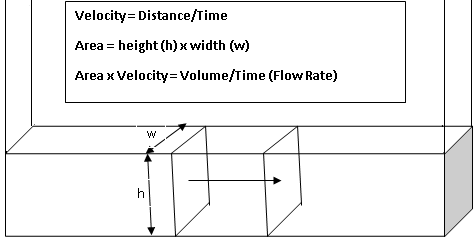
\includegraphics[scale=0.5]{ChannelFlow3}\\
$Q=V*A \implies Q = 1.5 \dfrac{ft}{sec}*(3*2)ft^2=\boxed{9\dfrac{ft^3}{sec}}$

Solution:\\
\vspace{0.5cm}
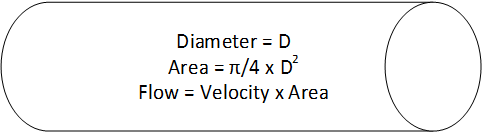
\includegraphics[scale=0.5]{PipeFlow}\\
$Q=V*A$\\
$\implies V=\dfrac{Q}{A} \implies V \Big(\dfrac{ft}{s}\Big)= \dfrac{\dfrac{500\cancel{gallon}}{\cancel{min}}*\dfrac{\cancelto{ft}{ft^3}*\dfrac{min}{60sec}}{7.48\cancel{gal}}}{0.785*\Big(\dfrac{8}{12}\Big)^2\cancelto{}{ft^2}}=\boxed{3.2ft/s}$

Solution:\\

\vspace{0.5cm}

The diameter of the pipe is 4 inches. Therefore, the radius is 2 inches. Convert the 2 inches to feet.
$
\begin{aligned}
&\dfrac{2}{12}=0.6667 \mathrm{ft} \\
&\mathrm{A}=\pi \times \mathrm{r}^{2} \\
&\mathrm{~A}=\pi \times(0.167 \mathrm{ft})^{2} \\
&\mathrm{~A}=\pi \times 0.028 \mathrm{ft}^{2} \\
&\mathrm{~A}=0.09 \mathrm{ft}^{2} \\
&\mathrm{Q}=\mathrm{V} \times \mathrm{A} \\
&\mathrm{Q}=1.5 \mathrm{ft} / \mathrm{sec} \times 0.09 \mathrm{ft}^{2} \\
&\mathrm{Q}=0.14 \mathrm{ft} / 3 \mathrm{sec}(\mathrm{cfs})
\end{aligned}
$



\vspace{1cm}

\vspace{1cm}

\section*{Practice Problems - Unit Conversions}
Convert the following:\\

Convert 1000 $ft^3$ to cu. yards\\

Convert 10 gallons/min to $ft^3$/hr\\

Convert 100,000 $ft^3$ to acre-ft.\\

Find the flow in gpm when the total flow for the day is 65,000 gpd.

Find the flow in gpm when the flow is $1.3 \mathrm{cfs}$.

Find the flow in gpm when the flow is $0.25 \mathrm{cfs}$.

The flow rate through a filter is 4.25 MGD. What is this flow rate expressed as gpm?\\

After calibrating a chemical feed pump, you've determined that the maximum feed rate is $178 \mathrm{~mL} /$ minute. If this pump ran continuously, how many gallons will it pump in a full day?

A plant produces 2,000 cubic foot of water per hour. How many gallons of water is produced in an 8-hour shift?

Change 70 °F to °C
Change 140 °F to °C
Change 20 °C to °F
Change 85 °C to °F
Change 4 °C to °F

\textbf{Solution}

Solution:\\

$1000 \cancel{ft^3}*\dfrac{cu.yards}{27\cancel{ft^3}} = 37 cu.yards$

Solution:\\

\vspace{0.4cm}

$\dfrac{10 \enspace \cancel{\mathrm{gallons}}}{\cancel{\mathrm{min}}}*  \dfrac{\mathrm{ft}^3}{7.48 \cancel{\mathrm{gallons}}}  * \dfrac{60 \cancel{\mathrm{min}}}{\mathrm{hr}}   = \dfrac{80.2 \enspace \mathrm{ft}^3}{\mathrm{hr}}$

\vspace{0.4cm}


Solution:\\

\vspace{0.4cm}

$100,000 \cancel{ft^3} * \dfrac{acre-ft}{43,560 \cancel{ft^2-ft}} =  2.3 acre-ft$\\

\vspace{0.2cm}

\textbf{Note:} From the conversion table: acre = 43,560 $ft^2$\\
Thus, acre-ft  = 43,560 $ft^2$-ft or 43,560 $ft^3$\\

\vspace{0.4cm}

Solution:\\

\vspace{0.4cm}

$
\dfrac{65,000 \mathrm{gpd}}{1,440 \mathrm{~min} / \mathrm{day}}=45 \mathrm{gpm}
$

\vspace{0.4cm}

Solution:\\
$
1.3 \dfrac{\mathrm{cfs}}{1} \mathrm{x} \dfrac{448 \mathrm{gpm}}{1 \mathrm{cfs}}=582 \mathrm{gpm}
$

\vspace{0.4cm}

Solution:\\

\vspace{0.4cm}

$
0.25 \dfrac{\mathrm{cfs}}{1} \times \dfrac{448 \mathrm{gpm}}{1 \mathrm{cfs}}=112 \mathrm{gpm}
$

\vspace{0.4cm}

Solution:\\

\vspace{0.2cm}

$Flow rate, gpm=\dfrac{Flow \enspace rate, \enspace gpd}{1440 \enspace min/day}$\\

\vspace{0.2cm}

Note:  We are assuming that the filter operated uniformly over that 24 hour period.\\

\vspace{0.3cm}

$Flow rate, gpm=\dfrac{4.25 \enspace \dfrac{\cancel{MG}}{\cancel{day}} *1,000,000 \enspace \dfrac{gal}{\cancel{MG}}}{1440\dfrac{min}{\cancel{day}}}=\boxed{2,951 \enspace gpm}$


Solution:\\

\vspace{0.4cm}

$\dfrac{2000 \enspace \cancel{\mathrm{ft}^3}}{\cancel{hr}}*  \dfrac{7.48 \enspace{\mathrm{gallons}}}{\cancel{\mathrm{ft}^3}}  * \dfrac{60 \enspace \cancel{\mathrm{hr}}}{\mathrm{shift}}   = \boxed{\dfrac{119,680 \enspace \mathrm{gallons}}{\mathrm{shift}}}$

\vspace{0.4cm}



\vspace{1cm}

\section*{Practice Problems - Concentration}

What is the concentration in mg/l of  4.5\% solution of that substance.

How many lbs of salt is needed to make 5 gallons of a 2,500mg/l solution


\vspace{0.5cm}
\textbf{Solution}\\

45,000 mg/l

Applying pounds formula:  lbs salt = $\dfrac{5}{1,000,000}*2,500*8.34=\boxed{0.14lbs}$



\vspace{1cm}
\section*{Practice Problems - Density and Specific Gravity}


What is the specific gravity of a 1 ft$^3$ concrete block which weighs 145 lbs?

What is the specific gravity of a chlorine solution if 1 (one) gallon weighs 10.2lbs?

How much does each gallon of zinc orthophosphate weigh (pounds) if it has a specific gravity of 1.46?

How much does a 55 gallon drum of 25\% caustic soda weigh (pounds) if the specific gravity is 1.28?



\section*{Practice Problems - Detention Time}

A flocculation basin is 7 ft deep, 15 ft wide, and 30 ft long. If the flow through the basin is 1.35 MGD, what is the detention time in minutes?

A tank has a diameter of 60 feet with an overflow depth at 44 feet. The current water level is 16 feet. Water is flowing into the tank at a rate of 250 gallons per minute. At this rate, how many days will it take to fill the tank to the overflow?

How long will it take to fill a 50 gallon hypochlorite tank if the flow is $5 \mathrm{gpm}$ ?

Find the detention time in a 45,000 gallon reservoir if the flow rate is $85 \mathrm{gpm}$.

If the fuel consumption to the boiler is 35 gallons per day. How many days will the 500 gallon tank last.

The sedimentation basin on a water plant contains 5,775 gallons. What is the detention time if the flow is $175 \mathrm{gpm}$.


\textbf{Solution}\\

Solution:\\
\vspace{0.5cm}
\begin{tikzpicture}

\pgfmathsetmacro{\cubexx}{4}
\pgfmathsetmacro{\cubeyy}{1.5}
\pgfmathsetmacro{\cubezz}{2}
\pgfmathsetmacro{\cubex}{4}
\pgfmathsetmacro{\cubey}{0.5}
\pgfmathsetmacro{\cubez}{2}
\filldraw [fill=lightgray!20, draw=black] (0,-\cubey,0) -- ++(-\cubexx,0,0) -- ++(0,-\cubeyy,0) -- ++(\cubexx,0,0) -- cycle ;
\filldraw [fill=lightgray!20, draw=black] (0,-\cubey,0) -- ++(0,0,-\cubezz) -- ++(0,-\cubeyy,0) -- ++(0,0,\cubezz) -- cycle;
\filldraw [fill=lightgray!20, draw=black] (0,-\cubey,0) -- ++(0,0,-\cubezz) -- ++(0,-\cubeyy,0) -- ++(0,0,\cubezz) -- cycle;
\filldraw [fill=lightgray!20, draw=black] (0,-\cubey,0) -- ++(-\cubexx,0,0) -- ++(0,0,-\cubezz) -- ++(\cubexx,0,0) -- cycle;
%\draw (0,-0.5,0) -- ++(-\cubex,0,0) -- ++(0,-\cubey,-\cubez) -- ++(\cubex,0,0) -- cycle;
\draw (-\cubex,0,0) -- ++(0,0,-\cubez) -- ++(0,-\cubey,0) -- ++(0,0,\cubez) -- cycle;
\draw (0,-\cubey,0) -- ++(-\cubex,0,0) -- ++(0,0,-\cubez) -- ++(\cubex,0,0) -- cycle;




\filldraw [fill=white, draw=black] (0,0,0) -- ++(-\cubex,0,0) -- ++(0,-\cubey,0) -- ++(\cubex,0,0) -- cycle ;
\filldraw [fill=white, draw=black] (0,0,0) -- ++(0,0,-\cubez) -- ++(0,-\cubey,0) -- ++(0,0,\cubez) -- cycle;
\filldraw [fill=white, draw=black] (0,0,0) -- ++(0,0,-\cubez) -- ++(0,-\cubey,0) -- ++(0,0,\cubez) -- cycle;
\filldraw [fill=white, draw=black] (0,0,0) -- ++(-\cubex,0,0) -- ++(0,0,-\cubez) -- ++(\cubex,0,0) -- cycle;
%\draw (0,-0.5,0) -- ++(-\cubex,0,0) -- ++(0,0,-\cubez) -- ++(\cubex,0,0) -- cycle;
%\filldraw [fill=white, draw=black] (-\cubex,0,0) -- ++(0,0,-\cubez) -- ++(0,-\cubey,0) -- ++(0,0,\cubez) -- cycle;
%\filldraw [fill=white, draw=black] (0,-\cubey,0) -- ++(-\cubex,0,0) -- ++(0,0,-\cubez) -- ++(\cubex,0,0) -- cycle;

\draw [<->] (-4,-2.3) -- (0,-2.3) node [midway, below] {\scriptsize{30' long}};
\draw [<->] (1,-1.3) -- (1,.2) node [midway, below] {\hspace{2.2cm}\scriptsize{7' deep}};
%\draw [<->] (1,.8) -- (1,.2) node [midway, below] {\hspace{2.2cm}Text Y Axis};
\draw [<->] (1,-1.3) -- (0,-2.3) node [midway, below] {\hspace{1.7cm}\scriptsize{15' wide}};
\draw [->](-6,-1) -- (-4,-1) node [midway, above] {\hspace{0.5cm}\scriptsize{1.5 MGD}};
\draw [->](0.3,-1) -- (0.9,-1) node [midway, above] {};
\end{tikzpicture}\\

\vspace{0.4cm}
$
\mathrm{DT}=\dfrac{(30*15*7) \mathrm{ft^3}*7.48\dfrac{gal}{ft^3}}{1,350,000 \dfrac{\mathrm{gal}}{day}*\dfrac{\mathrm{day}}{1440\mathrm{min}}}=25 \mathrm{min}
$


\vspace{0.4cm}


Solution:\\

\vspace{0.4cm}
\begin{tikzpicture}[scale=1]
\node [draw, cylinder, cylinder uses custom fill, cylinder body fill=green!20, 
cylinder end fill=green!20, shape aspect=4, rotate=90, minimum width=3cm] (c1) at 
(0,1.8){};

\coordinate(dhtop) at ($(c1.after top)!-1*.1!(c1.before top)$);
\coordinate(dhbot) at ($(c1.before bottom)!-1*.1!(c1.after bottom)$);
\coordinate(dhlabel) at ($(dhtop)!.5!(dhbot)$);
%\draw[|-|] (dhbot)--(dhtop);
%\path (dhlabel) node[right, outer sep = 2pt] {$44'$};

\node [draw, cylinder, cylinder body fill=black!20, cylinder end fill=red!20, shape aspect=4, rotate=90, minimum height=4cm, minimum width=3cm] (c) {};

\coordinate(htop) at ($(c.before top)!-1*.1!(c.after top)$);
\coordinate(hbot) at ($(c.after bottom)!-1*.1!(c.before bottom)$);
\coordinate(hlabel) at ($(htop)!.5!(hbot)+(c.north)!.9!(c.center)$);

%\draw[|-|] (hbot)--(htop);
%\path (hlabel) node[left] {}; %Modify height label here


%\node [draw, cylinder, cylinder uses custom fill, cylinder body fill=black!20, 
%cylinder end fill=lightgray!20, shape aspect=4, rotate=90, minimum width=3cm] (c1) at 
%(0,3.8){};


\node [draw, cylinder, cylinder uses custom fill, cylinder body fill=black!20, 
cylinder end fill=lightgray!20, shape aspect=4, rotate=90, minimum width=3cm] (c1) at 
(0,-1.2){};

%\node [draw, cylinder, cylinder uses custom fill, cylinder body fill=blue!20, 
cylinder end fill=green!20, shape aspect=4, rotate=90, minimum width=3cm] (c1) at 
(0,0){};

%\coordinate (center) at ($(c.before top)!0.5!(c.after top)$);
%\filldraw (center) circle (1pt);
%
%\coordinate (rlabel) at ($(center) !0.5!(c.after top)$);
%\coordinate (rtop) at ($(center)!-1*.1!(c.after top)$);

%\coordinate (rend) at ($(c.mid east)!0.5!(c.after top)$);
%\draw[-, shorten >=-10] (center) -- (rend);
%\path (rend) node[outer sep = 5pt, left] {$r$};
\draw [<->] (-1.5,2.4) -- (1.5,2.4) node [midway, above=1mm] {\hspace{0.05cm}\scriptsize{Diameter=60'}};
%\draw [<->] (1.8,2.4) -- (1.8,1.9) node [midway, midway] {\hspace{2.4cm}\scriptsize{16' Freeboard}};
%\draw [<->] (1.8,1.9) -- (1.8,-0.7) node [midway, midway] {\hspace{2.4cm}\scriptsize{28' Fill}};
%\draw [<->] (1.8,-1.1) -- (1.8,-0.7) node [midway, midway] {\hspace{2.8cm}\scriptsize{16' Current Level}};
\draw (3.3,1.9) node{\scriptsize{Overflow level = 44'}};
\draw (3.22,-0.6) node{\scriptsize{Current level = 16'}};
\draw [<-] (1.5,-0.6) -- (2.2,-0.6);
\draw [<-] (1.5,1.9) -- (2.2,1.9);
\draw[thick,->](0,3.5)--(0,2.5) node [at start, above, black] (n){\scriptsize{250 gpm}};
\end{tikzpicture}

$\mathrm{Fill \enspace time}=\dfrac{Volume}{Flow}=\dfrac{0.785*60^2*(44-16)ft^3*\dfrac{7.48 gallons}{ft^3}}{250 \dfrac{gallons}{min}*\dfrac{1440 \enspace min}{day}}=1.6 \enspace days$
\vspace{0.4cm}

Solution:\\4

\vspace{0.4cm}



\vspace{0.4cm}

Solution:\\5

\vspace{0.4cm}

$
\mathrm{DT}=\dfrac{50 \mathrm{gal}}{5 \mathrm{gal} / \mathrm{min}}=10 \mathrm{~min}
$

\vspace{0.4cm}

Solution:\\

\vspace{0.4cm}

$
\mathrm{DT}=\dfrac{45,000 \mathrm{gal}}{85 \mathrm{gal} / \mathrm{min}}=529 \mathrm{~min} \quad \text { or } \dfrac{529 \mathrm{~min}}{60 \mathrm{~min} / \mathrm{hr}}=8.8 \mathrm{hrs}
$
\vspace{0.4cm}

Solution:\\

\vspace{0.4cm}

$
\mathrm{DT}=\dfrac{500 \text { gal }}{35 \mathrm{gal} / \text { day }}=14.3 \text { days }
$
\vspace{0.4cm}

Solution:\\

\vspace{0.4cm}

$
\mathrm{DT}=\dfrac{5,775 \mathrm{gal}}{175 \mathrm{gal} / \mathrm{min}}=33 \mathrm{~min}
$


\vspace{1cm}

\section*{Practice Problems - Unit Conversions}

Convert 22\degree{C} into degree Fahrenheit.
Convert 56\degree{C} into degree Celsius.

\vspace{1cm}

\section*{Practice Problems - Pounds Formula}


A water treatment plant operates at the rate of 75 gallons per minute. They dose soda ash at
14 mg/L. How many pounds of soda ash will they use in a day?

A water treatment plant is producing 1.5 million gallons per day of potable water, and
uses 38 pounds of soda ash for pH adjustment. What is the dose of soda ash at that plant?

A water treatment plant produces 150,000 gallons of water every day. It uses an
average of 2 pounds of permanganate for iron and manganese removal. What is the dose of the
permanganate? 

A water treatment plant uses 8 pounds of chlorine daily and the dose is 17 mg/l. How
many gallons are they producing?

An operator mixes 40 lb of lime in a 100-gal tank containing 80 gal of water. What is the percent of lime in the slurry?

A treatment plant has a maximum output of $30 \mathrm{MGD}$ and doses ferric chloride at 75 $\mathrm{mg} / \mathrm{L}$. How many pounds of Ferric Chloride does the plant use in a day?\\

 A treatment plant uses 750 pounds of alum a day as it treats $15 \mathrm{MGD}$. What was the dose rate?\\


 A treatment plant operates at 1,500 gallons a minute and uses 500 pounds of alum a day. What is the alum dose?\\



\textbf{Solution:}
[1.]
Solution:\\

\begin{figure}[h]
\begin{tikzpicture}
    \newcommand{\R}{1.5}

\path[help lines,step=.2] (0,0) grid (16,3);
\path[help lines,line width=.6pt,step=1] (0,0) grid (16,3);
%\foreach \x in {0,1,2,3,4,5,6,7,8,9,10,11,12,13,14,15,16}
%\node[anchor=north] at (\x,0) {\x};
%\foreach \y in {0,1,2,3,4,5,6}
%\node[anchor=east] at (0,\y) {\y};
%-------------CIRCLE-----------------------------------
\draw[black,fill=gray!10] (8,3) circle (\R);
\draw[black, very thick, rotate=0](6.5,3) -- (9.5,3);
\draw (8,3.6) node[text width=3cm,align=center]
  {\scriptsize{lbs/day}};
\draw (7.1,2.5) node[text width=3cm,align=center]
  {\tiny{14 mg/l}};
\draw (8.9,2.5) node[text width=3cm,align=center]
  {\tiny{75 GPM}};
  \draw (8,2)node[text width=3cm,align=center]
  {\tiny{8.34}};
\draw[black, very thick, rotate=0](7.2,1.7) -- (8,3);
\draw[black, very thick, rotate=0](8.8,1.7) -- (8,3);
\end{tikzpicture}
\end{figure}
$\dfrac{\mathrm{lbs}}{\mathrm{day}}=\mathrm{Flow}\dfrac{{\mathrm{MG}}}{\mathrm{day}}* \mathrm{Concentration}\dfrac{\mathrm{mg}}{\mathrm{l}}*8.34$
\\
\vspace{0.2cm}
$\dfrac{\mathrm{lbs}}{\mathrm{day}}=75 \dfrac{\cancel{\mathrm{gallons}}}{\cancel{\mathrm{min}}}* 1440\dfrac{\cancel{\mathrm{min}}}{\mathrm{day}}*\dfrac{\mathrm{MG}}{1,000,000 \enspace \cancel{\mathrm{gallons}}}*250\dfrac{\mathrm{mg}}{\mathrm{l}}*8.34 = \boxed{225\dfrac{lbs}{day}}$
\vspace{0.2cm}
 Solution:\\
 \begin{figure}[h!]
\begin{tikzpicture}
    \newcommand{\R}{1.5}

\path[help lines,step=.2] (0,0) grid (16,3);
\path[help lines,line width=.6pt,step=1] (0,0) grid (16,3);
%\foreach \x in {0,1,2,3,4,5,6,7,8,9,10,11,12,13,14,15,16}
%\node[anchor=north] at (\x,0) {\x};
%\foreach \y in {0,1,2,3,4,5,6}
%\node[anchor=east] at (0,\y) {\y};
%-------------CIRCLE-----------------------------------
\draw[black,fill=gray!10] (8,3) circle (\R);
\draw[black, very thick, rotate=0](6.5,3) -- (9.5,3);
\draw (8,3.6) node[text width=3cm,align=center]
  {\scriptsize{38 lbs/day}};
\draw (7.1,2.5) node[text width=3cm,align=center]
  {\tiny{? mg/l}};
\draw (8.9,2.5) node[text width=3cm,align=center]
  {\tiny{1.5 MGD}};
  \draw (8,2)node[text width=3cm,align=center]
  {\tiny{8.34}};
\draw[black, very thick, rotate=0](7.2,1.7) -- (8,3);
\draw[black, very thick, rotate=0](8.8,1.7) -- (8,3);
\end{tikzpicture}
\end{figure}
$\dfrac{\mathrm{lbs}}{\mathrm{day}}=\mathrm{Flow}\dfrac{{\mathrm{MG}}}{\mathrm{day}}* \mathrm{Concentration}\dfrac{\mathrm{mg}}{\mathrm{l}}*8.34 \hspace{0.2cm} \implies \mathrm{Concentration}\dfrac{\mathrm{mg}}{\mathrm{l}}=\dfrac{ \dfrac{\mathrm{lbs}}{\mathrm{day}}}{\mathrm{Flow}\dfrac{{\mathrm{MG}}}{\mathrm{day}}*8.34}$
\vspace{0.2cm}
$\mathrm{Concentration}\dfrac{\mathrm{mg}}{\mathrm{l}}=\dfrac{ 38\dfrac{\mathrm{lbs}}{\mathrm{day}}}{1.5\dfrac{{\mathrm{MG}}}{\mathrm{day}}*8.34}=\boxed{3\dfrac{\mathrm{mg}}{\mathrm{l}}}$
\\
\vspace{0.2cm}



 Solution:\\
 \begin{figure}[h!]
\begin{tikzpicture}
    \newcommand{\R}{1.5}

\path[help lines,step=.2] (0,0) grid (16,3);
\path[help lines,line width=.6pt,step=1] (0,0) grid (16,3);
%\foreach \x in {0,1,2,3,4,5,6,7,8,9,10,11,12,13,14,15,16}
%\node[anchor=north] at (\x,0) {\x};
%\foreach \y in {0,1,2,3,4,5,6}
%\node[anchor=east] at (0,\y) {\y};
%-------------CIRCLE-----------------------------------
\draw[black,fill=gray!10] (8,3) circle (\R);
\draw[black, very thick, rotate=0](6.5,3) -- (9.5,3);
\draw (8,3.6) node[text width=3cm,align=center]
  {\scriptsize{38 lbs/day}};
\draw (7.1,2.5) node[text width=3cm,align=center]
  {\tiny{? mg/l}};
\draw (8.9,2.5) node[text width=3cm,align=center]
  {\tiny{1.5 MGD}};
  \draw (8,2)node[text width=3cm,align=center]
  {\tiny{8.34}};
\draw[black, very thick, rotate=0](7.2,1.7) -- (8,3);
\draw[black, very thick, rotate=0](8.8,1.7) -- (8,3);
\end{tikzpicture}
\end{figure}
$\dfrac{\mathrm{lbs}}{\mathrm{day}}=\mathrm{Flow}\dfrac{{\mathrm{MG}}}{\mathrm{day}}* \mathrm{Concentration}\dfrac{\mathrm{mg}}{\mathrm{l}}*8.34 \hspace{0.2cm} \implies \mathrm{Concentration}\dfrac{\mathrm{mg}}{\mathrm{l}}=\dfrac{ \dfrac{\mathrm{lbs}}{\mathrm{day}}}{\mathrm{Flow}\dfrac{{\mathrm{MG}}}{\mathrm{day}}*8.34}$
\vspace{0.2cm}
$\mathrm{Concentration}\dfrac{\mathrm{mg}}{\mathrm{l}}=
\dfrac{ 2\dfrac{\mathrm{lbs}}{\mathrm{day}}}
{\Bigg(150,000 \dfrac{\cancel{\mathrm{Gallons}}}
{\mathrm{day}}*
\dfrac{\mathrm{MG}}
{1,000,000 \cancel{\enspace \mathrm{Gallons}}}*8.34\Bigg)}
=\boxed{3\dfrac{\mathrm{mg}}{\mathrm{l}}}$
\\
\vspace{0.2cm}


 Solution:\\
 \begin{figure}[h!]
\begin{tikzpicture}
    \newcommand{\R}{1.5}

\path[help lines,step=.2] (0,0) grid (16,3);
\path[help lines,line width=.6pt,step=1] (0,0) grid (16,3);
%\foreach \x in {0,1,2,3,4,5,6,7,8,9,10,11,12,13,14,15,16}
%\node[anchor=north] at (\x,0) {\x};
%\foreach \y in {0,1,2,3,4,5,6}
%\node[anchor=east] at (0,\y) {\y};
%-------------CIRCLE-----------------------------------
\draw[black,fill=gray!10] (8,3) circle (\R);
\draw[black, very thick, rotate=0](6.5,3) -- (9.5,3);
\draw (8,3.6) node[text width=3cm,align=center]
  {\scriptsize{8 lbs/day}};
\draw (7.1,2.5) node[text width=3cm,align=center]
  {\tiny{17 mg/l}};
\draw (8.9,2.5) node[text width=3cm,align=center]
  {\tiny{? MGD}};
  \draw (8,2)node[text width=3cm,align=center]
  {\tiny{8.34}};
\draw[black, very thick, rotate=0](7.2,1.7) -- (8,3);
\draw[black, very thick, rotate=0](8.8,1.7) -- (8,3);
\end{tikzpicture}
\end{figure}
$\dfrac{\mathrm{lbs}}{\mathrm{day}}=\mathrm{Flow}\dfrac{{\mathrm{MG}}}{\mathrm{day}}* \mathrm{Concentration}\dfrac{\mathrm{mg}}{\mathrm{l}}*8.34 \hspace{0.2cm}$\\
\vspace{0.2cm}
$\implies \mathrm{Flow}\dfrac{{\mathrm{MG}}}{day}=\dfrac{ \dfrac{\mathrm{lbs}}{\mathrm{day}}}{\mathrm{Concentration}\dfrac{\mathrm{mg}}{\mathrm{l}}*8.34}=\dfrac{8 \dfrac{\mathrm{lbs}}{\mathrm{day}}}{17\dfrac{\mathrm{mg}}{\mathrm{l}}*8.34}=0.056425\dfrac{{\mathrm{MG}}}{day}$\\
\vspace{0.2cm}
$0.056425\dfrac{{\mathrm{MG}}}{day}*\dfrac{1,000,000 \enspace \mathrm{Gallons}}{\mathrm{MG}}=\boxed{56,425 \enspace \mathrm{Gallons}}$
\vspace{0.2cm}


 Solution:\\
 \begin{figure}[h!]
\begin{tikzpicture}
    \newcommand{\R}{1.5}

\path[help lines,step=.2] (0,0) grid (16,3);
\path[help lines,line width=.6pt,step=1] (0,0) grid (16,3);
%\foreach \x in {0,1,2,3,4,5,6,7,8,9,10,11,12,13,14,15,16}
%\node[anchor=north] at (\x,0) {\x};
%\foreach \y in {0,1,2,3,4,5,6}
%\node[anchor=east] at (0,\y) {\y};
%-------------CIRCLE-----------------------------------
\draw[black,fill=gray!10] (8,3) circle (\R);
\draw[black, very thick, rotate=0](6.5,3) -- (9.5,3);
\draw (8,3.6) node[text width=3cm,align=center]
  {\scriptsize{38 lbs/day}};
\draw (7.1,2.5) node[text width=3cm,align=center]
  {\tiny{? mg/l}};
\draw (8.9,2.5) node[text width=3cm,align=center]
  {\tiny{1.5 MGD}};
  \draw (8,2)node[text width=3cm,align=center]
  {\tiny{8.34}};
\draw[black, very thick, rotate=0](7.2,1.7) -- (8,3);
\draw[black, very thick, rotate=0](8.8,1.7) -- (8,3);
\end{tikzpicture}
\end{figure}
$\mathrm{lbs}=\mathrm{Volume}{\mathrm{(MG)}}* \mathrm{Concentration}\dfrac{\mathrm{mg}}{\mathrm{l}}*8.34 \hspace{0.2cm}$\\
\vspace{0.2cm}
$ \implies \mathrm{Concentration}\dfrac{\mathrm{mg}}{\mathrm{l}}=\dfrac{ \mathrm{lbs}}{\mathrm{Volume}\mathrm{(MG)}*8.34}=\dfrac{40 \enspace \mathrm{lbs}}{80 \enspace\mathrm{gallons}*\dfrac{\mathrm{MG}}{1,000,000 \enspace \cancel{\mathrm{gallons}}}*8.34}$
\vspace{0.2cm}

\vspace{0.2cm}




%\mathrm{Concentration}\dfrac{\mathrm{mg}}{\mathrm{l}}
\vspace{1cm}







\section*{Practice Problems - Pressure-Force Relationship}

  Find the force on a 12-inch valve if the water pressure within the line is 60 psi. Express your answer in tons.

$\textrm{Force}= \textrm{Pressure} \times \textrm{Area}$\\
\vspace{0.3cm}
$\implies 60 \enspace \dfrac{\mathrm{lbs}}{\mathrm{in^2}}*0.785 *(12 \mathrm{in})^2*\dfrac{1 \mathrm{ton}}{2000 \mathrm{lbs}} =\boxed{3.39 \enspace\mathrm{tons}}$
\vspace{0.3cm}
  A 42-inch main line has a shut off valve. The same line has a 10-inch bypass line with another shut-off valve. Find the amount of force on each valve if the water pressure in the line is 80 psi. Express your answer in tons.\\

\vspace{0.5cm}
$\textrm{Force}= \textrm{Pressure} \times \textrm{Area}$\\
\vspace{0.5cm}

\vspace{0.5cm}
Calculating the force from the 42" line on the shutoff valve:\\

\vspace{0.3cm}
$\implies 80 \enspace \dfrac{\mathrm{lbs}}{\mathrm{in^2}}*0.785 *(42 \mathrm{in})^2*\dfrac{1 \mathrm{ton}}{2000 \mathrm{lbs}} =\boxed{55 \enspace\mathrm{tons}}$\\

\vspace{0.3cm}
Calculating the force from the 10" line on the shutoff valve:\\

\vspace{0.3cm}
$\implies 80 \enspace \dfrac{\mathrm{lbs}}{\mathrm{in^2}}*0.785 *(10 \mathrm{in})^2*\dfrac{1 \mathrm{ton}}{2000 \mathrm{lbs}} =\boxed{3.14 \enspace\mathrm{tons}}$\\

  A water tank is 15 feet deep and 30 feet in diameter. What is the force exerted on a 6-inch valve at the bottom of the tank?\\
\vspace{0.5cm}
$\textrm{Force}= \textrm{Pressure} \times \textrm{Area}$\\
\vspace{0.5cm}
$\implies 15 \enspace\mathrm{ft}* \dfrac{0.433 \enspace \mathrm{psi}}{\mathrm{ft}}*0.785 *(6 \mathrm{in})^2 =\boxed{183 \enspace\mathrm{lbs}}$\\
\vspace{0.3cm}

\vspace{1cm}

\section*{Practice Problems - Well Hydraulics}


A well yields 2,840 gallons in exactly 20 minutes. What is the well yield in gpm?\\
a. 140 gpm\\
b. 142 gpm\\
c. 145 gpm\\
d. 150 gpm

A well is producing $1.25 \mathrm{MGD}$. Its static water level was $35 \mathrm{ft}$ bgs, and its current pumping water level is $115 \mathrm{ft}$ bgs. What is the specific capacity of this well?\\
a. $\quad 0.016 \mathrm{gpm} / \mathrm{ft}$\\
b. $\quad 4.7 \mathrm{gpm} / \mathrm{ft}$\\
c. $\quad 10.9 \mathrm{gpm} / \mathrm{ft}$\\
d. $\quad 15.6 \mathrm{gpm} / \mathrm{ft}$\\
e. $\quad 100 \mathrm{gpm} / \mathrm{ft}$\\

Before pumping, the water level in a well is 15 ft. down. During pumping, the water level is 45 ft. down. The draw-down is:\\
a. 30 ft.\\
b. 60 ft.\\
c. 45 ft.\\
d. 15 ft.\\

A well produces 365 gpm with a drawdown of 22.5 ft.  What is	the specific yield in gallons per minute per foot?\\
a.	16.2\\
b.	22.5\\
c.	32.4\\
d.	86.5\\

.	A well is located in an aquifer with a water table elevation 20 feet below the ground surface. After operating for three hQ!Jrs, the water level in the well stabilizes at 50 feet below the ground surface. The pumping water level is:\\
a.	20 feet\\
b.  30 feet\\
c.	50 feet\\
d.	70 feet\\
e.	100 feet\\

Calculate drawdown, in feet, using the following data:\\
The water level in a well is 20 feet below the ground surface when the pump is not in operation, and the water level is 35 feet below the ground surface when the pump is in operation.\\
a.	15 feet\\
b.	20 feet\\
c.	35 feet\\
d.	55 feet\\

Calculate the well yield in gpm, given a drawdown of 14.1 ft and a specific yield of 31
gpm/ft.\\
a. 2.2 gpm\\
b. 7.3 gpm\\
c. 45.1 gpm \\
d. 440 gpm\\

A well is producing 1.25 MGD. Its static water level was 35 ft and its current pumping
water level is 115 ft. What is the specific capacity of this well? \\
a. 0.016 gpm/ft\\
b. 4.7 gpm/ft\\
c. 10.9 gpm/ft\\
d. 15.6 gpm/ft\\
e. 100 gpm/ft\\

Determine the drawdown from a well measuring a static water level of 120 feet and a pumping water level of 205 feet?\\
a. 105 ft\\
b. 320 feet\\
c. 85 feet\\
d. 310 feet\\

Before pumping, the static water level in a well is 15 feet. During pumping, the water
level drops to 45 feet. What is the drawdown?\\
a. 15 ft\\
b. 30 ft\\
c. 45 ft\\
d. 60 ft\\
e. 90 ft\\

The specific capacity for a well is 10 gpm-ft. If the well produces 550 gallons per minute, what is the drawdown?

The distance between the ground surface to the water level in a well when the pump is not operating is 98 ft.  Distance from the ground surface to the water in the well when the pump is operating is 116 feet. Calculate the drawdown in the well under these conditions.

What is the specific capacity in gpm/feet a well that is pumping 495 gpm and has a
static level of 55 feet and a pumping level of 110 feet?

During a test for well yield, a well produced 760 gallons per minute. The drawdown for the test is 22 feet What is the specific capacity in gallons per min-ft/?

The pumped water level of a well is 400 feet below the surface. The well produces  250 gpm.  If the aquifer level 50 feet below the surface, what is the specific capacity for the well




\section*{Practice Problems - Pumping Head}

Convert 45 psi to feet of head

How long (in minutes) will it take to pump down 25 feet of water in a 110 ft diameter cylindrical tank when using a 1420 gpm pump\\

How long will it take (hrs) to fill a 2 ac-ft pond if the pumping rate is 400 GPM?

If the pressure at a water main is 50 psi, what would the static pressure (psi) be at a faucet on the top floor of a four story building? (Assuming 10 ft. per story)

A water tower has water pressure of 98 psi at its base. What would be. the pressure at a hydrant three blocks away if there is a 65-foot head loss in the pipe?\\





\textbf{Solution:}


 Solution:\\ 
 \vspace{0.2cm}
$
45 \enspace \cancel{psi}*\dfrac{ft \enspace head}{0.433\cancel{psi}}=\boxed{103.9 \text { feet }}
$
 
 \vspace{0.2cm}
 
  Solution:\\
  
  $Time \enspace to \enspace pump \enspace down= \dfrac{Volume}{Flow}=\dfrac{0.785*110^2*25 \enspace \cancel{ft^3}}{1420\dfrac{\cancel{gallon}}{min}*\dfrac{\cancel{ft^3}}{7.48\cancel{gallon}}}=\boxed{190 \enspace minutes}$
 
 \vspace{0.2cm}

 Solution:\\
 
 \vspace{0.2cm}
 
 $Time \enspace to \enspace fill \enspace(hours)= \dfrac{Volume}{Flow}=\dfrac{2 \enspace \cancel{ac-ft}*\dfrac{325,851 \enspace \cancel{gallons}}{\cancel{ac-ft}}}{400 \dfrac{\cancel{gallons}}{\cancel{min}}*\dfrac{60 \enspace\cancel{ min}}{hr}}=\boxed{27 \enspace hours}$
 

 Solution:\\ 
 \vspace{0.2cm}
$
50 psi - 4*10 \enspace \cancel{ft}*\dfrac{0.433\cancel{psi}{ft \enspace head}}=\boxed{32.7 \text { psi}}
$


 Solution:\\ 
 \vspace{0.2cm}
$
98 psi - 65 \enspace \cancel{ft}*\dfrac{0.433\cancel{psi}{ft \enspace head \enspace loss}}=\boxed{70 \text { psi}}
$





\section*{Practice Problems - Pumping Power Requirements}

  If a pump is operating at 2,200 gpm and 60 feet of head, what is the water
horsepower? If the pump efficiency is 71\%, what is the brake horsepower?

The water horsepower of a pump is $10 \mathrm{Hp}$ and the brake horsepower output of the motor is $15.4 \mathrm{Hp}$. What is the efficiency of the pump?

The water horsepower of a pump is $25 \mathrm{Hp}$ and the brake horsepower output of the motor is $48 \mathrm{Hp}$. What is the efficiency of the pump?

The efficiency of a well pump is determined to be $75 \%$. The efficiency of the motor is estimated at $94 \%$. What is the efficiency of the well?

If a motor is $85 \%$ efficient and the output of the motor is determined to be 10
$\mathrm{BHp}$, what is the electrical horsepower requirement of the motor?

The water horsepower of a well with a submersible pump has been calculated at 8.2 WHp. The Output of the electric motor is measured as $10.3 \mathrm{BHp}$. What is the efficiency of the pump?

  Water is being pumped from a reservoir to a storage tank on a hill. The elevation difference between water levels is 1200 feet. Find the pump size required to fill the tank at a rate of 120 gpm. Express your answer in horsepower.

  A $25 \mathrm{hp}$ pump is used to dewater a lake. If the pump runs for 8 hours a day for 7 days a week, how much will it cost to run the pump for one week? Assume energy costs $\$ 0.07$ per kilowatt hour.

  A pump station is used to lift water 50 feet above the pump station to a storage tank. The pump rate is $500 \mathrm{gpm}$. If the pump has an efficiency of $85 \%$ and the motor has an efficiency of $90 \%$, find each of the following: Water Horsepower, Brake Horsepower, Motor Horsepower, and Wire-to-Water Efficiency.


  Find the brake horsepower for a pump given the following information: Total Dynamic Head $=75$ feet, Pump Rate $=150$ gpm, Pump Efficiency $=90 \%$, Motor Efficiency $=85 \%$

  Water is being pumped from a reservoir to a storage tank on a hill. The elevation difference between water levels is 1200 feet. Find the pump size required to fill the tank at a rate of 120 gpm. Express your answer in horsepower.




\textbf{Solutions:}



 Solution:\\
\vspace{0.4cm}
water Hp = flow * head\\
$2,200GPM*60ft*\dfrac{Hp}{3,960 GPM-ft}=\boxed{Water \enspace Hp = 33.3Hp}$\\
\vspace{0.4cm}
pump Hp = brake Hp * pump efficiency\\
$brake \enspace Hp = \dfrac{33.3}{0.71}=\boxed{Brake \enspace Hp=47Hp}$
 \vspace{0.2cm}

 Solution:\\ 
 \vspace{0.2cm}
 \vspace{0.4cm}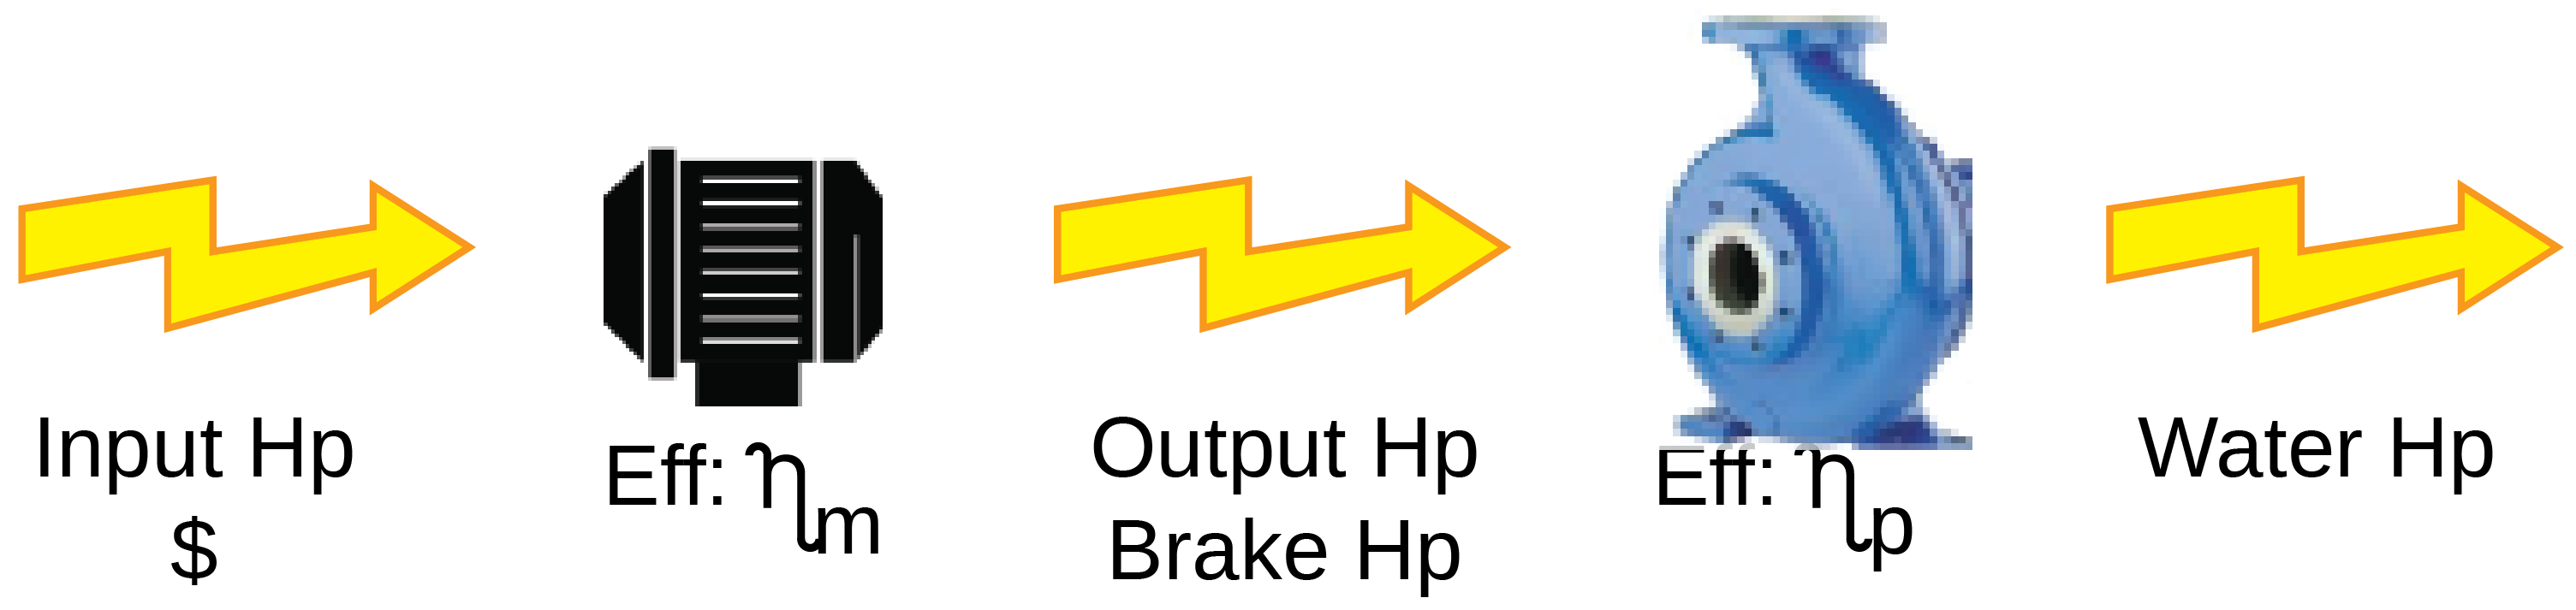
\includegraphics[scale=0.08]{PumpProblem}\\
 \vspace{0.2cm}
 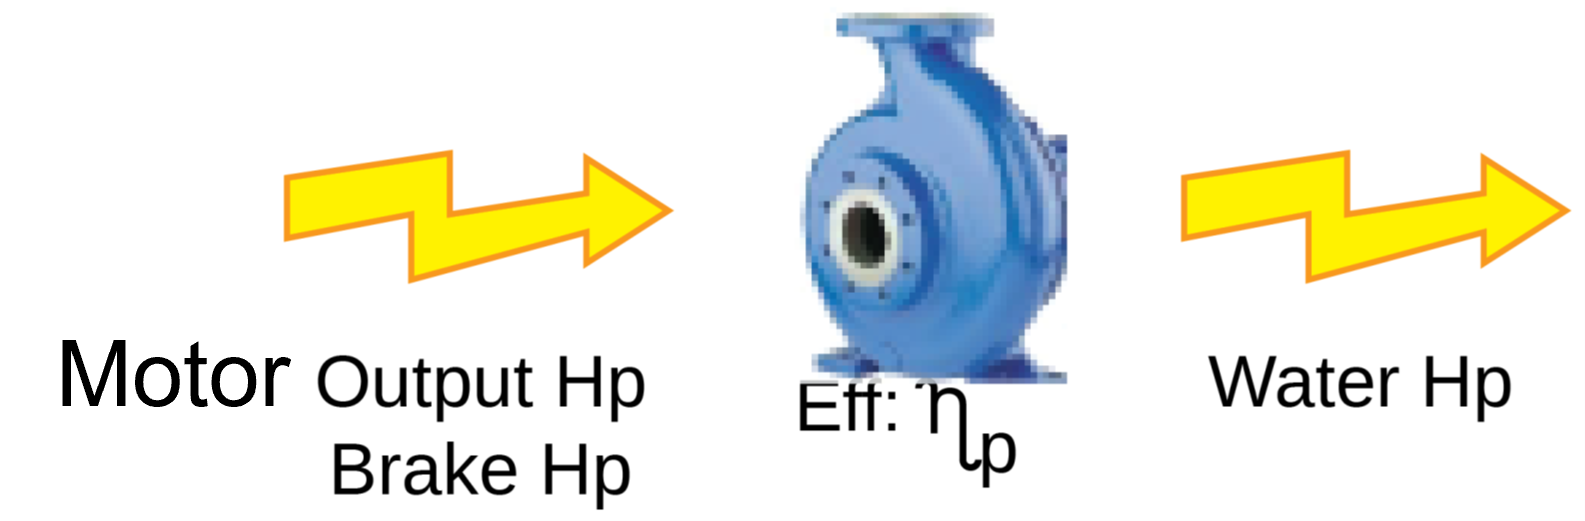
\includegraphics[scale=0.32]{PumpingProblemPump}
 $\eta_p=\dfrac{10 \mathrm{BHp}}{15.4 \mathrm{EHp}} \times 100=\boxed{65 \%}$
 \vspace{0.2cm}
 
 
 Solution:\\
  \vspace{0.2cm}
 \vspace{0.32cm}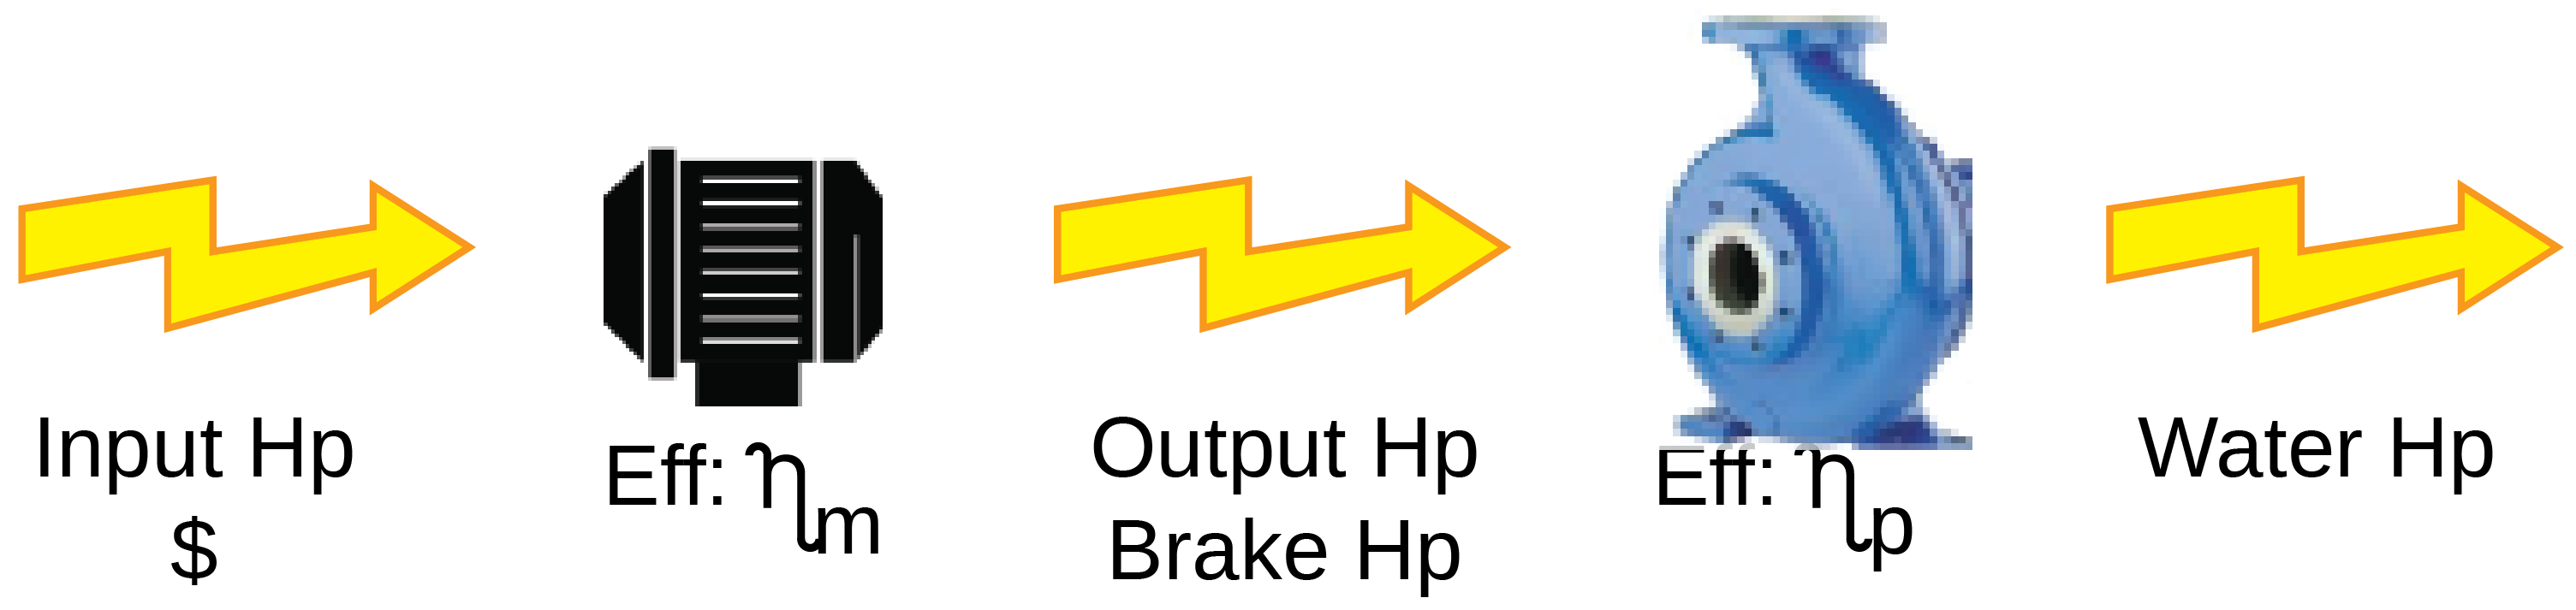
\includegraphics[scale=0.08]{PumpProblem}\\
 \vspace{0.2cm}
 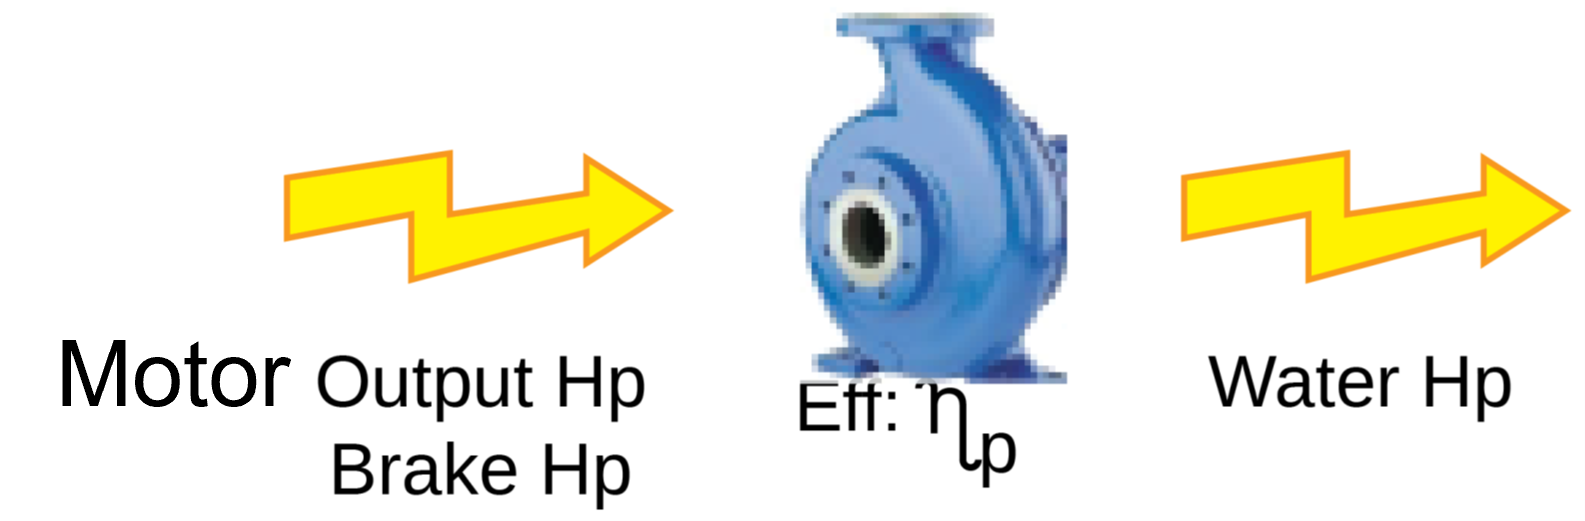
\includegraphics[scale=0.4]{PumpingProblemPump}
 \vspace{0.2cm}
$\eta_p=\dfrac{25 \mathrm{\enspace Water \enspace Hp}}{48 \mathrm{\enspace brake \enspace Hp}} \times 100=\boxed{52 \%}$
  \vspace{0.4cm}
 Solution:\\ 
 \vspace{0.2cm}
$Well \enspace efficiency=\eta_m * \eta_p \implies 0.94 \times 0.75=0.705 \times 100=\boxed{71 \%}$
 \vspace{0.2cm}


 Solution:\\
 \vspace{0.4cm}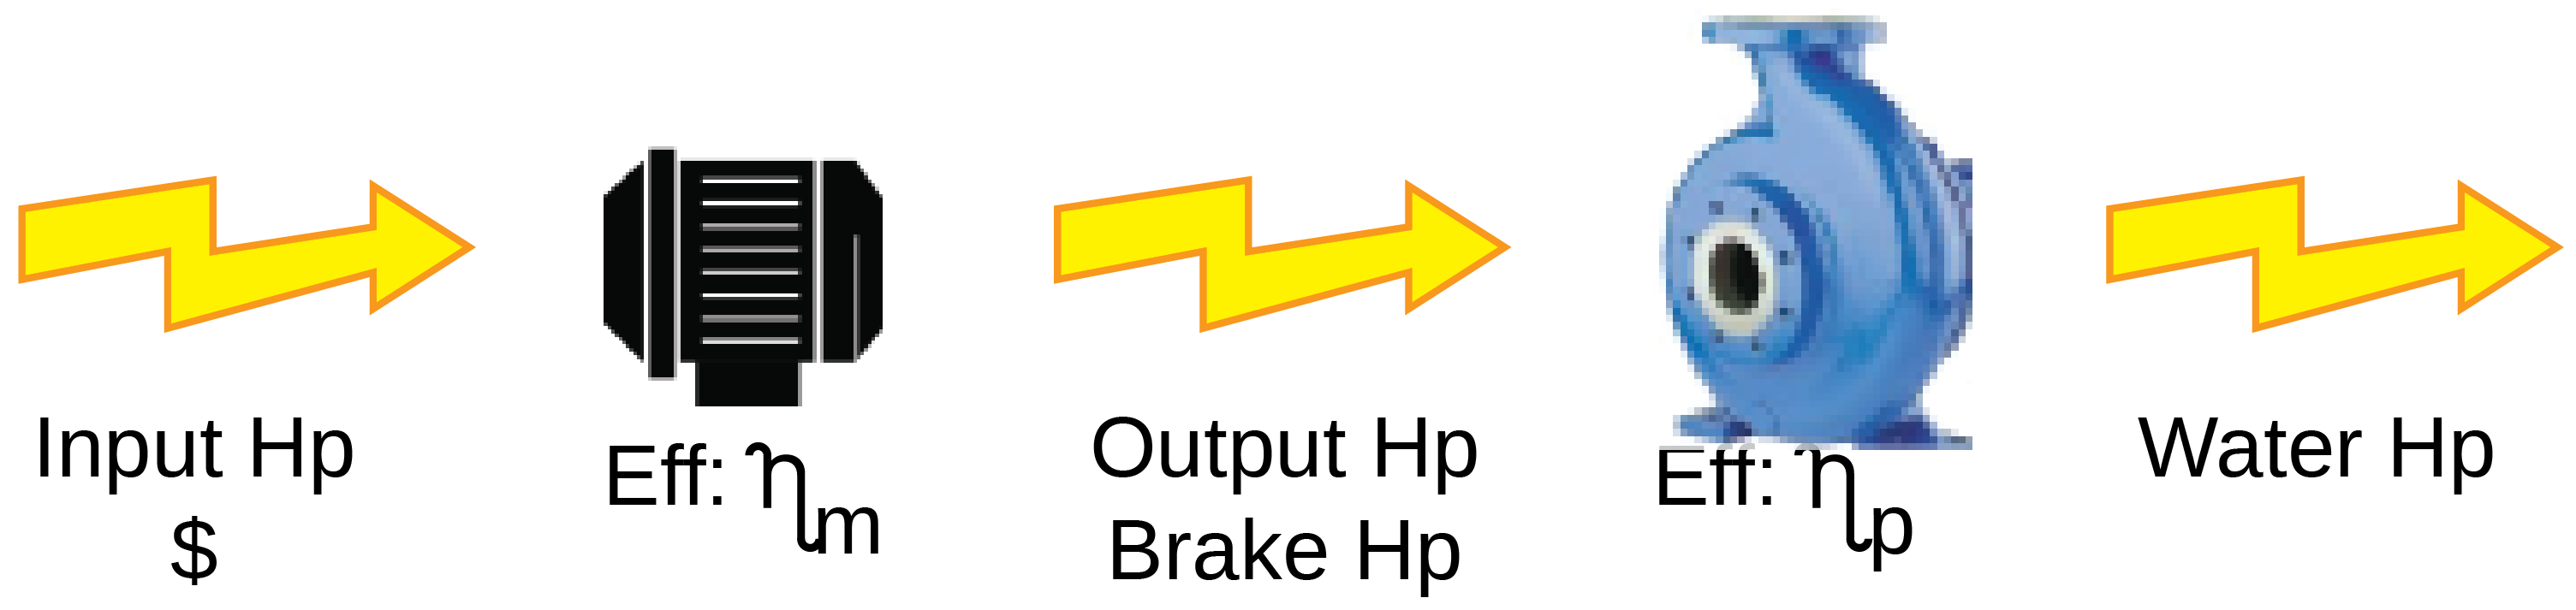
\includegraphics[scale=0.08]{PumpProblem}\\
 \vspace{0.2cm}
 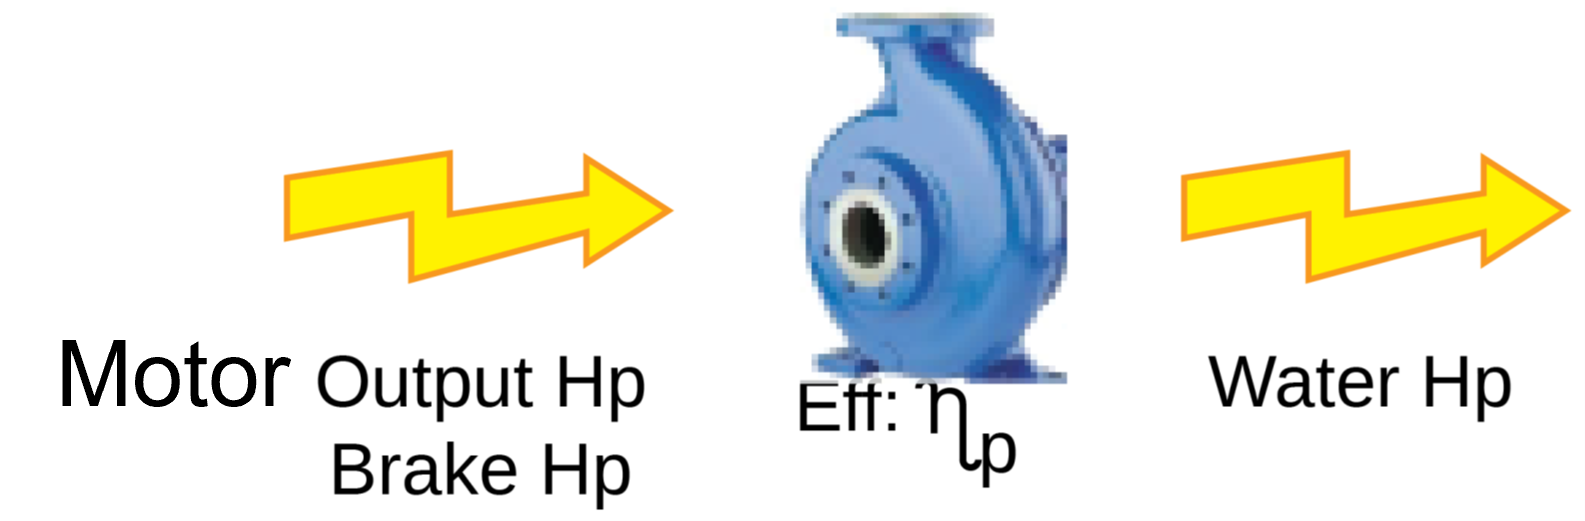
\includegraphics[scale=0.32]{PumpingProblemPump}
 \vspace{0.2cm}
$\dfrac{10 \mathrm{BHp}}{0.85}=\boxed{12 \mathrm{EHp \enspace or \enspace Input \enspace Hp}}$
 \vspace{0.4cm}


  Solution:\\ 
  \vspace{0.2cm}
 \vspace{0.08cm}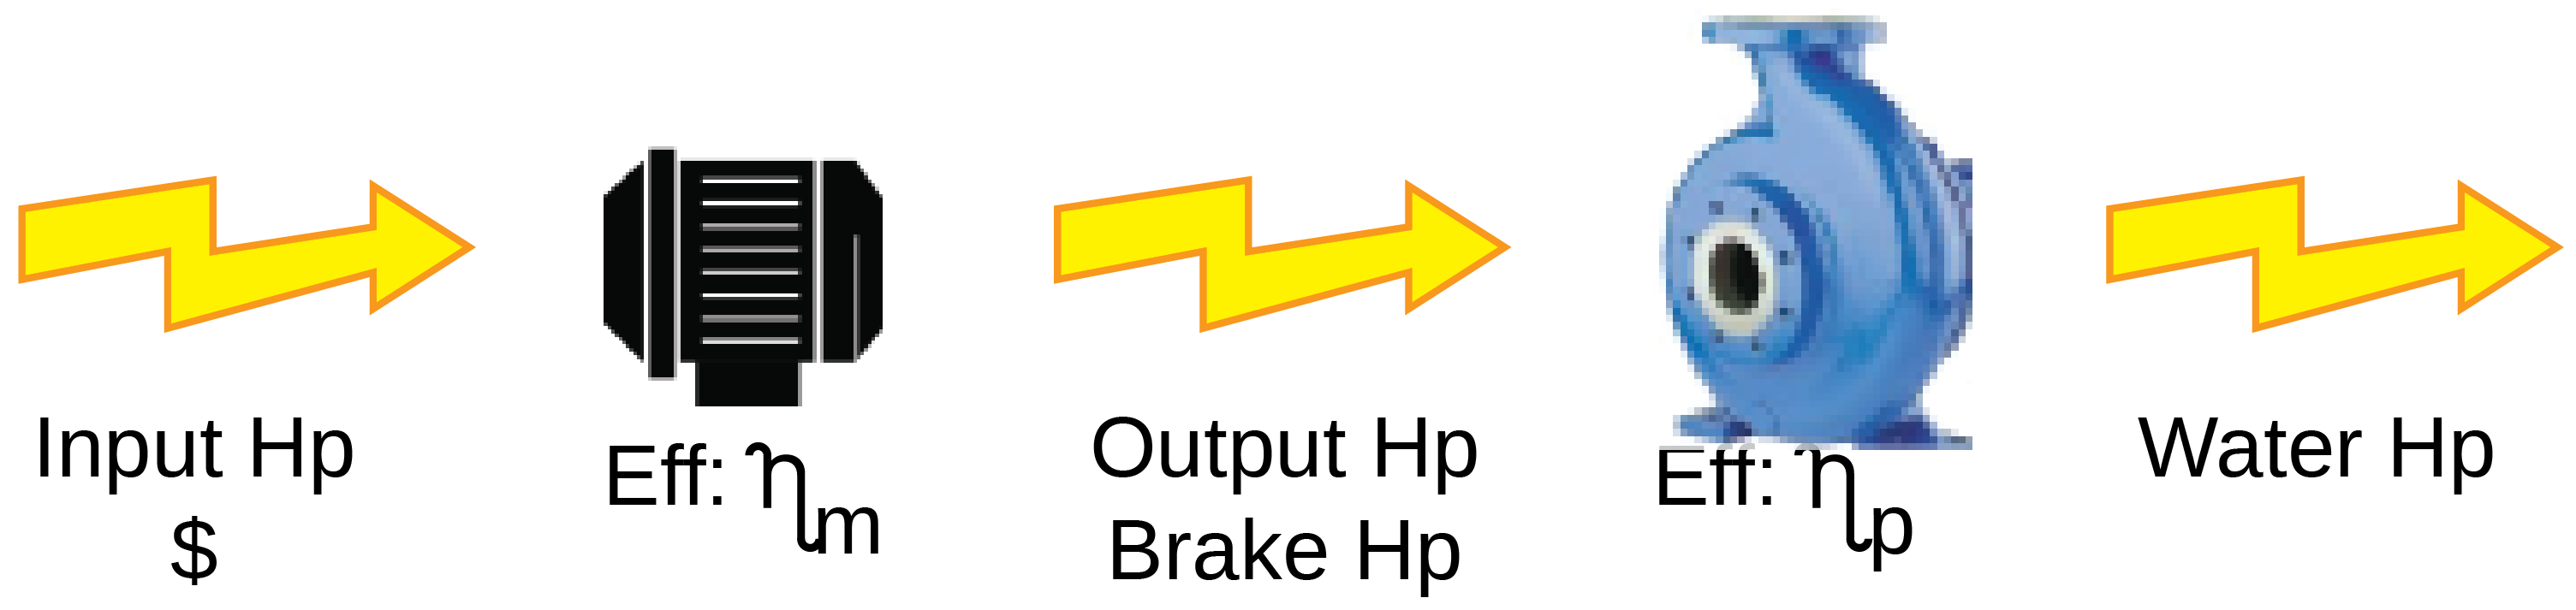
\includegraphics[scale=0.08]{PumpProblem}\\
 \vspace{0.2cm}
 \includegraphics[scale=0.32]{PumpingProblempump}
 \vspace{0.2cm}
$\eta_p=\dfrac{8.2 \mathrm{\enspace W \enspace Hp}}{10.3 \mathrm{\enspace BHp}} \times 100=\boxed{80 \%}$
 \vspace{0.2cm}


Solution:\\
\vspace{0.4cm}
water Hp = flow * head\\
\vspace{0.4cm}
$\mathrm{Water} \enspace \mathrm{Hp} = 120 \enspace \mathrm{gpm}*1,200 \enspace ft*\dfrac{\mathrm{Hp}}{3,960 \enspace \mathrm{gpm-ft}}=\boxed{ 37 \enspace \mathrm{Hp}}$\\
\vspace{0.2cm}


Solution:\\
\vspace{0.4cm}
$25 \enspace \mathrm{Hp}\dfrac{0.746 \enspace \mathrm{kW}}{\mathrm{Hp}}*\dfrac{8 \enspace \mathrm{hrs}}{\mathrm{day}}*\dfrac{7 \enspace \mathrm{days}}{\mathrm{month}}*\dfrac{\$0.07}{\mathrm{kWh}}=\boxed{\dfrac{\$73.1}{\mathrm{week}}}$\\
\vspace{0.2cm}

 Solution:\\
 \vspace{0.4cm}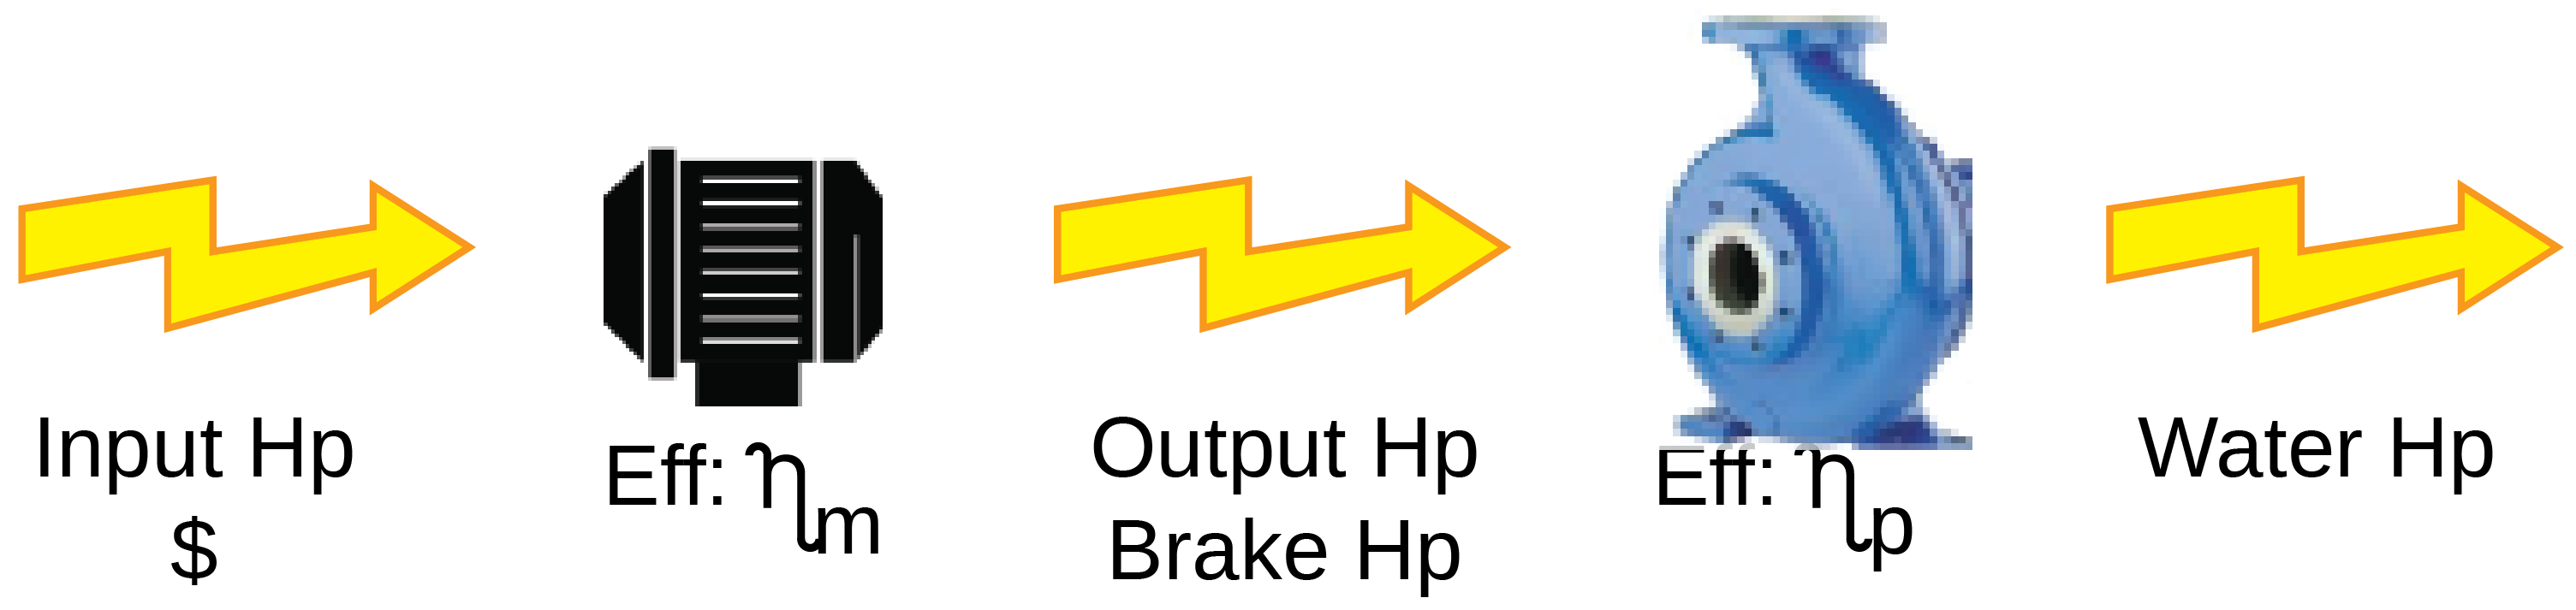
\includegraphics[scale=0.08]{PumpProblem}\\
 \vspace{0.2cm}
 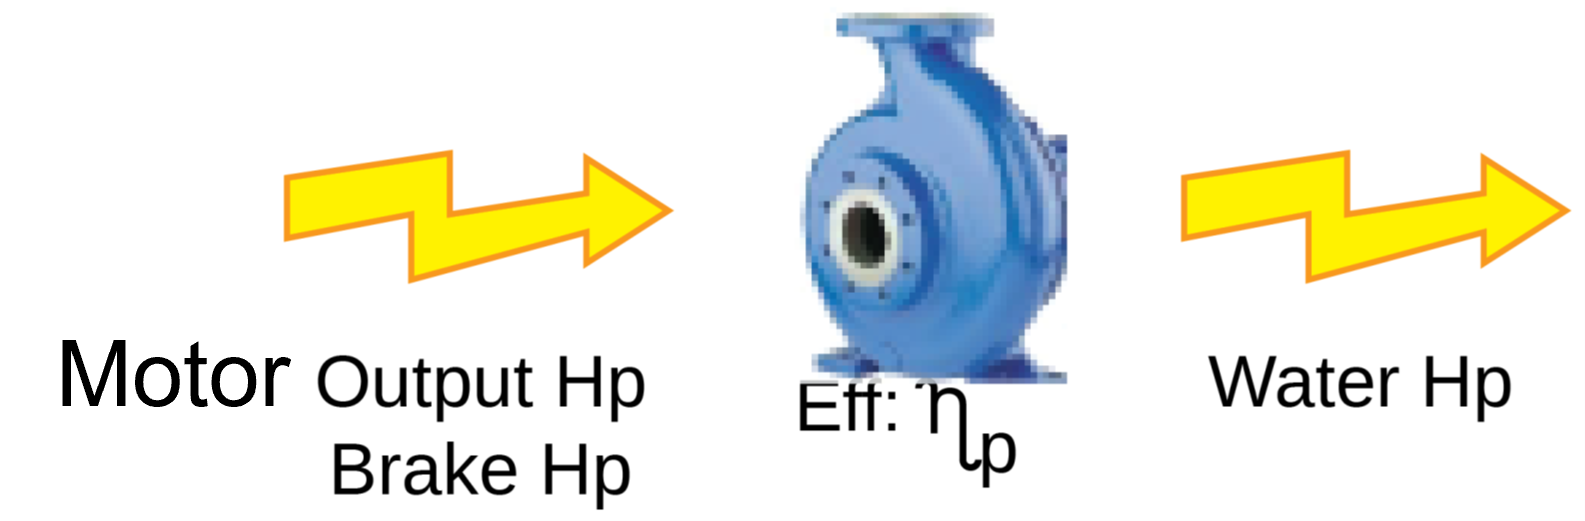
\includegraphics[scale=0.32]{PumpingProblemPump}
 \vspace{0.2cm}

water Hp = flow * head\\
 \vspace{0.2cm}
$\mathrm{Water} \enspace \mathrm{Hp} = 500 \enspace \mathrm{gpm}*50 \enspace ft*\dfrac{\mathrm{Hp}}{3,960 \enspace \mathrm{gpm-ft}}=\boxed{ 6.3 \enspace \mathrm{WHp}}$\\ 
  \vspace{0.2cm}
$\mathrm{Pump \enspace efficiency} =\dfrac{\mathrm{water \enspace Hp}}{\mathrm{brake \enspace Hp}} \implies \mathrm{brake \enspace Hp}=\dfrac{\mathrm{pump \enspace Hp}}{\mathrm{Pump \enspace efficiency}}$ \\
  \vspace{0.2cm}
$\textrm{brake} \enspace Hp = \dfrac{6.3}{0.85}=\boxed{7.4 \enspace \mathrm{Hp}}$\\
  \vspace{0.2cm}
$\mathrm{Motor \enspace efficiency} =\dfrac{\mathrm{brake \enspace Hp}}{\mathrm{input \enspace Hp}} \implies \mathrm{input \enspace \enspace Hp}=\dfrac{\mathrm{brake \enspace Hp}}{\mathrm{motor \enspace efficiency}}= \dfrac{7.4}{0.9}=\boxed{8.2 \enspace \mathrm{Hp}}$\\
  \vspace{0.2cm}
  
 \vspace{0.2cm}
$\mathrm{Wire-to-water} \enspace \mathrm{efficiency}=\eta_m * \eta_p \implies 0.9 \times 0.85 \times 100=\boxed{77 \%}$

 Solution:\\
\vspace{0.4cm}
water Hp = flow * head\\
$150 \enspace \mathrm{GPM}*75\mathrm{ft}*\dfrac{Hp}{3,960 GPM-ft}=\boxed{Water \enspace Hp = 2.8Hp}$\\
\vspace{0.4cm}
pump Hp = brake Hp * pump efficiency\\
$brake \enspace Hp = \dfrac{2.8}{0.9}=\boxed{Brake \enspace Hp=3.1Hp}$
 \vspace{0.2cm}




\section*{Practice Problems - Chemical Dosing}


  Determine the chlorinator setting in pounds per day if a water plant produces $300 \mathrm{gpm}$ and the desired chlorine dose is $2.0 \mathrm{mg} / \mathrm{L}$.

  The finished water chlorine demand is $1.2 \mathrm{mg} / \mathrm{L}$ and the target residual is $2.0 \mathrm{mg} / \mathrm{L}$. If the plant flow is $5.6 \mathrm{mgd}$, how many pounds per day of $65 \%$ hypochlorite solution will be required?

  Fluoride is added to finished water at a dose of $4 \mathrm{mg} / \mathrm{L}$. Find the feed rate setting for a fluoride saturator in gal/min if the water plant produces $5 \mathrm{mgd}$.

  If chlorine costs $\$ 0.21$ per pound, what is the daily cost to chlorinate a $5 \mathrm{mgd}$ flow rate at a dosage of $2.6 \mathrm{mg} / \mathrm{L}$ ?

  One gallon of sodium hypochlorite laundry bleach, with $5.25 \%$ available chlorine, contains how many pounds of active chlorine?

  How much sodium hypochlorite, in gallons, is required to obtain a residual of $100 \mathrm{mg} / \mathrm{L}$ in a well? The casing diameter is 18 -inches and the length is 80 feet. Sodium hypochlorite contains 5.25\% available chlorine. Assume a demand of $15 \mathrm{mg} / \mathrm{L}$.

  A water company uses an average of $600 \mathrm{gpm}$ of water. The water contains $0.30 \mathrm{mg} / \mathrm{L}$ of manganese and $0.06 \mathrm{mg} / \mathrm{L}$ of iron. How many pounds of iron and manganese are pumped into the distribution system each year?

  How many pounds of copper sulfate will be needed to dose a reservoir with $0.6 \mathrm{mg} / \mathrm{L}$ of copper? The reservoir holds 30 million gallons. The copper sulfate is $25 \%$ copper by weight.

  Liquid alum delivered to a water treatment plant contains $642.3$ milligrams of aluminum per milliliter of liquid solution. Jar tests indicate that the best alum dose is $9 \mathrm{mg} / \mathrm{L}$. Determine the setting on the liquid alum feeder in $\mathrm{ml} / \mathrm{min}$ when the plant flow is $3.2 \mathrm{mgd}$.

  The raw water supply contains $1.8 \mathrm{mg} / \mathrm{L}$ of fluoride. The flow rate is $400 \mathrm{gpm}$. The target fluoride dose for the finished water is $3 \mathrm{mg} / \mathrm{L}$. Find the desired feed rate in gpm for a fluoride saturator.

  The raw water alkalinity is $50 \mathrm{mg} / \mathrm{L}$ as calcium carbonate. The water is treated by adding 15 $\mathrm{mg} / \mathrm{L}$ of alum. What is the alkalinity of the finished water?



\section*{Practice Problems - Blending and Dilution}


Ferric chloride is being added as a coagulant to the raw water entering a plant. Sampling
shows that the concentration of ferric in the raw water is 25 ppm. A quick check of the chemical
metering pump shows that it is operating at a flow rate of 4.3 gpm. If the flow through the water
plant is 800 gpm, what is the concentration of raw chemical in the dosing tank?

A water plant is fed by two different wells. The first well produces water at a rate of 600
gpm and contains arsenic at 0.5 mg/L. The second well produces water at a rate of 350 gpm and
contains arsenic at 12.5 mg/L. What is the arsenic concentration of the blended water?

Liquid polymer is delivered as an 8 percent solution. How many gallons of liquid polymer
should be mixed in a tank to produce 150 gallons of 0.6 percent solution?

There are two raw water lines feeding a water plant. One line carries a flow rate of 500 gpm
with a TDS concentration of 1500 mg/L. The second line has a flow rate of 6 mgd with a a 250
mg/L TDS concentration. What is the actual combined TDS concentration entering the plant?


\textbf{Solutions:}\\

Solution:\\
\vspace{0.3cm}
\begin{tikzpicture}

\draw [-] (-3.2,4.2) -- (-0.4,4.2);
\draw [->] (-0.2,4) -- (-0.2,1.9);
\draw [->] (-3.2,1.9) -- (4,1.9);
\draw [shift={(-0.4,4)}] plot[domain=0:1.57,variable=\t]({1*0.2*cos(\t r)+0*0.2*sin(\t r)},{0*0.2*cos(\t r)+1*0.2*sin(\t r)});
\draw (-3.1,4.1) node[anchor=north west] {V$_{\tiny{FeCl_3}}$=$4.3 gpm$};
\draw (-3.1,3.6) node[anchor=north west] {C$_{\tiny{FeCl_3}}$ = ?};
\draw (-4.2,4.5) node[anchor=north west] {FeCl$_3$};
\draw (-4.2,2.2) node[anchor=north west] {Water};
\draw (-2.1,1.8) node[anchor=north west] {$800 gpm$};
\draw (0.7,1.8) node[anchor=north west] {C$_2$=25ppm FeCl$_3$};
\draw (0.7,1.3) node[anchor=north west] {V$_2$=4.3+800=804.3 gpm};
\end{tikzpicture}\\
\vspace{0.2cm}
C$_1$ * V$_1$ = C$_2$ * V$_2$ \\
\vspace{0.2cm}
C$_{\tiny{FeCl_3}}$ * V$_{\tiny{FeCl_3}}$  =  C$_2$ * (V$_{\tiny{FeCl_3}}$+V$_{\tiny{Water}}$)\\
\vspace{0.2cm}
C$_{\tiny{FeCl_3}}$ * 4.3 =  25 * (804.3)\\
\vspace{0.2cm}
C$_{\tiny{FeCl_3}}=\dfrac{25 * (804.3)}{4.3}=\boxed{4,676 \enspace \mathrm{ppm} \enspace \mathrm{or} \enspace 0.47\%}$\\
\vspace{0.3cm}

Solution:\\
\vspace{0.2cm}
C$_1$ * V$_1$ + C$_2$ * V$_2$ + =  C$_3$ * V$_3$=C$_3$*(V$_1$ + V$_2$)\\
\vspace{0.2cm}
C$_{Well \enspace 1}$ * V$_{Well \enspace 1}$ + C$_{Well \enspace 2}$ * V$_{Well \enspace 2}$ =  C$_{Blend}$ * V$_{Blend}$=C$_{Blend}$*(V$_{Well \enspace1}$ + V$_{Well \enspace 2}$)\\
\vspace{0.3cm}
$\implies C_{Blend}=\dfrac{C_{Well \enspace 1} * V_{Well \enspace 1} + C_{Well \enspace 2} * V_{Well \enspace 2}}{V_{Well \enspace 1} + V_{Well \enspace 2}}=\dfrac{0.5*600+12.5*350}{600+350}=\boxed{4.9 \enspace \textrm{mg/l}}$


Solution:\\
\vspace{0.5cm}
\begin{tikzpicture}[scale=1]
\draw[thick,-](-2,5) -- (0,5)node [at start, below,  black]{\small{}} node [anchor=north west, black]{} node [at start, left, black] (n){Water};;

\draw[thick,->](0,5)--(0,4.3) node [left,  black]{\small{}} node [anchor=north west, green]{} node [at start, above, red] (n){};
%\tikz\draw[line width=2mm] (0,0) -- (0,4);

\draw [<->] (2,1.9) -- (2,2.3) node [midway, midway] {};

\draw [<->] (-2,1.9) -- (-2,3.7) node [midway, midway] {};

\node [draw, cylinder, cylinder body fill=green, cylinder end fill=green!80, shape aspect=2, rotate=90, minimum height=1cm, minimum width=3cm] (c) at 
(0,3.8){};

%
\node [draw, cylinder, cylinder uses custom fill, cylinder body fill=black!10, 
cylinder end fill=black!10, shape aspect=2, rotate=90, minimum height=2cm, minimum width=3cm] (c1) at 
(0,2.8){};
%

\node [draw, cylinder, cylinder uses custom fill, cylinder body fill=black!30, 
cylinder end fill=black!10, shape aspect=2, rotate=90, minimum height=0.5cm, minimum width=3cm] (c1) at 
(0,2){};

\draw (2.2,2.6) node[anchor=north west] {C$_{1}$=8\%};

\draw (2.2,2.2) node[anchor=north west] {V$_{1}$=?};

\draw (-4,3.3) node[anchor=north west] {C$_{2}$=0.6\%};

\draw (-4,2.8) node[anchor=north west] {V$_{2}$=150 gal};



%\coordinate(dhtop) at ($(c1.after top)!-1*.1!(c1.before top)$);
%\coordinate(dhbot) at ($(c1.before bottom)!-1*.1!(c1.after bottom)$);
%\coordinate(dhlabel) at ($(dhtop)!.5!(dhbot)$);
%%\draw[|-|] (dhbot)--(dhtop);
%%\path (dhlabel) node[right, outer sep = 2pt] {$44'$};
%
%
%
%\coordinate(htop) at ($(c.before top)!-1*.1!(c.after top)$);
%\coordinate(hbot) at ($(c.after bottom)!-1*.1!(c.before bottom)$);
%\coordinate(hlabel) at ($(htop)!.5!(hbot)+(c.north)!.9!(c.center)$);
%
%\node [draw, cylinder, cylinder uses custom fill, cylinder body fill=black!20, 
%cylinder end fill=black!10, shape aspect=2, rotate=90, minimum height=1.5cm, minimum width=3cm] (c1) at 
%(0,-1.8){};
\end{tikzpicture}

\vspace{0.2cm}
C$_1$ * V$_1$ = C$_2$ * V$_2$ \\
\vspace{0.2cm}
V$_{1}$=$\dfrac{0.6*150}{8}=\boxed{11.25 \enspace \mathrm{gallons \enspace liquid \enspace polymer}} $\\
\vspace{0.3cm}


Solution:\\
\vspace{0.2cm}
C$_1$ * V$_1$ + C$_2$ * V$_2$ + =  C$_3$ * V$_3$=C$_3$*(V$_1$ + V$_2$)\\
\vspace{0.2cm}
C$_{Line \enspace 1 \enspace TDS} $ * V$_{Line \enspace 1}$ + C$_{Line \enspace 2 \enspace TDS}$ * V$_{line \enspace 2}$ =  C$_{Blend \enspace TDS}$ * V$_{Blend}$=C$_{Blend \enspace TDS}$*(V$_{Line \enspace1}$ + V$_{Line \enspace 2}$)\\
\vspace{0.3cm}
$\implies C_{Blend \enspace TDS}=\dfrac{C_{Line \enspace 1 \enspace TDS} * V_{Line \enspace 1 \enspace TDS} + C_{Line \enspace 2 \enspace TDS} * V_{Line \enspace 2}}{V_{Line \enspace 1} + V_{Line \enspace 2}}$\\
\vspace{0.3cm}
$\implies \dfrac{1500*\Big(\dfrac{500 \enspace gal}{min}*\dfrac{MG}{1,000,000 \enspace gal}*\dfrac{1440 min}{day}\Big)+6*250}{\Big(\dfrac{500 \enspace gal}{min}*\dfrac{MG}{1,000,000 \enspace gal}*\dfrac{1440 min}{day}\Big)+6}=\boxed{384 \enspace \textrm{mg/l}}$



\section*{Practice Problems - Sedimentation}


A circular clarifier has a diameter of 80 ft. If the flow to the clarifier is 1800 gpm, what is the surface overflow rate in gpm/ft

A sedimentation basin 70 ft by 25 ft receives a flow of 1000 gpm. What is the surface overflow rate in gpm/ft$2$?


A circular clarifier receives a flow of 3.55 MGD. If the diameter of the weir is 90 ft, what is the weir loading rate in gpm/ft?


\textbf{Solution}

$\mathrm{Surface \enspace overflow \enspace rate}=\dfrac{\mathrm{Flow, \enspace gpm}}{\mathrm{Clarifier \enspace surface \enspace area, \enspace ft}^2}=\dfrac{1,800 \enspace \mathrm{gpm}}{(0.785*80^2 )\mathrm{ft}^2}=\boxed{0.36 \enspace \mathrm{gpm/ft}^2}$

\vspace{0.2cm}
$\mathrm{Surface \enspace overflow \enspace rate}=\dfrac{\mathrm{Flow, \enspace gpm}}{\mathrm{Clarifier \enspace surface \enspace area, \enspace ft}^2}=\dfrac{1,000 \enspace \mathrm{gpm}}{(70 \mathrm{ft} \enspace * 25 \mathrm{ft})\mathrm{ft}^2}=\boxed{0.6 \enspace \mathrm{gpm/ft}^2}$

\vspace{0.2cm}
$\mathrm{Weir \enspace overflow \enspace rate}=\dfrac{\mathrm{Flow, \enspace gpm}}{\mathrm{Weir} \enspace \mathrm{length} \enspace ft}$\\
\vspace{0.3cm}
$\implies \dfrac{ \dfrac{3.55 \enspace \mathrm{MG}}{\mathrm{day}}*\dfrac{1,000,000 \enspace \mathrm{gal}}{\mathrm{MG}}*\dfrac{\mathrm{day}}{1440 \enspace \mathrm{min}}}{ (3.14*90) \enspace \mathrm{ft}}=\boxed{2,465 \enspace  \mathrm{gpm/ft}}$\\
\vspace{0.3cm}
\textit{Note: The concentration and volume (or flow) units need to be the same.  Thus, the gpm flow rate of Line 1 was converted to math the MGD flow rate unit of Line 2.}







\section*{Practice Problems - Filtration}

	At an average flow of 4,000 gpm, how long of a filter run in hours would be required to produce 25 MG of filtered water?
	
	A filter is $40 \mathrm{ft}$ long by $20 \mathrm{ft}$ wide. During a test of flow rate, the influent valve to the filter is closed for 6 minutes. The water level drop during this period is 16 inches. What is the filtration rate for the filter in $\mathrm{gpm} / \mathrm{ft}^{2}$ ?\\

  A water plant has three filters. Each filter is 12 feet wide by 12 feet long. Find the hydraulic loading rate in gpm/sf when all three filters are on-line and the raw water enters the plant at $9.5$ mgd.

  A sand filter will be backwashed at a rate of $8 \mathrm{gpm} / \mathrm{sf}$. If the filter is 10 feet wide by 15 feet long, what will the filter backwash rise rate be in inches per minute?

  A series of filters must be backwashed. Each filter is 20 feet square. If the goal is to achieve a filter backwash rise rate of 30 inches per minute, what should the backwash rate be in gpm/sf?

  A water plant has 3 filters. The plant is currently treating $5 \mathrm{mgd}$. If each filter is 12 feet wide by 20 feet long, what is the minimum number of filters that should be placed into service to keep the hydraulic loading rate below 20 gpm/sf?

  Find the yield for a filter in lbs/hr/sf given the following information: Filter operates for 12 hours of each day and captures $95 \%$ of the influent solids. The solids load to the filter is 200 pounds per day. The filter is 40 feet square.

  Coagulated raw water contains $120 \mathrm{mg} / \mathrm{L}$ of total suspended solids. The water plant produces $2.0 \mathrm{mgd}$ and has two sand filters that are 20 feet wide by 20 feet long. If the filters operate 22 hours of each day and capture $99 \%$ of the coagulated solids, what is the filter yield in lbs/hr/sf? What is the filter yield total in pounds per day?

  A series of filters discharge into a combined effluent trough. The trough is 5 feet wide by 80 feet long. A weir runs the full length of the trough. If the water plant capacity is 2 mgd, what is the weir overflow rate in gpd/sf?



\textbf{Solution}


$Flow \enspace rate \enspace (gpm)=\dfrac{Total \enspace flow \enspace (gal)}{Filter \enspace run \enspace time \enspace (min)}$

\vspace{0.3cm}

$\implies Filter \enspace run \enspace time \enspace (min)=\dfrac{Total \enspace flow \enspace (gal)}{Flow \enspace rate \enspace (gpm)}$\\

\vspace{0.3cm}

$\implies Filter \enspace run \enspace time \enspace (hr)=25 \enspace MG*\dfrac{1,000,000 \enspace \cancel{gal}}{MG}*\dfrac{\cancel{min}}{4,000 \enspace \cancel{gal}}*60 \enspace \dfrac{hr}{\cancel{min}}=\boxed{104 \enspace hrs}$

The volume of the water dropped after the inlet valve was closed would be the filter flow rate.  Since the dimensions to calculate are in feet and inches, the volume needs to be converted from ft$^3$ to gallons\\
\vspace{0.2cm}
$\text{Filtration rate, } \mathrm{gpm} / \mathrm{ft}^{2} = 
\dfrac{(
40 \mathrm{ ft}*20 \mathrm{ ft} * 16 \mathrm{\cancel{in}}*
\dfrac{ft}{12 \enspace \cancel{in}}
)
\cancel{ft^3}*7.48 \enspace 
\dfrac
{gal}
{\cancel{ft^3}}}
{40 \enspace ft * 20 \enspace feet}= \boxed{1.7\enspace gpm/ft^2}$\\



A disease that can be transferred by water is\\
a. Gonorrhea\\
b. Malaria\\
c. Mumps\\
d. Typhoid\\

The most important factor to consider in locating a well site from the health point of view is\\
a. Anticipated yield\\
b. Availability of electric power\\
c. Distance from other wells\\
d. Vulnerability\\

If water is flowing in a 12 -inch diameter water main and is discharged into an 6 -inch diameter water main, the velocity will\\
a. increase about four times\\
b. Decrease about twice\\
c. Remain the same\\
d. Increase about twice\\

The primary purpose of pressure-reducing valves between water system pressure zones is to\\
a. Minimize surge\\
b. Reduce downstream pressure\\
c. Control flows\\
d. Reduce upstream pressure\\

  A well is acidized in order to\\
a. Disinfect the water\\
b. increase yield\\
c. Remove objectionable gasses\\
d. Remove disinfection by-products\\

 An acceptable means of corrosion control for relatively small systems is\\
a. Activated carbon \\
b. $\mathrm{pH}$ control\\
c. zeolite softening\\

A main break may cause low pressure in the distributions system, which in turn may result in\\
a. Contamination of the system by backsiphonage\\
b. "ice" formation in the pipes\\
c. Increase in chlorine residual\\
d. Water hammer\\

The primary origin of coliforms in water supplies is\\
a. Natural algae growth\\
b. Industrial solvents\\
c. Fecal contamination by warmi-blooded animals\\
d. Acid raid\\

The primary health risk associated with volatile organic chemicals.(VOCs) is\\
a. Cancer\\
b. Acute respiratory diseases\\
c. "blue baby" syndrome\\
d. Reduced 1.Q. in children $\sim$ |ead\\

Which of the following best describes the characteristics of chlorine when used for disinfection in drinking water?\\
a:--Colorless, flammable, heavier than air\\
b. Greenish-yellow, nonflammable, lighter than air\\
c. Greenish-yellow, flammable, lighter than air\\
(d.) Greenish-yellow, nonflammable, heavier than air\\

Why should you contact other area companies with underground utilities before starting an underground repair.job?\\
(6.) To determine if there have been recent excavations in that location\\
b.  To ask these companies to mark the location of their utilities in the area of the repair job\\
c. To see if they also have excavating to do in the area\\
d. To see if they will help route traffic while you are doing the repair job\\

The discharge rate of a piston-type pump\\
a. Is constant as the main drive rpm changes\\
b. Is constant at a constant speed\\
c. Varies inversely with the head\\
d. Varies with the total dynamic head\\

Which of the following best describes "chlorine demand"?\\
a. The difference between the amount of chłorine added and turbidity\\
b. The difference between the amount of chlorine added and $\mathrm{pH}$\\
c. The difference between the total chlorine residual and the free chlorine residual\\
(d.) The difference between the amount of chlorine added and the amount of residual chlorine remaining after a given contact time\\

Which of the following chemicals will most likely keep iron in suspension?\\
a. Chlorine\\
b. Fluoride\\
c. Polyphosphate\\
d. Lime inhibitor 

The term "primacy" means the\\
a. Authority by the states to supersede USEPA drinking water regulations\\
b. Authority by the USEPA to supersede state drinking water regulations\\
c. Requirements for states to maintain drinking water regulations more stringent than USEPA regulations Primary authority for implementation and enforcement of drinking water regulations\\

Check valves are used to prevent\\
a. Excessive pump pressure\\
b. Priming\\
c. Water from flowing in two directions\\
d. Water hammer\\

Lead in drinking water can result in\\
a. Impaired mental functioning in children\\
b. Prostate cancer in men\\
c. Stomach and intestinal disorders\\
d. Reduced white blood cell count\\

The flow of electrical current is measured in\\
a. Amperes\\
b. Ohms\\
c. Volts\\
d. Watts 

$\mathrm{pH}$ is a measure of :\\
a. conductivity\\
b. water's ability to neutralize acid\\
c.  hydrogen ion activity\\
d. dissolved solids\\

An operator hears a pinging sound coming from the pump. What is the probabie cause?\\
a. Descaling\\
b. Cavitation\\
c. Corrosion\\
d. Hardness\\


Small gaseous chlorine leaks in and around a chlorinator can be detected by the use of commercial strength\\
a. Ammonia $\div \mathrm{Ntg}$. 
b. Hypochlorite $-$\\
c. Lime2\\
d. Soda ash\\

During a routine inspection on a centrifugal pump, the operator notices that the bearings are excessively hot. This is most likely caused by\\
a. Overiubrication\\
b. The speed being too slow\\
c. A worn impelier\\
d. A worn packing\\

Killing of pathogenic organisms in water treatment is called\\
a. Disinfection\\
b. Oxidätion\\
c. Pasteurization\\
d. Sterilization\\

The only acceptable breathing device to wear while handling chlorine leaks is the\\
a. Activated carbon canister type\\
b. Potassium tetroxide canister type\\
c. Self-contained breathing apparatus\\
d. Oxygen supply apparatus\\

The-leakage of seal-water around the packing on a centrifugal pump is required because it acts as a(n)\\
a. Adhesive\\
b.  Coolant\\
c. Corrosion inhibitor\\
d. Scale inhibitor\\

The letter or units "gpm" appearing on a flow rate indicator in a pumping station mean\\
a. Gallons per man\\
b. Gallons per man-hour\\
c. Gallons per mile of pipe\\
(d. Gallons per minute\\

Sodium Hypochlorite is\\
a. A commercially available chlorine solution\\
b. A commercially available dry chlorine compound\\
c. Chlorine that is available in 100- and 150-pound cylinders\\
d. A reaction product of chlorine and caustic soda\\

If raw water turbidity changed from 10 to 300 turbidity units and the finished water turbidity had increased from $0.1$ to 1.0 turbidity units, the unit process having the most impact to correct this situation is\\
a. Coagulation\\
b. Sedimentation\\
c. Filtration\\
d. Disinfection 37. Sodium Thiosulfate is used to\\
a. Buffer chlorine solutions\\
b.) Neutralize chlorine residuals\\
d. Sterilize sample bottles\\

The presence of total coliforms in drinking water indicates\\
a. The presence of pathogens.\\
b. The absence of an adequate chlorine residual\\
c. The existence of ann urigient public health problem\\
d. The potential presence of pathogens\\

A hypochlorinator is\\
a. Used to measure residual chlorine\\
b. Used in the treatment of iron and turbidity\\
c. Used to feed a liquid solution into a water supply\\
d. Used to measure an adequate amount of chlorine gas into the supply\\

The problem caused by dissolved carbon dioxide in the water of the distribution system is\\
b.  Corrosion\\
c. Excessive encrustation\\
d. Tastes and odors\\
a. increased trihalomethanes (THMs)\\

The water table is defined as the\\
a. Pumping water level in a well\\
b.  Upper surface of the groundwater\\
c. Water level in a reservoir\\
d. Bottom of the aquifer\\

A primary health risk associated with microorganisms in drinking water is\\
a. Cancer\\
b.) Acute gastrointestinal diseases\\
c. Birth defects\\
d. Nervous system disorders\\
GAC - TasteA odur green Sand fitter: In \& My\\

The granular filtration process is designed to reduce\\
a. Calcium and magnesium sulfates\\
b. True color\\
c. Total dissolved solids\\
d. Turbidity 44. A major health risk associated with nitrites and nitrates is\\
a. Cancer\\
b. Acute respiratory diseases\\
c.  "blue baby" syndrome\\
d. Reduced I.Q. in children CDPH MCL for $\mathrm{NO}_{3}-45 \mathrm{mg} / \mathrm{L}$ as $\mathrm{NO}_{3}$ lomgh as $\mathrm{N}$\\
$\mathrm{Na}+\mathrm{mg} / \mathrm{L}$\\

A primary source of volatile organic chemical (VOC) contamination of water supplies is\\
a. Agricultural pesticides\\
b.  Industrial solvents\\
c. Acld rain\\
d. Agricultural fertilizers\\

The presence of the coliform group of bacteria in water indicates\\
a. Contamination\\
b. Inadequate disinfection\\
c. Improper sampling\\
d. Taste and odor problems\\

It is essential to ventilate a vault before entry in order to\\
a. Rennove exçessive moisture\\
b. Equalize temperature and pressure\\
c. Eliminate foul odors\\
d. Remove dangerous gasses\\

After 5 years use, a portion of cast iron pipe shows a white scale about $1 / 2$ inch thick lining the inside. This means\\
a. Red water will soon become a problem\\
b. The water has been corrosive\\
c. The water is chemically unstable and is depositing\\
d. Water should flow easier since the lining is smooth\\

When calcium hypochlorite is used for disinfecting a water supply, it should be\\
a. Dissolved in water, allowed to settle, and the supernatant siphoned off and fed into the water system\\
b. Dissolved in water as a dry chemical then injected into the water system\\
c. Fed as a dry chemical directly into the pipeline\\
d. Fed as a dry powder into the clear well\\

The term "surface runoff" refers to\\
a. Rainwater that soaks into the ground\\
b. Rain that returns to the atmosphere from the earth's surface\\
c. Surface water that overflows the banks of rivers\\
d. Water that flows into rivers after a rainfall \\

Aeration in water treatment plants is used to\\
a. Lower the $\mathrm{pH}$\\
b. Reduce concentrations of dissolved gasses\\
c. Reduce turbidity\\
d. Stabilize chlorine residuals\\

What can the operator do if iron fouling appears to be a problem in an ion exchange softener?\\
a. Decrease the strength of the brine used in the regeneration stage\\
b. Increase backwash flow rates\\
c. Inçrease durattion of bacckwash stage\\
d. Increase duration of service stage\\

The peak capacity of water mains is often reduced by\\
a. High pressure\\
b. Looping\\
c. Tuberculation\\
d. Vacuum breakers\\

To protect stored water from contamination, a ground storage reservoir should\\
a. Be totally airtight\\
b. Have both the overflow pipe and vent screened\\
c. Have cathodic protection\\
d. Have its interior surface coated with an AWWA-approved paint system\\

An operator uses to test for residual chlorine\\
a. DPD\\
b. Cresol red\\
c. Methyl orange\\
d. Sulfuric acid\\

The purpose of monitoring requirements for unregulated contaminants is to\\
a. Provide the USEPA with more information to establish maximum contaminant levels (MCLs) for these contaminants\\
b. Assist the USEPA in determining the extent of source water contamination with these contaminants\\
c. Assist the USEPA in evaluating the need for future regulations\\
(d.) All of the above\\

The term "maximum contaminant level goal (MCLG)" means the\\
a. Maximum allowable level of a given contaminant in drinking water\\
b.  Level of a contaminant in drinking water below which there are no known or suspected adverse health effects with a margin of safety\\
c. Level of a contaminant in drinking water that will trigger a tier 1 violation\\
d. Minimum detectable level of a given contaminant 

The aeration process tends to decrease all of the following except\\
a. Carbon dioxide\\
b. Dissolved oxygen\\
c. Hydrogen sulfide\\
d. Volatile organic chemicals\\

Which of the following forms of iron is most soluble in water?\\
a. Ferric $\left(\mathrm{F}^{+3}\right)$\\
b. Ferric hydroxide $\left[\mathrm{Fe}\left(\mathrm{OH}_{3}\right)\right]$\\
d. Ferrous oxide (FeO)\\

At what $\mathrm{pH}$ would a chlorinated water have the highest concentration of hypochlorous acid?\\
a. 5\\
b. 7\\
c. 9\\
d. 11\\

Hydrogen sulfide gas causes\\
a. Corrosion of structures and equipment\\
b. High $\mathrm{pH}$ values\\
c. Destruction of algae\\
d. Destruction of bacteria\\

Positive displacement pumps should be operated when\\
a. Suction and discharge line valves are closed\\
b.  Suction and discharge line valves are open\\
c. Suction line valves are closed and discharge line valves are open\\
d. Suction tine valves are open and discharge line valves are closed\\

Turbidity in water can be caused by\\
a. Adequate filtration\\
b. .Dissolved gasses\\
c. Inadequate baffling\\
d. Unsettled particulate matter\\

The meniscus on calibrated glassware is read at the\\
a. Bottom of curvature for mercury but the top for water\\
b. Extreme point of contact between the liquid and glass, i.e., where gas, liquid, and air all meet at one point\\
c. Mid-height of the curvature so that beginning and ending readings will results in zero error\\
d. Top of curvature for mercury but at the bottom for most other liquids including water\\

An atmosphere is considered oxygen deficient when the oxygen level is below\\
a. $21.5 \%$\\
b. $20 \%$\\
c. $19.5 \%$\\
d. $17 \%$ 

Fluoride is generally added to public water supplies to\\
a. Aid in disinfection\\
b. Reduce pipe corrosion\\
c. Help prevent contamination\\
d. Protect the dental health of young citizens\\

As long as the temperature is steady, the pressure indicator on a chlorine cylinder will until all the chlorine has been gasified\\
a. Remaln steady\\
b. Decrease slowly\\
c. Decrease rapidly\\
d. Increase slightly\\

The component of a centrifugal pump sometimes installed on the end of the suction pipe in order to hold priming is the\\
a. Casing\\
b. Foot valve\\
c. Impeller\\
d. Lantern ring\\

A method used to soften water is\\
a. Aeration\\
b. Sedimentation\\
c. Ion exchange\\
d. Adsorption\\

Because chlorine residual is related to the $\mathrm{pH}$ of the water, it may be said that\\
a. A higher $\mathrm{pH}$ requires a higher chiorine residual\\

A higher $\mathrm{pH}$ requires a lower chlorine residual\\
c. A lower pH requires a higher chlorine residual\\
d. A lower $\mathrm{pH}$ has no effect on chlorine residual\\

At a pumping station equipped with centrifugal pumps, what can cause the discharge pressure to suddenly increase and the discharge quantity to suddenly decrease?\\
a.  A discharge valve was closed\\
b. A suction valve was closed\\
c. The pump amperage was decreased\\
d. The voltage was suddenly increased\\

Breakpoint chlorination is achieved when\\
a. Free ammonia can be tasted in the water\\
b. No chlorine residual is detected\\
c. The strong chlorine tasted at the plant did not persist in the distribution system\\
d. When chlorine dosage is increased, a corresponding increase in residual is detected\\

During a confined space entry, how often must the confined space be monitored for hazardous atmospheres?\\
a. Continuously\\
b. Every five minutes\\
c. Before entry only\\
d. Before entry and then once per hour during entry\\

The least amount of head loss in a pipeline would be caused by a fully open\\
a. Angle valve\\
b. Check valve\\
c. Gate valve\\
d. Globe valve\\

The maximum contaminant level goal (MCLG) of known or probable carcinogens is\\
a. Set by the state\\
b. The same number as the maximum contaminant level $(\mathrm{MCL})$\\
c. Zero\\
d. The minimum detectable level of a given contaminant\\

The proper emergeney repair kit for a ton chlorine cylinder is an\\
a. Emergency kit $A$\\
b. Emergency ikit B\\
c. Emergency kit C.\\
d. Emergency int $\mathrm{T}$\\

What is the only type of self-contained ireathing apparatus that should be used at water plants?\\
a. Negative-pressure\\
b. Zero-pressure\\
c. Positive-pressure\\
d. Air-pressure\\

The use of ammonia solution on a chiorine gas leak from the disinfection assembiy may cause which of the following?\\
a. Explosion\\
b. Hydrochloric acid\\
c. Toxic gases\\
d. Dense white smoke\\

Which of the following substances pose on immediate health threat whenever otandards are exceeded?\\
a. Benzene and mereury\\
b. Coliform and nitrate\\
c. Nercury andi coliform\\
d. Lead and nitrate\\

Ozone contactors must have a system to collect ozone off-gas because ozone is\\
a. Toxic\\
b. Explosive\\
c. Mutagenic\\
d. Magnetic.\\

What is the causative organism for cholera?\\
a. Vibrio\\
b. Shigella\\
c. Yersinia\\
d. Mycobacterium\\

Which health effect category refers to an organic chemical that is a known carcinogen?\\
a. Category I\\
Đ. Category II\\
c. Category III\\
d. Category IV\\

A room measures $12 \mathrm{ft}$ high, 30 ft long, and 17 ft wide. How many cubic feet per minute of air must a blower in an air exchange unit move to completely change the air every 10 minutes?\\
a. 102\\
b. 612\\
c. 1,020\\
d. 6,120\\

One volume of liquid chlorine gas will expand, at room temperature and pressure, to occupy how many volumes of gas?\\
a. 16 volumes\\
b. 46 volumes\\
c. 460 volumes\\
d. 960 volumes\\

What is the odor detection limit of chlorine gas?\\
a. $0.1 \mathrm{ppm}$\\
b. $0.3 \mathrm{ppm}$\\
c. $0.6 \mathrm{ppma}$\\
d. $1.0 \mathrm{ppm}$\\

$$10 / 03 / 19$$\\

If a trench is $526 \mathrm{ft}$ long, $4.0 \mathrm{ft}$ wide, and $5.5 \mathrm{ft}$ deep, how many cubic yards of soil were excavated?\\
$$526 \times 4 \times 5.5=\frac{11,572 \mathrm{f}^{3}}{27}=428$$\\

If exactly $100 \mathrm{gal}$ of polymer costs $\$ 19.50$, what will $5,500 \mathrm{gal}$ cost, assuming no quantity discount?\\
$$\frac{19.50}{100} \times 5500=1,072.5$$\\

What is the velocity of flow in feet per second for an 8.0-in. diameter pipe if it delivers 675 gprax?\\
$$\frac{150}{6.35}$$\\

$$\frac{675}{449}=15 \mathrm{cuft} / \mathrm{s}$$\\

$$\begin{aligned} & 430 \mathrm{ft} / \mathrm{s} \end{aligned}$$\\

What should the setting be on a chlorinator in pounds per day if the dosage desired is $2.90 \mathrm{mg} / \mathrm{L}$ and the pumping rate from the well is $975 \mathrm{gpm}$ ?\\
$$\frac{975}{69)^{1}}=1.4 MGD $$\\
$$1.4 \times 8.34 \times 2.90$$\\

A treatment plant uses $278 \mathrm{lb} / \mathrm{d}$ of chlorine gas. If the chlorine demand is $0.85 \mathrm{mg} / \mathrm{L}$ and the chlorine residual is $1.50 \mathrm{mg} / \mathrm{L}$, how many million gallons per day are being treated?\\
$$\frac{278}{8.34 \times 2 \times 35}=$$\\
$$\text { dojarge } ;$$\\
$$\begin{aligned}& 0.85+1.50= \\& 2.35 \mathrm{mg} / \mathrm{h}\end{aligned}$$\\

A water tank that is $105 \mathrm{ft}$ in diameter needs to be disinfected with a $5.0 \%$ sodium hypochlorite solution. If the tank is to be filled to only a depth of $5.0 \mathrm{ft}$ and the concentration required is $20.0 \mathrm{mg} / \mathrm{L}$, how many gallons of sodium hypochlorite are needed? Assume the sodium hypochlorite solution weighs 8.92 lb/gal.\\
$$\frac{0.323 M G P}{0.323 \times 8.34 \times 20}=$$\\
$$9 / 23 / 19$$\\

Convert $8.0 \mathrm{cfs}$ to $\mathrm{gpm}$.\\
a. $1.07 \mathrm{gpm}$\\
$\begin{array}{ll}\text { b. } 64.2 \mathrm{gpm} \\ \text { c. } 480 \mathrm{gpm} & 8 \times 449\end{array}$\\
(e.) $3,436 \mathrm{gpm}$\\

Conyert 4,000 gpm to cfs.\\
a.  $8.91 \mathrm{cfs}$\\
b. $66.65 \mathrm{cfs}$\\
c. $499 \mathrm{cfs}$\\
d. $535 \mathrm{cfs}$\\
e. $32,076 \mathrm{cfs}$\\

Convert $12 \mathrm{MGD}$ to gpm.\\
a. $0.00833 \mathrm{gpm}$\\
b. $7,200 \mathrm{gpm} \quad 12 \times 700$\\
d. $17,280 \mathrm{gpm}$\\
e. $199,992 \mathrm{gpm}$\\

Convert $5.5$ cfs to MGD.\\
a. $0.059 \mathrm{MGD}$\\
b. $0.148$ MGD\\
c. $0.475 \mathrm{MGD}$\\
(64) more Aaumole\\
e. 7,920 MGD\\

Convert 45 Acre-feet into million gallons.\\
a. $6.02 \mathrm{Mgal}$\\
b. $1.96 \mathrm{Mgal}$\\
c.  $14.7 \mathrm{Mgal}$\\
d. $45 \mathrm{Mgal}$\\
e. $336.6 \mathrm{Mgal}$\\

Convert $6.5$ feet per second into miles per hour.\\
a.  $4.43 \mathrm{mph}$\\
c. $13.3 \mathrm{mph}$\\
d. $106 \mathrm{mph}$\\
e. $266 \mathrm{mph}$\\

Convert $3.4$ miles into feet.\\
a. 5,000 feet\\
b. 5,280 feet\\
c. 5,984 feet\\
d. 10,000 feet\\
(e.) 17,952 feet\\
$$=\frac{6.5 / 5280}{1 / 60 \times 60}$$\\
$1 \mathrm{~m} / \mathrm{e}=25$ ft\\

Convert $2,250 \mathrm{gpm}$ into MGD.\\
a. 0.054MGD\\
b. $3.24 \mathrm{MGD}$\\
d. $2,250 \mathrm{MGD}$\\
e. 3,240 MGD\\

Convene $9.75 \mathrm{MGD}$ into cfs.\\
a.  $15.1 \mathrm{cfs}$\\
b. $37.75 \mathrm{cfs}$\\
c. $113 \mathrm{cfs}$\\
d. $363 \mathrm{cfs}$\\
e. $845 \mathrm{cfs}$\\
$$236 \pi$$\\

Convert $1,000,000$ cubic feet into Acre-feet.\\
a. $0.04356 \mathrm{AF}$\\
b. $0.325829 \mathrm{AF}$\\
c. $3.07 \mathrm{AF}$\\
d. $22.96 \mathrm{AF}$\\
e. $172 \mathrm{AF}$\\

The conversion of liquid water to gaseous water is known as\\
a. Condensation\\
b. Percolation\\
c.. Evaporation\\
d. Runoff\\
e. None of the above\\

A well is located in an aquifer with a water table elevation 20 feet below the ground surface. After operating for three hours, the water level in the well stabilizes at 50 feet below the ground surface. The pumping water level is\\
a. 20 feet\\
b. 30 feet which represents a surface of zero pore pressure.\\
linconfind\\
aquifer\\
Prezometre surface 6 Pore pressure in a con frved aquifor:\\
e. 100 feet\\

The height to which water will rise in wells located in an artesian aquifer is called the\\
a. Pumping water level\\
b. Water table\\
W Arteíran aquifer is a con frued\\
c. Piezometric surface\\
d. Drawdown\\
e. Radius of influence aquifer under positire prasure.\\

What percentage of all the earth's water is readily available as a potential drinking water supply in the form of lakes, rivers, and near-surface ground water?\\
a. $97 \%$\\
b. $50 \%$\\
c. $2 \%$\\
d. $\quad 1 \%$\\
e. $0.34 \%$\\

To prevent the entry of surface contamination into a well is the purpose of\\
a. The well casing\\
b. The water table\\
c. The louvers or slots\\
d. Well development\\
The annular grout seal\\

An aquifer that is located underneath an aquiclude is called\\
a. An unconfined aquifer\\
c. A water table\\
d. Unreachable groundwater\\
e. An Artesian spring 7. The process by which water changes from the gas to the liquid phase is termed\\
$\begin{array}{ll}\text { a.  } & \text { Condensation } \\ \text { b. } & \text { Evaporation } \\ \text { c. } & \text { Percolation } \\ \text { d. } & \text { Precipitation } \\ \text { e. } & \text { Runoff }\end{array}$\\

The free surface of the water in an unconfined aquifer is known as the\\
a. Pumping water level\\
b. Artesian spring\\
c.) Water table:\\
d. Drawdown\\
e. Percolation\\

The transfer of liquid water from plants and animals on the surface of the earth into water vapor in the atmosphere is called\\
a. Transpiration\\
b. Evaporation\\
c. Condensation\\
d. Runoff\\
e. Percolation\\

The term for the combined processes which transfer liquid water on the earth's surface into water in the gas phase in the atmosphere is.\\
a. Percolation\\
b. Evapotranspiration\\
c. Sublimation\\
d. Overdraft\\
e. Precipitation\\

A water-bearing formation in the soil is referred to as-\\
a. An aquitard or aquiclude\\
b. An aquifer\\
c. An aqueduct\\
d. The drawdown\\
e. The static water level\\

An operating well will drain the water from a volume of soil around the well during pumping. This volume is referred to as the\\
a. Pumping water level\\
b. Radius of influence\\
c. Drawdown\\
d. Cone of depression\\
e. Recharge zone

The elevation of water in the casing of an operating well is called the\\
a. Piezometric surface\\
b. Water table\\
c. Pümping water level\\
d. Drawdown\\
e. Radius of influence\\

An aquifer under pressure is often termed\\
a. Unconfined\\
b. Pacific\\
c. Artesian\\

An aquifer is usually composed of bou cuator and dipositel in valleys.\\
a. Sand and gravel\\
b. Clays and silts\\
c. Bedrock\\
d. Large voids in the soil, resembling underground lakes\\
e. None of the above\\

The movement of water on the surface of the earth is called\\
a. Percolation\\
b. Evaporation\\
c. Evapotranspiration\\
d. Runoff\\
e. Infiltration\\

A formation in the soil that resists water movement (such as a clay layer) is called\\
a. An aquitard or aquiclude\\
b. An aquifer\\
c. An aqueduct - seestem of proes,drichs, canals to carry water auray\\
d. The drawdown\\
e. The static water level\\

Another term for the percolation that transports water from the surface into an aquifer is\\
a. Artesian springs\\
b. Recharge:\\
c. Extraction\\
d. Overdraft\\
e. Runoff 13. The elevation of the free surface in a water table well which is not running is termed\\
a. An aquifer\\
b. An aquitard or aquiclude\\
c. An aqueduct\\
d. The drawdown\\
e. The static water level\\

One acre is 43,560 square feet. If this acre is covered with one foot of water, it contains\\
a. $\quad 1$ acre-foot\\
b. 43,560 cubic feet\\
c. 325,829 gallons\\
d. All of the above\\
e. None of the above\\

The safe yield of an aquifer is\\
a. Determined by the Department of Health Services\\
b. Variable, depending on rainfall\\
c. The average amount of water that can be withdrawn each year without causing a long-term drop in the water table\\
d. The difference between the static water level and the pumping water level\\
e. All of the above\\

The movement of water from the surface of the earth into the soil is called\\
a. Condensation\\
b. Evaporation\\
c. Evapotranspiration\\
d. Runoff\\
e. None of the above :\\
L Perculation.\\

The freezing point of water is\\
a. $\quad 0^{\circ} \mathrm{F}$\\
b. $\quad 32^{\circ} \mathrm{C}$\\
r. $\quad 32^{\circ} \mathrm{F}$\\
d. $\quad 100^{\circ} \mathrm{C}$\\
e. $100^{\circ} \mathrm{F}$\\

The movement of water from the atmosphere to the surface of the earth is called\\
a. Condensation\\
b. Evaporation\\
c. Evapotranspiration\\
d. Runoff\\
e. Precipitation\\

The variation in water demand during the course of a day is termed\\
a. Seasonal variation\\
b. Fire flow requirements\\
c. Emergency storage variation\\
d. The straight line equalization method\\
e. Diurnal variation\\

The typical per capita water use per day in the United States is\\
a. $5-6$ gallons\\
b. $50-60$ gallons\\
c. $500-600$ gallons\\
d. $\quad 5000-6000$ gallons\\
(e.) None of the above\\

The maximum momentary load placed on a water supply system is known as\\
a. Average daily flow\\
b. Average daily demand\\
c. Rated capacity\\
d. System float\\
e.) Peak demand\\

Most below-ground-leve storage tanks are constructed of\\
b. Fiberglass\\
(d. Concrete :\\
e. Special composite materials\\

An unknown substance is found on the bottom of the water within a drinking water reservoir. Which of the following statements is true of this substance?\\
a. It has a specific gravity less than $1.0$\\
b. It has a specific gravity equal to $1.0$\\
c. It has a specific gravity greater than $1.0$\\
d. It has no specific gravity\\
e. None of the above\\

Elevated storage tanks are used primarily to\\
a. Eliminate the need for continuous pumping\\
b. Minimize variations in the system water pressures\\
c. Reduce auxiliary power requirements\\
d. Provide a considerable amount of water for storage\\
e. Protect against backflows 31. A valve that automatically shuts off flow into an elevated storage tank when the water level in the tank reaches a preset level is termed a(n)\\
a. Gate valve\\
b. Air / vacuum relief valve\\
c. Wet-barrel hydrant\\
d.  Altitude valve\\
e. Angle valve\\


A pressure gauge reads 100 psi. This is equivalent to\\
a. 43.3 feet\\
b. 110 psig\\
c. 2.31 feet\\
d. 231 feet\\
e. 231 psig\\

Because pipe materials come into contact with drinking water, they must conform with\\
a. Primary drinking water standards\\
b. Secondary drinking water standards\\
Surface water treatment rule\\
NSF - National Sanitation roundation\\
d.  ANSI/NSF Standard $61^{\prime}$\\
e.' All of the above ANs I - American National standand Institute\\

An example of a pipe material that is difficult to locate underground is\\
a. Mortar lined and coated steel\\
b. Reinforced concrete cylinder\\
c. Ductile iron\\
d. Asbestos-cement\\
e. Steel\\

The size of water mains, pumping stations, and storage tanks is primarily determined by\\
a. Fire protection requirements\\
b. The maximum 24-hour flow period recorded\\
c. Average per capita consumption rates\\
d. Maximum design velocity standards\\
e. Minimum design velocity standards\\

Ten (10) feet of head is equivalent to\\
a. $\quad 2.31 \mathrm{psi}$\\
b. $4.33 \mathrm{psi}$\\
c. $\quad 14.7 \mathrm{psi}$\\
d. $\quad 23.1 \mathrm{psi}$\\
e. $43.3 \mathrm{psi}$ 

Pipe with a "C" factor of 140 is regarded as having a(n)\\
a. Extremely smooth interior\\
b. Extremely rough interior\\
c. Extremely high corrosion resistance\\
d. Extremely low corrosion resistance\\
e. A purple color\\

What is the weight of 1 gallon of water?\\
a. 1 lb\\
b. 2.31 lbs\\
c. 7.48 lbs\\
d. 8.34 lbs\\
e. 62.4 lbs\\

Pressure is usually measured in\\
a. cfs\\
b. psi\\
c. MGD\\
d. GPM\\
e. Feet per second\\

The lowest point of the inside of a pipe is known as the\\
a. Pervert\\
b. Soffit\\
c. Invert\\
d. Curb stop\\
e. None of the above\\

A lightweight type of pipe that has a very smooth interior, is essentially corrosion-free, and which is difficult to locate when buried is\\
a.  Polyvinyl chloride : PVC\\
Cast iron\\
c. Ductile iron\\
d. Concrete cylinder\\
Steel\\

An example of a pipe material that is relatively easy to locate underground is\\
a. ABS\
b. PVC\\
c. Reinforced concrete cylinder\\
d. Asbestos-cement\\

Sleeve-type and "victaulic" couplings are the most common forms of\\
a. Mechanical couplings\\
b. Welded joints two topes: But pount \& socket jount\\
c. Asbestos-cement pipe fittings\\
d. PVC pipe fittings\\
e. Flanged joints - In a flonged eoupling / a flomge is welded to the each\\
of the pope and then two flanges are bolted. Thi toue is easrer to drsconmat prpes athen\\
a. Insert an eight-foot liner\\
b. Replace section and connect with solid sleeves or couplings\\
c. Use compression couplings to seal the crack\\
d. Wrap with epoxy tape\\
e. All of the above\\

If possible, a water main leak should be repaired under pressure to\\
a. Prevent contamination of the water line\\
b. Prevent flooding of basements\\
c. Save repair time\\
d. Use fewer materials\\
e. All of the above\\

A connection made into a main that is full or under pressure is called a\\
a. Cross connection\\
b. Dry tap\\
c. Valve box\\
d. Wet tap :\\
e. Spinal tap\\

The tensile strength of a pipe is its ability to\\
a. Stretch or pull without breakage\\
b. Resist internal pressure without breakage\\
c. Resist external pressure without breakage\\
d. Twist or bend without breakage\\
e. Resist heating without breakage\\

When is the best time to perform a distribution main flushing program?\\
a. During night hours, to minimize traffic and other customer concerns\\
b. During weekday day shift hours, to minimize overtime costs\\
c. During Summer months, due to high system velocities\\
d. During Spring months, prior to high system demands of Summer\\
e. None of the above\\

An system for the prevention of corrosion is called\\
a. Water hammer\\
b. Reverse osmosis\\
c. Diurnal variation\\
d. A foot valve\\
e. Cathodic protection.\\

What category of meters is exemplified by propeller and turbine types?\\
a. Differential pressure\\
(b) Positive displacement Mass flow\\
(d.) Velocity\\
None of the above\\

The hydraulic grade line in a pipeline is normally determined by\\
a. Reading pressure gauges\\
b. Checking for backflow\\
c. Opening fire hydrants on each loop of the system\\
d. Using a leak detector\\
e. A venturi meter\\

The slope of the hydraulic grade line is due to\\
a. Woll elevations\\
b. Elevations of storage facilities\\
c. Pumping\\
d. Backflows\\
e. Friction loss\\

A normally buried valve located on a street water main and leading to a water service is known as a\\
a. Check valve\\
b. Gate valve\\
c. Corporation stop\\
d. Altitude valve\\
e. Butterfly valve\\

The risk of pipeline damage from water hammer can be reduced by\\
a. Installation of gate valves\\
b. Air release valves\\
c. Repair of defective pipes\\
d. Trimming pump impellers\\
e. Rapid closing of pump discharge valves 

A venturi is a device used to\\
a. Increase water flow\\
b. Decrease water flow\\
c. Regulate water flow\\
d. Stop or start water flow\\
e. Measure water flow\\

The most commonly used meter on small diameter domestic service is the\\
a. Venturi meter\\
b. Propeller meter\\
c. Orifice plate meter\\
d. Compound meter\\
e. Nutating disc meter\\

The valve type most commonly used for isolation in a water distribution system is the\\
a. Gate valve\\
b. Air relief valve\\
c. Globe valve\\
d. Ball valve\\
e. Butterfly valve\\

The proper location for air relief valves is\\
a. At low points along a pipeline\\
b. At high points along a pipeline\\
c. At the bottom of surge tanks\\
d. At the mid-line of water storage reservoirs\\
e. At the springline of a pipeline\\

When fully open, which of the following will have the highest friction loss?\\
a. Gate valve\\
b. Butterfly valve\\
c. Globe valve\\
d. Ball valve\\
e. All will have about the same friction loss.\\

Which of the following is a device used to measure flow?\\
a. Baffle\\
b. Diversion box\\
c. Stop logs\\
d. Weir\\
e. None of the above 61. A compound meter is a device which\\
a. Is installed to allow automated meter reading\\
b. Can be installed to measure water use by as many as 12 separate customers\\
c. Provides accurate readings over a wide range of flows\\
d. Electronically records peak flows, as a demand meter does for electricity\\
e. Is a typical residential water flow meter\\

Magnetic flow meters and ultrasonic flow meters are well suited to measure flow rates of water with a large concentration of suspended solids, because they have\\
a. The best accuracy of any meters\\
b. No parts within the flow stream\\
c. Easily accessed cleanout ports\\
d. Simple recalibration procedures\\
e. All of the above\\

A nutating disk is found in certain\\
a. Centrifugal pumps\\
b. Positive displacement pumps $*$\\
c. Main line valves\\
d. Chemical feeders\\
e. Water meters\\

The most common valve in a water distribution system is the\\
a. Gate valve\\
b. Air relief valve\\
c. Globe valve\\
d. Ball valve\\
e. Butterfly valve\\

The drain hole in a fire hydrant is designed to\\
a. Release air upon closing the valve\\
b. Relieve vacuum upon opening the valve\\
c. Allow access for interior inspection\\
d. Relieve excess water pressure when closing the valve\\
e. Remove water from the riser to prevent freezing\\

A typical installation site for a compound meter is\\
a. Any small commercial business\\
b. A common single location with as many as 12 separate customers\\
c. A large industrial user\\
d. Any location that requires the electronic monitoring of peak flows\\
e. A typical residential water flow meter 

An example of a pressure-differential type water meter is a\\
a. Venturi meter\\
b. Propeller meter\\
c. Nutating disk meter\\
d. Magnetic flow meter\\
e. Utrasonic flow meter\\

When closing a hydrant, it should be\\
a. Closed rapidly to minimize water loss\\
b. Closed slowly to reduce surges\\
c. Closed using a standard valve key\\
d. Closed using a standard pipe wrench\\
e. Closed at the street valve and left slightly open at the hydrant valve\\

Dry-barrel fire hydrants have their operating valves\\
a. In the base\\
b. In the head\\
c. Either of the above, depending on the manufacturer\\
d. In the street several feet away from the riser\\
e. None of the above\\

An example of a valve that has a 90 degree travel is a\\
a. Butterfly valve\\
b. Plug valve\\
c. Ball valve\\
d. All of the above.\\
e. None of the above\\

The valve type most commonly found on the discharge of a pump or well, and installed to prevent reverse flows is the\\
a. Gate valve\\
b. Check valve\\
c. Globe valve\\
d. Butterfly valve\\
e. Ball or Plug valve\\

Features that impact the " $K$ "' factor for measuring friction in pipelines include\\
a. Pipe length\\
b. Pipe type\\
c. Number of valves\\
d. Type of valves\\
e. All of the above\\

In an occupied trench where exits (i.e., ladders) are required, what is the maximum allowed travel distance between an occupant and the nearest exit?\\
i. 25 feet\\
b. 50 feet\\
c. 100 feet\\
d. At the discretion of the safety officer\\
e. None of the above\\

Standard first aid procedures direct that the first step to control bleeding is to\\
a. Apply a tight tourniquet\\
b. Apply pressure directly to the wound\\
c. Let it bleed until natural clotting takes place\\
d. Wash wound and bandage\\
e. None of the above\\

When excavating materials that will not stand in a vertical position, the most suitable form of shoring is\\
a. Air shores\\
b. Hydraulic shores\\
c. Screw jacks\\
d. Solid sheeting\\
e. Cleats\\

A potable water supply discharges into an irrigation water storage tank. The 3-inch potable supply line should be terminated\\
a. Above the tank overflow by at least two pipe diameters\\
b. Above the tank outlet by at least two pipe diameters\\
c. Below the tank outlet by at least two pipe diameters\\
d. Level with the tank outlet\\
e. Level with the tank overflow\\

Which of the following gases is toxic at the lowest concentration?\\
a. Carbon dioxide\\
b. Hydrogen sulfide\\
c. Methane\\
d. Nitrogen\\
e. Oxygen\\

Entry into an atmosphere with high concentrations of chlorine gas requires\\
a. A self-contained breathing apparatus\\
b. An approved and uncontaminated canister mask\\
c. Forced ventilation of the work area\\
d. Atmospheric testing with ammonia solution prior to entry\\
e. Rubber gloves and a full-face shield 

Shoring is normally required (per OSHA guidelines) for trenches of what minimum depth?\\
a. $\quad 4$-feet\\
b. 5-feet\\
c. 6-feet\\
d. $\quad 7$-feet\\
e. 8-feet\\

First aid for first-degree burns is to\\
a. Bandage tightly\\
b. Cover liberally with salve\\
c. Pack in ice\\
d. Submerge the burned area in cold water\\
e. All of the above\\

What information must be on a warning tag attached to a locked-out switch?\\
a. Directions for removing the tag\\
c. Signature of the person who locked out the switch and who will remove it\\
d. Time to unlock the switch\\
e. None of the above\\

An abnormal flow condition caused by a difference in water pressures is known as:
a. Backflow\\
b. Reverse osmosis\\
c. Peak demand\\
d. Fire flow\\
e. Minimum daily requirement\\

"Backflow Device" is a term used to describe a device that\\
a. connects three inlet lines with one outlet line\\
b. lets air into valve vaults\\
c. prevents flow of potentially contaminated source into a drinking water supply\\
d. tests for oxygen deficiency in valve vaults\\
e. prevents backflow of water through an out-of-service pump\\

A cross-connection means\\
a. Four pipelines tied together\\
b. A T-shaped tool\\
c. A connection between potable water and "unapproved" water supplies\\
d. A backflow caused by negative pressure\\
e. A connection between two or more pressure zones 

Egress is normally required (per OSHA guidelines) for trenches of what minimum depth?\\
a. $\quad 4$-feet\\
b. 5 -feet\\
c. 6 -feet\\
d. $\quad 7$-feet\\
e. 8-feet\\

Which of the following is the most likely to be a fuel involved in a Class A fire?\\
a. Butane\\
b. Magnesium\\
c. Electrical equipment\\
d. Gasoline\\
e. Paper and/or fabrics\\

A backflow prevention device that can be used in any cross-connection situation is a\\
a. Pressure vacuum breaker\\
b. Single check valve\\
c. Double check valve\\
d. Reduced pressure zone device\\
e. Atmospheric vacuum breaker\\

A confined space that contains a material that has the potential for engulfing an entrant is\\
a. A transition zone\\
b. A permit space\\
c. Prohibited by OSHA\\
d. Required to undergo atmospheric testing with ammonia solution prior to entry\\
e. S Required to use a complete "A" suit for personal protective equipment\\

What condition must exist for an area to be considered a corifined space?\\
a. Limited or restricted means of entry or exit\\
b. Is large enough for a person to enter and perform work\\
c. Is not designated for continuous occupancy\\
d. All of the above\\
e. None of the above\\

A backflow prevention device that is designed for intermittent use in situations where there is no backpressure, such as toilet flush valves and lawn sprinkler systems is a\\
a. Pressure vacuum breaker\\
b. Single check valve\\
c. Double check valve\\
d. Reduced pressure zone device\\
e. Atmospheric vacuum breaker 

Which of the following is the most likely to be a fuel involved in a Class $\mathrm{C}$ fire?\\
a. Butane\\
b. Magnesium\\
c. Paper and/or fabrics\\
d. Gasoline\\
e. Electrical equipment\\

A completely fail-safe means of backflow prevention is\\
a. Atmospheric vacuum breaker\\
b. Pressure vacuum breaker\\
c. Air gap\\
d. Check valve\\
e. Double check valve\\

Two hydraulic conditions can induce backflow. These are backsiphonage and\\
a. Peak flow\\
b. Diurnal flow\\
c. Faulty solenoid valves\\
d. Backpressure\\
e. Fire flow\\

Which of the following is the most likely to be a fuel involved in a Class B fire?\\
a. Wood\\
b. Magnesium\\
c. Electrical equipment\\
d. Gasoline\\
e. Paper and/or fabrics\\

The angle of repose is the angle of the slope of a\\
a. Sewer\\
b. Graded and/or cut ground elevation\\
c. Trench excavation\\
d. Unsupported loose soil\\
e. Filled and compacted ground elevation\\

At least 48 hours prior to conducting excavations in locations where other utilities may be present, whom should you notify?\\
a. WARN\\
b. USA\\
c. AWWA\\
d. DHS\\
e. EPA\\

All of the following diseases may be transmitted by contaminated water, except for\\
a. Cryptosporidiosis\\
b. Giardiasis\\
c. Cholera\\
d. Typhoid\\
e. Tuberculosis\\

The term "Chain of Custody" refers to\\
a. A large accessory to a come-along\\
b. An attachment to a pipe-cutter\\
c. Employee labor laws\\
d. Procedures and documentation required for water quality sampling\\
e. Procedures and documentation required for chemical application\\

Water samples to be analyzed for taste and odor must be\\
a. Analyzed in the field\\
b. Collected in glass sample containers\\
c. Dechlorinated with sodium thiosulfate\\
d. Preserved with dilute hydrochloric acid\\
e. None of the above\\

Bactericlogical samples for a distribution system must be collected in accordance with\\
a. The Surface Water Treatment Rule\\
b. OSHA requirements\\
c. An approved sample siting plan\\
d. FLSA requirements\\
e. ANSI/NSF Standard \\

Trihalomethanes are classified as\\
a. Metals\\
b. Inorganic constituents\\
c. Secondary drinking water standards\\
d. Radiological contaminants\\
e. Volatile organic compounds\\

The multiple tube fermentation analysis consists of\\
a. Positive, negative, and neutral tests\\
b. Presumptive, confirmed, and completed tests\\
c. Preliminary, presumptive, and confirmed tests\\
d. Preliminary, confirmed, and completed tests\\
e. Presence or absence testing \\

The maximum disinfectant residual allowed in a distribution system is\\
a. 0.2 mg/l\\
b. 2 mg/l\\
c. 2 gm/l\\
d. 4 mg/l\\
e. There is no maximum disinfectant residual standard\\

What steps must be taken when a single routine sample tests positive for total coliform?\\
a. Immediately notify the Department of Health Services\\
b. Immediately notify customers\\
c. Re-test a new sample taken from the original sample point\\
d. Re-test a new sample taken from the original sample point, plus at points immediately upstream and downstream\\
e. Flush the system around the original sample point to re-establish disinfectant levels\\

For drinking water distribution systems with over 40 routine coliform samples per month, the maximum amount of coliform-positive samples permitted is\\
a. 2\\
b. 2 \%\\
c. 5\\
d. 5 \%\\
e. variable, depending on the size of the system\\

Which of the following is NOT a characteristic of coliform organisms?\\
a. Intestinal origin\\
b. Will produce carbon dioxide from lactose\\
c. Heartier in a water environment than pathogenic organisms\\
d. Far less numerous than pathogenic organisms\\
e. Able to survive with or without oxygen\\

The regulation that establishes standards for microbiological quality in drinking water is\\
a. The Disinfection By-Product Rule\\
b. Secondary Drinking Water Standards\\
c. The Total Coliform Rule\\
d. The Lead and Copper Rule\\
e. Maximum Contaminant Level\\

The minimum disinfectant residual level for surface water entering the distribution system is a. $\quad 0.2 \mathrm{mg} / \mathrm{L}$\\
b. $\quad 2.0 \mathrm{mg} / \mathrm{L}$\\
c. $\quad 2.0 \mu \mathrm{g} / \mathrm{L}$\\
d. $4.0 \mathrm{mg} / \mathrm{L}$\\
e. There is no minimum disinfectant residual standard 109. The presence of coliform bacteria in a distribution system\\
a. Is posifive prepf thathegenic organisms are-presento\\
b. Indicates that chlorine demand has increased dramatically Indicates that pathogenic organisms may be present also\\
d. Requires the use of brilliant green bile as a secondary disinfectant\\
e. Has no particular significance\\

A bacteriological test that measures only the presence or absence of coliforms is\\
a. Colilert (MMO/MUG)\\
b. Multiple tube fermentation\\
c. Most probable number (MPN)\\
d. Membrane filtration\\
e. Presumptive test\\

After collection, if stored at $4^{\circ} \mathrm{C}$, bacteriological samples must be processed within\\
a. $\quad 1$ hour\\
b. 6 hours\\
c. 24 hours\\
d. 48 hours\\
e. 72 hours\\

A pH reading of $6.0$ units indicates that the water sample is\\
a. Neutral\\
b. Very acidic\\
c. Slightly alkaline\\
d. Very alkaline\\
e. Slightly acidic\\

Sample bottles which are furnished by a certified laboratory for collection of bacteriological samples\\
a. Should be rinsed with the water to be sampled before use\\
b. Should be placed in boiling water for at least 10 minutes before use\\
c. Should be rinsed with a chlorine solution before use\\
d. Should be rinsed with distilled water before use\\
e. Are ready to use\\

When collecting a distribution system sample, the water should be allowed to run for a period of time prior to sample collection. This period of time is\\
a. Always two minutes\\
b. At least thirty minutes\\
c. A minimum of one hour\\
d. Less than thirty seconds\\
e. As long as necessary to permit clearing of the service line\\

 The standard indicator of potential fecal contamination of a water supply is\\
a. Cryptosporidium\\
b. pH\\
c. Alkalinity\\
d. Hardness\\
e. Coliform presence/absence\\

Where should bacteriological samples be collected?\\
a. At different locations on each sampling cycle, to make sure the entire system is sampled\\
b. Only from public locations, such as drinking fountains and restrooms\\
c. Only from locations owned by consumers\\
d. Only from specially constructed sampling stations\\
e. From several sampling locations around the entire distribution system, in accordance with a DHS-approved sample siting plan\\

Storage of bacteriological samples during transport to a laboratory is best accomplished using\\
a. A clean storage box specifically designed to hold sample containers\\
b. An ice chest packed with ice\\
c. An insulated storage box with "blue ice".\\
d. An insulated storage box with "dry ice"\\
e. No particular sample storage requirements apply, as long as the samples can be delivered to a laboratory prior to the end of the work day\\

Sodium thiosulfate is added in the laboratory to bacteriological sample bottles to\\
a. Thoroughly disinfect the sample bottle\\
b. -Complete the cleaning and sterilization process\\
c. Neutralize any residual chlorine present in the sample at the time of collection\\
d. Counteract the effects of sunlight on the water sample\\
e. Prevent further growth of bacteria in water samples following collection\\

Radiological contaminant concentrations in drinking water are measured in\\
a. Milligrams per liter\\
b. Micrograms per liter\\
c. Nanograms per liter\\
d. Picograms per liter\\
e. None of the above\\

Primary and secondary drinking water standards are normally established with a\\
a. Maximum contaminant level\\
b. Minimum contaminant level\\
c. Public health goal\\
d. Maximum contaminant level goal\\
e. Minimum contaminant level goal\\

When fresh, the typical concentration of sodium hypochlorite solution is\\
a. $\quad 1.25 \%$\\
b. $\quad 6.5 \%$\\
c. $\quad 12.5 \%$\\
d. $\quad 65 \%$\\
e. variable, depending on the manufacturer\\

Chlorine residual is measured in the field using the\\
a. Electroconductivity method\\
b. EDTA titrimetric method\\
c. Ortho-tolidine colorimetric method\\
d. DPD colorimetric method\\
e. Differential $\mathrm{pH}$ method\\

In nitrification, bacteria consume excess ammonia in the water and produce\\
a. Chloramines\\
b. Free chlorine\\
c. Urine\\
d. Nitrite\\
e. Sodium thiosulfate\\

Which of the following is a form of free chlorine?\\
a. Nitrite\\
b. Hypochlorous acid\\
c. Monochloramine\\
d. Hydrochloric acid\\
e. Trichloramine\\

A distribution system operator measures a total chlorine residual of $1.25 \mathrm{mg} / \mathrm{L}$. How many points on the chlorine breakpoint curve may display this residual?\\
a. Zero\\
b. One\\
c. Two\\
d. Three\\
e. Four\\

What is the chlorine dosage that must be applied when disinfecting a pipeline using the slug method?\\
a. $\quad 300 \mathrm{mg} / \mathrm{L}$\\
b.  $\quad 100 \mathrm{mg} / \mathrm{L}$\\
c. $\quad 50 \mathrm{mg} / \mathrm{L}$\\
d. $\quad 25 \mathrm{mg} / \mathrm{L}$\\
e. $\quad 6 \mathrm{mg} / \mathrm{L}$ 

Which of the following is a form of combined chlorine?\\
a. Hypochlorite ion\\
b. Hypochlorous acid\\
c. Monochloramine\\
d. Hydrochloric acid\\
e. Free ammonia\\

A distribution system operator measures a total chlorine residual of $1.25 \mathrm{mg} / \mathrm{L}$, and a free chlorine residual of $1.15 \mathrm{mg} / \mathrm{L}$ : This indicates that\\
a. The system is operating with a chloramine residual\\
b. $\quad$ The chlorine demand is $0.10 \mathrm{mg} / \mathrm{L}$\\
c. The chlorine demand is $2.40 \mathrm{mg} / \mathrm{L}$\\
d. Chloramines are being destroyed by free chlorine\\
e. The system is operating to the right of the breakpoint on the chloramine curve\\

Which of the following is the most desirable form of combined residual chlorine?\\
a. Hypochlorite ion\\
b. Hypochlorous acid\\
c. Monochloramine\\
d. Dichloramine\\
e. Trichloramine\\

Of the following, which is the most effective disinfectant?\\
a. Hypochlorite ion\\
b. Hypochlorous acid\\
c. Monochloramine\\
d. Dichloramine\\
e. Trichloramine\\

A field chlorine residual measurement shows no reading at one minute, but $2.1 \mathrm{mg} / \mathrm{L}$ after three minutes. This indicates that\\
a. The field DPD test kit needs to be returned to the laboratory for maintenance\\
b. There is no chlorine residual\\
c. There is no free chlorine residual, but there are $2.1 \mathrm{mg} / \mathrm{L}$ of chloramines\\
d. There is no combined residual, but the free chlorine residual is $2.1 \mathrm{mg} / \mathrm{L}$\\
e. The analyst should wait an additional three minutes and re-test\\

When disinfecting a storage tank, one method calls for the bottom $6 \%$ of the tank volume to be chlorinated for at least 6 hours with an applied chlorine dosage of\\
a. $\quad 50 \mathrm{mg} / \mathrm{L}$\\
b. $\quad 25 \mathrm{mg} / \mathrm{L}$\\
c. $6 \mathrm{mg} / \mathrm{L}$\\
d. $\quad 4 \mathrm{mg} / \mathrm{L}$\\
e. $\quad 0.2 \mathrm{mg} / \mathrm{L}$ 133. Residual chlorine refers to\\
a. The amount of chlorine in the chlorinated water after several minutes\\
b. The chlorine needed to disinfect the water supply\\
c. The chlorine needed to produce floc in the water\\
d. The sludge in the bottom of the chlorine solution tank\\
e. None of the above\\

While handling sodium hypochlorite, proper safety precautions include\\
a. Avoiding situations that could splash hypochlorite solution\\
b. Using a face shield and/or goggles to avoid eye contact\\
c. Minimizing skin contact with rubber gloves and/or protective clothing\\
d. All of the above\\
e. None of the above are necessary\\

The fusible plug that is in all chlorine containers\\
a. Is not necessary\\
b. May be used as a tap for the chlorine source\\
c. Should be removed after the cylinders are empty\\
d. Should never be removed or tampered with\\
e. Should be removed prior to withdrawing chlorine from the container\\

Sodium hypochlorite is a\\
a. Compound purchased in liquid solution used for disinfection\\
b. Dry neutralizing powder for treating chlorine burns\\
c. Gas delivered in 100-pound, 150-pound, or one-ton containers\\
d. Salt that is formed when hydrochloric acid is neutralized with caustic soda\\
e. None of the above\\

The chlorine demand abruptly jumps in your source water. This may indicate that a. The water source has been contaminated\\
b. Flow rates in the distribution system have increased\\
c. The hypochlorite solution used for disinfection has deteriorated\\
d. The hypochlorite solution tank is empty\\
e. The hypochlorite ion has a higher concentration than hypochlorous acid\\

The chemical compound typically found in chlorination tablets and granules is\\
a. Sodium hypochlorite\\
b. Sodium hydroxide\\
c. Sodium chloride\\
d. Calcium hypochlorite\\
e. Calcium hydroxide \\

The maximum rate of withdrawal of gas from a 150-pound chlorine cylinder in 24-hours is\\
a. $\quad 20$ pounds\\
b. $\quad 40 pounds$\\
c. $\quad 100$ pounds\\
d. $\quad 150$ pounds\\
e. None of the above\\

The maximum rate of withdrawal of gas from a one-ton chlorine container in 24-hours is\\
a. 40 pounds\\
b. $\quad 100$ pounds\\
c. 400 pounds\\
d. One ton\\
e. Variable, depending on chlorine dosage requirements\\

A chlorine leak can be detected by\\
a. An explosimeter\\
b. Checking the leak gauge\\
c. Applying ammonia solution\\
d. A tri-gas detector\\
e. None of the above\\

When using the continuous feed method of disinfection, a new water main should be flushed, disinfected at $50 \mathrm{mg} / \mathrm{L}$, and held at above $25 \mathrm{mg} / \mathrm{L}$ for at least\\
a. 6 hours\\
b. $\quad 12$ hours\\
c. 24 hours\\
d. $\quad 36$ hours\\
e. 48 hours\\

If you encounter a liquid chlorine leak in a one-ton container, what action should you take first, to reduce the severity of the leak?\\
a. Apply a caustic solution\\
b. Apply an acidic solution\\
c. Spray the container with water\\
d. Spray the container with an ammonia solution\\
e. Rotate the container to place the leak at the top\\

What should the chlorine dosage be to water that has a chlorine demand of $1.5 \mathrm{mg} / \mathrm{L}$, when a free residual of $1.0 \mathrm{mg} / \mathrm{L}$ is desired?\\
a. $\quad 0.5 \mathrm{mg} / \mathrm{L}$\\
b. $\quad 1.0 \mathrm{mg} / \mathrm{L}$\\
c. $\quad 1.5 \mathrm{mg} / \mathrm{L}$\\
d. $2.5$ pounds per day\\
e. $2.5 \mathrm{mg} / \mathrm{L}$\\

The difference between water levels upstream and downstream of a pump when it is not in operation is known as the\\
a. Suction lift\\
b. Total dynamic head\\
c. Discharge head\\
d. Friction loss\\
e. Total static head\\

Static suction head plus friction suction head plus static discharge head plus friction discharge head is a pump's\\
a. Pump curve\\
b. Operating pressure\\
c. Efficiency $=$ Total dynamic head suctom head + Frroton lan.\\
e. Velocity head\\

Pumps are primed to\\
a. Replace air inside the pump with water\\
b. Seat the valves\\
c. Wet the packing\\
d. Provide water for flow testing\\
e. Overcome positive suction head\\

Backspin is occurring after well shutdown; this indicates\\
a. A high water table\\
b. A low water table\\
c. A confined aquifer\\
d. A faulty check valve\\
e. A leak in the sanitary seal\\

A water seal on a pump serves many purposes, including\\
a. Acts as a coolant to keep the pump bearing from overheating\\
b. Keeps gritty material from entering the packing box\\
c. Keeps the pumps primed\\
d. Is a reserve water supply\\
e. Prevents cavitation\\

Enclosed, open, and semi-closed are terms used for the designation and selection of a. Impellers\\
b. Lantern rings\\
c. Sleeves\\
d. Stuffing boxes\\
e. None of the above \\

A device that converts electrical energy into mechanical or kinetic energy is called a\\
a. Motor\\
b. Generator\\
c. Transformer\\
d. Battery\\
e. Pump\\

If a pump sounds like it is pumping rocks, the most likely cause is\\
a. Cavitation\\
b. Corrosion\\
c. Over-tightening of the packing gland\\
d. Misalignment with the motor\\
e. Irregular wear of the mechanical seal\\

The flow of electrical current is measured in\\
a. Amperes\\
b. Volts\\
c. Watts\\
d. Ohms\\
e. Farads\\

The rotating element in a centrifugal pump is commonly called the\\
a. Fan\\
b. Impeller\\
c. Rotor\\
d. Volute\\
€. Stator\\

The purpose of the packing in a centrifugal pump is\\
a. Comparable to a bearing and is impregnated with Iubricant\\
b. To prevent vibration of the shaft\\
c. To provide support for the impeller\\
d. To surround the bearings and lubricate them\\
e. None of the above\\

Which of the following is a positive displacement pump?\\
a. Air lift pump\\
b. Centrifugal pump\\
c. Reciprocating pump\\
d. Turbine pump\\
e. All of the above

The practical maximum suction lift for a centrifugal pump in good condition is a. $\quad 0$ feet $-$ a positive suction head condition must exist\\
b. $\quad 2.31$ feet\\
c. $\quad 14.7$ feet\\
d. $\quad 20$ feet to 25 - feet\\
e. $\quad 32$-feet to 34 - feet\\

The linkage between a centrifugal pump and its motor is commonly called the\\
a. Coupling\\
b. Impeller\\
c. Bearings\\
d. Volute\\
e. Stator\\

The electrical equivalent to friction in water lines is\\
a. Voltage\\
b: Resistance\\
c. Amperage\\
d. Capacitance\\
e. Inductance\\

The main water-containing body of a centrifugal pump is commonly called the\\
a. Shaft\\
b. Impeller\\
c. Bearings\\
d. Volute\\
e. Stator\\

A type of pump that produces high flow rates with low discharge heads is a\\
a. Radial flow\\
b. Axial flow\\
c. Vertical turbine\\
d. Piston\\
e. Mixed flow\\

Alternating current is produced by\\
a. A single battery\\
b. Two (or more) batteries in series\\
c. Two (or more) batteries in parallel\\
d. A solenoid\\
e. A generator \\

What do electrical transformers do?\\
a. Step-up or step-down current\\
b. Step-up or step-down voltage\\
c. Increase power output\\
d. Decrease power output\\
e. Reduce resistance\\

An "Open" electrical circuit is one in which\\
a. Resistance is low\\
b. Power production is high\\
c. Capacitance is low\\
d. Conductivity is high\\
e. Amperage is zero\\

Adding more stages (bowIs) to a deep well turbine pump assembly will\\
a. Increase the pump discharge capacity\\
b. Decrease the pump discharge capacity\\
c. Increase the pump discharge pressure\\
d. Decrease the pump discharge pressure\\
e. None of the above\\

When installing packing in a centrifugal pump, the packing should be\\
a. Water tight\\
b. Pre-heated\\
c. Staggered $90^{\circ}$\\
d. Soaked overnight in potable water\\
e. Re-used\\

Standard electrical line frequency in the United States is\\
a. $50 \mathrm{~Hz}$\\
b. $\quad 60 \mathrm{~Hz}$\\
c. $\quad 110 \mathrm{~Hz}$\\
d. $\quad 120 \mathrm{~Hz}$\\
e. $240 / 480 \mathrm{~Hz}$\\

In contrast to conventional packing, mechanical seals\\
a. Require no adjustment\\
b. Do not leak\\
c. Are generally more expensive\\
d. Are more difficult to remove/replace\\
e. All of the above\\

The lowest concentration that can be officially reported for any constituent in a water sample is known as the\\
a. Minimum contaminant level\\
b. Detection level for reporting\\
c. Public health goal\\
d.  $1.0$ micrograms per liter\\
e. Zero\\

When chlorine reacts with natural organic matter in the water, it is possible to form\\
a. Disinfection by-products
b. Arsenic
c. Synthetic organic compounds
d. MTBE
e. Coliforms


The symbol " $\mathrm{mg} / \mathrm{L}$ " is equivalent to\\
a.  Milligrams per liter\\
b. Micrograms per liter\\
c. Parts per thousand\\
d. Parts per billion\\
e. Parts per trillion\\

Red water problems are due primarily to\\
a. Hardness\\
b. Hydrogen sulfide\\
c.  Iron\\
d. Turbidity\\
e. All of the above\\

Potable water may be defined as\\
a. Water high in organic content\\
b. Any water that occasionally may be polluted from another source\\
c.  Any water that, according to recognized standards, is safe for consumption\\
a. Water that indicates a septic condition\\
e. Water that has been transported from outside the service area\\

Which of the following compounds emits a "rotten egg" odor?\\
a.  Hydrogen sulfide\\
b. Chorine dioxid\\
c. Chloramines\\
d. Hydrochloric acid\\
e. Hypochlorous acid\\

What is the volume of water in a rectangular water storage tank that measures 100 -feet wide, and 250 -feet long, and currently holds $15,600,000$ pounds of water?\\
a. 624 cubic feet\\
b. 1,000 cubic feet\\
c.  250,000 cubic feet\\
d. $\quad 1,870,000$ cubic feet\\
e. $2,086,000$ cubic feet 

How many gallons of water are discharged from a well that operates at 2,000 gpm for two\\
hours?\\
a. 1,000 \text { gallons }
b. 2,000 \text { gallons }
c. 4,000 \text { gallons } 
d. 120,000 \text { gallons }
e. 240,000 \text { gallons }


What should the setting be on a chlorinator when it is to treat $1.0 \mathrm{MGD}$ with $2.0 \mathrm{mg} / \mathrm{L}$ of applied chlorine dosage?\\
a. $8.34$ pounds per day\\
b. $2.0$ pounds per day\\
c.  $16.7$ pounds per day\\
c.  $40$ pounds per day\\
e. $4.17$ pounds per day\\

The normal static pressure provided by a reservoir to its distribution system is 65 psi. At a location within this system at the same elevation, about 500 feet due east of the reservoir, the pressure in the main is $75 \mathrm{psi}$. This indicates which of the following?\\
a. There is no flow into or out of the reservoir\\
b. Water is flowing into the reservoir\\
c. Water is flowing out of the reservoir\\
d. There is a fire or a main line break within the distribution system\\
e. None of the above can be determined from the information given.\\

A venturi meter has a throat cross-sectional area of 1-square foot, and is showing a flow rate of $\quad 10$ cubic feet per second. What is the velocity in the meter's throat?\\
a. $\quad 0$ feet per second\\
b. $\quad 0.1$ feet per second\\
c. $\quad 1.0$ feet per second\\
d. $\quad 10$ feet per second\\
e. Cannot be determined with the information given. 

The level of water in a reservoir is 200 feet above the main line that carries water into and out of the reservoir. A standpipe in the main line a block away at the same elevation as the reservoir shows a water elevation of 185 feet. Which of the following statements is true?\\
a. There is no flow into or out of the reservoir\\
b. Water is flowing into the reservoir\\
c. Water is flowing out of the reservoir\\
d. There is a pump station adjacent to the pressure gauge\\
e. Nothing can be deduced from the information in this question.\\

The pressure measured at a customer's house is 40 psi. If a standpipe were located at this house, to what level would the water rise?\\
a. $\quad 17.3$ feet\\
b. 40 feet\\
c. $\quad 92.4$ feet\\
d. $\quad 173.2$ feet\\
e. This cannot be determined from the information given.\\

A meter indicates 20 hundred-cubic feet (ccf) of water was delivered during a billing period. This is approximately\\
a. $\quad 1,000$ gallons\\
b. $\quad 1,500$ gallons\\
c. $\quad 10,000$ gallons\\
d. $\quad 15,000$ gallons\\
e. None of the above\\

A pump has a static discharge pressure of $40 \mathrm{psi}$ a static suction pressure of zero, and pumping discharge pressure of $60 \mathrm{psi}$. What is the friction?\\
a. $\quad 1.5 \mathrm{psi}$\\
b. $\quad 20 \mathrm{psi}$\\
c. $\quad 40 \mathrm{psi}$\\
d. $\quad 60 \mathrm{psi}$\\
e. $\quad 100 \mathrm{psi}$\\

A pump must lift water from a reservoir at elevation 450 feet to another reservoir at elevation 600 feet. If the pump is located at elevation 400 feet, what is the suction head on the pump?\\
a. $\quad 1050$ feet\\
b. 600 feet\\
c. 450 feet\\
d. 400 feet\\


A new reach of 36-inch pipe containing $0.029$ million gallons needs to be disinfected with chlorine, using $50 \mathrm{mg} / \mathrm{L}$. How much chlorine gas must be applied in this procedure?\\
a. $\quad 1.45$ pounds\\
b. $\quad 12$ pounds\\
c. $\quad 150$ pounds\\
d. $\quad 2.5$ tons\\
e. $\quad 7.5$ tons\\

A well is producing $1.25 \mathrm{MGD}$. Its static water levele wäs $35 \mathrm{ft}$ bgs, and its current pumping water level is $115 \mathrm{ft}$ bgs. What is the specific capacity of this well?\\
a. $\quad 0.016 \mathrm{gpm} / \mathrm{ft}$\\
b. $\quad 4.7 \mathrm{gpm} / \mathrm{ft}$\\
c. $\quad 10.9 \mathrm{gpm} / \mathrm{ft}$\\
d. $\quad 15.6 \mathrm{gpm} / \mathrm{ft}$\\
e. $\quad 100 \mathrm{gpm} / \mathrm{ft}$\\

A water agency is planning a new pipeline. Its peak flow rate is projected to be $3.925 \mathrm{cfs}$.\\
Determine the diameter of the pipeline if the maximum velocity of water is to be $5 \mathrm{ft} / \mathrm{sec}$.\\

A 400-foot reach of 24-inch pipeline is being chlorinated at $50 \mathrm{mg} / \mathrm{L}$ with calcium hypochlorite granules ( $65 \%$ chlorine). How many pounds of this chemical are needed?\\
a. $\quad 0.31$ pounds\\
b. $\quad 0.47$ pounds\\
c. $\quad 0.60$ pounds\\
d. $\quad 0.72$ pounds\\
c. $\quad 4.0$ pounds\\


How much paint will it take for a single coat of the top and sidewalls of the storage tank that is 100-feet in diameter and 30-feet tall, if one gallon of paint covers 200 square feet?\\
a. $\quad 86$ gallons\\
b. $\quad 96$ gallons\\
c. $\quad 106$ gallons\\
d. $\quad 116$ gallons\\
e. $\quad 126$ gallons\\

The difference between static level and pumping level in a well is called:\\
a. drawdown.\\
b. cone of depression\\
c. zone of saturation\\
d. radius of influence\\

An illness known as methemoglobinemia (blue baby syndrome) is attributed to:\\
a. excessive hardness in water\\
b. high iodine content\\
c. too much iron in the water\\
d. high nitrate content\\

Drinking water regulations require sampling for bacteriological analysis at the:\\
a. water plant effluent\\
b. clear well\\
c. household water meter\\
d. consumerstap\\

The water tab1e refers to:\\
a. pumping water level in a well\\
b. upper surface of the ground water\\
c. aquifer depth\\
d. water level in the revision 

In detecting chlorine gas leaks from the disinfection assembly an ammonia soaked rag will produce:\\
a. dense white vapor\\
b. fumes\\
c. bubbles to form\\
d. an explosive environment\\

Which of the following increase chlorine demand?\\
a. increase in $\mathrm{pH}$.\\
b. increase in temperature\\
c. increase in organic matter\\
d. decrease in volatile solids concentration\\

A chlorine residual of $0.2 \mathrm{mg} / \mathrm{l}$ is the same as:\\
a. $0.2 \mathrm{lbs}$. of chlorine per $1,000,000 \mathrm{lbs}$. of water\\
b. $\quad 0.2 \mathrm{lbs}$. of chlorine per $1,000,000$ gallons of water\\
c. $0.2$ gallons of chlorine per $1,000,000$ gallons of water\\
d. $\quad 0.2$ percent ch1orin e in the water\\

The total Coliform Rule is based first on:\\
a. presence or absence of coliforms in a sample.\\
b. density of coliforms in a sample.\\
c. type of coliforms in a sample\\
d. presence of fecal coliform in a sample\\

The proper concentration for fluoride in drinking water is determined by:\\
a. average annual air temperature\\
b. average annual water temperature\\
c. average alkalinity\\
d. average $\mathrm{pH}$ 

The maximum contaminant level for fluoride in drinking water is:\\
a. $2 \mathrm{mg} / 1$\\
b. $3 \mathrm{mg} / \mathrm{l}$\\
c. $4 \mathrm{mg} / 1$\\
d. $\quad 5 \mathrm{mg} / 1$\\

If you treat $1.2 \mathrm{MGD}$ at a fluoride dosage of $0.8 \mathrm{mg} / 1$, how many pounds of fluoride would this take?\\
a $4 \mathrm{lbs}$.\\
b. $6 \mathrm{lbs}$\\
c. $8 \mathrm{lbs}$\\
d. $10 \mathrm{lbs}$.\\

A pH of 7 indicates that the sample is:\\
a. acidic\\
b. basic\\
c. neutral\\
d. alkaline\\

Which of the following conditions would increase turbidity?\\
a. decrease in $\mathrm{pH}$\\
b. increase in alkalinity\\
c. increase in phosphate concentration\\
d. increase in organic matter\\

The MCL for nitrate at the point of withdrawal is:\\
a. $1 \mathrm{MG} / \mathrm{L}$\\
b. $10 \mathrm{MG} / \mathrm{L}$\\
c. $30 \mathrm{MG} / \mathrm{L}$\\
d. $45 \mathrm{MG} / \mathrm{L}$ 

The average amount of water used per person per day is:\\
a $\quad 25-30 \mathrm{gpd}$\\
b. $\quad 50-60 \mathrm{gpd}$\\
c. $\quad 75-100 \mathrm{gpd}$\\
d. $100-150 \mathrm{gpd}$\\

Disease producing organisms are called:\\
a. parasites\\
b. coliforms\\
c. saprophytes\\
d. pathogens\\

Disinfection involves:\\
a. killing disease producing organisms\\
b. killing ail bacteria\\
c. cleaning the water\\
d. slowing down the bacteria in action in the water\\

If volatile organic chemicals (VOCs) are detected sampling must then be conducted\\
a. Monthly\\
b. Quarterly\\
c. Every third year\\
d. Annually\\

Three waterborne diseases are:\\
a mumps. measles and flu\\
b. tuberculosis, diphtheria, and chickenpox.\\
c. typhoid fever dysentery, and cholera\\
d. scarlet fever, pneumonia and colds \\

One milligram per liter (mg.1) is equal to:\\
a. one $\mathrm{ml} / 1$\\
b. one ounce per 1000 gallons\\
c. one cc. per liter\\
d. one part per million\\

Your pump ran for 24 hours and pumped 302,400 gallons. The capacity of the pump is:\\
a. $\quad 110 \mathrm{gpm}$\\
b. $\quad 200 \mathrm{gpm}$\\
c. $\quad 210 \mathrm{gpm}$\\
d. $\quad 300 \mathrm{gpm}$\\

Approximately how many gallons would $1000 \mathrm{ft}$. of 6 -in. pipe hold?\\
a. 1236 gal.\\
b. 1378 gal.\\
c. 1443 gal.\\
d. 1468 gal.\\

Under like conditions, how more water would an 8-inch pipe carry than a 4-inch pipe?\\
a. 2 times\\
b. $\quad 3$ times\\
c. 4 times\\
d. not enough information given\\

Which of the following is not true about chlorine gas?\\
a it is $2.5$ times heavier than air\\
b. itis corrosive\\
c. it is extremely toxic\\
d. it is flammable \\

What is the chlorine residual in a treated water if the dosage is $2.1 \mathrm{mgi1}$ and has a demand of $0.8 \mathrm{mg} / \mathrm{l}$\\
a. $0.8 \mathrm{mg} / \mathrm{l}$\\
b. $1 \mathrm{mg} / \mathrm{l}$\\
c. $\quad 2.1 \mathrm{mg} / !$\\
d. $\quad 2.9 \mathrm{mg} / \mathrm{l}$\\

What is the maximum amount of ch1orine gas that can be removed from a 150-lb cylinder in 24 hrs?\\
a. 26 lbs. .\\
b. 40Jbs.\\
c. $75 \mathrm{lbs}$.\\
d. there is no maxim.um\\

Bow many gallons would be contained in a circular tank that is $100 \mathrm{ft}$. in diameter and $10 \mathrm{ft}$ deep?\\
a. $\quad 587,0.00$ gallons\\
b. 657,000 gallons\\
c. 1,340,000 gallons\\
d. $\quad 2,349,000$ gallons\\

Chlorine in a dry form is called:\\
a. hypochlorite\\
b. hypochlorous\\
c. hydrochlorite\\
d. hydroxide\\

The rotating part of centrifugal pump is called the:\\
a. rotor\\
b. impeller\\
c. propeller\\
d. incisor \\

Hydrogen sulfide gas:\\
a. is a.greenish colored gas\\
b. smells like dead fish\\
c. smells like rotten eggs\\
d. is lighter than air\\

To properly disinfect a water main after new construction, you should:\\
a. apply $50 \mathrm{mg} / \mathrm{l}$ chlorine for 24 hours.\\
b. clean the pipe out' with a pig and then disinfect at $10 \mathrm{mg} / 1$ for 24 hours\\
c. use a $10 \%$ solution of calcium chloride\\
d don't use them main for one week\\

Well screens that are partially blocked with scale deposits can be most easily cleaned by:\\
a. pouring a solution of muriatic acid into the well and surging\\
b. adding a strong chlorine solution to the well\\
c. pumping water back into the well at the same rate that it is being pumped out\\
d. dropping charges into the well so that the shock will loosen the scale.\\

Tastes and odors in surface water are most often caused by:\\
a. cJays\\
b. hardness\\
c. algae\\
d. coliform bacteria\\

What is the percent accuracy of a water meter registering 9,600 gallons when 10,000 was the actual flow?\\
a $4 \%$\\
b. $54 \%$\\
c. $96 \%$\\
d. $\quad 104 \%$ \\

What effect does temperature have on oxygen solubility?\\
a. As temperature goes up, dissolved. oxygen goes up.\\
b. As temperature goes down, dissolved oxygen goes up.\\
c. As temperature goes up, dissolved oxygen remains the same\\
d. Temperature has no effect.\\

In order to rebuild a manhole, it will be necessary to remove the asphalt from a 35-foot diameter circle in a street. The pavement area involved is:\\
a. $\quad 208 \mathrm{sq. ft}$\\
b. $\quad 241, \mathrm{sq. ft}$\\
c. $\quad 962 \mathrm{sq. ft}$\\
d. $\quad 1125 \mathrm{sq. ft}$\\

If the chlorine demand of water is $2.5 \mathrm{mg} / \mathrm{l}$ and you want a residual of $0.5 \mathrm{mg} / \mathrm{l}$, how much chlorine would need to be fed to one million gallons?\\
a. $\quad 25 \mathrm{lbs}$.\\
b. $\quad 30 \mathrm{lbs}$.\\
c. $\quad 34 \mathrm{lbs}$.\\
d. $\quad 38 \mathrm{lbs}$.\\

If you need to feed chlorine at orate of $2.1 \mathrm{mg} / \mathrm{l}$ and you treat $2,300,000$ gallons. How many pounds of chlorine should you use?\\
a. $\quad 4 \mathrm{lbs}$.\\
b. $\quad 17 \mathrm{lbs}$.\\
c. $\quad 35 \mathrm{lbs}$.\\
d. $\quad 40 \mathrm{lbs}$.\\

What is the head on a system exerting a static pressure of 62 psi?\\
a. 89 feet\\
b. 107 feet\\
c. 143 feet\\
d. 189 feet \\

Pump motors draw more power starting than during normal operating conditions because:\\
a. check valves have to be pushed open\\
b. energy is required to get the water moving\\
c. the motor and pump have to start turning\\
d. all of the above\\

Wear rings are installed in a pump to:\\
a. hold the shaft in position\\
b. keep the impeller in place\\
c. keep wear concentrated on economically replaceable part\\
d. wear out the sleeve\\

When using a fire hydrant, the valve:\\
a. should never be opened completely\\
b. be opened only during the hours of $8 \mathrm{AM}$ to $5 \mathrm{PM}$\\
c. be opened to the desired amount of flow\\
d. be opened all the way\\

One of the most effective ways to remove hydrogen sulfide from water is by:\\
a. aeration\\
b. filtration\\
c. adjusting the $\mathrm{pH}$\\
d. feeding polyphosphates\\

The primary reason for dry barrel-fire hydrants is to:\\
a. allow easy maintenance\\
b. prevent water hammer\\
c. keep the hydrant from freezing\\
d. keep the barrel from rusting \\

The sudden closure of a check valve will result in\\
a. water hammer\\
b. flow reversal\\
c. cavitation\\
d. water aeration\\

A head of 200 feet would equal:\\
a. $\quad 46.6 \mathrm{psi}$\\
b. $\quad 56.6 \mathrm{psi}$\\
c. $\quad 66.6 \mathrm{psi}$\\
d. $\quad 86.6 \mathrm{psi}$\\

Which of the following is an effective way for removing iron water?\\
a. adding baffles\\
b. adding sodium chloride\\
c. aeration and filtration\\
d. flash mixing\\

Where is the best place to store a self -contained breathing apparatus (SCBA)?\\
a. inside a cabinet in the chlorinator room\\
b. in an unlocked cabinet outside the chlorinator room\\
c. locked in a cabinet in the office\\
d. locked in a cabinet just outside the chlorinator room\\

Which of the following procedures is done when preparing to disconnect a chlorine cylinder?\\
a. close the cylinder valve first to allow time for the chlorine to be drawn off\\
b. loosen the line to the tank and then shut off the valve to the chlorine cylinder\\
c. shut off the water supply and allow sufficient time for the chloril1e to be drawn off\\
d. tum the chlorinator feed rate valve off then turn the valve on the chlorinator cylinder 

A 4-inch pipe is running at full capacity at a flow velocity of 5 fps what is the flow in gpm?\\
a. $\quad 31  \mathrm{gpm}$\\
b. $\quad 75 \mathrm{gpm}$\\
c. $\quad 190 \mathrm{gpm}$\\
d. $\quad 238 \mathrm{gpm}$\\

Discharge from a centrifugal pump:\\
a. increases with an increase in static head\\
b. decreases with a decrease in static head\\
c. increases with a decrease in static head\\
d. is independent of static head\\

A centrifugal pump should not be run empty except momentarily because:\\
a. a serious counter pressure could develop and damage the pump casing.\\
b. it is a waste of energy to run a pump without water.\\
c. the excessive end thrust of the shaft would damage the thrust bearing.\\
d. the parts lubricated by water could be damaged.\\

Pipes of dissimilar metal should not be connected together because of problems due:\\
a. to scale formation\\
b. corrosion\\
c. water hammer\\
d. the venturi effect\\

After replacing a repaired pump back into a well, the operator should first:\\
a put the seal on tight to avoid contamination\\
b. add chlorine to disinfect the well and surrounding aquifer\\
c. start the pump to make sure that it will pump water\\
d. open the valve to let the pressure off the line \\

A water tower has water pressure of $98 \mathrm{psi}$ at its base. What would be. the pressure at a hydrant three blocks away if there is a 65 -foot head loss in the pipe?\\
a. $\quad 45 \mathrm{psi}$\\
b. $\quad 65 \mathrm{psi}$\\
c. $\quad 70 \mathrm{psi}$\\
d. $\quad 98 \mathrm{psi}$\\

A well screen must be installed in\\
a. deep wells\\
b. consolidated materials\\
c. shallow wells\\
d. unconsolidated materials\\

A well is acidified in order to\\
a disinfect\\
b. increase yield\\
c. remove objectionable gases\\
d. remove disinfection by-products\\

When collecting a distribution system sample for bacteriological testing, the sample person should allow the water run for how long before collecting the sample?\\
a. $\quad 30$ seconds\\
b. $\quad 30$ minutes\\
c. one hour\\
d. as long as necessary to clear service line\\

The hardness of water is expressed in terms of\\
a fluoride\\
b. chloride\\
c. silicon oxide\\
d. calcium carbonate 

How can iron bacteria be controlled in a water distribution system?\\
a. by aeration\\
b. filtration\\
c. chlorination\\
d. precipitation\\

The temperature in which water is the most dense?\\
a. $\quad 0 \mathrm{C}$\\
b. $\quad 4 \mathrm{C}$\\
c. $\quad 32 \mathrm{C}$\\
d. $\quad 100 \mathrm{C}$\\

The amount of water that a well bwill produce for each foot of drawdown is called:\\
a. specific head\\
b. static yield\\
c. yield/feet\\
d. specific capacity\\

If a water supply exceeds the $\mathrm{MCL}$, whose responsibility is it to notify the consumer?\\
a. the testing lab\\
b. the supplier\\
c. the $\mathrm{DOH}$\\
d. the USEPA\\

A sanitary well seal is used to:\\
a. seal the clear well\\
b. seal the top of the well casing\\
c. seal the water tower\\
d. seal a break in the distribution system 

Pumps that work on the basis of inertia or mass moving in a\\
a. air lift\\
b. centrifugal\\
c. diaphragm\\
d. piston\\

Bacterial pollution moving under ground in fractured basalt\\
a. will be removed in 10 feet\\
b. will be removed in 100 feet\\
c. will be removed in less than a mile\\
d. may never be removed.\\

An atmosphere is considered oxygen deficient when the oxygen level drops below\\
a. $\quad 21.5 \%$\\
b. $\quad 20 \%$\\
c. $\quad 19.5 \%$\\
d. $\quad 17 \%$\\

Which of the following is a hazard when handling hydrofluosilicic acid?\\
a. fire\\
b. explosion\\
c. corrosion\\
d. inhalation\\

Water containing high iron is objectionable in a public water supply because:\\
a. excess iron will scale pipes\\
b. excess iron will stain plumbing fixtures\\
c. excess iron causes "baby blue"' syndrome\\
d. iron content has no effect on the water supply 

Which of the following chemical substances ii most likely to cause corrosion or deterioration of metal and concrete surfaces\\
a. carbon dioxide\\
b. ethanol\\
c. methane\\
d. hydrogen sulfide\\

An employee Is caught in a room where ch1orine gas is leaking. He has no SCBA, he should\\
a. lay down on the floor and quickly crawl out of the room\\
b. walk out of the room quickly\\
c. pull shirt over mouth and face and quickly walk out of the room\\
d. keep mouth closed, head as high as possible, and quickly walk out of the room holding breath.\\

From a sanitary standpoint. the pressure in a distribution system should never be allowed to fall to zero because:\\
a. low pressure allows bacteria to multiply\\
b. ground water may e:oter and back siphonage may occur\\
c. the chlorine residual will drop faster\\
d. the main may collapse\\

Breakpoint chlorination is achieved when\\
a. no chlorine residual is detected\\
b. the strong chlorine taste at the plant is not found in the distribution system\\
c. the ammonia level in the water-decreases\\
d. a chlorine dose increase results in an increase of chlorine residual\\

The amount of water in a water bearing formation depends upon\\
a. the depth of the well casing\\
b. the size of the pump\\
c. type of well casing\\
d. the thickness and permeability of the formation 

Temporary cloudiness in a freshly drawn sample of tap water may be caused by:\\
a. air\\
b. chlorine\\
c. hardness\\
d. silica\\

A yellowish liquid used for disinfection is\\
a. calcium hypochlorite\\
b. sodium hypochlorite\\
c. sodium chloride\\
d. polyphosphate of chlorine\\

Which of the following chemicals will most likely keep iron in suspension?\\
a. chlorine\\
b. lime\\
c. polyphosphate\\
d. potassium permanganate\\

Lead in drinking water can lead to\\
a stomach and intestinal disorders\\
b. reduction of white blood count\\
c. methamoglobinema\\
d. impaired mental functioning in children\\

Fluoride is generally added to public water supplies to\\
a. aid in disinfection\\
b. reduce iron buildup\\
c. protect the dental health of the young\\
d. help prevent contamination \\

How many lbs of sodium hypochlorite containing $12 \%$ available chlorine by weight would be needed to provide 50 pounds of chlorine?\\
a. $6 \mathrm{lbs}$.\\
b. $10 \mathrm{lbs}$.\\
c. $200 \mathrm{lbs}$.\\
d. $4171 \mathrm{bs}$.\\

If an initial sample is positive for coliform and a repeat sample is positive for fecal coliform or E. coli, notice to the public must be given by television or radio within\\
a. 24 hours\\
b. 48 hours\\
c. 72 hours\\
d. one week\\

Surging a well to loosen scale deposits on the screen refers to:\\
a. turning the pumps on and off as fast as possible to cause a water hammer\\
b. pumping the water in and out of a well\\
c. sending shock waves through the aquifer to cause a surge of water\\
d. using a water jet to surge around the well casing.\\

What is the detention time in a circular clarifier with a 50-ft. radius, depth of $10-\mathrm{ft}$ and a flow of $7,000,000$ gpd?\\
a. $\quad 0.5$ hours\\
b. 1 hour\\
c. 2 hours\\
d. $\quad 4$ hours\\

The conical depression created by the lowering of the static water level in a well after a period of pumping is called:\\
a. drawdown\\
b. desaturation cone\\
c. aquifer\\
d. cone of depression \\

A water supply is found to have a calcium carbonate concentration of $50 \mathrm{mg} / \mathrm{L}$. This water would be considered\\
a. soft water\\
b. hard water\\
c. potable water\\
d. non-potable water\\

The amount of chlorine required to react with the many dissolved and suspended substances found in the water is called:\\
a. organic residual\\
b. contact time\\
c. residual chlorine\\
d. chlorine demand\\

Trihalomenthane may be partially removed from water by:\\
a. fluoridation\\
b. chlorination\\
c. oxidation\\
d. ultraviolet radiation\\

Cathodic protection refers to protection against\\
a. contamination\\
b. corrosion\\
c. hardness\\
d. infiltration\\

Normal surface and ground water have a pH range of:\\
a. $\quad 3.0$ to $5.0$\\
b. $\quad 4.5$ to $6.5$\\
c. $\quad 6.8$ to $8.5$\\
d. $\quad 9.0$ to $10.5$ 

A cross connection is described as a connection between:\\
a. a potable and a non-potable water supply\\
b. a high pressure system and a low pressure system\\
c. two different pipe sizes\\
d. a cross on a water main\\

High fluoride levels in a water system can lead to:\\
a. heart disease\\
b. tooth decay\\
c. discoloration of teeth\\
d. taste and odor complaints\\

A vacuum is formed in the chlorinator by the:\\
a chlorine cylinder pressure\\
b. pressure differential through the ejector\\
c. chlorine feed pump\\
d. rotameter-\\

According to the Lead and Copper Rule. the action for the 90thpercentile lead level is:\\
a. $\quad 0.005 \mathrm{mg} / \mathrm{1}$\\
b. $\quad 0.015 \mathrm{mg} / \mathrm{l}$\\
c. $\quad 0.030 \mathrm{mg} / \mathrm{l}$\\
d. $\quad 0.050 \mathrm{mg} / \mathrm{l}$\\

A chlorine feed room should be:\\
a closed with no ventilation\\
b. open at the top\\
c. ventilated near the floor\\
d. ventilated near the ceiling \\

When connecting a chlorine cylinder, you should always replace the:\\
a lead or fiber washer\\
b. pressure regulator\\
c. fusible metal plug\\
d. valve seats\\

it permit required confined space must be monitored for hazardous atmospheres:\\
a. before entry only\\
b. before entry and then every 5 minutes\\
c. before entry and then every 15 minutes\\
d. continuously\\

The purpose of a rotameter is to:\\
a. create a vacuum\\
b. maintain a smooth fluid flow\\
c. meter the flow of a fluid\\
d. reduce pressure\\

If a 3,000,000 gpd flow is to be dosed with $1.2 \mathrm{mg} / \mathrm{l}$, what should the chlorinator feed rate be set at in lbs. of chlorine per day?\\
a. $\quad 3.0 \mathrm{lbs} . /$ day\\
b. $\quad 4.5$ 1bs./day\\
c. $10 \mathrm{lbs} . /$ day\\
d. $\quad 30 \mathrm{lbs} . /$ day\\

Which of the following does not affect the friction loss in a given length of pipe?\\
a. hardness of the water\\
b. number of fittings\\
c. roughness of the interior of the pipe\\
d. velocity of the flow\\

Calculate the area in square feet of: a space $100 \mathrm{ft}$ long and $75 \mathrm{ft}$ svide. $100 \times 75$ Ans. TTur Sq. Fr.\\

Calculate the volume of a rectangular tank 20 feet high, $100 \mathrm{ft}$ long, and 75 feet wike.\\
Ans. $\frac{10 \text { wo }}{1}$ Cu.Ft.\\

Calculate the gallons the tank in the preceding problem will hold. Ans. $1,122,000$ Gallons\\

Calculate the area in square feet of a space $40 \mathrm{ft}$ long and 50 feet vvide.\\
Ans, 2000 Sq. Ft\\

Calculate the volume of a rectangular tank 40 ft long, 50 ft wide and 25 feet tall.\\
$$\text { Ans. } 50,000 \text { Cu.Ft }$$\\

Calculate the gallons the tank in the preceding problem will contain.\\
Ans. 374,000 Gallons\\


Calculate the area of a circle with a $10 \mathrm{ft}$ radius.\\
Ans. $314 \quad$ Sq Ft\\

Calculate the aren of a circle with a 10 ft diameter.\\
Ans. $78-5$\\

Calculate the yolmue of a tank with a 50 ft diameter that is 20 feet high.\\
$$\text { Ans. } 39,260$$Cu. Ft\\

How many gallons will the tank in the preceding problem hold?\\

Calculate the area of a circle with a 100 ft dibmeter.\\
$$\text { Ans. } 293,590$$\\
Ans. $7,800 \mathrm{Sq} \mathrm{Ft}$\\

Calculate the volume of a tank with a $100 \mathrm{ft}$ diameter that is 50 feet high.\\
$$392,500$$\\
Ans.\\

How many gallons ryill the tank in the preceding problen hold? Auls.\\
$2,935,960$\\
$$18 \times 18 \times 0^{\prime} 0408 \times 1200$$\\

How many gallons will an $18^{\prime \prime}$ diameter pipeline, 1200 ' long contain?\\
$$\text { imi }=5280 \text { Ans. 15,863 Gallons }$$\\

How many gallons will a 24 " pipeline, 2 miles long contain?\\
$$24 \times 24 \times 0.0408 \times \quad 248,168$$\\

500 GPM is how many gallons per houl?\\
10560\\
$$\frac{500 \mathrm{~g}^{\prime}}{1 \mathrm{~m}}=\frac{500}{1 / 10 h}=\text { Ans } \frac{30 \text { e0r }}{\mathrm{gph}}$$\\

30,000 gph is how many gallons per day?\\
$$\frac{30,000 \mathrm{~g}}{h}=\frac{30,000}{1 / 24}=30,020 \times 24 \text { Ans. } \frac{720,010}{\mathrm{gpd}}$$

$$A flow of 25 \mathrm{gpm} is low many gpd?$$

$$\frac{25 \mathrm{~g}}{m}=\frac{25}{1 / 60} \times \frac{1}{24} \quad(25 \times 1440) \text { Ans. } 36,0 w \text { gpd }$$\\

A flow of $800,000 \mathrm{gpd}$ is how many gpm? $\frac{800,000}{0.8 M G D \times 700}=560 \times 24 \times 60 \quad 555.55$\\
$0.80 \mathrm{gpm}$\\

A flow of $150 \mathrm{gpnn}$ is how many MGD?\\
$$700 \text { (wm. }$$\\
Ans.\\
$\mathrm{MGD}$\\

How many gallons will an $8^{\prime \prime}$ pipeline 550 ' long contain?\\
$$8 \times 8 \times 0.0408 \times 550$$\\
Ans. $1436 \cdot \frac{16}{\text { gallons }}$\\

Water is filling a tank at the rate of 50 gpm for a 10 min. period, How many gallons of water are contained in the tank at the end of the 10 minute time period?\\

A well pump is discharging water at the rate of 400 gpm into a tank for 15 minutes. Haw many gallons will be in the tank at the end of this time period?\\
$$6,000 \ldots \text { Gal. }$$\\
Dose $=$ Dewand T Resrdual $\frac{300}{20} \times 16$\\

A tank is filling at the rate of $300 \mathrm{gpm}$ for a 20 minute period. How many of water will be contained in the tank at the end of 16 minutes?\\
4880 Gal.\\

Before pumping, the static water level in a well is 15 feet. During pumping, the water lewel drops to 45 feet. What is the drawdown? $45-15=30$\\
a. 15\\
b. 30\\
c. 45\\
d. 60\\
e. 90\\

Over a four year period, the hour meter on a electrical panel at a well site had the following readings at the end of each year: $1^{\text {st }}$ year $-976.3,2^{\text {nd }}$ year $-1325.8,3^{\text {rd }}$ year $-2007.1$, and $4^{\text {th }}$ year $-2371.4$. How many hours does the meter show the well ran during the $3^{\text {rd }}$ year?\\
a. $349.5 \mathrm{hrs}$\\
b. $3364.3$ hrs\\
c. $981.3 \mathrm{hrs}$\\
d.  $830.2 \mathrm{hn \prime s}$\\
e. $900.1$\\


The term aquifer refers to:\\
a. A special type of aqueduct.\\
b. A natural source of water.\\
c. A potable water: 
d. Water bearing strata.\\
e. All of the above\\

The use of a well supply' as a source normally results in:\\
a. Water that is high in nitrates b) Water of consistent quality\\
c. Water yery high in mineral content\\
d. Water that is considered "soft".\\
e. None of the above\\

Maximum Safe Yield of a water source is defined as:\\
a. Where the state health department has approved the source of use.\\
b. The quantity of water that can be taken from a source of supply over a period of year's without depleting the source permanently (beyond it's ability to replenish in wet years).\\
c. Water that is free of bacteria.\\
d. Quantity of water that may be treated ini the plant:\\
e. None of the above\\

Movement of water through the ground is called:\\
a. Hydraulic subsidence\\
b) Runoff\\
c. Percolation\\

The inlet into a pump is generally called:\\
a. Suction\\
b) volute\\
c. impeller\\
d. effluent\\
e. none of the above\\

The rotating element in a centrifugal pump is commonly called a(n):\\
a. Fan\\
b. impeller:\\
c. rotor\\
d. volute\\
e. none of the above\\

Pumps are primed to:\\
a. be sure the pump operates freely\\
b. replace air with water inside the pump\\
c. seat the valves\\
d. wet the packing\\
e. none of the above\\

The joints in the rings of pump packing should be:\\
a. placed in line\\
b. placed next to the motor\\
d. placed next to pump\\
e. none of the above\\

A vertical turbine is an example of a:\\
a. centrifugal pump\\
b) parshall flume\\
c. positive displacement pump\\
d. reciprocating punp\\
e. all of the above\\

Which type of pump is most commonly used for high capacity wells?\\
a. air lift\\
b. centrifigal\\
c. positive displacement\\
d. plunger\\
e. none of the above\\

The maximum practical suction lift of a properly engineered centrifugal pump is about:\\
a. $5-10 \mathrm{ft}$\\
b. $10-15 f$\\
c. $5-25 \mathrm{At}$\\
d. $25-34 \mathrm{ft}$\\

Water in a $42 \mathrm{ft}$ reservoir is filled to the $31 \mathrm{ft}$ line. What will the pressure gauge read in a 4 ft vault?\\
a. $51 \mathrm{psi}$\\
b. $5 \mathrm{psi}$\\
c. $81 p s i$\\
d. $18 \mathrm{psi}$\\
e. none of the above\\

The static pressure in a reservoir's non-flowing transmission line is $75psi$. Is this sufficient to overcome the 140 ft of static head from the tanks water level?\\
a. res\\
b) $n 0$\\
c. possibly\\
d. not enough information\\

If a well is delivering water to a tank at a rate of $1000 \mathrm{gpm}$ and there is a fire hydrant flowing $500 \mathrm{gpm}$, how long will it take to fill the tank?\\
a. 1 Hour\\
b. 2 Hours\\
c. $1 / 2$ Hour\\
d.  hot enough information\\

An Altitude valve is a device used to:\\
a. turn water flow off or on\\
b. allow two or more pumps to alternate operation\\
c. prevent backflow due to a cross connection\\
d. regulate the water surface level in a watel stoxage tank\\
e. none of the above\\

Leakage from a packing gland should be approximately:\\
a. None\\
b. $10 \mathrm{drops} / \mathrm{second}$\\
c. 10 drops/mimute\\
d. 30 drops/hour\\

Enclosed, open, and semi-open are tems used for the designation and selections of:\\
a. mpellers\\
b) lantern vings\\
c. sleeves\\
d. Stuffing boxes\\

Which of the following is a positive displacement pump?\\
a. ain-lift\\
b. centrifugal\\
c. eciprocating\\
d. turbine\\

Pumps must be lubricated\\
a. before they become noisy\\
b. in accordance with manufacturers specifications\\
c. once a year\\
d. only when they are noisy\\

An operator hears a "pinging" sound coming from a pump, a possible cause is:\\
a. cavitation\\
b) no prime\\
c. rocks in impeller\\
d. shaft misalignment\\

The size of water mains, pumping stations, and storage tanks is primarily determined by;\\
a. Maximum day demand during a 24 kur. period duting the previous year.\\
b) Population served\\
c. Per-capita water use\\
d.  Fire protection requirements\\

One acre foot contains\\
a. $4,436 \mathrm{cf}$\\
b) $43560 \mathrm{cf}$\\
c. $435,560 \mathrm{cf}$\\
d. $4,356,000 \mathrm{cf}$\\

What is the approximate value in gallons occupied by $15,000 \mathrm{cf}$ of water? $\times 7.48$\\
a. 12,200\\
b) 2,005\\
c. 11,200\\
d. 210,000\\

Firefighting may cause low pressure in an area of the distribution system. This low pressure might lead to:\\
a. contamination of the system by back-siphonage\\
b) ice formation in the pipes\\
c. loss of chlorine residual\\
d. none of the above\\

Whenever possible the end of a distribution system should be to prevent taste and odor problems.\\
a. inspected\\
b. opened\\
c. plugged\\
d. capped\\

Approximately how many gallons of vater can fit into a reservoir that is 35 feet tall and has a 100 foot diameter?\\
a. $2,000,000$\\
b. $2.055 \mathrm{MG}$\\
c. $4 \mathrm{MG}$\\
d. 275,000\\

Cathodic protection means protection against\\
a. contamination\\
(b) Gonosion\\
c. hardness\\
d. infiliration\\

Proper alignment between two shafts can be checked using a:\\
a. caliper\\
b) micrometer\\
c. straight edge \& feeler gauge\\

Friction in a pipeline can cause: 
a. contaminated wated \\
b) corrosion \\
c. oss of pressure \\
d. scaling\\

Surface water treatment plants must monitor turbidity how often?\\
a. weekly\\
b. daily\\
c. every 4 hours\\
d. every hour\\

An invert of a pipe is located:\\
a). According to the pipe mantfacturers specifications\\
b. At the inside bottom of the pipe\\
c. At the inside cross section\\
d. At the outside bottom of the pipe\\

The static pressure in a pipe is 120 psi. How much head, in feet, creates that much pressure?\\
a. 52\\
b. 277\\
c. $897.6$\\
d. 60\\

The three common types of plastic pipes are listed as PVC, PE, \& PB. These names refer to the:\\
a. Chemical tesistance of the pipe\\
b. Composition of the pipe\\
c. Pressure for which the pipe is designed\\
d. Types of appropriate application\\

The carrying capacity of water mains is often reduced by:\\
a. Tubercnlation\\
b. looping\\
c. Yacum breakers\\
d. none of the above\\

The cross-sectional area of 4 " ID pipe is:\\
a. One half the cross sectional area of an $8 "$ pipe.\\
b. Four times the cross sectional area of a $2 "$ ID pipe.\\

Three times the cross sectional area of a 2 "ID pipe.\\
d. None of the above.\\

What is the main reason for preventing cave-ins?\\
a. To meet govermment regulations\\
b. To prevent costly delay's\\
c. To pievent injury or loss of life\\
d. To reduce loss of property\\

One gallon of water weighs how many lbs?\\
a. $7.48$\\
b. $8.34$\\
c. $2.31$\\
d. $433 18$.

Distribution system pressure (even during fire fighting demands) should not be allowed to drop below psi.\\
a. 0\\
b. 5\\
c. 20\\
$21 / 2$ aveh 40\\

When employees are working in a trench $5 \mathrm{ft}$ deep or more, an adequate means of exit, such as a ladder or steps, must be located no mole than them.\\
a. 5\\
b. 10\\
c. 25\\
d. 40\\

A trench must be shored if it is feet deep or more.\\
a. 3\\
b. 4\\
c. 5\\
d. 6\\

A portable ladder must extend at least feet above the upper surface of an excavated trench.\\
a. 1\\
b. 3\\
c. 4\\
d. $4.5$\\

When comparing friction loss in various types of pumps, a larger Hazen-Williams 'C' value indicates the pije\\
a. is more durable.\\
b. is rongher outside.\\
c. is smoother inside.\\
d. is able to withstand a higher pressure.\\

Water should be delivered with a minimum working pressure of\\
a. $100 \mathrm{psi}$\\
b. 35 psi\\
c. $50 \mathrm{psi}$\\
d. $15 \mathrm{psi}$\\

Thrust blocks are installed to\\
a. boost flexible joints.\\
b. boost water pressure.\\
c. minimize corrosion.\\
d.  f pipes \& joints.\\

When using the AWWA spray method for disinfecting the interior walls of water tanks, the minimum applied chlorine dose is\\
a. $5 \mathrm{ppn}$\\
b. $50 \mathrm{ppm}$\\
c. $10 \mathrm{ppr}$\\
d.  $200 \mathrm{ppm}$\\

Uncontrolled scale deposits in water mains can reduce\\
a. the potential for ixate -borne disense outbreaks.\\
b.  the carrying capacity of the distribution system.\\

A water tank is filled to depth of 22 feet. What is the psi at the bottom of the tank?\\
$$22 / 2.31 \quad 9.52$$\\

The static pressure in a water main is 85 psi. What elevation of water is needed to provide that kind of pressure?\\
$$85 \times 2.31 \quad 196$$\\

Calculate the pressure at the bottom of a water tank if it is filled to a depth of 33 feet.\\
$$33 / 2.31$$ft\\

A psi gauge is located at the bottom of a water tank and reads 24 psi. What is the elevation of the water inside the tank?\\
$$24 \times 2.31 \quad 55$$\\

A gauge is reading the pressure at the outlet of a fire hydrant. A tank is elevated 200 feet above the hydrant. What is the gaige pressure at the hydirant?\\
$$20 s / 2.31$$\\

A gauge is attached to a hose bib at a house. The gauge reads $45 p$ ps. How much elevation is needed to supply that pressure?\\
$$45 \times 2.31 \quad 104$$\\

How many galtons will the above cylinder hold?\\
$100 \times 7.48=748$\\

Calculate the area in square feet of a space $100 \mathrm{ft}$. long and $75 \mathrm{ft}$ widie.\\
Ans. $7500 \quad$ Sq. Fit\\

Calculate the volume of a rectangular tank 20 feet high, $100 \mathrm{ft}$ long, and 75 feet wide.\\
Ans. $150,00 \quad$ Cu.F.\\

Calculate the gallons the tauk in the preceding problem will hold.\\

Calculate the area in square feet of a space $40 \mathrm{ft}$ long and 50 feet wide.\\
Ans, $\frac{2,000}{1}$ Sq. Ft\\

Calculate the volume of a rectangular tank $40 \mathrm{ft}$ long, $50 \mathrm{ft}$ wide and 25 feet tall.\\
Ans. $50000 \quad \mathrm{Cu} . \mathrm{Ft}$\\

Calculate the gallons the tank in the preceding problem will contain.\\
$$50,000 \times 7.48 \text { Ans. } 374,000 \text { Gallons }$$\\

Caiculate the area of a circle with a $10 \mathrm{ft}$ radius.\\
$$D=20 \text {. }$$\\
Ans. $314 \quad \mathrm{Sq} \mathrm{Ft}$\\

Calculate the area of a circle with a 10 ft diameter.\\
Ans. $78.5 \quad \mathrm{Sq} \mathrm{Ft}$\\

Calculate the volume of a tank with a $50 \mathrm{ft}$ diameter that is 20 feet high.\\
$$\text { Ans. } 250 \quad \mathrm{Cu} \text {. Ft }$$\\

How many gallons will the tank in the preceding problem hold?\\

Calculate the area of a circle with a $100 \mathrm{ft}$ ciameter.\\
Ans. $\frac{293590}{7850}$ Gallons\\

Caiculate the volume of a tank zwith a $100 \mathrm{ft}$ diameter that is 50 feet higl,\\
$$392,50$$\\
$\frac{300 \text { gallons }}{1 \text { mute }} \times 6 \mathrm{~mm}$\\

A tank is filling at the rate of $300 \mathrm{gpm}$ for a 20 minute period. How many of water will be contained in the tank at the end of 16 minutes?\\

Before pumping, the static water level in a well is 15 feet. During pumping, the water level drops to 45 feet. What is the drawdown?\\
a. 15\\
b. 30\\
c. 45\\
d. 60\\
e. 90\\

Over a four year period, the hour meter on a electrical panel at a well site had the following.readings at the end of each year: $1^{\text {sl }}$ year $-976.3,2^{\text {td }}$ year $-1325.8,3^{\text {rd }}$ year $-20071$, and $4^{\text {th }}$ year $-2371$. 4. How many hours does the meter show the well ran during the $3^{\text {rd }}$ year?\\
a. $349.5 \mathrm{hrs}$\\
b. $3364.3$ his\\
c. $\oint 81.3 \mathrm{hrs}$\\
d. $830.2 \mathrm{hrs}$\\
e. $900.1$\\

The term aquifer refers to:\\
a. A special type of aquaduct.\\
b. A natural sourree of water.\\
c. A potable watei:\\
d. Water bearing strata,\\
e. All of the above\\

The use of a well supply as a source normally results in:\\
a. Water that is bigh in nitrates\\
b. Water of consistent quality\\
c. Water very high in mineral content\\
d. Water that is considered "soft".\\
e. None of the above\\

Maximum Safe Yield of a water source is defined as:\\
a. Where the state health department has approved the source of use.\\
b. The quantity of water that can be taken from a source of supply over a period of - years without depleting the source permanently ( beyond it's ability to replenish in wet years).\\
c. Water that is free of bacteria.\\
d. Quantity of water that may be treated in the plant.\\
e. None of the above\\

Movement of water through the ground is called:\\
a. Hydraulic subsidence\\
b. Runoff c. Percolation\\
d. Infiltration\\

The iniet into a pump is generally called:\\
a. Suction\\
b. volute\\
c. impeller\\
d. effluent\\
e. none of the above\\

The rotating element in a centrifugal pump is commonly called a(n):\\
a. Fan\\
b. impeller:\\
c. rotor\\
d. volute\\
e. none of the above\\

Pimps are primed to:\\
a. be sure the pump operates freely\\
b. replace air with water inside the pump\\
c. seat the valyes\\
d. wet the packing\\
e. none of the above\\

The joints in the rings of pump packing should be:\\
a. placed in line\\
b. placed next to the motor\\
c. placed next to pump\\
d. staggered\\
e. none of the above\\

A vertical turbine is an example ofa:\\
a. centrifugal pump\\
b. parshall flume\\
c. positive displacement pump\\
d. reciprocating pump\\
e. all of the above\\

Which type of pump is most commonly used for high capacity wells?\\
a. air lift\\
b. centrifugal\\
c. positive displacement\\
d. plunger\\
e. none of the above\\

The maximun practical suction Iift of a piopeily engineered centrifugal punp is about:\\
a. $5-10 \mathrm{ft}$\\
b. $10-15 \mathrm{ft}$\\
c. $15-25 \mathrm{ft}$\\
d. $25-34 \mathrm{ft}$ \\

The size of water mains, pumping stations, and storage tanks is primarily determined by:\\
a. Maximum day demand during a 24 hr. period during the previous year.\\
b. Population served\\
c. Per-capita water use\\
d. Fire protection l'equirements\\

One acre foot contains\\
a. $4,436 \mathrm{cf}$\\
b. $43560 \mathrm{cf}$\\
c. $435,560 \mathrm{cf}$\\
d. $4,356,000 \mathrm{cf}$\\

What is the approximate value in gallons occupied by 15,000 cf of water?\\
a. 112,200\\
b. 2,005\\
c. 11,200\\
d. 210,000\\

Firefighting may cause low pressure in an area of the distribution system. This low pressure might lead to:\\
a. contamination of the system by back-siphonage\\
b. ice formation in the pipes\\
c. loss of chlorine residual\\
d. none of the above\\

Whenever possible the end of a distribution system should be to prevent taste and odor problens.\\
a. inspected\\
b. looped.\\
c. pligged\\
d. capped\\

Approximately how many gallons of water can fit into a reservoir that is 35 feet tall and has a 100 foot diameter?\\
a. $2,000,000$\\
b. $2.055 \mathrm{MG}$\\
c. $4 \mathrm{MG}$\\
d. 275,000\\

Cathodic protection means protection against\\
a. contamination\\
b. corrosion\\
c. hardness\\
d. infiltration\\

Proper alignment between two shafts can be checked using a:\\
a. caliper\\
b. micrometer\\
c. straight edge \& feeler gauge\\

Friction in a pipeline canl cause: 18. Distribution system pressure (even during fire ifgting demands) should not be allowed to drop below psi.\\
a. 0\\
b. 5\\
c. 20\\
d. 40\\

When employees are working in a trench $5 \mathrm{ft}$ deep or more, an adequate means of exit, such as a ladder or steps, must be located no mote than ft away from them.\\
a. 5\\
b. 10\\
c. 25\\
d. 40\\

A trench must be shored if it is feet deep or mol'e.\\
a. 3\\
b. 4\\
c. 5\\
d. 6\\

A portable ladder must extend at least feet above the upper surface of an excavated trench.\\
a. 1\\
b. 3\\
c. 4\\
d. 4.5\\

When comparing friction loss in various types of pumps, a larger Hazen-Williams ' $C$ ' value indicates the pipe\\
a. is more durable,\\
b. is rougher outside.\\
d. is able to withstand a higher pressure.\\
c. is smoother inside.\\

Water should be delivered with a minimum working pressure of:\\
a. $45 \mathrm{psi}$\\
a. $100 \mathrm{psi}$\\
b. $35 \mathrm{psi}$\\
c. $50 \mathrm{psi}$\\
d. $15 \mathrm{psi}$\\

Thrust blocks are installed to\\
a. boost flexible joints.\\
b. boost water pressure.\\
c. minimize corrosion\\
d. prevent movement of pipes \& joints.\\

When using the $A W W A$ spray method for disinfecting the interior walls of water tanks, the minimum applied chlorine dose is\\
a. $5 \mathrm{ppm}$\\
b. $50 \mathrm{ppm}$\\
c. $10 \mathrm{ppm}$\\
d. $200 \mathrm{ppm}$\\

Uncontrolled scale deposits in water mains can reduce\\
a. the potential for water-borne disease outbreaks.\\
b. the carlying capacity of the distribution system.\\

Which agency sets legal limits on the concentration levels of harmful contaminants in potable Water distributed to customers?\\
a.	National Primary Drinking Water Regulations Agency\\
b.	US Environmental Protection Agency\\
c.	US Public Health Service\\
d.	Occupational Health and Safety Administration\\
The number of monthly distribution system bacteriological samples required is\\
a.	based on the water withdrawal permit limit.\\
b.	based on system size.\\
c.	based on population served.\\
d.	different for each state.\\
What is the maximum contaminant level for total trihalomethanes (TTHM) in the United States?\\
a.	0.040 mg/L\\
b.	0.060 mg/L\\
c.	0.080 mg/L\\
d.	0.100 mg/L\\
Under the Surface Water Treatment Rule, disinfection residuals must be collected at the same location in the distribution system as\\
a.	coliform samples.\\
b.	total trihalomethanes.\\
c.	disinfection by-products.\\
d.	alkalinity, conductivity, and pH for corrosion studies.\\
Iron can cause "red water" and thus customer complaints when its concentration is above its secondary maximum contaminant level of\\
a.	0.01 mg/L.\\
b.	0.05 mg/L.\\
c.	0.10 mg/L.\\
d.	0.30 mg/L.\\
The goal of the Surface Drinking Water Act is for each \rule{1.5cm}{0.1pt} to accept primary enforcement responsibility (primacy) for the operation of the state's drinking water program.\\
a.	state\\
b.	water treatment plant\\
c.	operator\\
d.	municipality\\
What is the objective of the Total Coliform Rule?\\
a.	To provide Cryptosporidium protection in new facilities\\
b.	To ensure safe levels of lead and copper in drinking water\\
c.	To protect the public from exposure to Giardia lamblia and Cryptosporidium\\
d.		To promote routine surveillance of distribution system water quality to search for fecal matter and/or disease-causing bacteria.\\
Which agency sets standards on the concentration levels of harmful contaminants in drinking water?\\
US Environmental Protection Agency\\
Explain the difference between the different tiers of violations. Which one is the most serious?\\
Tier 1 is an acute MCL violation requiring public notification within 24 hours. Tier 2 notification must occur within 30 days. Tier 3 requires notification within 1 year.\\
A positive E. coli test must be reported to the primacy health agency within what time period?\\
24 hours\\
How is the required number of monthly bacteriological samples determined?\\
Population Served\\
What is the action level for lead in first-draw samples taken from customer taps?\\
0.0015 mg/l\\
A water system is designated a community public water system if it serves how many homes?\\
15 or more\\
What authority provides specific water sampling instructions?\\
The state primacy agency\\
According to the Lead and Copper Rule, what is the action level for lead?\\
0.0015 mg/l\\
Determine the detention time in hours for the following water treatment system:\\
-	Distribution pipe from water plant to storage tank is 549 ft in length and 14 in. in diameter\\
-	Storage tank averages 2,310,000 gal of water at any given time\\
-	Flow through system is 6.72 mgd\\
a.	7.2 hr\\
b.	7.4 hr\\
c.	8.0 hr\\
d.	8.3 hr\\
If chlorine is being fed at a rate of 260 lb/day for a flow rate of 23 cfs, what should be the adjustment on the chlorinator when the flow rate is decreased to 16 cfs, if all other water parameters remain the same?\\
a.	160 lb/day\\
b.	180 lb/day\\
c.	310 lb/day\\
d.	370 lb/day\\
How many gallons of a sodium hypochlorite solution that contains 12.1\% available chlorine are needed to disinfect a 1.5-ft diameter pipeline that is 283 ft long, if the dosage required is 50.0 mg/L? Assume the sodium hypochlorite is 9.92 lb/gal.\\
a.	0.87 gal sodium hypochlorite\\
b.	1.0 gal sodium hypochlorite\\
c.	1.3 gal sodium hypochlorite\\
d.	1.5 gal sodium hypochlorite\\
A storage tank has a 60.0-ft radius and averages 25.5 ft in water depth. Calculate the average detention time in hours for this storage tank, if flow through the tank averages 2.91 mgd during the month in question.\\
a.	17.5 hr\\
b.	17.8 hr\\
c.	18.6 hr\\
d.	19.8 hr\\
A 24.0-in. pipeline, 427 ft long, was disinfected with calcium hypochlorite tablets with 65.0\% available chlorine. Determine the chlorine dosage in mg/L, if 7.0 1b of calcium hypochlorite was used.\\
a.	25 mg/L chlorine\\
b.	39 mg/L chlorine\\
c.	43 mg/L chlorine\\
d.	54 mg/L chlorine\\
A well yields 2,840 gallons in exactly 20 minutes. What is the well yield in gpm?\\
a.	140 gpm\\
b.	142 gpm\\
c.	145 gpm\\
d.	150 gpm\\
What is the area of a circular tank pad in ft2, if it has a diameter of 102 ft?\\
a.	6,160 ft2\\
b.	6,167 ft2\\
c.	8,170 ft2\\
d.	8,200 ft2\\
What is the pressure at 1.85 feet from the bottom of a water storage tank if the water level is 28.7 feet?\\
a.	11.6 psi\\
b.	12.4 psi\\
c.	62.0 psi\\
d.	66.3 psi\\
How many gallons are in a pipe that is 18.0 inches in diameter and 1,165 feet long?\\
a.	2,060 gal\\
b.	10,300 gal\\
c.	15,400 gal\\
d.	17,200 gal\\
Convert 37.4 degrees Fahrenheit to degrees Celsius.\\
a.	3.0 C\\
b.	5.3 C\\
c.	7.9 C\\
d.	9.7 C\\
If 288 is 70.3\%, how much is 100\%?\\
a.	410\\
b.	202\\
c.	218\\
d.	438\\

At which time of day is the age of the water stored in the distribution system the highest?\\
a.	Early morning\\
b.	Late morning\\
c.	Early afternoon\\
d.	Late evening\\
Water mains should primarily be sized based on\\
a.	earthquake size potential.\\
b.	peak domestic and commercial demands.\\
c.	peak commercial and industrial demands.\\
d.	adequate fire flow at an appropriate pressure.\\
The most desirable residential pressure ranges from\\
a.	20 to 35 psi\\
b.	35 to 50 psi \\
c.	50 to 75 psi\\
d.	75 to 90 psi \\
Domestic water use includes water that is supplied to residential areas,	, and institutional facilities.\\
a.	public parks\\
b.	commercial districts\\
c.	industrial facilities\\
d.	municipal buildings\\
Riparian doctrine is sometimes called the "rule of\\
a.	first come, first serve."\\
b.	reasonable sharing.\\
c.	equal use."\\
d.	eminent domain."\\
During which season is water use typically the highest?\\
Summer\\
Of the common types of distribution systems, which type is considered least desirable?\\
Tree system\\
What type of valves should be provided so that areas within the system can be isolated for repair or maintenance?\\
Shutoff valves\\
Head is measured in\\
a.	absolute pressure.\\
b.	gauge pressure.\\
c.	feet.\\
d.	foot-pounds.\\
If the pressure head on a fire hydrant is 134 ft, what is the pressure in psi?\\
a.	50 psi\\
b.	52 psi\\
c.	54 psi\\
d.	58 psi\\
A meter indicates the water flow from a fire hydrant is 5.5 ft3/min. How many gallons will flow from the hydrant in 20 minutes?\\
a.	820 gal\\
b.	850 gal\\
c.	880 gal\\
d.	920 gal\\
Records for a pump show that on June 1 at exactly 9:00 a.m. the number of pumped gallons was 71,576,344 and on July 1 at exactly 9:00 a.m. it was 72,487,008 gallons. Determine the average gallons pumped per day (gal/day) for this month to the nearest gallon.\\
a.	18,605 gal/day\\
b.	25,875 gal/day\\
c.	30,355 gal/day\\
d.	34,325 gal/day\\
The velocity of water is calculated as the quantity of water that flows through a pipe\\
a.	divided by the cross-sectional area of the pipe.\\
b.	divided by the time the water takes to reach its destination.\\
c.	divided by the water's weight in cubic feet.\\
d.	multiplied by resistance to flow.\\
The highest degree of protection for the exterior of a coated steel pipe is\\
a.	cathodic protection.\\
b.	bituminous materials.\\
c.	plastic coatings.\\
d.	polyethylene tapes.\\
The C value is a measure of a pipe wall's\\
a.	smoothness.\\
b.	smoothness, which allows even flow.\\
c.	smoothness, which retards turbulent flow.\\
d.	roughness, which retards flow due to friction.\\
Which of the following is a type of joint for ductile iron piping?\\
a.	Expansion joint\\
b.	Push-on joint\\
c.	Bell and spigot with rubber O-ring\\
d.	Rubber gasket joint\\
What is the term for a sudden repeated increase and decrease in pressure that continues until dissipated by friction losses?\\
a.	Pipe knocking\\
b.	Water hammer\\
c.	Pipe shear\\
d.	Beam breakage\\
Which of the following is not a type of joint generally used today for connecting DIP and fittings?\\
a.	Push-on joint\\
b.	Flanged joint\\
c.	Riveted joint\\
d.	Mechanical joint\\
What measurement of a pipe's strength refers to its ability to withstand the pressure exerted on it after it has been buried in a trench?\\
External Load\\
What term refers to the process by which organic compounds pass through plastic pipe?\\
Permeation\\
What type of cylinder pipe is manufactured by casting mild steel reinforcing cages and a steel cylinder with welded joint rings within a thick concrete core?\\
Reinforced concrete cylinder pipe.\\
When PVC pipe is stacked loose, it should not be stacked more than how high?\\
a.	2.0 feet\\
b.	3.0 feet\\
c.	5.0 feet\\
d.	7.5 feet\\
What is the most common cause for pipe joint failure (leaking) in newly laid pipe?\\
a.	The use of a cracked gasket\\
b.	Not pushing the spigot end the full distance into the bell\\
c.	Not having the joint completely clean\\
d.	An incorrect trench bedding angle\\
The backfill material for a pipe installation should contain enough	to allow for thorough compaction.\\
a.	moisture\\
b.	sand\\
c.	gravel\\
d.	mixed sizes\\
What is the approximate angle of repose for average soils when using the sloping method for the prevention of cave-ins? (Note: horizontal to vertical distance, respectively)\\
a.	0.5:1.0\\
b.	1.0:1.0\\
c.	1.5:1.0\\
d.	2.0:1.0\\
Which of the following statements is true regarding unloading gaskets?\\
a.	Always have gaskets as near the trench as possible for easy installation.\\
b.	Always store gaskets in a clean, secure location until they are needed.\\
c.	Store gaskets near electric motors or other operating electrical equipment.\\
d.	Don't worry about getting gaskets dirty while unloading, as long as they're cleaned before If installation.\\
Wherever a water main crosses a sewer line, the water main should be at least	above or below the sewer line.\\
a.	12 in. (0.3 m)\\
b.	18 in. (0.45 m)\\
c.	24 in. (0.61 m)\\
d.	30 in. (0.76 m)\\
What form of pipe shipment is preferable from the user's standpoint because the pipe can usually be unloaded directly at the jobsite?\\
Truck delivery\\
What is the greatest expense relating to pipe installation?\\
Excavation\\
What is the term for the process of installing tightly spaced upright planks against each other to form a solid barrier against the faces of the excavation?\\
Sheeting\\
If an excavation on a road requires that one of the lanes be closed and the speed limit is 25 mph (40 kph), how many cones are required to divert the traffic?\\
a.	6\\
b.	9\\
c.	13\\
d.	15\\
Which of the following is not generally a process used for compacting the pipe embedment and backfill placed in a trench?\\
a.	Tamping\\
b.	Vibrating\\
c.	Saturating with water\\
d.	Sifting\\
Leakage is defined as the volume of water that must be added to the full pipeline to maintain a specified test pressure within a	range.\\
a.	10-psi (69-kPa)\\
b.	5-psi (34-kPa)\\
c.	3-psi (21-kPa)\\
d.	12-psi (83-kPa)\\
Which of the following is not one of the commonly used methods of applying disinfectant?\\
a.	Stream method\\
b.	Slug method\\
c.	Tablet method\\
d.	Continuous feed method\\
Under any soil conditions, cave-in protection is required for trenches or excavations	deep or more.\\
a.	15 ft (4.6 m)\\
b.	10 ft (3.0 m)\\
c.	5 ft (1.5 m)\\
d.	2 ft (0.6 m)\\
When disinfecting a new pipeline with calcium hypochlorite tablets or granules, what should the chlorine target be?\\
25 mg/l\\
How deep should the compacted covering layer be for pipe less than 8 in. (200 mm) in diameter? For pipe larger than 8 in.  in diameter?\\
6-12 inches , 12-24 inches \\
How much leakage is allowed for a new pipeline test?\\
The amount given in AWWA standards and manuals.\\
A corporation stop is used for a\\
a.	service line.\\
b.	pump discharge line.\\
c.	tank inlet.\\
d.	tank outlet.\\
Compression fittings used with copper or plastic tubing seal by means of\\
a.	a beveled sleeve.\\
b.	a compression ring.\\
c.	a compressed beveled gasket.\\
d.	compressed O-rings located at either end of the fitting's beveled neck.\\
Water meter pits are usually used in\\
a.	areas where flooding will most likely occur.\\
b.	areas where flooding is very rare.\\
c.	cold climates.\\
d.	hot climates.\\
Which of the following is not an advantage of installing meters outside in boxes?\\
a.	In areas where ground frost is nominal, a meter box can be relatively small, inexpensive, and easy to install.\\
b.	If the boxes can always be readily located, meter boxes make meter reading easier because meter readers do not have to enter a building.\\
c.	In areas where there is deep frost, meter pits are much more expensive to construct.\\
d.	Placing meters outside eliminates the need to enter buildings to replace the meters, which is difficult in some inside locations.\\
Other utilities will allow installation of a meter in a crawl space or utility closet as long as (1) the meter can easily be accessed by a meter reader or (2)\\
a.	the meter is equipped with a remote reading device.\\
b.	the homeowner can easily access and report the meter readings.\\
c.	the meter can self-report to the utility.\\
d.	water fees in the area are fixed and readings are unnecessary.\\
What may cause galvanized iron pipe to corrode excessively?\\
Direct connection to brass and other metal fittings\\
What is a curb stop used for?\\
Turning off service for repair or as the result of non-payment.\\
What is the typical service line size for a single-family residence?\\
¾ inch (19 mm)\\
What is the term for the valve used to connect a small-diameter service line to a water main?\\
Corporation stop\\
What is generally considered the best location for a tap on a main?\\
At an angle of about 45 degrees down from the top of the pipe.\\
Which type of valve should be installed at a dead-end water main?\\
a.	Vacuum valve\\
b.	Air valve\\
c.	Blow-off valve\\
d.	Pressure-relief valve\\
Which type of valve operates similar to a diaphragm valve?\\
a.	Vacuum relief valve\\
b.	Globe valve\\
c.	Pressure-relief valve\\
d.	Butterfly valve\\
Which type of valve can go from fully open to fully closed with a quarter turn?\\
a.	Plug valve\\
b.	Needle valve\\
c.	Globe valve\\
d.	Pinch valve\\
Foot valves are a special type of\\
a.	relief valve.\\
b.	control valve.\\
c.	check valve.\\
d.	plug valve.\\
Which type of valve would be best to use to precisely throttle flow?\\
a.	Globe valve\\
b.	Butterfly valve\\
c.	Rotary valve\\
d.	Needle valve\\
Which type of valve is used to isolate a pump on the suction side?\\
a.	Butterfly valve\\
b.	Globe valve\\
c.	Gate valve\\
d.	Ball valve\\
When fully opened, which type of valve will have the highest head loss?\\
a.	Gate valve\\
b.	Plug valve\\
c.	Globe valve\\
d.	Ball valve\\
Which type of valve will prevent the collapse of a pipe?\\
a.	Pressure-relief valve\\
b.	Needle valve\\
c.	Pinch valve\\
d.	Air-and-vacuum relief valve\\
List five types of valve used in water systems.\\
Any five of the following types of valves: gate, globe, pressure relief, air \& vacuum relief, diaphragm, pinch, rotary, butterfly, and check.\\
What type of valve is installed at frequent intervals in distribution piping so that small sections of water main may be shut off for maintenance or repair?\\
Isolation Valve\\
What are the two principal types of throttling valves used in a water system?\\
Pressure reducing valves and altitude valves.\\
What are the three types of power actuators commonly used to operate valves?\\
Electric, hydraulic, and pneumatic\\
Records of each valve's location must include measurements from at least how many different permanent reference objects?\\
Three\\
It is standard practice to install fire hydrants on mains with diameters of or larger.\\
a.	6 in.\\
b.	8 in.\\
c.	10 in. \\
d.	12 in.\\
Miscellaneous use of fire hydrants\\
a.	is never authorized.\\
b.	is at the public's discretion on an as-needed basis.\\
c.	is generally discouraged but may be authorized in a controlled context.\\
d.	is a useful way of testing hydrants indirectly.\\
Which of the following is not a common classification of fire hydrants?\\
a.	Flow hydrant\\
b.	Warm-climate hydrant\\
c.	Wet-barrel hydrant\\
d.	Dry-barrel hydrant\\

What type of fire hydrant is used in freezing climates?\\
Dry-barrel hydrant\\
What is an auxiliary valve used for?\\
Turning off the hydrant for repair or maintenance\\
Why is a fire hydrant operating nut five sided?\\
To prevent operation using a standard socket wrench\\
In what type of fire hydrant are the entire barrel and head below ground elevation?\\
Flush Hydrant\\
In the standard hydrant color scheme, what color are class A hydrants?\\
Green\\
The height of water in three differently shaped tanks is 22.4 feet. Which tank will have the highest psi at the bottom?\\
a.	The square tank\\
b.	The rectangular tank\\
c.	The cylindrical tank\\
d.	It will be the same in all three tanks.\\
Which of the following is the proper detention time for disinfecting a water storage tank that is filled with already chlorinated water such that the free chlorine residual is 10 mg/L after the proper detention time is completed?\\
a.	4 hours\\
b.	6 hours\\
c.	8 hours\\
d.	24 hours\\
Which of the following is the proper detention time for disinfecting a water storage tank with water that is mixed with hypochlorite already in the tank such that the free chlorine is 10 mg/L after proper detention time is complete?\\
a.	6 hours\\
b.	8 hours\\
c.	12 hours\\
d.	24 hours\\
In what type of water storage system does water generally "float" on the system?\\
a.	Elevated storage\\
b.	Demand storage\\
c.	Emergency storage\\
d.	Operating storage\\
The 	may require the installation of obstruction lights or strobe lights on an elevated tank, depending on its height and location, to warn aircraft in the vicinity.\\
a.	Occupational Safety and Health Administration\\
b.	American Water Works Association\\
c.	Federal Aviation Administration\\
d.	Federal Communications Commission\\
What is the result of utilizing storage to minimize pumping?\\
More efficient use of energy and low operating cost\\
What is the term for a tank that rests on the ground and has a height that is greater than its diameter?\\
Standpipe\\
What is the term for a vertical supply pipe to an elevated tank?\\
Riser\\
Ponds, lakes, or basins are all examples of what type of raw-water storage container?\\
Reservoir\\
Which basic electrical unit is used to measure a material's opposition to the flow of electricity?\\
a.	Ampere\\
b.	Ohm\\
c.	Volt\\
d.	Joule\\
All sensors that respond to liquid pressure will perform poorly if	enter(s) the sensor.\\
a.	air\\
b.	corrosive chemicals from water treatment processes\\
c.	corrosive chemicals from piping\\
d.	iron bacteria\\
SCADA systems consist of what distinct components?\\
a.	Remote terminal units (RTUs), communications, and human— machine interface (HMI)\\
b.	Sensing instrument, RTUs, communications, and HMI\\
c.	Sensing instrument, RTUs, communications, master station, and HMI\\
d.	RTUs, communications, master station, and HMI\\
What is the electronic standard range?\\
a.	4 to 20 mA DC\\
b.	4 to 20 MA AC\\
c.	0\% to 100\%\\
d.	0 to 1 binary\\
The D'Arsonval meter is\\
a.	an amperometric meter.\\
b.	a type of pH meter.\\
c.	an analog (uses a needle) meter.\\
d.	a digital (number displays on unit) meter.\\
Which of the following is not an example of a secondary instrument?\\
a.	Telemetry device\\
b.	Multiplexing device\\
c.	pH monitor\\
d.	Indicator\\
Secondary instrumentation transmits information of what type?\\
Information provided by sensors\\
What are the two types of temperature sensors commonly connected to instrumentation?\\
Thermocouples and thermistors\\
In what type of control system is each piece of equipment adjusted by the water system operator directly turning it on and off?\\
Direct manual control\\
What type of automatic control system measures a variable and adjusts the equipment proportionally?\\
Feedforward proportional control.\\
What is the simplest of all AC motors?\\
a.	Synchronous motor\\
b.	Squirrel-cage induction motor\\
c.	Wound-rotor induction motor\\
d.	Split-phase motor\\
Starters are typically used on motors\\
a.	larger than fractional horsepower.\\
b.	of fractional horsepower.\\
c.	of all horsepower ratings.\\
d.	when gasoline is unavailable.\\
In what type of motor is power applied to the windings in such a way that a revolving magnetic field is established?\\
a.	Synchronous motor\\
b.	Squirrel-cage induction motor\\
c.	Wound-rotor induction motor\\
d.	Split-phase motor\\
Operators should check the idle speed, oil pressure, water temperature, and all other operating indicators\\
a.	before starting the engine.\\
b.	exactly one hour after starting the engine.\\
c.	soon after starting the engine.\\
d.	on an as-needed basis.\\
What is the maximum ambient temperature at which motors are designed to function?\\
104 degree’s F (40 C)\\
What type of motor is used for most large pumps?\\
Three-phase motor\\
What is the primary use of diesel engines?\\
Power emergency generators for pumps stations and water treatment plants.\\
How should systems ensure that engines used for emergency service will function when needed?\\
Exercise under load on a predetermined schedule.\\
What device is used when the starting current of a motor is so high that it may damage the electrical system or deprive other operating motors of sufficient current?\\
Reduced-voltage controller\\
The "heart" of a pump is called the\\
a.	volute case.\\
b.	impeller.\\
c.	motor.\\
d.	pump.\\
Which device serves the same function as the packing?\\
a.	Inline suction gland\\
b.	Packing gland\\
c.	Mechanical seal\\
d.	Lantern seal\\
Which of the following is used to stop air leakage into the casing around a pump shaft?\\
a.	Packing gland\\
b.	Lantern ring\\
c.	Seals\\
d.	Shaft sleeves\\
Which of the following is at the top of a stuffing box?\\
a.	Packing gland\\
b.	Lantern ring\\
c.	Mechanical seal\\
d.	Seal cage\\
Which assembly holds the lantern ring and packing?\\
a.	Shaft assembly\\
b.	Casing ring assembly\\
c.	Packing gland casing\\
d.	Stuffing box\\
Which type of valve is used to isolate a pump on the suction side?\\
a.	Butterfly valve\\
b.	Globe valve\\
c.	Gate valve\\
d.	Ball valve\\
Packing is designed to\\
a.	add lubricant to the shaft.\\
b.	expand and deteriorate with normal use.\\
c.	protect the shaft.\\
d.	wear and deteriorate with normal use.\\
Why is it so important to monitor the speed of a variable-speed pump?\\
a.	To prevent excessive temperatures from developing\\
b.	To prevent vibration from developing\\
c.	To prevent speed oscillation from occurring\\
d.	To prevent cavitation from occurring\\
List three disadvantages of turbine pumps.\\
Any three of the following: high initial cost, high repair costs, the need to lubricate support bearings located within the casing, inability to pump water containing any suspended matter, an efficiency that is at best limited to a very narrow range of discharge flow and head conditions\\
What type of pump has an impeller rotating in a channel of constant cross-sectional area, which imparts mixed or radial flow to the water?\\
Vertical turbine pump\\
What type of pump uses closely meshed gears, vanes, or lobes rotating within a close-fitting chamber?\\
Rotary pump\\
To prevent excessive circulation of water between the impeller discharge and suction areas, what components are used to create a flow restriction?\\
Wear rings\\
To prevent leakage at the point where the shaft protrudes through the case, what components may be used to seal the space between the shaft and the case?\\
Either packing rings or mechanical seals.\\
What type of meter is most common for individual service lines?\\
Positive displacement meter\\
What are the advantages of a venturi meter?\\
low friction loss, accurate, low maintenance\\
When are magnetic meters used?\\
When flow is dirty or corrosive\\
How many meters can be tested on most test benches?\\
Multiple meters can be tested simultaneously\\
Which of the following is not a meter type commonly used on water systems?\\
a.	Proportional\\
b.	Current\\
c.	Magnetic\\
d.	Inverse\\
Positive-displacement meters	when they are excessively worn.\\
a.	do not register\\
b.	under-register\\
c.	over-register\\
d.	register intermittently\\
When using turbine meters, clogging of the wheel's blades can be prevented by installing a(n) ahead of the meter.\\
a.	venturi device\\
b.	impeller\\
c.	strainer\\
d.	restrictor\\
What type of meter is used for -service where daily use is relatively low but where very high flow rates may be required in an emergency?\\
a.	Magnetic meter\\
b.	Detector-check meter\\
c.	Venturi meter\\
d.	Compound meter\\
What type of meter is used for customers that have wide variations in water use?\\
a.	Magnetic meter\\
b.	Detector-check meter\\
c.	Venturi meter\\
d.	Compound meter\\
One of chlorine's advantages is that it\\
a.	is not influenced much by pH changes.\\
b.	does not produce chlorinated by-products.\\
c.	has a persistent residual.\\
d.	does not cause taste and odor problems.\\
Chlorine gas is	times heavier than air.\\
a.	1.5\\
b.	2.5\\
c.	3.5\\
d.	4.5\\
After a water storage tank has been chlorinated, which bacteriological test must prove negative before the tank is put back into service?\\
a.	Gram-negative test\\
b.	HPC test\\
c.	Coliform test\\
d.	Chloramine test\\
Sodium hypochlorite (NaOCl) solution is available with	available chlorine.\\
a.	2-5\%\\
b.	5-20\%\\
c.	25-50\%\\
d.	50-70\%\\
Booster chlorination is chlorine added\\
a.	in the coagulation mixing chamber.\\
b.	before the filters.\\
c.	at the clear well.\\
d.	somewhere in the distribution system.\\
Why would a system need a booster chlorination station?\\
To maintain a more constant chlorine residual throughout the system.\\
In the C x T equation, what does C represent?\\
A known concentration of disinfectant.\\
What is the term for the total of all the compounds with disinfecting properties, plus any remaining uncombined chlorine?\\
Chlorine residual\\
What is the term for a venturi device that pulls chlorine gas into a passing stream of dilution water, forming a strong solution of chlorine and water?\\
injector\\
What is the term for a chlorination method increasingly used by water treatment plants because of its relative safety (as compared to gaseous chlorine) and its ease of use?\\
Hypo-chlorination\\
Precipitative softening water treatment plants try to end up with distribution system water that is\\
a.	slightly scale forming.\\
b.	moderately scale forming.\\
c.	neutral.\\
d.	in equilibrium.\\
There are two major objectives for drinking water distribution system operational policies: (1) maintain water quality from the point of entry into the distribution system to the point of use and (2)\\
a.	keep operating expenses under budget.\\
b.	make sure customers do not waste water.\\
c.	educate customers to about water safety.\\
d.	maintain adequate pressure and deliver adequate flow.\\
The goal of a well-managed distribution system should be to provide water to customers' taps that has from the point of entry into the system.\\
a.	not changed\\
b.	gained valuable nutrients\\
c.	decreased dramatically in pH\\
d.	become better tasting\\
What factor generally determines the need for larger mains?\\
a.	Fire flow requirements\\
b.	pH concerns\\
c.	Potability issues\\
d.	Number of customers served\\
Which of the following is not a major factor in storage facility design?\\
a.	Preventing dead zones\\
b.	Selecting and maintaining the correct materials of construction\\
c.	Staying under budget to allow for design modifications\\
d.	Providing adequate and appropriate cathodic protection to prevent or control corrosion\\
Where do many distribution system water quality problems develop?\\
Finished water storage facility\\
What is a hydraulic system model?\\
A computer simulation of the behavior of physical facilities and water use within the distribution system\\
What may occur at pressure zone boundaries?\\
May form dead-end boundaries\\
What should be considered when designing storage facilities?\\
Inspection, maintenance, monitoring, and mixing practices\\
In assessing water quality, what rule is of particular interest to distribution system operators?\\
Lead and Copper rule\\
 
The best choice to collect a water sample from a customer's faucet when responding to a complaint would be\\
a.	faucet without threads.\\
b.	faucet that can swivel.\\
c.	single-lever handle faucet.\\
d.	faucet with an aerator.\\
When measuring for free chlorine residual, which method is the quickest and simplest?\\
a.	DPD colorimetric method\\
b.	Orthotolidine method\\
c.	Amperometric titration\\
d.	1,2 nitrotoluene di-amine method\\
\rule{1.2cm}{0.1pt}is a single-volume sample collected at one time from one place.\\
a.	DPD colorimetric method\\
b.	grab sample\\
c.	random sample\\
d.	continuous sample\\
Under the Ground Water Rule (GWR), what type of sampling is required for larger systems for chlorine residual?\\
Continuous\\
What are three broadly classified areas from which samples are generally collected?\\
Raw-water supply, treatment plant, and distribution system\\
Consistency among laboratories in analytical results is overseen by state primacy programs and by what organization?\\
USEPA\\
If samples arrive at a laboratory past the specified holding time following collection, the laboratory must do what?\\
Reject the samples\\
The correct protective methods for backflow-prevention devices, in order of decreasing effectiveness, are\\
a.	air gap, vacuum breaker (VB), reduced pressure zone backflow preventer (RPZ), and double check valve assembly (DCVA).\\
b.	air gap, VB, DCVA, and RPZ.\\
c.	air gap, RPZ, VB, and DCVA.\\
d.	air gap, RPZ, DCVA, and VB.\\
What is the likelihood of a swimming pool creating a cross-connection that could contaminate a potable water supply?\\
a.	Impossible\\
b.	Not very likely\\
c.	Moderately likely\\
d.	Highly likely\\
What is the likelihood of a sewage pump creating a cross-connection that could contaminate a potable water supply?\\
a.	Impossible\\
b.	Not very likely\\
c.	Moderately likely\\
d.	Highly likely\\
What type of backflow preventer consists of two spring-loaded check valves with a pressure-regulated relief valve located between them? \\
a.	Vacuum breaker\\
b.	Atmospheric vacuum breaker\\
c.	Double check valve backflow preventer\\
d.	Reduced pressure zone backflow preventer\\
What is a utility's first line of defense against potential legal liability in case of public health problems resulting from a cross-connection?\\
a.	Notifying the public\\
b.	Maintaining complete records\\
c.	Testing the problem\\
d.	Correcting the issue\\
What is the best method to prevent backflow?\\
Air gap\\
How frequently do most regulations require testing of backflow prevention devices?\\
annually\\
What is a cross-connection?\\
Any connection between the potable water supply and a source of contamination\\
Give two examples of cross-connections.\\
Examples of correct answers include cooling towers, boilers, service sinks\\
Give some examples of causes of backflow.\\
Examples of correct answers include high-pressure boiler, pressurized chemical storage tank, and hot-water recirculation system.\\
What is the term for a cross-connection for which something must be done to complete the connection?\\
Potential cross-connection\\
Comprehensive maps of medium to large systems generally have scales ranging from\\
a.	250—500 feet to 1 inch.\\
b.	500—1,000 feet to 1 inch.\\
c.	1,000—1,500 feet to 1 inch.\\
d.	1,500—2,000 feet to 1 inch.\\
Sectional maps generally have scales ranging from\\
a.	50—100 feet to 1 inch.\\
b.	100—200 feet to 1 inch.\\
c.	200—250 feet to 1 inch.\\
d.	250—400 feet to 1 inch.\\
A comprehensive map should be\\
a.	compact enough to fit in a folder.\\
b.	as large as possible.\\
c.	as detailed as possible.\\
d.	written in technical language so that only engineers can read it.\\
On a plan and profile drawing, what does the abbreviation EL mean?\\
a.	English language\\
b.	Estimated length\\
c.	Electric\\
d.	Elevation\\
What type of map is also referred to as a wall map?\\
Comprehensive map\\
What type of map, commonly called a plat, is a series of maps covering sections of the water system?\\
Sectional Map\\
What is the term for a computerized program used to manage data relating to geographic locations within a water distribution system?\\
Automated mapping/facility management/geographic information system (AWFWGIS)\\
If an excavation on a road requires that one of the lanes be closed and the speed limit is 25 mph (40 km/h), how many cones are required to divert the traffic?\\
a.	6\\
b.	9\\
c.	13\\
d.	15\\
If an excavation on a road requires that one of the lanes be closed and the speed limit is 45 mph (72 km/h), how many cones are required to divert the traffic?\\
a.	9\\
b.	13\\
c.	15\\
d.	18\\
Who is responsible for maintaining safe working conditions?\\
a.	Upper management\\
b.	Operations personnel\\
c.	Supervisors\\
d.	All water utility personnel\\
What item should be worn whenever a worker is in a trench or has someone working above him or	her, or when he or she is near electrical equipment?\\
a.	Gloves\\
b.	A hardhat\\
c.	Respiratory equipment\\
d.	A reflective vest\\
When lifting a load that is too heavy or too large to lift comfortably,\\
a.	get a firm hold on the object before lifting.\\
b.	bend at the knees and lift with the legs.\\
c.	use a mechanical device to assist in lifting heavy objects.\\
d.	maintain good footing, with feet about shoulder-width apart, while lifting.\\
Which of the following is not an example of an accidental disaster that might disrupt water utilities?\\
a.	Earthquake\\
b.	Chemical spill\\
c.	Fire\\
d.	Transportation accident\\
What is the most common injury of distribution system workers?\\
Back injury\\
Would a meter pit be a permit-required confined space?\\
Yes, it may contain a hazardous atmosphere.\\
Under what conditions is cave-in protection always required?\\
All excavation at least 5 ft (1.5 m) deep.\\
What three chemicals are commonly used to disinfect mains and other facilities?\\
Calcium hypochlorite, liquid chlorine, and sodium hypochlorite\\

What are the basic elements to good customer relations?\\
Good communications, caring, and courtesy\\
What should meter readers do when asked a question to which they don't know the answer?\\
Tell the customer that they don't know but will find out and get back to them.\\
What should customers be told when water service must be temporarily stopped?\\
Notify them with enough time so they can prepare\\
\rule{1.2cm}{0.1pt}generally presents the greatest exposure to the public and can have the greatest impact in ensuring public confidence.\\
a.	Formal media campaigns\\
b.	Water distribution personnel\\
c.	Large-scale public relations projects\\
d.	Political campaigns\\
\rule{1.2cm}{0.1pt}should be viewed as an opportunity to improve communications and build goodwill.\\
a.	The initial customer contact\\
b.	A response to a customer complaint\\
c.	Every customer contact\\
d.	A meter reading\\
If damage to a customer's property occurs,\\
a.	customers should be told how to repair the damage.\\
b.	customers should be put in touch with a professional who can repair the damage.\\
c.	It is the customer's responsibility to fix the damage.\\
d.	property must be restored to its original state before workers leave the site.\\
Shutoffs should be scheduled\\
a.	at the utility's convenience.\\
b.	during holidays.\\
c.	on weekends.\\
d.	to coincide with low-water-use hours.\\
What is the general rule for talking to reporters\\
a.	Don't do it.\\
b.	Keep answers brief.\\
c.	Make only positive statements.\\
d.	Validate all statements with relevant statistics.\\





\end{document}
